%MAIN
\documentclass[11pt]{article}
\addtolength{\textwidth}{1.4in}
\addtolength{\oddsidemargin}{-0.5in}
\addtolength{\evensidemargin}{-0.5in}
%\addtolength{\topmargin}{-0.5in}
\addtolength{\topmargin}{-1.0in}
\addtolength{\textheight}{1.7in}
\newlength{\defbaselineskip}
\setlength{\defbaselineskip}{\baselineskip}

\usepackage{lmodern}
\usepackage{draftwatermark}
% Customize the watermark
\SetWatermarkText{DRAFT}
% \SetWatermarkScale{5}
\SetWatermarkColor[gray]{0.85}

\usepackage{lineno}
\linenumbers

%-----------------------------------------------------------------------!
\usepackage[utf8]{inputenc} % allow utf-8 input                                                                                                        
\usepackage[T1]{fontenc}    % use 8-bit T1 fonts                                                                                                       
\usepackage{hyperref}       % hyperlinks                                                                                                               
\usepackage{url}            % simple URL typesetting                                                                                                   
\usepackage{booktabs}       % professional-quality tables                                                                                              
\usepackage{amsfonts}       % blackboard math symbols                                                                                                  
\usepackage{nicefrac}       % compact symbols for 1/2, etc.                                                                                            
\usepackage{microtype}      % microtypography                                                                                                          
\usepackage{xcolor}         % colors                                                                                                                   

\usepackage{amsmath}
\usepackage{graphicx}                                                                                                                              
\usepackage{enumitem}                                                                                                               
\usepackage{subfigure}                                                                                                                          
\usepackage{makecell}
\usepackage{soul}

\usepackage{wrapfig}

\usepackage{hyperref}

\usepackage{tikz}

\usepackage{amsmath}
\usepackage{graphicx}

\hypersetup{
     colorlinks   = true,
     linkcolor    = blue,
     citecolor    = green
}
%SumInt symbol
\usepackage{MnSymbol}

\newcommand{\fix}[1]{\textcolor{red}{#1}}
\newcommand{\comment}[1]{\textcolor{blue}{#1}}
\newcommand{\awk}[1]{\textcolor{green}{#1}}

\newcommand{\argmin}{\text{argmin}}
\newcommand{\Probab}[1]{\mbox{}{\bf{Pr}}\left[#1\right]}
\newcommand{\Expect}[1]{\mbox{}{\bf{E}}\left[#1\right]}
\newcommand{\ExpectBracket}[1]{\mbox{}\langle#1\rangle}
%\newcommand{\Trace}[1]{\mbox{}{\mbox{Tr}}\left[#1\right]}
\newcommand{\Trace}[1]{\mbox{}\operatorname{Tr}\left[#1\right]}

% can pick bracket or mathbbf, with subscript 
%\newcommand{\Expected}[2][]{\mathbb{E}_{#1}\left[#2\right]}
\newcommand{\Expected}[2][]{\left\langle #2 \right\rangle_{#1}}

\newcommand{\LAMBDAPL}{\lambda^{PL}_{min}}
\newcommand{\LAMBDADETX}{\lambda^{\vert detX\vert=1}_{min}}

% Here are two macros for comments.                                                                                                                    
\newcommand{\red}[1]{{\color{red}\sf{#1}}}
\newcommand{\cyan}[1]{{\color{cyan}\sf{#1}}}
\newcommand{\nred}[1]{{\color{red}\sf{[#1]}}}
\newcommand{\ngreen}[1]{{\color{green}\sf{[#1]}}}
\newcommand{\ncyan}[1]{{\color{cyan}\sf{[#1]}}}
\newcommand{\nmove}[1]{{\color{brown}\sf{[#1]}}}




\definecolor{darkgreen}{rgb}{0.05, 0.65, 0.06}
%\newcommand {\charles}[1]{{\color{blue}\sf{[charles: #1]}}}
\newcommand {\charles}[1]{}

%\newcommand {\michael}[1]{{\color{red}\sf{[michael: #1]}}}
%\newcommand {\michaeladdressed}[1]{{\color{brown}\sf{[michaeladdressed: #1]}}}
\newcommand {\michael}[1]{}
\newcommand {\michaeladdressed}[1]{}
%\newcommand {\michaelB}[1]{{\color{red}\sf{[michael: #1]}}}
%\newcommand {\charlesB}[1]{{\color{blue}\sf{[charles: #1]}}}
\newcommand {\michaelB}[1]{}
\newcommand {\charlesB}[1]{}

%\newcommand {\cformike}[1]{{\color{teal}\sf{[charles: #1]}}}
\newcommand {\cformike}[1]{}

%\newcommand {\chris}[1]{{\color{darkgreen}\sf{[chris: #1]}}}
\newcommand {\chris}[1]{}
%\newcommand {\serena}[1]{{\color{orange}\sf{[charles: #1]}}}

\usepackage[normalem]{ulem}

% MM: xspace may have some issues - do a search on ``space after newcommand latex'' - there is no perfect solution 

\usepackage{xspace}
\newcommand{\TR}{\top}

\newcommand{\SPECTRALNORM}{\texttt{SpectralNorm}\xspace}
\newcommand{\LOGSPECTRALNORM}{\texttt{LogSpectralNorm}\xspace}

\newcommand{\FROBENIUSNORM}{\texttt{LogFrobeniusNorm}\xspace}
\newcommand{\ALPHA}{\texttt{Alpha}\xspace}
\newcommand{\QUALITYOFALPHAFIT}{\texttt{QualityOfAlphaFit}\xspace}
\newcommand{\ALPHAHAT}{\texttt{AlphaHat}\xspace}
\newcommand{\ALPHASHATTENNORM}{\texttt{LogAlphaShattenNorm}\xspace}
\newcommand{\DISTANCEFROMINIT}{\texttt{DistanceFromInit}\xspace}
\newcommand{\TRAININGACCURACY}{\texttt{TrainingAccuracy}\xspace}
\newcommand{\SHARPNESS}{\texttt{Sharpness}\xspace}
\newcommand{\SVDSHARPNESS}{\texttt{SVDSharpness}\xspace}
\newcommand{\SVDSMOOTHING}{\texttt{SVDSmoothing}\xspace}
\newcommand{\TASKONE}{\texttt{Task1}\xspace}
\newcommand{\TASKTWO}{\texttt{Task2}\xspace}
\newcommand{\BASELINE}{\texttt{Baseline}\xspace}

\newcommand{\SVDA}{\texttt{SVD20}\xspace}
\newcommand{\SVDB}{\texttt{SVD40}\xspace}


% weightwatcher metrics
\newcommand{\AVG}{\texttt{Avg.}}
\newcommand{\AVGALPHA}{\langle\alpha\rangle}
\newcommand{\ALPHAHATEQN}{\hat\alpha}
\newcommand{\ALPHAHATLONG}{\alpha\log_{10}\lambda_{max}}
\newcommand{\MAXEVAL}{\lambda_{max}}
\newcommand{\AVGALPHADISTANCE}{\langle D_{KS}\rangle}
\newcommand{\AVGLOGSPECTRALNORM}{\langle\log_{10}\Vert\mathbf{W}\Vert^{2}_{2}\rangle}
\newcommand{\AVGLOGNORM}{\langle\log_{10}\Vert\mathbf{W}\Vert^{2}_{F}\rangle}
\newcommand{\AVGLOGSHATTENNORM}{\langle\log_{10}\Vert\mathbf{W}\Vert^{2\alpha}_{2\alpha}\rangle}
\newcommand{\LAMBDA}{\texttt{TPL-Lambda}}
\newcommand{\RANDDIST}{\texttt{Rand-Distance}}
\newcommand{\INITDIST}{\texttt{Init-Distance}}
\newcommand{\WW}{\texttt{WeightWatcher}\xspace}

\newcommand{\HCIZtext}{\texttt{HCIZ}\xspace}
\newcommand{\SLT}{\texttt{SLT}\xspace}
\newcommand{\RMT}{\texttt{RMT}\xspace}
\newcommand{\HTRMT}{\texttt{HTRMT}\xspace}
\newcommand{\STATMECH}{\texttt{StatMech}\xspace}
\newcommand{\SETOL}{\texttt{SETOL}\xspace}
\newcommand{\SMOG}{\texttt{SMOG}\xspace}
\newcommand{\HTSR}{\texttt{HTSR}\xspace}
\newcommand{\QUANTFIN}{\texttt{QuantFin}\xspace}
\newcommand{\SEMIEMP}{\texttt{SemiEmpirical}\xspace}

\newcommand{\ETPL}{\texttt{E\_TPL}}
\newcommand{\TPL}{\texttt{TPL}}
\newcommand{\PL}{\texttt{PL}}
\newcommand{\PLKS}{\texttt{PL KS}}
\newcommand{\MPSOFTRANK}{\texttt{MP SoftRank}}

\newcommand{\LAMBDAMIN}{\texttt{LAMBDA-MIN}\xspace}
\newcommand{\TRACELOG}{\texttt{TRACE-LOG}\xspace}
\newcommand{\IFA}{\texttt{IFA}\xspace}
\newcommand{\ECS}{\texttt{ECS}\xspace}

\newcommand{\PRETFIDF}{\texttt{PRE TFIDF}}
\newcommand{\TFIDF}{\texttt{TFIDF}}
\newcommand{\POWERLAW}{\texttt{PowerLaw}}

\newcommand{\SHAPE}{\emph{Shape}\xspace}
\newcommand{\SCALE}{\emph{Scale}\xspace}

% IZ Free Energy 
\newcommand{\IZFE}{\beta\mathbf{F}^{IZ}}
% IZ Parition Function
\newcommand{\IZZ}{\beta\mathbf{Z}^{IZ}}



% Average Layer Quality
\newcommand{\Q}{\bar{\mathcal{Q}}}
% Average Layer Quality (Squared
\newcommand{\QT}{\bar{\mathcal{Q}}^{2}}

% Generating Functions
\newcommand{\STG}{\beta\mathbf{\Gamma}^{ST}_{\Q}}
\newcommand{\IZG}{\beta\mathbf{\Gamma}^{IZ}_{\QT}}
\newcommand{\IZGINF}{\beta\mathbf{\Gamma}^{IZ}_{\QT,N\gg 1}}


% Tanaka's (Norm) Generat\ing Functons / Generalized Norms
\newcommand{\GN}{\mathcal{G(\lambda)}}
\newcommand{\GNI}{\mathcal{G}(\lambda_{i})}
\newcommand{\GNECSI}{\mathcal{G}(\LambdaECS_{i})}
%\newcommand{\GNECS}{\mathcal{G(\tilde{\lambda})}}
%\newcommand{\GEN}{Generalized Norm}
\newcommand{\GEN}{Norm Generating Function}
%\newcommand{\EPSL}{\epsilon_\mathcal{L}}




\newcommand{\OVERLAP}{\mathbf{R}}
\newcommand{\OLAPTOLAP}{{\OVERLAP}^{\TR}\OVERLAP}
\newcommand{\OLAPSQD}{\Trace{\mathbf{R}^{\TR}\mathbf{R}}}
\newcommand{\THRMAVGIZ}[1]{\left\langle #1 \right\rangle_{\mathbf S}^{\beta}}
\newcommand{\THRMAVG}[1]{\left\langle #1 \right\rangle_{\mathbf s}^{\beta}}
\newcommand{\THRMAVGw}[1]{\left\langle #1 \right\rangle_{\mathbf w}^{\beta}}
\newcommand{\HCIZAVG}[1]{\left\langle #1 \right\rangle_{\mathbf S}^{IZ}}
\newcommand{\ZQ}{Z_{\mathcal{Q}}^{IZ}}

% ECS superscript--deprecated
\newcommand{\EFF}{ecs}
% HCIZ Tanaka style avarage:  uses \AECS, below
%\newcommand{\HCIZ}{\mathbb{E}_{\tilde{\mathbf{A}}}[\cdots]}
%\newcommand{\HCIZ}{\mathbb{Z}^{IZ}(\mathbf{A})}
\newcommand{\HCIZ}{\mathbb{Z}^{IZ}}
%
\newcommand{\NDX}{\mathbf{x}^{\red{n}}}

% model training and generalization error
% averagess
\newcommand{\AVGE}{\bar{\mathcal{E}}}
\newcommand{\AVGTE}{\bar{\mathcal{E}}_{train}}
\newcommand{\AVGGE}{\bar{\mathcal{E}}_{gen}}

%  duplicates from below--need to clean up
\newcommand{\MTE}{\bar{\mathcal{E}}^{M}_{train}}
\newcommand{\MGE}{\bar{\mathcal{E}}^{M}_{gen}}

% totals
\newcommand{\TTE}{{\mathcal{E}}_{train}}
\newcommand{\TGE}{{\mathcal{E}}_{gen}}

% student-teacher training and generalization error
\newcommand{\STTE}{{\mathcal{E}}^{ST}_{train}}
\newcommand{\STGE}{{\mathcal{E}}^{ST}_{gen}}
\newcommand{\AVGSTTE}{\bar{\mathcal{E}}^{ST}_{train}}
\newcommand{\AVGSTGE}{\bar{\mathcal{E}}^{ST}_{gen}}

% neural network training and generalization error      
\newcommand{\NNTE}{{\mathcal{E}}^{NN}_{train}}
\newcommand{\NNGE}{{\mathcal{E}}^{NN}_{gen}}
\newcommand{\AVGNNTE}{\bar{\mathcal{E}}^{NN}_{train}}
\newcommand{\AVGNNGE}{\bar{\mathcal{E}}^{NN}_{gen}}

% empirical training and generalization error      
\newcommand{\EMPTE}{{\mathcal{E}}^{emp}_{train}}
\newcommand{\EMPGE}{{\mathcal{E}}^{emp}_{gen}}
\newcommand{\AVGEMPTE}{\bar{\mathcal{E}}^{emp}_{train}}
\newcommand{\AVGEMPGE}{\bar{\mathcal{E}}^{emp}_{gen}}

%actual data

%  data variables
\newcommand{\Ntrain}{N^{train}}
\newcommand{\Ntest}{N^{test}}
\newcommand{\DX}{\mathbf{x}}
\newcommand{\DXtrain}{\mathbf{x}^{train}}
\newcommand{\DXtest}{\mathbf{x}^{test}}
\newcommand{\DATA}{\mathbf{x}_{\mu}}
\newcommand{\DATAtrain}{\mathbf{x}_{\mu}^{train}}
\newcommand{\DATAtest}{\mathbf{x}_{\mu}^{test}}

% teacher and student labels
\newcommand{\MY}{\mathrm{y}}

\newcommand{\Ys}{\MY_{\mu}^{S}}
\newcommand{\Yt}{\MY_{\mu}^{T}}
\newcommand{\Ytrue}{\MY_{\mu}^{true}}
\newcommand{\Ytrain}{\MY_{\mu}^{train}}
\newcommand{\Ytest}{\MY_{\mu}^{test}}
\newcommand{\YsVEC}{\mathbf{y}^{S}}
\newcommand{\YtVEC}{\mathbf{y}^{T}}
\newcommand{\Ymu}{\MY_{\mu}}

%model Gaussian data
\newcommand{\XI}{\boldsymbol{\xi}}
\newcommand{\XImu}{\boldsymbol{\xi}_{\mu}}
\newcommand{\NDXI}{\boldsymbol{\xi}^{\red{n}}}
\newcommand{\NDXIn}{\boldsymbol{\xi}^{n}}
\newcommand{\AVGNDXI}{\overset{\rule{0.6em}{0.7pt}}{\scriptscriptstyle\boldsymbol{\xi}^{\red{n}}}}
\newcommand{\AVGNDXIn}{\overset{\rule{0.6em}{0.7pt}}{\scriptscriptstyle\boldsymbol{\xi}^{n}}}
\newcommand{\NDXIinfty}{\boldsymbol{\xi}^{\infty}}

\newcommand{\XItest}{\boldsymbol{\xi}^{test}}
\newcommand{\XItrain}{\boldsymbol{\xi}^{train}}
\newcommand{\XImutest}{\boldsymbol{\xi}_{\mu}^{test}}
\newcommand{\XImutrain}{\boldsymbol{\xi}_{\mu}^{train}}
\newcommand{\NDXItest}{[\boldsymbol{\xi}^{test}]^{N}}
\newcommand{\NDXItrain}{[\boldsymbol{\xi}^{train}]^{N}}

% Perceptron vectors
\newcommand{\SVEC}{{\mathbf{s}}}
\newcommand{\TVEC}{{\mathbf{t}}}
\newcommand{\WVEC}{{\mathbf{w}}}
\newcommand{\XVEC}{{\mathbf{x}}}
\newcommand{\YVEC}{{\mathbf{y}}}

% Data Averaged ST Error: uses \SVEC, \TVEC, etc
\newcommand{\EPSL}{\epsilon}
\newcommand{\EPSLR}{\epsilon(R)}
% Total and  Data-Averaged ST Error: explicit:  uses other defintsions
\newcommand{\EPSLSTw}{\epsilon(\WVEC)}
\newcommand{\EPSLw}{\epsilon(\WVEC)}
\newcommand{\ETOTSTx}{\mathcal{E}(\SVEC, \TVEC )}
\newcommand{\EPSLSTx}{\epsilon(\SVEC, \TVEC )}
\newcommand{\ETOTST}{\mathcal{E}(\SVEC, \TVEC )}
\newcommand{\EPSLST}{\epsilon(\SVEC, \TVEC )}

%  Data Averaged NN Error: explicit \SMAT, \TMAT, \NDXI
\newcommand{\ETOTNN}{\mathcal{E}(\mathbf{S}, \mathbf{T}| \NDXI)}
\newcommand{\EPSLNN}{\epsilon(\mathbf{S}, \mathbf{T})}

% Data Averaged ST Error (old version)
% deprecated
\newcommand{\DEEPS}{\epsilon(\mathbf{w})}
%\newcommand{\DEEPSX}{\epsilon(\mathbf{w}|\mathbf{x})}

\newcommand{\DEL}{\Delta E^{\red{2}}_{\mathcal{L}}}
\newcommand{\DET}{\Delta E^{\red{2}}_{\mathcal{L}}(\mathbf{w},\XI)}
\newcommand{\DETmu}{\Delta E^{\red{2}}_{\mathcal{L}}(\mathbf{w},\XI_{\mu})}

\newcommand{\DETeff}{\Delta E^{\red{2}}^{eff}_{\mathcal{L}}(\mathbf{w},\XI)}
\newcommand{\DETST}{\Delta E^{\red{2}}^_{\mathcal{L}}(\SVEC,\TVEC,\XI)}
\newcommand{\DETSTL}{\Delta E^{\red{2}}_{\mathcal{L}}(\SVEC,\TVEC,\XI)}
\newcommand{\DETOPSTL}{\mathbf{\Delta {E}}^{\red{2}}_{\mathcal{L}}(\SVEC,\TVEC,\XI)}
\newcommand{\DETOPSTx}{\mathbf{\Delta {E}}^{\red{2}}_{\mathcal{L}}(S,T,\DX)}
\newcommand{\DETSTLL}{\Delta E^{\red{2}}_{\ell_2}(\SVEC,\TVEC,\XI)}
\newcommand{\DETOP}{\mathbf{\Delta {E}}^{\red{2}}_{\mathcal{L}}(\mathbf{w})}
\newcommand{\DETOPX}{\mathbf{\Delta {E}}^{\red{2}}_{\mathcal{L}}(\mathbf{w}, \NDX)}
\newcommand{\DETOPXY}{\mathbf{\Delta {E}}^{\red{2}}_{\mathcal{L}}(\mathbf{w}, \NDX, \MY^{n})}
\newcommand{\DETOPXI}{\mathbf{\Delta {E}}^{\red{2}}_{\mathcal{L}}(\mathbf{w}, \XI^{n})}
\newcommand{\DETOPXILL}{\mathbf{\Delta {E}}^{\red{2}}_{\ell_2}(\mathbf{w}, \XI^{n})}
\newcommand{\DETOPSTLL}{\mathbf{\Delta {E}}^{\red{2}}_{\ell_2}(\SVEC,\TVEC, \XI^{n})}
\newcommand{\DETOPST}{\mathbf{\Delta {E}}^{\red{2}}_{\ell_2}(\SMAT,\TMAT)}
\newcommand{\DETOPNN}{\mathbf{\Delta {E}}^{\red{2}}_{\ell_2}(\SMAT,\TMAT, \XI)}
\newcommand{\DETOPNNXI}{\mathbf{\Delta {E}}^{\red{2}}_{\ell_2}(\SMAT,\TMAT|\XI^{n})}
\newcommand{\DETOT}{\mathcal{E}(\mathbf{w})}
\newcommand{\DETOTXI}{\mathcal{E}(\mathbf{w}|\NDX)}
%deprecated
\newcommand{\DETOTX}{\mathcal{E}(\mathbf{w}|\mathbf{x}^{n})}
\newcommand{\DETOTXY}{\mathcal{E}(\mathbf{w}|\mathbf{x}^{n}, y^{n})}

% Data set size
\newcommand{\ND}{\red{n}}

% Matrices
\newcommand{\SMAT}{{\mathbf{S}}}
\newcommand{\TMAT}{{\mathbf{T}}}
\newcommand{\WMAT}{{\mathbf{W}}}
\newcommand{\AECS}{\tilde{\mathbf{A}}}
\newcommand{\AECSM}{\tilde{\mathbf{A}}_{\text{\tiny M}}}
\newcommand{\AECSN}{\tilde{\mathbf{A}}_{\text{\tiny N}}}
\newcommand{\AMATM}{{\mathbf{A}}_{\text{\tiny M}}}
\newcommand{\AMATN}{{\mathbf{A}}_{\text{\tiny N}}}
\newcommand{\WECS}{\tilde{\mathbf{W}}}
\newcommand{\XECS}{\tilde{\mathbf{X}}}
\newcommand{\TECS}{\tilde{\mathbf{T}}}
\newcommand{\LambdaECS}{\tilde{\lambda}}
\newcommand{\LambdaMax}{\lambda_{max}}
\newcommand{\LambdaMin}{\lambda_{0}}
\newcommand{\EVEC}{{\red{\mathbf{E}}}}


\newcommand{\LambdaECSmin}{\lambda^{ECS}_{min}}
\newcommand{\LambdaECSmax}{\lambda^{ECS}_{max}}
\newcommand{\LambdaPLmin}{\lambda^{PL}_{min}}

%\newcommand{\LambdaCutoffMin}{\lambda^{Cutoff}_{min}}
\newcommand{\LambdaCutoffMin}{\lambda_{0}}

\newcommand{\MECS}{\tilde{M}}
\newcommand{\kECS}{\tilde{k}}

\newcommand{\AMAT}{\mathbf{A}}
\newcommand{\AHAT}{\hat{\mathbf{A}}}

\newcommand{\BMAT}{\mathbf{B}}
\newcommand{\XMAT}{\mathbf{X}}
\newcommand{\DMAT}{\mathbf{D}}

%Annealed Hamiltonian
\newcommand{\GAN}{H^{an}(\WVEC)}
\newcommand{\HAN}{H^{an}}
\newcommand{\GANR}{H^{an}(R)}
\newcommand{\GANMAT}{H^{an}(\mathbf{R})}
\newcommand{\GANHT}{H^{an}_{hT}(\WVEC)}
\newcommand{\GANHTR}{H^{an}_{hT}(R)}
\newcommand{\GANMATHT}{H^{an}_{hT}(\mathbf{R})}
\newcommand{\HANHT}{H^{an}_{hT}}
\newcommand{\HEFF}{\mathbf{H}^{ECS}_{\QT}}
\newcommand{\HBARE}{\mathbf{H}_{\QT}}
\newcommand{\HANPP}{h^{an}(\OVERLAP)}
\newcommand{\HANPPHT}{h^{an}_{hT}(\OVERLAP)}

%Data Distributions
\newcommand{\ADD}{\mathbf{D}}
\newcommand{\MDD}{\mathcal{D}}

\newcommand{\XINORM}{\mathcal{N}}

% High T Annealed Approximation
\newcommand{\ZAN}{Z^{an}_{n}}
\newcommand{\ZHT}{Z^{hT}_{n}}
\newcommand{\ZANHT}{Z^{an,hT}_{n}}

% Hamiltonian
\newcommand{\HH}{\mathbf{H}}

% Replica averages 
\newcommand{\REPLICA}{[\mathbf{\XI}^{n}]_{r}}
\newcommand{\DEREPLICA}{\mathcal{E}(\mathbf{w}|[\mathbf{\XI}^{n}]_{r})}

% TraceLog Integrals and Normalizaton
\newcommand{\INTA}{\int_{\mathbf{A}}}
\newcommand{\INTS}{\int_{\SMAT}}
\newcommand{\INTsvec}{\int_{\SVEC}}
\newcommand{\INTAHAT}{\int_{\AHAT}}
\newcommand{\INTiAHAT}{\int_{i\AHAT}}

\newcommand{\XHAT}{\hat{\mathbf{X}}}

\newcommand{\NORM}{\mathcal{N}}

\newcommand{\GNORM}{\mathbb{G}_{\AMAT}}
\newcommand{\GMAX}{\mathcal{G}^{max}}
\newcommand{\GFANCY}{\mathcal{G}(\XMAT)}
\newcommand{\ZIZ}{\mathbb{Z}^{IZ}}
\newcommand{\ZD}{\mathbb{Z}^{IZ}}
%\newcommand{\ZD}{\mathbb{Z}(\mathbf{D})}
\newcommand{\EZDA}{\mathbb{E}_{\AMAT}[\ZIZ]}
\newcommand{\EZDX}{\mathbb{E}_{\XMAT}[\ZIZ]}
\newcommand{\EZDW}{\mathbb{E}_{\WMAT}[\ZIZ]}
\newcommand{\EZDAONE}{\mathbb{E}_{\AMAT_{M}}[\ZIZ]}
\newcommand{\EZDATWO}{\mathbb{E}_{\AMAT_{N}}[\ZIZ]}


\newcommand{\EQN}{Eqn.}
\newcommand{\Det}[1]{\mbox{}{\text{det}}\left(#1\right)}
%\newcommand{\DeltaMu}{\delta_{\mu}}
\newcommand{\DeltaMu}{\vartheta_{\mu}}
\newcommand{\IM}{\mathbf{I}_{\text{\tiny M}}} % identity operator
\newcommand{\IH}{\mathbb{I}_{\text{\tiny H}}} % integral
\newcommand{\DETX}{\texttt{DetX}\xspace}
\newcommand{\ETA}{\eta\xspace}
\newcommand{\ETAw}{\eta(\WVEC)\xspace}
%\newcommand{\ETAMLP}{\eta(\XI)_{MLP3}\xspace}
\newcommand{\ETAMLPXI}{\eta([\SMAT_l,\TMAT_l],\NDXI)\xspace}
\newcommand{\ETAMLPAVG}{\langle\eta([\SMAT_l,\TMAT_l],\NDXI)\rangle_{\AVGNDXI}\xspace}
\newcommand{\ETAMLP}{\eta([\SMAT_l,\TMAT_l])\xspace}
\newcommand{\ETAMAT}{\eta(\SMAT_l,\TMAT_l,\XI)\xspace}
\newcommand{\ETAMATAVG}{\langle\eta(\SMAT_l,\TMAT_l,\XI)\rangle_{\AVGNDXI}\xspace}
\newcommand{\AVGR}{R\xspace}
\newcommand{\LargeN}{large-$\mathcal{N}\;$\xspace}

\providecommand{\PhasesOfTraining}{5+1 Phases of Training\xspace}
\providecommand{\SemiEmpirical}{Semi-Empirical\xspace}
\providecommand{\EmpiricalSpectralDensity}{Empirical Spectral Density\xspace}
\providecommand{\ThermodynamicLimit}{Thermodynamic limit\xspace}
\providecommand{\Thermodynamic}{Thermodynamic\xspace}
\providecommand{\Phenomenology}{phenomenology\xspace}
\providecommand{\VCLimit}{VC Limit\xspace}
\providecommand{\Shape}{Shape\xspace}
\providecommand{\Scale}{Scale\xspace}
\providecommand{\IdealLearning}{Ideal Learning\xspace}
\providecommand{\Ideal}{Ideal\xspace}
\providecommand{\Typical}{typical\xspace}
\providecommand{\ATypical}{atypical\xspace}
\providecommand{\OverRegularized}{Over-Regularized\xspace}
\providecommand{\OverRegularization}{Over-Regularization\xspace}
\providecommand{\DragonKings}{Dragon Kings\xspace}
\providecommand{\SelfOrganize}{Self-Organize\xspace}
\providecommand{\HighTemperature}{High-Temperature\xspace}
\providecommand{\DataModel}{Data Model\xspace}
\providecommand{\ModelData}{Model Data\xspace}
\providecommand{\ModelSample}{Idealized Sample\xspace}
\providecommand{\ModelSamples}{Idealized Samples\xspace}
\providecommand{\Quenched}{Quenched\xspace}
\providecommand{\AnnealedApproximation}{Annealed Approximation\xspace}
\providecommand{\Annealed}{Annealed\xspace}
\providecommand{\SaddlePointApproximation}{Saddle Point Approximation\xspace}
\providecommand{\VolumePreservingTransformation}{Volume Preserving Transformation\xspace}
\providecommand{\EffectiveCorrelationSpace}{Effective Correlation Space\xspace}
\providecommand{\EffectiveCorrelationMatrix}{Effective Correlation Matrix\xspace}
\providecommand{\CorrelationMatrix}{Correlation Matrix\xspace}
\providecommand{\StudentTeacher}{Student-Teacher\xspace}
\providecommand{\AnnealedHamiltonian}{Annealed Hamiltonian\xspace}
\providecommand{\EnergyLandscape}{Energy Landscape\xspace}
\providecommand{\ThermalAverages}{Thermal average\xspace}
\providecommand{\ThermalAverage}{Thermal Average\xspace}
\providecommand{\LearningRate}{Learning Rate\xspace}
\providecommand{\SpinGlassPhase}{Spin Glass Phase\xspace}
\providecommand{\PowerLaw}{Power Law\xspace}
\providecommand{\QualityMetrics}{Quality Metrics\xspace}
\providecommand{\QualitySquared}{Quality-Squared\xspace}
\providecommand{\TotalEffectivePotential}{Total Annealed Error Potential\xspace}
\providecommand{\EffectivePotential}{Annealed Error Potential\xspace}
\providecommand{\HeavyTailedSelfRegularization}{Heavy-Tailed Self-Regularization\xspace}
\providecommand{\VeryHeavyTailed}{Very Heavy-Tailed\xspace}
\providecommand{\HeavyTailed}{Heavy-Tailed\xspace}
\providecommand{\StateOfTheArt}{State-of-the-Art\xspace}
\providecommand{\StatisticalLearningTheory}{Statistical Learning Theory\xspace}
\providecommand{\StatisticalMechanics}{Statistical Mechanics\xspace}
\providecommand{\StatisticalMechanicsOfGeneralization}{Statistical Mechanics of Generalization\xspace}
\providecommand{\CorrelationTraps}{Correlation Traps\xspace}
\providecommand{\CorrelationTrap}{Correlation Trap\xspace}
\providecommand{\EmpiricalTestError}{Empirical Test Error\xspace}
\providecommand{\EmpiricalTrainingError}{Empirical Training Error\xspace}
\providecommand{\AverageTrainingError}{Average Training Error\xspace}
\providecommand{\AverageGeneralizationError}{Average Generalization Error\xspace}
\providecommand{\AverageGeneralizationAccuracy}{Average Generalization Accuracy\xspace}
\providecommand{\TestDData}{Test Data\xspace}
\providecommand{\TrainingData}{Training Data\xspace}
\providecommand{\AverageSTGeneralizationError}{Average ST Generalization Error\xspace}
\providecommand{\AverageLayerQualitySquared}{Average Layer Quality-Squared\xspace}
\providecommand{\LayerQualitySquared}{Layer Quality-Squared\xspace}
\providecommand{\TotalModelGeneralizationError}{Total Model Generalization Accuracy\xspace}
\providecommand{\AverageModelGeneralizationAccuracy}{Average Model Generalization Accuracy\xspace}
\providecommand{\AverageModelGeneralizationError}{Average Model Generalization Error\xspace}
\providecommand{\ModelGeneralizationError}{Model Generalization Accuracy\xspace}
\providecommand{\TestAccuracy}{Test Accuracy\xspace}
\providecommand{\TrainingAccuracy}{Training Accuracy\xspace}
\providecommand{\GeneralizationAccuracy}{Generalization Accuracy\xspace}
\providecommand{\TotalDataSampleError}{Total Data Sample Error\xspace}
\providecommand{\AverageDataSampleError}{Average Data Sample Error\xspace}
\providecommand{\DataSampleError}{Data Sample Error\xspace}
\providecommand{\TestError}{Test Error\xspace}
\providecommand{\TrainingError}{Training Error\xspace}
\providecommand{\GeneralizationError}{Generalization Error\xspace}
\providecommand{\GeneralizationGap}{Generalization Gap\xspace}
\providecommand{\ModelQuality}{Model Quality\xspace}
\providecommand{\LayerQuality}{Layer Quality\xspace}
\providecommand{\LayerQualities}{Layer Qualities\xspace}
\providecommand{\MomentGeneratingFunction}{Moment Generating Function\xspace}
\providecommand{\CumulantGeneratingFunction}{Cumulant Generating Function\xspace}
\providecommand{\GeneratingFunctions}{Generating Functions\xspace}
\providecommand{\GeneratingFunction}{Generating Function\xspace}
\providecommand{\SourceMatrix}{Source Matrix\xspace}
\providecommand{\DualityOfMeasures}{Duality of Measures\xspace}
\providecommand{\ProductNorm}{Product Norm\xspace}
\providecommand{\RateFunction}{Rate Function\xspace}
\providecommand{\ExpectedValue}{Expected Value\xspace}
\providecommand{\ExpectedValues}{Expected Values\xspace}
\providecommand{\Glassy}{glassy\xspace}
\providecommand{\Replicas}{Replicas\xspace}
\providecommand{\Replica}{Replica\xspace}
\providecommand{\PartitionFunction}{Partition Function\xspace}
\providecommand{\FreeEnergy}{Free Energy\xspace}
\providecommand{\FreeEnergies}{Free Energies\xspace}
\providecommand{\RandomMatrixTheory}{Random Matrix Theory\xspace}
\providecommand{\RandomOthogonalModel}{Random Othogonal Model\xspace}
\providecommand{\SelfOverlap}{Self-Overlap\xspace}
\providecommand{\IndependentFluctuationApproximation}{Independent Fluctuation Approximation\xspace}
\providecommand{\ModelSelectionRule}{Model Selection Rule\xspace}
\providecommand{\BoltzmannWeightedAverage}{Boltzmann-weighted average\xspace}
\providecommand{\RTransforms}{R-transforms\xspace}
\providecommand{\RTransform}{R-transform\xspace}
\providecommand{\BlueFunction}{Blue Function\xspace}
\providecommand{\GreensFunction}{Greens Function\xspace}
\providecommand{\InverseMP}{Inverse Marchenko-Pastur\xspace}
\providecommand{\MultiplicativeWishart}{\xspace}
\providecommand{\FatTailed}{Fat-Tailed\xspace}
\providecommand{\MPBulk}{MP Bulk\xspace}
\providecommand{\RandomLike}{Random-Like\xspace}
\providecommand{\LevyWigner}{Levy-Wigner\xspace}
\providecommand{\Wigner}{Wigner\xspace}
\providecommand{\FreeCumulants}{Free Cumulants\xspace}
\providecommand{\Cumulants}{Cumulants\xspace}
\providecommand{\Cauchy}{Cauchy\xspace}
\providecommand{\CauchyStieltjes}{Cauchy-Stieltjes\xspace}
\providecommand{\MultiLayer}{Multi-Layer\xspace}
\providecommand{\LinearPerceptron}{Linear Perceptron\xspace}
\providecommand{\MultiLayerPerceptron}{Multi-Layer Perceptron\xspace}
\providecommand{\Perceptrons}{Perceptrons\xspace}
\providecommand{\Perceptron}{Perceptron\xspace}
\providecommand{\BraKet}{Bra-Ket\xspace}
\providecommand{\Quality}{Quality\xspace}
\providecommand{\Student}{Student\xspace}
\providecommand{\Teacher}{Teacher\xspace}
\providecommand{\Students}{Students\xspace}
\providecommand{\Teachers}{Teachers\xspace}
\providecommand{\Universality}{Universality\xspace}
\providecommand{\VolumePreserving}{Volume-Preserving\xspace}
\providecommand{\ScaleInvariant}{Scale-Invariant\xspace}


\providecommand{\Bare}{bare\xspace}
\providecommand{\Renormalized}{renormalized\xspace}
\providecommand{\Hamiltonian}{Hamiltonian\xspace}
\providecommand{\EffectiveHamiltonian}{Effective Hamiltonian\xspace}
\providecommand{\QuantumChemistry}{Quantum Chemistry\xspace}
\providecommand{\NuclearPhysics}{Nuclear Physics\xspace}
\providecommand{\SelfAveraging}{Self-Averaging\xspace}
\providecommand{\RenormalizationGroup}{Renormalization Group\xspace}
\providecommand{\WilsonExactRenormalizationGroup}{Wilson Exact Renormalization Group\xspace}

\providecommand{\SizeConsistency}{Size-Consistency\xspace}
\providecommand{\SizeExtensivity}{Size-Extensivity\xspace}
\providecommand{\SizeIntensivity}{Size-Intensivity\xspace}
\providecommand{\SizeConsistent}{Size-Consistent\xspace}
\providecommand{\SizeExtensive}{Size-Extensive\xspace}
\providecommand{\SizeIntensive}{Size-Intensive\xspace}

\providecommand{\TrueAccuracy}{True Accuracy\xspace}
\providecommand{\Precision}{Precision\xspace}
\providecommand{\GroundTruth}{Ground Truth\xspace}
\providecommand{\Interpolation}{Interpolation\xspace}

%-----------------------------------------------------------------------

\begin{document}

\title{%
SETOL: A Semi-Empirical Theory of (Deep) Learning
}

\author{%
Charles H. Martin\thanks{Calculation Consulting, 8 Locksley Ave, 6B, San Francisco, CA 94122, \texttt{charles@CalculationConsulting.com}.} 
\and
Christopher Hinrichs\thanks{Onyx Point Systems, chris@onyxpointsystems.com}
}

\date{}
\maketitle

\begin{abstract}
We present a \SemiEmpirical Theory of Learning (\SETOL)
that explains the remarkable performance of \StateOfTheArt (SOTA) Neural Networks (NNs).
We provide a formal explanation of the origin of the
fundamental quantities in the phenomenological theory of  \HeavyTailedSelfRegularization (\HTSR), the 
\HeavyTailed \PowerLaw \LayerQuality metrics,
\ALPHAHAT $(\alpha)$ and \ALPHAHAT $(\hat{\alpha})$.
In prior work, these metrics have been shown to predict trends in the test accuracies of pretrained SOTA NN models,
and, importantly,  without needing access to the testing or even training data.
Our \SETOL
uses techniques from \StatisticalMechanics (\STATMECH) as well as advanced methods from \RandomMatrixTheory (\RMT). Our derivation suggests new mathematical preconditions for \emph{\Ideal} learning, including the new \TRACELOG metric.
We test the assumptions and predictions of our \SETOL on a simple 3-layer
\MultiLayer \Perceptron (MLP), demonstrating excellent agreement with the key theoretical assumptions. 
For SOTA NN models, we show how to estimate the \ModelQuality of a trained NN by simply computing the \EmpiricalSpectralDensity (ESD) of the layer weight matrices and
then plugging this ESD into our \SETOL formulae.
Notably, we examine the performance of the HTSR $\alpha$ and the \SETOL \TRACELOG \LayerQuality metrics, and find that they align
remarkably well, both on our MLP and SOTA NNs.



\end{abstract}

\newpage
\tableofcontents

%GLG | Powered by Box

\newpage

\section{Introduction}
\label{sxn:intro}
Deep Neural Networks (DNNs)—models in the field of Artificial Intelligence (AI)—have driven remarkable advances in multiple fields of science and engineering. AlphaFold has made significant progress in solving the protein folding problem.\cite{AlphaFold} Notably, the 2024 Nobel Prize in Physics was awarded to Hopfield and Hinton for developing early approaches to AI using techniques from \emph{Statistical Mechanics} (\STATMECH), and Jumper and Hassabis, along with Baker, received the 2024 Nobel Prize in Chemistry for their contributions to AlphaFold and computational protein design.\cite{Nobel2024Physics, Nobel2024Chemistry} Self-driving cars now roam the streets of major metropolitan cities like San Francisco. Large Language Models (LLMs) like ChatGPT have gained worldwide attention and initiated serious conversations about the possibility of creating an Artificial General Intelligence (AGI). Clearly, not a single area of science or engineering has ignored these remarkable advances in the field of AI and Neural Networks (NNs).

Despite this remarkable progress in a research field spanning over 50 years, developing, training, and maintaining such complex models require staggering capital resources, limiting their development to only the largest and best-funded organizations. While many such entities have open-sourced some of their largest models (such as Llama and Falcon), using these models requires assuming they have been trained optimally, without significant defects that could limit, skew, or even invalidate their use downstream. Moreover, testing such models can be very expensive and complex to interpret.

Because training and evaluating NNs is so hard, significant issues can manifest in many obvious and non-obvious ways. A primary research goal is to improve the efficiency and reduce the cost of training large NNs. A less known but critical issue arises in many industrial settings, specifically “selecting the best models to test.” This arises in industries such as ad-click prediction, search relevance, quantitative trading, and more. Frequently, one has several seemingly equally good models to choose from, but testing the model can be very expensive, time-consuming, and even risky to the business. Recently, researchers and practitioners have started to fine-tune such large open-source models using techniques such as LoRA and QLoRA. Such methods allow one to adapt a large, open-source NN to a small dataset, and very cheaply. However, in fine-tuning, one could unwittingly overfit the model to the small dataset, degrading its performance for its intended use. Despite these and many other problems, theory remains well behind practice, and there is an increasingly pressing need to develop \emph{practical predictive theory} to both improve the training of these very large NN models and to design new methods to make their use more reliable.

Before discussing these methods, however, let us explain \emph{What is a SemiEmpirical Theory}

\subsection{Statistical Mechanics (\STATMECH) vs. Statistical Learning Theory (\SLT)}

Historically, there have been two competing theoretical frameworks for understanding NNs:
\emph{\StatisticalMechanics} (\STATMECH)~\cite{Eng01, EB01_BOOK, Gardner_1988,SST90, SST92, LTS90, Solla2023}; and 
\emph{\StatisticalLearningTheory} (\SLT)~\cite{Vapnik98}. 
\begin{itemize}
\item
\textbf{\StatisticalMechanics (\STATMECH).}
This framework has been foundational to the early development of NN models, such as the Hopfield Associative Memory (HAM)~\cite{Hop82}, Boltzmann Machines~\cite{AHS85},~\cite{HinSej86_relearn}, etc.
\STATMECH~has also been used to build early theories of learning, such as the \StudentTeacher model for the \Perceptron \GeneralizationError~\cite{Eng01,EB01_BOOK}, the Gardner model~\cite{Gardner_1988}, and many others.
Notably, the HAM was based on an idea by Little, who observed that, in a simple model, long-term memories are stored in the eigenvectors of transfer matrix~\cite{Lit74}.
(This general idea, but in a broader sense, is central to our approach below.)
Moreover, \STATMECH~predicts that NNs exhibit phase behavior.
This has recently been rediscovered as the Double Descent phenomenon~\cite{BHMM19,loog2020}, but it was known in \STATMECH long before it's recent rediscovery~\cite{Opper01}.
However, unlike other applied physics theories (e.g., \SemiEmpirical methods in quantum chemistry), \STATMECH only offers qualitative analogies, failing to provide testable quantitative predictions
about large, modern NN models.\cite{roberts2022principles}
\item
\textbf{\StatisticalLearningTheory (\SLT).}
\SLT and related approaches (VC theory, PAC bounds theory, etc.) have been developed within the context of traditional computational learning problems~\cite{Vapnik98}, and 
they are based on analyzing the convergence of frequencies to probabilities (over problem classes, etc.).
It was recognized early on, however, that they could not be directly applied to NNs~\cite{VLL94}.
Moreover, \SLT cannot even reproduce quantitative properties of learning curves~\cite{WRB93,DKST96} (whereas \STATMECH~is very successful at this~\cite{SST92}).
\SLT also failed to predict the ``Double Descent'' phenomenon~\cite{BHMM19}.
More recently, it has been shown that in practical settings
%, when trying to predict test accuracies,
\SLT can give vacuous~\cite{DR17_nonvacuous_TR} or even opposite results
to those actually observed~\cite{MM21a_simpsons_TR}.
\end{itemize}

\noindent
Technically, \SLT focuses on obtaining bounds on a model’s worst-case behavior, while \STATMECH seeks a probabilistic understanding of typical behaviors across different states or configurations.
Unfortunately, neither of these general theoretical frameworks has proven particularly useful to NN practitioners.
\SETOL combines insights from both.
Rather than being purely phenomenological like the \HTSR~approach, \SETOL is derived from first-principles, and in the form of a \SemiEmpirical~theory.
As such, \SETOL offers a practical, \SemiEmpirical framework that bridges rigorous theoretical modeling and empirical observations for modern NNs.




\subsection{Heavy-Tailed Self-Regularization (\HTSR)}

%A key aspect of a \SemiEmpirical theory involves the empirical data that are used semi-empirically within a broader theoretical framework.
%\charles{This needs reworked.   The framework is effcetive hamilitonians, many body theory, and stat mech.
%making it braoder dillutes the paper and the science. }
%For this, we need ``observables'' that are empirically-measurable.
%For nuclear structure, this involved \michael{XXX};
%for quantum chemistry, this involved \michael{XXX}.
%See Table~\ref{tab:table-of-analogies} for a summary.


%\michaeladdressed{For DNNs, one might be tempted to parameterize the theory in terms of the training data, algorithm learning rates, gradient information, etc.
%However, none of these are ``observable'' to the model user.
%Instead, our \SemiEmpirical theory will be formulated in terms of weight matrices of trained DNN models}
%\charles{This is incorrect. Of course these are observables}

%\footnote{We will assume that the user has access to a full pre-trained model. The basic \SemiEmpirical approach is still applicable, but would need to %be modified appropriately, under more limited access models such as only API access.}
%and in particular in terms of the Empirical Spectral Distribution (ESD), i.e., the eigenvalues,%
%\footnote{We will be somewhat cavalier about the terminological distinction between eigenvalues and singular values.}
%of weight matrices.
%For this, we will use results from \emph{\HeavyTailedSelfRegularization} (\HTSR) theory~\cite{MM19_HTSR_ICML,MM20_SDM,MM18_TR_JMLRversion}.

\HTSR theory is an approach that combines ideas from \STATMECH~with those of \emph{\HeavyTailed} \emph{\RandomMatrixTheory} (\RMT),
providing eigenvalue-based quality metrics that correlate with model quality (i.e., out-of-sample performance).
\michael{We need to be pretty pedantic about model quality versus OOS performance versus generalization, etc.}
\HTSR theory posits that well-trained models have extracted subtle correlations from the training data, and that these correlations manifest themselves in the \SHAPE and \SCALE of the eigenvalues of the layer weight matrices $\mathbf{W}$. 
In particular, if one computes the empirical distribution of the eigenvalues, $\lambda_i$, of an individual  $N \times M$ weight matrix, $\mathbf{W}$, then this density, $\rho^{emp}(\lambda)$, which is an ESD, is Heavy-Tailed (HT) and can be well-fit to a \emph{\PowerLaw} (PL), i.e., $\rho(\lambda)\sim\lambda^{-\alpha}$, with exponent $\alpha$.
\HTSR~theory provides a \emph{\Phenomenology} for qualitatively-distinct phases of learning~\cite{MM18_TR_JMLRversion}.
It can, however, also be used to define \emph{Layer-level Quality metrics} and \emph{Model-level Quality metrics}: e.g., the \ALPHA~$(\alpha)$ and \ALPHAHAT~$(\ALPHAHATEQN)$ PL metrics, described below.

Not needing any training data, \HTSR~theory has many practical uses.
It can be directly applicable to large, open-source  models where the training and test data may not be available.
Model quality metrics can be used, e.g., to predict trends in the quality of SOTA models in computer vision (CV)~\cite{MM20a_trends_NatComm} and natural language processing (NLP)~\cite{YTHx22_TR,YTHx23_KDD}, both during and after training, and without needing access to the model test or training data.
Layer quality metrics can be used to diagnose potential internal problems in a given model, or (say) to accelerate training by providing optimal layer-wise learning rates \cite{NEURIPS2023_CHM} or pruning rations \cite{alphapruning_NEURIPS2024}.
%
Most notably, the \HTSR theory provides \emph{Universal} \LayerQuality metrics encapsulated in what apears to be a critical exponent, $\alpha=2$, that is empirically associated with optimal or \IdealLearning. Moreover, as argued below, the
value $\alpha=2$ appears to define a phase boundary between a generalization and overfitting, analogous
to the phase boundaries seen in \STATMECH theories of NN learning. 

These results both motivate the search for a first prinples understanding of the \HTSR theory, 
and suggests a path for developing a practical predictive theory of Deep Learning.
For this, however, we need to go beyond the \Phenomenology provided by \HTSR theory, to relate it to some sort of (at least semi-rigorous/semi-empirical) derivations based on the \STATMECH theory of learning, and drawing
upon previous success (in Quantum Chemistry) in developing a first principles \SemiEmpirical theory. 


\subsection{What is a Semi-Empirical Theory?}

Historically, one of the most well known \emph{\SemiEmpirical} methods comes from \NuclearPhysics.
The \SemiEmpirical Mass Formula, dating back to 1935, is based on the heuristic Liquid Drop Model of the nucleus,
and it was used to predict experimentally-observed binding energies of nucleons. 
This model describes nuclear fission, and it was central to its development of the atomic bomb:
\begin{quote}
  Prior to WWII, \NuclearPhysics was a phenomenological science, which relied upon experimental data and descriptive
  models~\cite{Negele05}.
\end{quote}
In the Post-war era, the epistemological nature of nuclear theory changed,
as it saw the development of \SemiEmpirical shell models of the nucleus.
These models were formulated with rigor (in the physics sense)
but also relied on heuristic assumptions and experimental data for accurate predictions.
They  captured  the structure of atomic nuclei
and could accurately describe various nuclear properties\cite{Ivanenko1932, GoeppertMayer1949, Jensen1949}.
The shell models, analogous to the electronic shell structure of atoms,
represented a shift toward a more rigorous understanding of nuclear phenomena.

About this time, \RMT~itself was also introduced by \emph{\Wigner}~\cite{Wigner55}
to model the statistical patterns of the nuclear energy spectra of 
strongly interacting heavy nuclei.
These patterns were universal, independent of the specific nucleus,
suggesting that a probabilistic approach would be fruitful.
In the following decades, \RMT saw many advances, including the development of
the Marchenko-Patur model\cite{MarchenkoPastur1967},
and numerous other applications in physics\cite{Guhr1998}.
By the 1990s, \RMT~was further expanded when \emph{Zee} introduced the \emph{Blue Function},
and reinterpreted the \emph{R-transform} as a self-energy within the
framework of many-body / quantum field theory (QFT)~\cite{Zee1996}.
Also, so-called \HCIZtext integrals, integrals over random matrices,
were being used both to model disordered electronic spectra\cite{SchultenRMT},
and, later, the behavior of spin glass models\cite{Bouchaud1998,Cherrier_2003}.

Returning to the 1950s, and prior to the development of highly accurate, modern,
computational \emph{ab initio} theories of \QuantumChemistry,%\cite{ChemistryNobel1988},
theoretical chemists introduced the \SemiEmpirical PPP method
%to interpret chemical experiments and make
%predictions about
for
conjugated polyenes~\cite{PariserParr53}%,
The PPP model recast the electronic structure problem as an \emph{\EffectiveHamiltonian}
for the $\pi$-electrons.
\footnote{The PPP model resembles the later developed tight-binding model of condensed matter physics\cite{Hubbard1963}}
For many years this and related \SemiEmpirical methods
worked remarkably well, even better than the existing \emph{ab initio}
theories\cite{Dewar1975,Ridley1973,Stewart1990,Warshel1976}
Most importantly, these methods could be \emph{fit}
on a broad set of empirical molecular data, and then applied to molecules not in the original training set.

Around the same time, \emph{Löwdin} first formalized the concept of the \EffectiveHamiltonian,
which allowed the reduction of complex many-body problems to simplified
\emph{Effective Potentials} that still captured the essential physics.
Then in the late 1960s Brandow 
developed an \EffectiveHamiltonian theory of
nuclear structure, 
leveraging the \emph{Linked Cluster Theorem} (LCT) (see \cite{Hubbard1959}) and quantum mechanical many-body theory
to describe the highly correlated effective interactions in a reduced model space.
\footnote{Note also that the LCT shows that the log partition function $(i.e., \ln Z)$ can be expressed
a sum of connected diagrams, which is very similar to our result below, which expresses the
log partition function here as a sum of matrix cumulants from RMT.}

Like modern NNs, these \SemiEmpirical methods of \QuantumChemistry
worked well beyond their apparent range of validity,
generalizing very well to out-of-distibution (OOD) data.  This led to the
search for a \SemiEmpirical \emph{Theory} to explain the
remarkable performance of these phenomenological methods.
Building on Brandow’s many-body formalism, Freed and collaborators
\cite{freed1977, Freed1983}
developed an \emph{ab initio} \EffectiveHamiltonian
Theory of \SemiEmpirical methods  to explain the remarkable success of the \SemiEmpirical methods.
Specifically, the values of the PPP empirical parameters could be directly computed
effective interactions, including both renormalized self-energies and higher-order terms.
 Somewhat later, in the 90s,
 Martin et. al.\cite{MartinFreed1996, Martin1996, Martin1996_CPL, Martin1998}
 extended and applied this \EffectiveHamiltonian theory
 and demonstrated  the \Universality of the \SemiEmpirical PPP parameters numerically.
 Indeed, it is this \Universality that enabled the for-a-time inexplicable
 ODD performance of these methods.
 Crucially, this decades long line of work established a comprehensive
 analytic and numerical \emph{Theory} of \SemiEmpirical methods.
 That is, a framework that confirmed the empirically observed \Universality,
 provided theoretical justification for this,
 and  enabled systematic improvements of the methods using numerical techniques.
  %bridging the gap between computationally expensive ab initio approaches and purely empirical techniques. This dual capability of providing explanatory power and enabling refinements made their contributions foundational to the evolution of computational \QuantumChemistry.

 Finally, it is important to mention the \EffectiveHamiltonian approach provided by the Wilson \emph{\RenormalizationGroup}
 (RG).\cite{NobelPrizeRG,PhysRevLett.69.800}
 The RG approach provides a powerful framework for studying strongly correlated systems across different scales,
 enabling the construction of an \EffectiveHamiltonian by \emph{integrating out} weakly-correlated degrees of freedom  in a \ScaleInvariant way.
 It is particularly suited for critical points and phase boundaries--
 such the phase boundary between generalization and memorization in spin glass models of neural networks--
 and, importantly,
 predicts the  exisitence of Universal Power Law (PL) exponents .
 
 \paragraph{Relevance to Deep Learning}
 
 In this sense, \SemiEmpirical theories of \NuclearPhysics and \QuantumChemistry,
 (as well as the \RenormalizationGroup approach),  seem particularly appropriate
  for Deep Learning.
  DNN models are complex black boxes that defy statistical descriptions  they are commonly pre-trained on a large set of data; and than applied to new data sets in new domains via transfer learning.
  Most recently, the inexplicable success of transfer-learning is seen
in the GPT (Generative Pre-trained Transformer) models\cite{Radford2018},
and motivated early work by Jumper et. al. on protein folding\cite{JKS16_TR}

In contrast, these \SemiEmpirical approaches differ from more
recently developed theoretical approaches to deep learning, which are typically based on SLT, rather than \STATMECH~\cite{Roberts2021}.
In particular, there have recently appeared several theories of deep learning, formulated using ideas from \RMT.
However, regarding realistic models, it has been explicitly stated that
``These networks are however too complex in general for developing a rigorous theoretical analysis on the spectral behavior~\cite{LBNx17_TR}.
Even in recent work applying \RMT~to NNs, it has been noted
``\emph{that we make no claim about trained weights, only random weights}''~\cite{Yang2021}.
The weight matrices of a trained NN, however, are clearly \emph{not} simply random matrices---since they encode the specific correlations from the training data.


%

\subsection{A Semi-Empirical Theory of Learning (\SETOL)}

We propose \SETOL, a \SemiEmpirical Theory for Deep Learning Neural Networks (NNs),
as both a theoretical foundation for \HTSR \Phenomenology
and a novel framework for predicting the properties of complex NN models.
This unified framework offers a deeper understanding of DNN generalization
through a \SemiEmpirical approach inspired by many-body physics,
combined with a classic \STATMECH model for NN generalization.
Specifically, \SETOL combines theoretical and empirical insights to evaluate \ModelQuality,
showing that the weightwatcher layer \HTSR PL metrics (\ALPHA and \ALPHAHAT)
can be derived using a phenomenological \EffectiveHamiltonian approach.
This approach expressses the \HTSR \LayerQuality in terms of the RMT matrix cumulants
of the layer weight matrix $\WMAT$,
and is governed by a \ScaleInvariant transformation equivalent
to a single step of an exact \RenormalizationGroup (RG) transformation.
Here, we derive this from first principles, requiring no previous knowledge of statistical physics.

The \SETOL approach unifies the \HTSR principles with
a broader theoretical framework for layer analysis.
The \HTSR theory identifies \Universality (e.g., $\alpha=2$) as a hallmark of the best-trained DNN layers,
and, here, our\SETOL introduces the closely related \emph{Trace Log Condition}, a \ScaleInvariant or
\VolumePreserving transformation that reflects an underlying \emph{Conservation Principle}.
Together, these principles form the theoretical foundation for deriving \HTSR \LayerQuality metrics from first principles.
By leveraging techniques from \STATMECH and modern \RMT, \SETOL offers a rigorous framework
to connect empirical observations with theoretical predictions, advancing our understanding of generalization
in neural networks.

\begin{itemize}
\item
  \textbf{Derivation of the HTSR Layer Quality metrics $\ALPHA$ and  $\ALPHAHAT$}
  The \SETOL approach takes as input the
  \EmpiricalSpectralDensity (ESD) of the layers
  of trained NN, and  derives an expression for the approximate \emph{\AverageGeneralizationAccuracy}
  of a multi-layer NN, We call this approximation the \emph{\ModelQuality}, denoted $\Q^{NN}$
  This \ModelQuality is  expressed as product of individual \LayerQuality terms, $\Q^{NN}_{L}$,
  which themselves can  then 
  be directly related to the \HTSR Power Law (PL) empirical $\ALPHA$ ($\alpha$)
  and $\ALPHAHAT$  ($\ALPHAHATEQN=\ALPHAHATLONG$) metrics.

  In particular, the \LayerQualitySquared, $\QT\approx[\Q^{NN}_{L}]^{2}$, is
  expressed the logarithm of an \HCIZtext integral, the \ThermalAverage of an \EffectivePotential
  for a matrix-generalized form the Linear Student-Teacher model of classical \STATMECH. This \HCIZtext
  integral evaluates into the sum of integrated \RTransforms
  from \RMT, or, equivalently, as a sum of integrated matrix cumulants.
  From this, the \HTSR $\ALPHAHAT$ metric can be derived in the special case of \IdealLearning.
  \footnote{The \SETOL approach to the \HTSR theory resembles
  in spirit the derivation of the \SemiEmpirical PPP models using
  the \EffectiveHamiltonian theory, where each phenomenological parameter is associated with a renormalized
  effective interaction, expressed as a sum of linked diagrams or clusters.\cite{Martin1996, Martin1998}}

   \item 
     \textbf{Discovery of a Mathematical Condition for Ideal Learning.}
     By \IdealLearning, we mean that the specific NN layer has optimally converged, capturing as
     much of the information as possible in the training data without overfitting to any part of it.
     In defining this, and deriving our results, we have discovered (and are proposing) a new condition
     for \IdealLearning, which is associated with the \Universality of the \HTSR theory
   \begin{itemize}
      \item 
        \textbf{\HTSR Condition for Ideal Learning.}
        This \HTSR theory states that a NN layer is \Ideal  when the ESD can be well fit to a
        Power Law (PL) distrubtion, with PL exponent $\alpha = 2$. Importantly, 
        this appears to be Universal property of all well trained NNs, independent of the training data,
        model architecture, and training procedure.
      \item 
        \textbf{\SETOL TRACE-LOG Condition  for Ideal Learning.}
        The \SETOL condition for \IdealLearning states that the 
        dominant eigencomponents associated with the ESD 
        of layer form a reduced-rank \emph{Effective Correlation Space} (\ECS) that satisfies
        a new kind of Conservation Principle
        or \emph{\VolumePreservingTransformation} such that the largest eigenvalues $\LambdaECS_{i}$ of the~\ECS satisfy
        the condition  $\ln \prod \LambdaECS_{i} = \sum \ln \LambdaECS_{i} = 0$.  
        This is called the \emph{TraceLog Condition}.
   \end{itemize}

   The \HTSR Condition has been proposed and analyzed previously~\cite{MM18_TR_JMLRversion,MM20a_trends_NatComm,YTHx23_KDD}; but
   the TRACE-LOG Condition is new, based on our \SETOL theory.
   When these two conditions align, we propose the NN layer is in the \Ideal state.

   \item 
   \textbf{Experimental Validation.} 
   We present detailed experimental results on a simple model, along with observations on large-scale pretrained NNs, to demonstrate that the \HTSR conditions for ideal learning $(\alpha = 2)$ are experimentally aligned with the independent \SETOL condition for ideal learning
   $(\Det{\XECS}=1)$. 
   See Section.~\ref{sxn:empirical-trace_log}.
   Our primary objective here is not to demonstrate performance improvements on SOTA NNs---this has been previously established \cite{NEURIPS2023_CHM}. 
   \michael{@charles: why that ref? don't we want Nat Comm and Yaoqing's KDD paper?}
   Instead, our aim is to \textbf{validate the theoretical assumptions} of \SETOL, test the \textbf{predictions of the \SETOL framework}, and examine the \textbf{new, independent learning conditions} we discovered---on a model that is sufficiently simple that we can evaluate and stress test the theory.

   \item 
   \textbf{Observations on Overfit Layers ($\alpha < 2$).} 
   Being a \SemiEmpirical theory, \SETOL can also identify violations of it's assumptions.
   For example, when empirical results show $\alpha < 2$ for a single layer, the layer's ESD falls into the \HTSR \VeryHeavyTailed (VHT) Universality class.
   (See Section~\ref{sxn:hysteresis_effect}.)
   When this happens, the layer may be slightly overfit to the training data, resulting in \textbf{suboptimal performance} and potentially even exhibiting \textbf{hysteresis-like effects} (memory effects)---that we observe empirically.
   These effects indicate that overfit layers may retain memory-like behavior, affecting learning dynamics and generalization.
\end{itemize}


%%%  We derive the an analytic expression for a general \LayerQuality metric that validates the \HTSR~approah
%%%  %Building on new old and new techniques from \STATMECH~and \RMT,
%%%%
%%%%  as well as previously-reported empirical results~\cite{MM18_TR_JMLRversion,MM20a_trends_NatComm}, to present a \SemiEmpirical the%ory for and derivation of the $\hat{\alpha}$ metric from the phenomenological \HTSR~Theory.
%%%%$\alpha$ is the average of fitted power law exponents over layers in a given model;
%%%%$\hat{\alpha}$ is the weighted average, where one weights by the log spectral norm of the corresponding layer; 
%%%%smaller values of $\alpha$ in the regime (a HT \Universality class~\cite{MM18_TR_JMLRversion}) of $(2,4)$ correspond to better-trained models; and
%%%%$\hat{\alpha}$ is strongly predictive of model quality, across a wide range of SOTA CV and NLP models~\cite{MM20a_trends_NatComm,YTHx22_TR,YTHx23_KDD}.
%%%\item
%%%In the course of our derivation, we discovered a new and independent mathematical pre-condition for \Ideal learning for a given trained layer in a NN: \\
%%%the \HTSR~condition: $\alpha \sim 2$; and \\
%%%the \SETOL~conditions:  \TRACELOG: $\ln\prod\lambda_{i}=\sum\ln\lambda_{i}=0$ for the eigenvalues in the tail of the ESD: $\lambda_{i}\ge\lambda_{max}$. \\
%%%%That is, in SETOL, we consider change  the measure of random layer weight matrices
%%%%#$d\mu(\mathbf{W})\rightarrow d\mu(\mathbf{X}^{\EFF})$, where $\mathbf{X}:=\mathbf{W}^{T}\mathbf{W}$.
%%%%When we restrict $\mathbf{X}$ to the \EffectiveCorrelationSpace $\mathbf{X}^{\EFF}$,
%%%%5that only contains the generalizating components of the NN model, this leads to
%%%%the new condition for \Ideal learning, $\mbox{det}(X^{\EFF}) = 1$.
%%%%While completely independent mathematically,
%%%%it turns out, these two conditions empirically coincide both on a simple model
%%%%and for many large-scale pretreind models.
%%%\nred{
%%%XXX.  NEED SOME MORE SETUP TO SAY WHAT $X$ IS, ETC.
%%%XXX.  EXPLAIN THE IDEAS HERE IN A MORE SELF CONTAINED WAY.
%%%XXX.  WE SHOULD SAY SOMETHING ABOUT CONNECTION IN TERMS OF NECESSARY OR SUFFICIENT, E.G., DO WE GET IDEAL LEARNING IF EW SATISFY ONE OR THE OTHER OR BOTH OR NEITHER (PROBABLY BOTH?).}
%%%\chris{I would describe it as $\alpha=2$ and $\mbox{detX} =1$ are both necessary for {\em \IdealLearning}, but \IdealLearning 
%%%is {\em not} necessary for high accuracy. \IdealLearning doesnt mean the model learns the concept perfectly -- it could 
%%%be unrealizeable -- but it does mean that in some sense the {\em maximum amount of information has been encoded in the 
%%%tail by SGD... Nevertheless, they correlate well with high accuracy, even when one or the 
%%%other is relaxed.}}
%%%\charles{agree to some extent. We built steam enegines before we understood thermodynamics, and they worked..but sometimes they blew up.
%%%  Theory is tool for engineers to build systems in a consistent and reliable way. }
%%%\item
%%%We present detailed experimental results on a very simple model,
%%%as well as observations on large scale pretrained NNs, to show that
%%%the \HTSR~theory conditions for \Ideal learning ($\alpha=2$) are
%%%experimentally aligned with the independent SETOL condition for \Ideal learning
%%%($\mbox{det}(X^{\EFF}) = 1$).
%%%Our goal is not to show that this approach performs well on SOTA NNs, as that has been previously established~\cite{MM20a_trends_NatComm,YTHx23_KDD}; insetad our goal is to test the assumptions of the theory, test the predictions of the theory, and text the new independent conditions we discovered.
%%%\item
%%%  We argue that when we empirically observe that $\alpha < 2$ \emph{for a single layer}, i.e., the layer ESD is in the
%%%  \HTSR~Very Heavy Tailed (VHT) Universality class, than
%%%the layer appears to be slightly overfit to the training data, corresponding to suboptimal performance,
%%%and can even exhibit hysteresis-like (i.e., memory) effects, 
%%%that we argue we observe empirically.
%%%\end{itemize}
%%%
%%%\noindent
%%%In the remainder of this introduction, we place our main results in a broader context.
%%%
%%%\charles{Can we just remove this paragraph?}
%%%\nred{
%%%Technically, \SLT~seeks bounds on the worst-case behavior of a model, whereas \STATMEC~seeks \Typical-case behavior~\cite{DKST96,EB01_BOOK}.
%%%Operationally, this difference usually amounts to how one deals with the specifies of limiting behavior, in the sense that certain limits are more amenable to one style of analysis or the other~\cite{MM17_TR,Liam_21_JSM_JRNL}.
%%%In the VC approach, one typically takes the so-called \emph{VC limit}, in order to ensure appropriate concentration of measurable quantities of interest~\cite{Vapnik98}. 
%%%More recent \SLT~models consider the limit of an infinitely wide network~\cite{Yang2021}.
%%%%\michael{What is the ref~\cite{YangMS5}?  Is it~\cite{Yang2021}?}
%%%In \STATMECH, one employs the so-called \ThermodyamnicLimit, where, e.g., the number of data points and the model complexity diverge together.
%%%If you want to Read The Fundamental Material, than here it is:~\cite{SST92,WRB93,DKST96,EB01_BOOK}.
%%%}
%%%



%
\subsection{Outline}

Here is an outline of the sections.

Section~\ref{sxn:htsr}: \HeavyTailedSelfRegularization Theory

Section~\ref{sxn:setol}: Overview of \SETOL %Spuriously Heavy Tailed ESDs

Section~\ref{sxn:SMOG_main}: \StatisticalMechanics of Generalization

%Section~\ref{sxn:SETOL}: SETOL: A \SemiEmpirical Theory of (Deep) Learning

Section~\ref{sxn:matgen}: Matrix Generalization of the \StudentTeacher Model

Section~\ref{sxn:empirical}: Empirical Studies

Section~\ref{sxn:discussion}: Discussion and Conclusion

Appendix~\ref{sxn:appendix}: Appendix





\newpage
\section{Heavy-Tailed Self-Regularization (\HTSR)}
\label{sxn:htsr}

In this section, we provide an overview of the \HTSR \Phenomenology.
\footnote{We may also refer to the \HTSR \Phenomenology as the \HTSR Theory; we use the term \Phenomenology to emphasize its empirical nature, and to distinguish it from the analytical methods used in the \SETOL approach.}
\HTSR has been presented in detail previously~\cite{MM19_HTSR_ICML,MM20_SDM,MM18_TR_JMLRversion}.%
%\footnote{\michael{MM TO DO: Provide an overview of which papers to read, and in what order.}} 
Here, we provide a self-contained summary, with an emphasis on certain technical issues that will be important for our
\SETOL. We highlight its practical application for interpreting observed behaviors in trained weight matrices, and 
we distinguish the \HTSR \Phenomenology from the analytical methods used in the \SETOL approach.
In Section~\ref{sxn:htsr_setup}, we summarize the basic \HTSR setup and results;
in Section~\ref{sxn:guass_ht_univ}, we summarize Gaussian (for \RMT) and Heavy-Tailed (for \HTRMT) Universality; and
in Section~\ref{sxn:htsr-metics}, we describe \SHAPE metrics and \SCALE metrics that arise from \HTSR.
(Here, we focus on basic methods for identifying HT correlations in the ESDs of pre-trained weight matrices; 
in Sections~\ref{sxn:empirical-test_acc},~\ref{sxn:empirical-correlation_trap} and~\ref{sxn:hysteresis_effect}, we show detailed experiments using theoretical constructs from the \HTSR \Phenomenology.)

%%(issues that arise with spuriously HT ESDs and how to deal with them will be described in Section~\ref{sxn:HT_ESDs}).

\subsection{The \HTSR Setup}
\label{sxn:htsr_setup}

We can write the \EnergyLandscape function 
(or NN output function) for a 
%%\emph{\Typical} 
NN with $L$ layers as
\begin{equation}
\label{eqn:dnn_energy}
\NNOUT:=h_{L}(\mathbf{W}_{L}\times h_{L-1}(\mathbf{W}_{L-1}\times(\cdots)+\mathbf{b}_{L-1})+\mathbf{b}_{L}) 
\end{equation}
with activation functions $h_{l}(\cdot)$, and with weight matrices and biases $\mathbf{W}_{l}$ and $\mathbf{b}_{l}$.%
\footnote{The Energy Landscape function $\NNOUT$ acts on a data instance and generates a list of energies, or un-normalized probabilities;
~\cite{MM18_TR_JMLRversion}.
This notation was chosen to make an analogy with Random Energy Models (REM)
from spin-glass and protein folding theories~\cite{DerridaREM1981, BryngelsonWolynesPNAS1987}.
}
For simplicity of exposition here (\HTSR can be applied much more broadly), we ignore the structural details of the layers (dense or not, convolutions or not, residual/skip connections, etc.).
We also ignore the biases $b_{l}$ (because they can be subsumed into the weight matrices),
and we treat each layer as though it contains a single weight matrix $\mathbf{W}_{L}$.
We imagine training (or fine-tuning) this model on labeled data $\{\mathbf{x}_{\mu},y_{\mu}\}\in\mathcal{D}$, where $ \mathbf{x}_\mu $ is the $\mu$-th input vector and $y_\mu$ is its corresponding label (e.g., for binary classification, $y_{\mu}\in\{-1,1\}$).
We expect to use backprop via some variant of stochastic gradient descent (SGD) to minimize some loss functional, $\mathcal{L}$ (such as $\ell_2$, cross-entropy, etc.):  
\begin{equation}
\underset{\mathbf{W}_{l},\mathbf{b}_{l}}{\argmin}\;\sum_{\mu}\mathcal{L}[\NNOUT(\mathbf{x}_{\mu}),y_{\mu}]+\Omega ,
\label{eqn:dnn_opt}
\end{equation}
where $\Omega$ denotes some explicit regularizer (such as an $\ell_1$ or $\ell_2$ constraint on layer weight matrices) or some implicit regularization procedure (such as clipping the weight matrices or applying dropout).

Given a real-valued $N\times M$ layer weight matrix $\mathbf{W}$ (dropping the subscript), let $\mathbf{X}$ be the $M \times M$ layer \emph{\CorrelationMatrix}:
\begin{equation}
\mathbf{X}:=\dfrac{1}{N}\mathbf{W}^{\top}\mathbf{W} .
\label{eqn:X}
\end{equation}

\noindent
The \EmpiricalSpectralDensity (ESD) of $\mathbf{W}$, denoted $\rho^{emp}(\lambda)$, is formed from the M eigenvalues $\lambda_{j}$ of $\mathbf{X}$:
\begin{equation}
\rho_{emp}(\lambda):=\sum_{j=1}^{M}\delta(\lambda-\lambda_{j}) .
\label{eqn:rho}
\end{equation}
Given a model, we can compute the ESDs of all of its layers, as well as other metrics below,
with the open-source \WW tool~\cite{WW}.%
\footnote{For practical purposes, the \WW tool computes $\rho^{emp}(\lambda)$ by forming the Singular Value Decomposition (SVD) of the layer weight matrices $\mathbf{W}$, computing the eigenvalues $\lambda=\sigma^{2}$ from the singular values $\sigma$, and (when useful) smoothing them with a Kernel Density Estimator (KDE). For some calculations, such as the \TRACELOG condition, we must also select the appropriate normalization of $\mathbf{W}$.}


Based on empirical results based on thousands of pretrained models and tens of thousands of layers~\cite{MM18_TR_JMLRversion,MM20a_trends_NatComm,MM21a_simpsons_TR,YTHx23_KDD}, 
it is generally observed that the 
best performing NNs have ESDs that are HT, and the \emph{tails} of these ESDs, $\rho_{tail}(\lambda)$, can be well fit to a PL, beyond some cutoff $\lambda\ge\LambdaMin$.%
\footnote{Doing a large meta-analysis like this is tricky; but see~\cite{MM18_TR_JMLRversion,MM20a_trends_NatComm,MM21a_simpsons_TR,YTHx23_KDD}.  The \WW~tool provides a systematic, reproducible way to compute a PL fit (using an MLE method of Clauset et al.~\cite{CSN09_powerlaw}), as well other model metrics, including the \SPECTRALNORM, \RANDDIST, and \ALPHAHAT metrics~\cite{MM20a_trends_NatComm}.  Also, the ESD $\rho(\lambda)_{tail}$ is sometimes better fit by a Truncated \PowerLaw (TPL), due to finite-size effects.
(Again, this is important in practice, but we ignore this complexity in this initial discussion of \SETOL. ) }
For a PL fit,
\begin{equation}
\rho_{tail}(\lambda):=\rho^{emp}(\lambda\ge\LambdaMin)\sim\lambda^{-\alpha} ,
\label{eqn:rho_tail}
\end{equation}
where $\LambdaMin$ is where the tail of the ESD starts (i.e., it is not the minimum eigenvalue, but the minimum eigenvalue in the tail of the ESD). 
See Figure~\ref{fig:log-esds}.
As such, the tail of the ESD ``starts'' at some value $\LambdaMin$, called $xmin$ here, and it continues until the 
maximum eigenvalue $\LambdaMax$, called $xmax$ here
(labeled $xmax$ in the figure, shown by the orange line).
We estimate $xmin$ and $\alpha$ jointly, using the method of~\cite{CSN09_powerlaw}, 
as implemented in the \texttt{powerlaw} python package~\cite{ABP14}, 
which is also integrated into the open-source \WW tool~\cite{MM20a_trends_NatComm, WW}.%
\footnote{The authors of~\cite{Thamm2022} failed to find evidence of a PL-like distribution in NN weight matrices, which is 
likely to be the case when $\alpha$ and $xmin$ are not estimated \emph{jointly}, as can be seen in Figure~\ref{fig:xmin-DKS-esd}.  }


%%While the ESD can be computed as a histogram of eigenvalues, it is often more convenient to represent it using a kernel density estimator (KDE).


\begin{figure}[t] %[h]
    \centering
    \subfigure[Log-Log ESD]{
      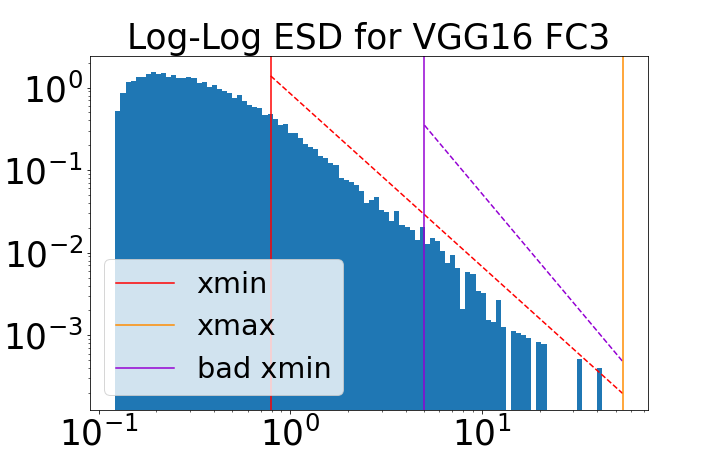
\includegraphics[width=7cm]{./img/fig1-1a.png}
      \label{fig:log-log-esd}
    }
    \subfigure[Lin-Lin ESD]{
      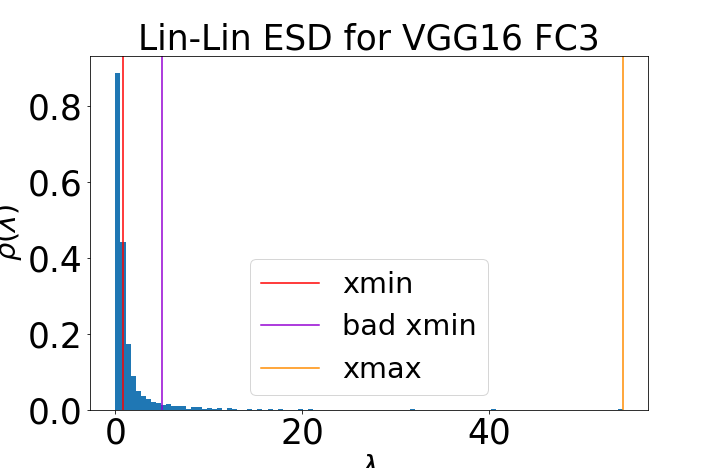
\includegraphics[width=7cm]{./img/fig1-1b.png}
      \label{fig:lin-lin-esd}
    }
    \subfigure[Log-Lin ESD]{
      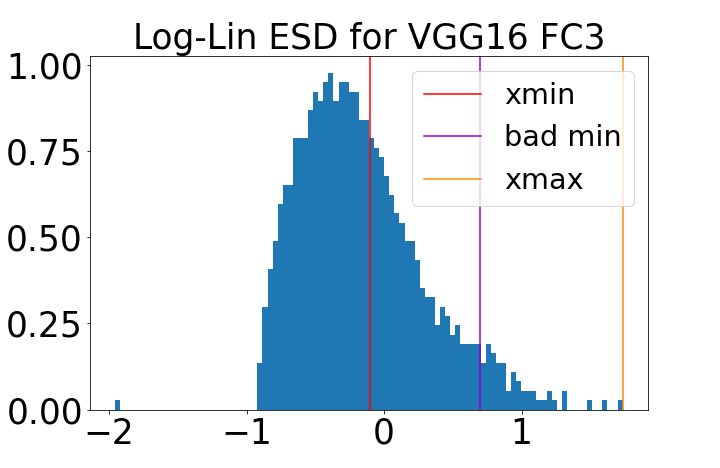
\includegraphics[width=7cm]{./img/fig1-1c.png}
      \label{fig:log-lin-esd}
    }
    \subfigure[$\LambdaMin$ vs KS distance]{
      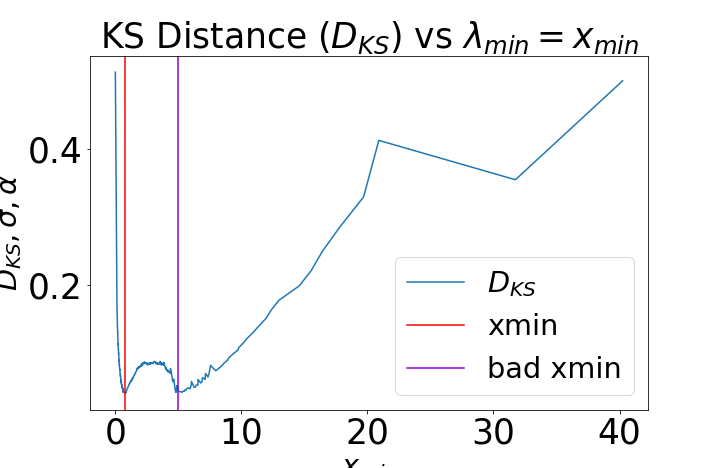
\includegraphics[width=7cm]{./img/fig1-1d.png}
      \label{fig:xmin-DKS-esd}
    }                                     
    \caption{\textbf{Fitting ESDs within \HTSR.} 
         Depiction of the ESD and results of PL fits for a typical well-trained layer of a modern NN (FC3 of VGG19), including both the actual and good PL fit (red) and a hypothetical bad PL fit (purple). 
         The same ESD is plotted on a Log-Log (a), Lin-Lin (b) and Log-Lin (c) scales.
         (d) depicts how the start of the PL tail, $\LambdaMin$, varies with the quality of the PL fit (the $D_{KS}$ distance). 
         All plots are generated using the open-source \WW tool. 
         See the main text for details.
    }
  \label{fig:log-esds}
\end{figure}   


%% %Figure~\ref{fig:log-esds} (from Figure~1 of~\cite{MM21a_simpsons_TR}) displays layer ESD plots for a \Typical layer $\mathbf{W}$,
%% %on different scales (\ref{fig:log-log-esd}, \ref{fig:lin-lin-esd}, \ref{fig:log-lin-esd}),
%% %along with the quality of fit ($D_{KS}$ vs. $x_min$, \ref{fig:xmin-DKS-esd}), as generated with the~\WW~tool,
%% %\footnote{The \WW~tool finds the best PL fit automatically and reproducibly.}

\paragraph{Fitting ESDs.}
Choosing the start of the tail, $\LambdaMin$, is important for \HTSR (and it will be very important for \SETOL, as we will describe below).
See Figure~\ref{fig:log-esds} for a depiction of how this was done within \HTSR theory.
Figures~\ref{fig:log-log-esd}-\ref{fig:log-lin-esd} show the results of both a ``good fit'' and a ``bad fit'' on the same ESD,
while Figure~\ref{fig:xmin-DKS-esd} indicates the quality of fit.
For the good fit, the start of the tail is the optimal value $\LambdaMin=xmin$ (in red); and for the bad fit, it is a suboptimal $bad\;xmin$ (purple).
Figure~\ref{fig:xmin-DKS-esd} depicts how the best fit is determined; it plots $xmin=\LambdaMin$ versus the $D_{KS}$ 
value, which is the Kolmogorov-Smirnov (KS) distance between the PL fit and the empirical data~\cite{CSN09_powerlaw}.
Notice that there are two nearly degenerate minima on Figure~\ref{fig:xmin-DKS-esd}, corresponding to the good fit and the bad fit. 
It is not uncommon to face such practical challenges, as real-world ESDs are often slightly deformed from a perfect PL density, e.g.,
they may have two or more near-degenerate solutions on the KS plots (d).
(They may also have anomalously large eigenvalues; this is discussed in more detail in Section~\ref{sxn:HT_ESDs}.)

When one finds a good PL fit for the ESD of a layer $\mathbf{W}$,
it provides information about the \SHAPE~and \SCALE~of the ESD of that layer.
In particular: 
the \SPECTRALNORM, $\lambda_{max}$, being a matrix norm, is a measure of the size \SCALE~of the ESD~\cite{MM21a_simpsons_TR}; 
the fitted PL exponent \ALPHA, $\alpha$, being the slope of the tail of the ESD on a Log-Log plot, describes the \SHAPE~of the ESD; and
the \WW \ALPHAHAT~metric combines \SHAPE~and \SCALE~information.
Also, as opposed to other applications of PL fits~\cite{CSN09_powerlaw,BouchaudPotters03}, in our analysis,
the start of the tail, $\LambdaMin=\LambdaPLmin$, plays a particularly important role because it
identifies the subspace of the strongest generalizing eigencomponents (i.e., $\XECS$, below) in each layer.

\begin{table}[t] %[ht!]
\begin{center}
  \begin{tabular}{| l | c | c | r | }
    \hline
    HT/\RMT Universality class & $\mu$ range   & $\alpha$ range    & Best Fit  \\ \hline \hline
    RandomLike            & NA            & NA                & MP        \\ \hline
    Bulk+Spikes           & NA            & NA                & MP+Spikes \\ \hline
    Weakly Heavy Tailed   & $\mu > 4$     & $\alpha>6$        & PL        \\ \hline
    Heavy (Fat) Tailed    & $\mu\in(2,4)$ & $\alpha\in(2,6)$  & PL        \\ \hline
    Very Heavy Tailed     & $\mu\in(0,2)$ & $\alpha\in(1,2) $ & (T)PL     \\ \hline
    Rank Collapse       & NA            & NA                & NA        \\ \hline
  \end{tabular}
\end{center}
\caption{\HTSR~Heavy-Tailed Universality classes of \RMT. See Table~1 of \cite{MM18_TR_JMLRversion} for more details.    }
\label{tab:Uclass}
\end{table}



\subsection{Gaussian and Heavy-Tailed Universality}
\label{sxn:guass_ht_univ}

The \HTSR \Phenomenology uses \RMT to classify of the ESD of a layer $\mathbf{W}$ into one of 5+1 Phases of Training, 
each roughly corresponding to a (Gaussian or HT) Universality class (of \RMT or \HTRMT).
This is summarized in Table~\ref{tab:Uclass}. 
A Universality class is a set of matrices having a common limiting spectral distribution, regardless of the other properties of their entries. 
Of those, the most familiar is the Gaussian class, characterized by the Marchenko Pastur (MP) results from traditional \RMT~\cite{EW13,potters_bouchaud_2020}. 
The Gaussian Universality class, however, is particularly poorly suited for analyzing realistic NNs---precisely
because the ESDs of SOTA NNs are well-fit by HT distributions.
This should not be surprising: weight matrices of realistic NNs do \emph{not} have independent (i.i.d.)
entries---their entries are strongly-correlated precisely because they provide a view into the correlated training data.

To model strongly-correlated NN layer matrices, the \HTSR \Phenomenology characterizes NN layer weight matrices
in terms of their ESDs (when a good PL fit can be found) by postulating that the (tail of the) eigenvalue spectrum $\rho(\lambda)$ 
determines how each layer contributes to the overall generalization.  
To do this, the \HTSR approach models the strong-correlated layer weight matrices \emph{as if} they are actually i.i.d. HT random
(i.e., entry-wise uncorrelated) matrices. 
By doing this, one can  associate each $\rho(\lambda)$ with 
the corresponding HT Universality class, according to the PL exponent $\alpha$ fitted from the ESD. 
As we will see in 
Section~\ref{sxn:HT_ESDs}, it can be critical to distinguish  when the ESD is HT\emph{Correlation-wise} vs HT \emph{Element-wise}.
\michael{MM TO DO: refine that sentence, in light of similar such changes I'll make above.}

To understand Table~\ref{tab:Uclass} better, we first review basic results.  %% from (Gaussian and HT) \RMT.


\subsubsection{\RandomMatrixTheory (\RMT):  Marchenko-Pastur (MP) Theory and Tracy-Widom (TW) Fluctuations}

\begin{figure}[t] %[h]
    \centering  
    \subfigure[MP, varying $Q=\tfrac{N}{M}$]{ 
      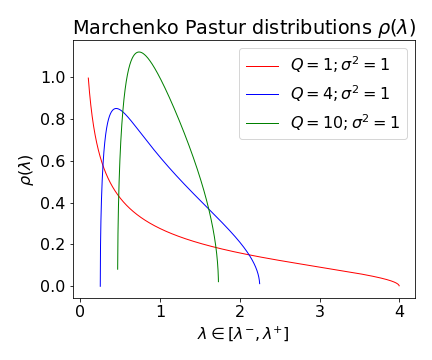
\includegraphics[width=7.0cm]{./img/mp-Q.png}
      \label{fig:MP-esds-a}
    }                               
    \subfigure[Tracy Widom fluctuations]{
      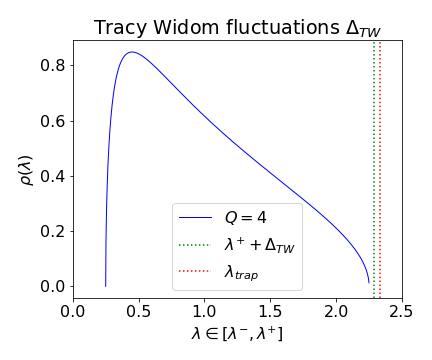
\includegraphics[width=7.0cm]{./img/mp-TW.png}
      \label{fig:MP-esds-b}
    }                    
    \caption{MP distributions for different aspect ratios $Q$ and variance scales $\sigma^2$, and an example of the finite-sized TW fluctuation $\Delta_{TW}$. }
   \label{fig:MP-esds}
\end{figure}

The Marchenko-Pastur (MP) distribution predicts the (limiting) \SHAPE of an ESD, $\rho_{MP}(\lambda)$, when the layer weight matrix has elements that are i.i.d. random from the Gaussian \Universality class.
%%As such, \HTSR theory is particularly useful when the ESD deviates from the MP predictions.
In particular, the ESD will be MP when the matrix elements are drawn from a Normal distribution $W_{i,j}\in  N(0,\sigma^{2})$, e.g., as is typical at initialization, before NN training begins.
Figure~\ref{fig:MP-esds} (from Figure~4 of \cite{MM18_TR_JMLRversion}) displays the MP distribution for different aspect ratios $Q=\tfrac{N}{M}$ and variances $\sigma^{2}$.  
Notice that the \SHAPE is characterized by a well-defined, compact envelope with sharp edges.

The MP distribution also predicts the \SCALE of an ESD, again when the layer weight matrix has elements that are i.i.d. random from the Gaussian \Universality class.
In particular, an MP distribution, $\rho_{MP}(\lambda)$, has very crisp, well-defined lower and upper bounds $\lambda^{-},\lambda^{+}$~\cite{MM18_TR_JMLRversion}, and (importantly) the upper bound $\lambda^{+}$ exhibits finite-size Tracy-Widom (TW) fluctuations, $\Delta_{TW}(\lambda)$, which are on the order of $\mathcal{O}(M^{-2/3})$. 
Thus, any layer eigenvalue with \SCALE greater than this, i.e., $\lambda>[\lambda^{+}+\Delta_{TW}(\lambda)]$, is an ``outlier'' or a ``spike.''

According to the \HTSR \Phenomenology, these spikes carry significant generalizing information. 
(This is well-known for Bulk-Plus-Spike models~\cite{MM18_TR_JMLRversion}, but the \HTSR \Phenomenology generalizes this concept.)
%
Relatedly, for layer matrices $\mathbf{W}$ with aspect ratio $Q>1$ (i.e., rectangular matrices, where $N>M$), MP \RMT predicts there should be no zero eigenvalues, i.e., $\lambda_i>0$, for all $i$. 
Generally speaking, for well trained NNs, for layers with $Q>1$, all eigenvalues are strictly larger than zero, i.e., 
well-trained layer weight matrices, with $Q>1$, should have full rank and exhibit no ``rank collapse.'' 
\michael{MM TO DO: that sentence needs to go elsewhere.}
\HTSR places random Gaussian and ``Bulk-Plus-Spike'' matrices into the first two rows of Table~\ref{tab:Uclass}.
The essential feature of Gaussian random matrices is that their entries have no correlations. 
When some correlations are injected, a few large spike eigenvalues form, without otherwise disturbing the shape of the ESD. 
\michael{MM TO DO: put in comment about how bulk-plus-spike is just a perturbative variant of MP.}
To really understand how individual NN layers converge, we need to understand when and why their ESDs become HT.


\subsubsection{\HeavyTailed \RandomMatrixTheory (\HTRMT) and \PowerLaw (PL) fits}
\label{sxn:htsr_pl_fits}

For very well-trained NN layers, ESDs are \emph{not} MP at all.
Frequently, if not always, their ESDs are HT---and they are HT \emph{because} they are strongly-correlated matrices.  
Importantly, they are \emph{not} HT element-wise.
Instead, their entries have a scale, and they have ESDs that are HT due to correlations learned during training. 
Existing theoretical approaches, including \SLT and even \STATMECH, cannot readily model such strongly-correlated systems.%
\footnote{For example, such theoretical approaches typically deal better with \emph{\Scale} information (such as $\lambda_{max}$) than with 
\emph{\Shape} information (such as $\alpha$), e.g., by characterizing an ``eigen-gap'' separating large eigenvalues from 
``noise''~\cite{bach2006_JMLR} according to a noise plus low-rank perturbation model~\cite{BFR11}.}

Such strongly-correlated systems, however, do frequently arise in other, related scientific domains, including
in the \STATMECH of self-organizing systems~\cite{bak97a,SornetteBook}, 
in electronic structure theory~\cite{Martin1996,Martin1998,Martin1996_CPL}, and
in quantitative finance~\cite{bouchaud1999,bouchaud2005,potters_bouchaud_2020}. 
In these (and other) domains, correlated systems frequently exhibit characteristic PL signatures; and it is common practice to \emph{model} correlated systems as random (uncorrelated) systems by using HT statistics (e.g., Levy distributions or PL random matrices), fully understanding that such systems are by no means actually i.i.d. random.
The \HTSR \Phenomenology builds upon this longstanding practice by 
%providing a qualitative \Phenomenology that characterizes the layers in well-trained NNs.
delimiting families of HT NN weight matrices based on the corresponding Universality classes of Pareto matrices. 

We explain briefly how to interpret Table~\ref{tab:Uclass} with respect to \HTRMT. The 5+1 Phases of Training can be 
identified by fitting ESDs to MP or PL distributions, whichever gives the best fit, as shown in the last column.
In case the PL distribution is a better fit, \HTSR \Phenomenology treats the layer weight matrix as 
equivalent to an i.i.d. random matrix $\mathbf{W}(\mu)$, whose elements have been drawn from a Pareto distribution 
with exponent $\mu$. 

\paragraph{Heavy-Tailed Universality Classes of Random Pareto Matrices}
For such an element-wise HT matrix, the theoretical \emph{limiting} ESD of a Pareto matrix is also PL,
which allows us to related the fitted PL $\alpha$ with exponent $\alpha=a\mu+b$, to the Pareto exponent $\mu$.
Ideally, for an infinite width matrix ,  $a=\tfrac{1}{2}$ and $b=1$, but due to finite-size effects, however,
we have found we must take $a\ge \tfrac{1}{2}$ and $b\ge 1$, giving
\begin{align}
W_{i,j}(\mu)\sim\dfrac{C}{x^{\mu +1}},\;\;\;\rho(\lambda)\sim\lambda^{-(a\mu+b)}.
\end{align}
According to the above relation, 
we can use either the fitted PL exponent $\alpha$, or the Pareto exponent $\mu$,
to index the HT Universality classes,
Note, however, that the finite-size effects strongly depend on  the and aspect ratio  $Q=N/M$,
at least when applied to i.i.d random Pareto matrices, and 
the (Clauset MLE) PL fit may overestimate the $\alpha$ of the ESD.
Table~\ref{tab:Uclass} delimits the HT matrices 
into sub-categories (as shown in the bottom four rows)  based on the behaviors of $\alpha$ as a function of $\mu$.

Figure~\ref{fig:HT-esds} illustrates how the fitted PL exponent $\alpha$ corresponds to the actual Pareto exponent $\mu$ 
for different aspect ratios $Q=M/M$.
Figure~\ref{fig:HT-esds-a} displays the ESDs of three different i.i.d. $1000\times1000$ HT random matrices, with $\mu=1,3,5$, on a Log-Log scale.  
Notice that smaller $\mu$, and therefore smaller $\alpha$, corresponds to heavier (i.e., larger) tails.
Figure~\ref{fig:HT-esds-b} shows how the empirically fit PL exponent $\alpha$ can vary with the theoretical $\mu$ for an associated $\mathbf{W}(\mu)$.
For $\mu<2$ and $Q=1$, the fitted $\alpha$ follows the linear relation $\alpha=\frac{1}{2}\mu+1$,
albeit with some error.
In contrast, for the more relevant $\mu \in (2,4)$ regime, the relation now depends far more 
strongly on the aspect ratio $Q$, and $\alpha\in[2,6]$.
For $\mu>4$, the fitted $\alpha$ saturates for each specific value of $Q$.

We emphasize that we only model the ESDs of the NN layer weight matrices using the
same Universality class to that associated with the ESD of a random, i.i.d, HT Pareto matrix.
In fact, the elements $W_{i,j}$ do not at all appear as if they have been
drawn from an HT Pareto distribution, and, in contrast, are almost always well fit to a Laplacian distribution.
Also, despite these strong finite-size effects, empirically one finds that the ESDs arising large, well trained,
modern NNs can frequently be well fit to a PL (or TPL), and that the fitted $\alpha\in [2,6]$ for $80-90\%$
of NN layers.  Notably, we rarely find $\alpha<2$ in the best performing, open source, pretrained DNNs.

\charles{Not sure where to put this..see text also}
%Despite the fact that Correlation-wise HT matrices found in NNs and Element-wise HT Pareto matrices arrive at their
As there is \emph{no} ground truth whatsoever as to the limiting spectral density of a strongly-correlated NN weight matrix
(especially without HT elements)
the \HTSR \Phenomenology uses Pareto matrices as a guide. 
However, as we will see in Section~\ref{sxn:HT_ESDs}, this analogy should be treated with caution because there are 
cases where it breaks down.

No matter why a matrix ESD is HT, it can be difficult to reliably estimate the $\alpha$ parameter when
the true $\alpha$ is large. For Pareto matrices of the size investigated here, 
an observed $\alpha$ above $6$ is uninformative --- the tail will decay very rapidly indeed,
leaving very little of it to study.
In this sense, the HT Universality classes are \emph{larger} than the set of only strongly-correlated 
matrices or Pareto random matrices.



%and they can be used to model the strongly-correlated weight matrices $\mathbf{W}$---as long as we are careful to distinguish 
%between when $\mathbf{W}$ is element-wise HT and when $\mathbf{X}$ is correlation-wise HT. 
%HT because $\mathbf{W}$ is strongly-correlated.

\begin{figure}[h]
    \centering  
    \subfigure[Heavy Tailed ESDs]{ 
      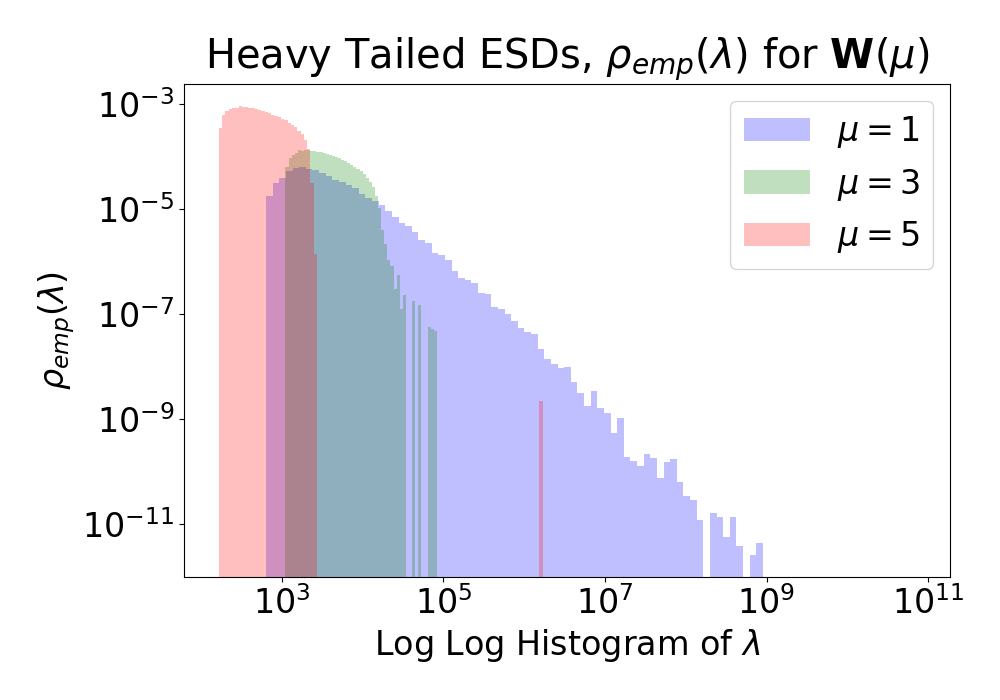
\includegraphics[width=7cm]{./img//heavy-tailed-log-log-esds.png}
      \label{fig:HT-esds-a}
    }                               
    \subfigure[PL $\alpha$ vs HT $\mu$ exponent]{
      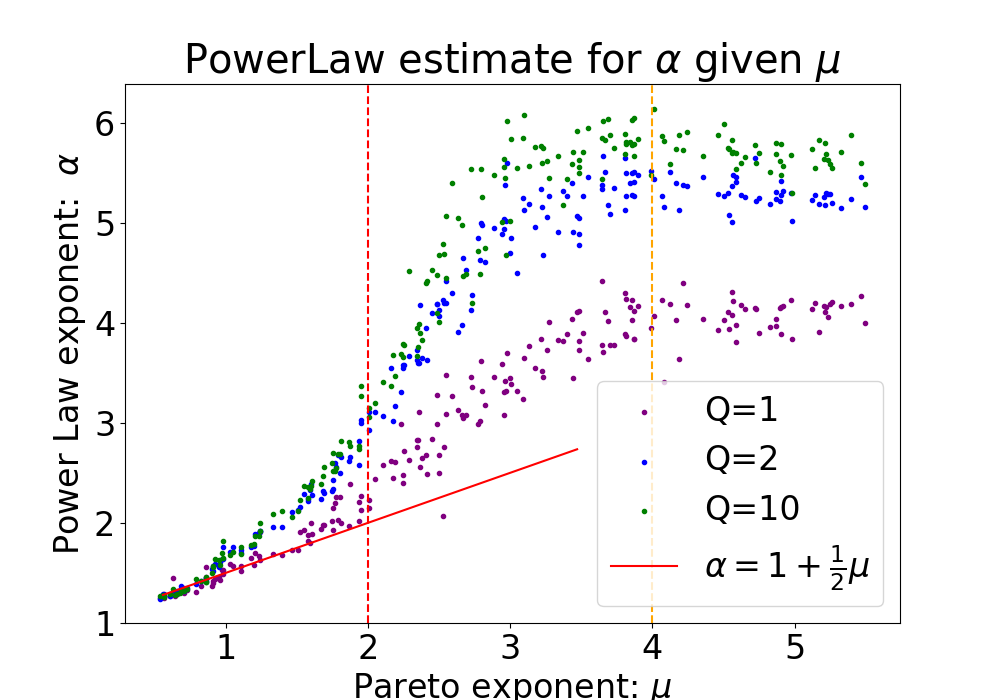
\includegraphics[width=7cm]{./img/alpha-mu-plot2.png}
      \label{fig:HT-esds-b}
    }                                                                                                                            
    \caption{Comparison of ESDs and Power Law (PL) exponents $\alpha$ from Heavy-Tailed (Pareto) 
weight matrices $\mathbf{W}(\mu)$. 
Subfigure (a) depicts 3 \Typical ESDs with Pareto exponent $\mu=1,3,5$, each decreasing in \SHAPE~and \SCALE.
Subfigure (b) shows how the exponent $\alpha$ of the PL fit varies with $\mu$, with significant finite-size
effects emerging for $\mu>2$ and $\alpha>2$.
}
   \label{fig:HT-esds}
\end{figure}

There is a particularly important boundary between Universality classes where $\alpha = 2$. Recall that one of the 
properties of power law distributions $\rho(\lambda)\sim \lambda^{-\alpha}$ is that if $\alpha<2$, than the variance of 
$\rho(\lambda)$ is infinite. In such cases, the variance cannot be estimated empirically, making $\rho(\lambda)$ in 
some sense \emph{\ATypical}. This implies that the NN will have substantially greater difficulty in applying any further 
load to such a weight matrix. Thus, the value of $\alpha = 2$ is a \emph{critical value}. (See 
Figure~\ref{fig:mlp3-FC1-alpha-overloaded} in Section~\ref{sxn:hysteresis_effect} for an empirical study of this effect 
in a small MLP.)

%When fitting ESDs of well-trained models, 
Smaller PL exponent $\alpha$ values correspond to heavier tails, $\rho_{tail}(\lambda)$; and
the \HTSR \Phenomenology observes that smaller PL exponents $\alpha$ (at least for $\alpha\in(2,6)$) tend to correspond to better models.
This is the key idea of the \HTSR:
the generalizing components of a layer matrix $\mathbf{W}$ concentrate in larger singular vectors associated with the tail, and 
so that better models have more slowly-decaying (i.e., larger) ESD tails.
This differs significantly than simply taking a general low-rank approximation to $\mathbf{W}$, where the rank
is chosen without insight from the \HTSR \Phenomenology. 
The \SETOL theory formalizes this observation as a key assumption. We will revisit these model selection questions in 
Section~\ref{sxn:setol_overview} below.




\subsection{Data-Free \SHAPE and \SCALE \Quality Metrics}
\label{sxn:htsr-metics}

The \HTSR \Phenomenology provides quality metrics for both individual layers and (by averaging layers) for an entire NN model.

\paragraph{Layer-wise Quality Metrics.}
Using the \HTSR \Phenomenology, we can define several other \SHAPE and/or \SCALE based layer (quality) metrics.
These are available in the \WW tool, and they work very well in practice.
\begin{itemize}
\item 
\ALPHA 
$(\alpha)$: $\rho_{tail}(\lambda)\sim\lambda^{-\alpha}$. 
A \SHAPE-based quality metric.
\item
\LOGSPECTRALNORM: $\log_{10}\lambda_{max}$.
A \SCALE-based quality metric.
\item 
\ALPHAHAT 
$(\hat{\alpha})$: $\alpha\log_{10}\lambda_{max}$.
A \SCALE-adjusted \SHAPE-based quality metric.
\item
\RANDDIST: $JSD[\rho^{emp}|(\rho_{rand}^{emp})]$.
A \SHAPE-based, non-parametric quality metric, suitable for highly-accurate, epoch-by-epoch analysis.%
\footnote{JSD is the Jensen-Shannon Divergence between the original ESD and the ESD of the layer weight matrix, randomized element-wise.}
\item
\PLKS: $D_{KS}$.
The KS-distance, or quality-of-fit, of the PL fits.  
For transformers, foundation models, and large, complex, modern NNs, this is frequently an even better model quality metric than the $\alpha$ of the PL fit itself.
\item
\MPSOFTRANK: $\mathcal{R}_{MP}$.
The MP-SoftRank, defined in~\cite{MM18_TR_JMLRversion}, can be used to identify problems such as when there is significant label or data noise that causes spuriously small $\alpha$, and also when it is difficult to fit a PL law.%
\footnote{The~\WW tool also implements the WW-SoftRank, which is like the MP-SoftRank, but replaces $\lambda_{bulk}^{+}$ with $\lambda_{rand}^{max}$; these are mostly equivalent for large matrices, but they can be different for very small matrices.}
\end{itemize}

\noindent
Each of these quality metrics provides a simple characterization of the \SHAPE and/or \SCALE of the tail of the ESD of a given layer $\mathbf{W}$.
These metrics are related to each other, and they have various trade-offs in practice~\cite{MM20a_trends_NatComm, MM21a_simpsons_TR, YTHx23_KDD}.
Of particular interest here in our development of \SETOL are the PL-based \WW~\ALPHA and  \ALPHAHAT~metrics.


\paragraph{From Layer-wise Quality Metrics to Layer-Averaged Model Quality Metrics.}
One can use the \HTSR \Phenomenology to go beyond individual \LayerQuality metrics, to construct model quality metrics by averaging \LayerQuality metrics (over all layers that are not very small). 
%%The PL \ALPHA and  \ALPHAHAT metrics in particular correlate remarkably well with reported test accuracies for a wide range of large and very well trained NN models~\cite{MM20a_trends_NatComm,MM19a_TR}.
Existing \HTSR model quality metrics implicitly require that all layers are statistically independent, so that the average model quality is just the average of the contributions from each weight matrix $\mathbf{W}$.%
\footnote{This independence assumption, clearly a mathematical convenience, gets us closer to a workable theory. One could go beyond a ``single layer theory'' by adding in intra-layer correlations empirically. The \WW tool does support this, but doing so is outside the scope of this work.}
%
Given a \LayerQuality metric, $\Q^{NN}_{L}(\mathbf{W})$, one can define the \emph{\ModelQuality} $\Q^{NN}$ metric for an entire model as 
\begin{align}
\label{eqn:ProductNorm}
\Q^{NN}&:=\underset{L}{\prod}\;\Q^{NN}_{L}(\mathbf{W}) ,
\end{align}
a product of each independent \LayerQuality $\Q^{NN}_{L}$, and then consider the layer average as the log \emph{\LayerQuality},
\begin{align}
\label{eqn:LogProductNorm}
\log\Q^{NN}=\frac{1}{N_{L}}\underset{L}{\sum}\;\log\Q^{NN}_{L}=\langle\log\Q^{NN}_{L}\rangle_{\bar{L}}
\end{align}
where $\langle\;\cdots\;\rangle_{\bar{L}}$ denotes the layer average.

In particular, prior work has used the following metrics:
\begin{itemize}
\item
The layer-averaged model quality metric \ALPHA, $\log\Q^{NN}=\langle\alpha\rangle_{\bar{L}}$, describes the \SHAPE of the ESDs.
One can use the averaged \ALPHA when studying a single model, and only varying the regularization hyperparameters, although \ALPHA also works very well as a model quality metric when comparing different transformer models~\cite{YHTx21_TR}.
\item
The layer-averaged model quality metric \LOGSPECTRALNORM, $\log\Q^{NN}=\langle\log\lambda_{max}\rangle_{\bar{L}}$, describes the \SCALE of the ESDs.
The averaged \LOGSPECTRALNORM does work as a model quality metric but not as well as \ALPHA~(or \ALPHAHAT).
Notably, \SLT predicts that smaller, not larger, \LOGSPECTRALNORM should be correlated with model quality; the opposite is observed in practice!
This is because smaller layer $\alpha$ generally, but not always, corresponds to larger $\lambda_{max}$.%
\footnote{The \LOGSPECTRALNORM can exhibit a Simpson's paradox when segmenting models by quality)~\cite{MM21a_simpsons_TR}.  Nevertheless, this metric may be useful when a PL fit can not be obtained, say, when $N\gg M$ and $M$ is very small, as with LSTMs,  U-Net architectures, etc.}
\item
The layer-averaged model quality metric \ALPHAHAT, $\log\Q^{NN}=\langle\alpha\log\lambda_{max}\rangle_{\bar{L}}=\langle\hat{\alpha}\rangle_{\bar{L}}$, incorporates both \SHAPE and \SCALE information.
This can compensate for anomalies that can arise when (say) comparing models of different sizes or model qualities~\cite{MM21a_simpsons_TR} or when other issues cause unusually large $\lambda_{max}$. See Section~\ref{sxn:Traps}).
\end{itemize}

\noindent
The layer-averaged \ALPHAHAT model quality metric has been applied in a large meta-analysis of hundreds of SOTA 
pre-trained publicly-available NN models in CV and NLP~\cite{MM20a_trends_NatComm,YTHx22_TR,YTHx23_KDD,MM19a_TR}. 
%
Generally speaking, \HTSR shape-based metrics, when used appropriately, outperform all other metrics studied (including 
those from \SLT, and with access to the training/testing data,) for predicting the quality of SOTA pre-trained publicly-available NN models.  
%
The \HTSR theory predicts that the best-performing NN models have layers with $\ALPHA\in[2,6]$, and with $\alpha=2$
indicating optimal performance.
Moreover, prior empirical results show that the \ALPHA and \ALPHAHAT~metrics can predict trends in the \Quality 
(i.e., the \GeneralizationAccuracy), of SOTA NN models---\emph{even without access to any training or testing data}~\cite{MM20a_trends_NatComm}.
\michaeladdressed{Somewhere, around here, we need to be more explicit that we want $\alpha$ in $[2,4]$, with lower better, and that for \HTSR the latter comes from more of an informal argument from other areas that we squeeze more juice from the data; but it is not derived, even semi-empirically, from an underlying theory.}





\newpage
\section{A \SemiEmpirical Theory of (Deep) Learning (\SETOL)}
\label{sxn:setol}
Based on prior empirical results, and the success of the \ALPHA and \ALPHAHAT metrics that are based on the \HTSR \Phenomenology, this leads to the deeper question: 
%
\begin{quote}
\emph{Why do the \ALPHA and \ALPHAHAT metrics work so well as NN model quality metrics for SOTA NN~models?}
\end{quote}
That is, why do NN models with heavier-tailed layer Empirical Spectral Distributions  (ESDs) tend to generalize better when compared to related models, and how can single-layer metrics predict model quality so well ?
Relatedly, can we derive these metrics from first principles?
(If so, then under what conditions do they hold, and under what conditions do they fail?)

\noindent
To answer these questions, we will derive a general expression for the \LayerQuality, $\Q$, of an NN.
Although many modern NNs have many layers, we adopt a single-layer viewpoint (like a matrix-generalized Student–Teacher) because in \StatisticalMechanicsOfGeneralization (\SMOG) theory~\cite{SST92,STS90} the multi-layer generalization can be factorized or approximated.
For this, we will obtain by simple averaging our model quality metrics, under effectively a single layer approximation, that correspond to \ALPHA and \ALPHAHAT.


In deriving these quantities, we will introduce to NN theory a new \SemiEmpirical approach that combines techniques from \STATMECH and \RMT in a novel way.must depend on the spectral density
The \LayerQuality $\Q$ will estimate the contribution that an individual NN layer makes to the overall quality of a trained NN model.
In deriving $\Q$, we have discovered a new \LayerQuality metric, called the \TRACELOG condition,
which indicates that the generalizing components of the layer must concentrate into a low-rank subspace which we term the \emph{\EffectiveCorrelationSpace}, or~\ECS. That is, the better this condition is met, the more the generalizing components concentrate in this \ECS, and this tendency provides a new layer quality metric, derived in a totally independent way from \ALPHA and \ALPHAHAT. We will provide strong empirical justification that both metrics are acceptable Quality metrics by showing that they converge as model quality increases.

%\red{[There are forward pointers to \ref{sxn:empirical}, but not to \ref{sxn:matgen}. \ref{sxn:matgen} fulfills the claims of derivation. I suggest to start a new paragraph here, and add one above that does a similar job relating results in Section \ref{sxn:matgen} to claims being made here. This is one of the most critical pages in the whole paper.]}\\
Importantly, we have conducted detailed experiments to show 
that the empirical estimates of the \SETOL \TRACELOG condition align remarkably well with predictions from the \HTSR
theory under \Ideal conditions (see Sections~\ref{sxn:empirical-test_acc}) and, then, 
that the key assumptions of our \SETOL theory are valid
(see Sections~\ref{sxn:empirical-effective_corr_space} and \ref{sxn:empirical-trace_log}).
In Section~\ref{sxn:empirical_comp_r_transforms}, we demonstrate how to apply theory directly using explicit calculations of the \RMT layer cumulants.
We next examine how the \HTSR predictions (i.e., the HT PL exponent $\alpha$) behave under non-\Ideal conditions (see Sections~\ref{sxn:empirical-correlation_trap} and \ref{sxn:hysteresis_effect}).
%
In the following, we will outline key conceptual aspects of \SETOL.
In Section~\ref{sxn:setol_overview}, we give an overview of \SETOL;
In Section~\ref{sxn:ideal_learning}, we describe the conditions of \Ideal learning under \SETOL and how they differ from those of \HTSR; and
In Section~\ref{sxn:HT_ESDs} we describe conditions that deviate from this.

\begin{figure}[htbp]                 % place here / top / bottom / page
  \centering
  % --- scale the entire picture to 75 % ---
  \scalebox{0.75}{% ---------- flowchart.tex ----------
\usetikzlibrary{arrows.meta, positioning, calc}

\tikzset{
  box/.style={
    draw, rectangle, rounded corners=3pt,
    minimum width=4.3cm, minimum height=1.3cm,
    align=center, font=\small
  },
  arrow/.style={-Stealth, very thick},
}

\begin{tikzpicture}[
  node distance = 2.5cm and 2.3cm,
  >=Stealth
]

% ========== ROW 1 ==========
\node[box] (smog)    {\underline{Classic SMOG}\\Student-Teacher Perceptron\\
but with  \\
\textbf{Fixed Teacher (input)}};
\node[box, right=of smog] (overlap)
      { \underline{ST Accuracy (Quality) $\Q^{ST}$} \\
    Thermal Average (AA, high-T) \\
        Overlap $R=\SVEC^{\top}\TVEC$ \\
      $\Q^{ST}=\THRMAVG{R}$ 
      };
\node[box, right=of overlap] (hciz)
      {\underline{Matrix Generalized Quality $\QT$}\\
      HCIZ Integral \\
$\OVERLAP:=\tfrac{1}{N}\SMAT^{\top}\TMAT$ \\
$\QT :=   \THRMAVGIZ{\Trace{\OVERLAP^{\top}\OVERLAP}}$  \
      };

% ========== ROW 2 ==========
\node[box, below=of smog] (rg)
      {
        \underline{Wilson Exact RG Condition (\ERG)}\\
      {Effective Correlation Space (\ECS)}\\[4pt]
      $\AMATN=\tfrac{1}{N}\SMAT\SMAT^{T}$, $\AECS=\mathbf{\hat{P}}^{ECS}\AMATN$ \\[4pt]
      $d\mu(\SMAT)\rightarrow  d\mu(\AMAT) \rightarrow d\mu(\AECS)$ \\[4pt]
      $\sum \ln \LambdaECS = 0 $  , $\LambdaECS \ge \LambdaECSmin $
      };

\node[box, below=of overlap] (tanaka)
      {\underline{Tanaka Result for HCIZ}\\
      \LargeN in $N$ limit \\[6pt]
      $\IZG = \tfrac{1}{N}\ln \int d\mu(\AECS)
      exp[n\beta N \Trace{\tfrac{1}{N}\TMAT^{\top}\AMATN\TMAT}]$\\[4pt] 
      $\QT := \tfrac{\partial }{\partial n}\tfrac{1}{\beta}\IZGINF$
      };

\node[box, below=of hciz] (cumul)
  {\underline{Integrated \RTransforms} \\[4pt]    
     $\QT = \sum_{\LambdaECS}\int_{\LambdaECS_{min}}^{\LambdaECS}R_{\AECS}(z)$ \\[4pt]  
     Student ESD $\AMAT$ $\sim$ Teacher ESD $\XMAT$ \\
   $R_{\AECS}(z) = R_{\XECS}(z)$
   };

% ========== ROW 3 ==========
\node[box, below=of rg] (rforms)
      {\underline{\RTransform choices}\\
      Bulk+Spikes (BS) \\
      Free Cauchy (FC)  \\ 
      Inverse MP (IMP) \\
      L\'evy Wigner (LW) \\
      $\cdots$
};

\node[box, right=of rforms] (alpha)
      {\underline{Derive \HTSR metrics}\\
      Extend \SETOL to non-Ideal cases \\\
      $\alpha$ and $\hat{\alpha}$};

\node[box, right=of alpha] (expv)
      {Experimental\\verification};

% ---------- horizontal arrows ----------
\draw[arrow] (smog)   -- (overlap);
\draw[arrow] (overlap) -- (hciz);

\draw[arrow] (rg)     -- (tanaka);
\draw[arrow] (tanaka) -- (cumul);

\draw[arrow] (rforms) -- (alpha);
\draw[arrow] (alpha)  -- (expv);

% ========== bridge 1 : HCIZ → RG  (↓ → ← → ↓) ==========
\coordinate (hcizDrop) at ($(hciz.south)+(0,-0.9)$);          % fall below Row-1
\coordinate (hcizLeft) at ($(hcizDrop -| rg.north)$);         % horizontal to col-1 x
\draw[arrow] (hciz.south) -- (hcizDrop)                       % vertical
             -- (hcizLeft)                                    % horizontal
             -- (rg.north);                                   % vertical down into RG

% ========== bridge 2 : Cumulants → R-forms (↓ → ← → ↓) ===
\coordinate (cumulDrop) at ($(cumul.south)+(0,-0.9)$);
\coordinate (cumulLeft) at ($(cumulDrop -| rforms.north)$);
\draw[arrow] (cumul.south) -- (cumulDrop)
             -- (cumulLeft)
             -- (rforms.north);

\end{tikzpicture}
}   % path to flowchart.tex (no “.tex” needed)

  \caption{Flowchart of the theoretical concepts used to construct SETOL.}
  \label{fig:cetl-flow}
\end{figure}
\subsection{\SETOL Overview}
\label{sxn:setol_overview}

\charles{Some old text here I need to clean up}

Our \SETOL formulates a parametric expression for the \LayerQuality $\Q$ using a matrix-generalization of the classic \StudentTeacher (ST)
model from the \SMOG theory of the 1990s~\cite{SST92,STS90}, evaluated using
recent advances in the evaluation of so-called HCIZ random matrix integrals~\cite{potters_bouchaud_2020,Tanaka2007, Tanaka2008},
such that the final expression for $\Q$ can be written in terms of empirically measured statistical properties of the layer ESD.
We summarize our basic approach here; see Section~\ref{sxn:matgen} for a detailed derivation, and see Section~\ref{sxn:empirical} for a detailed empirical analysis.

Following the \StudentTeacher (ST) model~\cite{SST92}, 
we first formulate the \GeneralizationError $(\AVGE^{ST}_{gen})$ of the linear \Perceptron (in the \emph{\AnnealedApproximation},
and in the \emph{\HighTemperature} limit; see Section ~\ref{sxn:SMOG_main}), and 
we then generalize this to the case of a NN $(\AVGE^{ST}_{gen}\rightarrow\AVGE^{NN}_{gen})$, so that we can analyze the \Quality of each layer.
For the \Perceptron, the \GeneralizationError is an Energy, given as $\AVGE^{ST}_{gen}:=\THRMAVG{1-R}$, where $R$ is the ST vector overlap,
and $\THRMAVG{\cdots}$ is a \emph{\ThermalAverage} (defined in Section~\ref{sxn:mathP}),
a Boltzmann-weighted average.
In this case, the model \Quality, $\Q^{ST}$ is exactly the AA, high-T \AverageGeneralizationAccuracy 
\michaeladdressed{still not sure we are using that term correctly, here and elsewhere}
$\Q^{ST}:=1-\AVGE^{ST}_{gen}=\THRMAVG{R}$.
For an MLP or general NN, each layer Energy is associated with a
\LayerQuality $\Q$, which we identify as the average contribution an
individual layer makes to the overall generalized accuracy,
(i.e $1-\AVGE^{NN}_{gen}$) for a multilayer perceptron (MLP).

For technical reasons (below), we will seek the
\emph{\LayerQuality (Squared)} $\QT$, which is defined as the \ThermalAverage
of the matrix-generalized overlap ($\Trace{\OVERLAP^{2}}$),
\begin{align}
  \label{eqn:QT}
  \QT :=   \THRMAVGIZ{\Trace{\OVERLAP^{2}}}
\end{align}
where $\OVERLAP^{2}$ can be thought of as a \Hamiltonian for the \QualitySquared  $(\HBARE=\OVERLAP^{\top}\OVERLAP)$.

In \EQN~\ref{eqn:QT}, the so-called \emph{\Teacher} ($T$) is the NN model under consideration,
%where $\mathbf{T}$ and $\mathbf{S}$  are the \Teacher and \Student layer weight matrices, resp,
and 
%$\mathbf{R}$ 
$\mathbf{R}:=\frac{1}{N}{\mathbf{S}^{\TR}\mathbf{T}}$
denotes the ST overlap operator 
between the \Teacher layer weight matrix $\TMAT$ and a similar \emph{\Student} ($S$) layer weight matrix $\SMAT$.
The notation $\THRMAVGIZ{\cdots}$ denotes a \ThermalAverage over
all \Student weight matrices $\mathbf{S}$ that resemble the \Teacher weight matrix $\mathbf{T}$.
By ``resemble'', the \SETOL approach assumes that 
%$\mathbf{S}$ lies in the same \HTSR Universality class as the $\mathbf{T}$, and, even more, that 
the ESD of $\mathbf{S}$ has the same \emph{limiting} form as $\mathbf{T}$, placing them in the same \HTSR Universality class.
This is made more precise below.

Let us now express the average matrix-matrix overlap $\mathbf{R}$ in squared form using:
\begin{align}
  \label{eqn:R2}
\Trace{\OVERLAP^{2}} &:=\OLAPSQD  \\ \nonumber
&=\frac{1}{N^{2}}\Trace{\mathbf{T}^{\TR}\mathbf{SS}^{\TR}\mathbf{T}}
=\frac{1}{N}\Trace{\mathbf{T}^{\TR}\mathbf{A}_2\mathbf{T}}
\end{align}
where $\AMAT_{2}$ is the $N\times N$ form of the \Student correlation matrix,
$\mathbf{A}_2:=\frac{1}{N}\mathbf{SS}^{\TR}$.
We will also define the $M\times M$ matrix, $\AMAT_{1}=\frac{1}{N}\mathbf{S}^{\TR}\mathbf{S}$,
used later.

\michaeladdressed{Clarify.}
%It is argued that the \Student and \Teacher weight matrices (i.e., $\TMAT, \SMAT$) have
%specific generalizing eigencomponents that, after training,
%concentrate in a low rank subspace, called the \emph{\EffectiveCorrelationSpace} (\ECS)
%(and that this space satisfies the \TRACELOG condition, described below).
%This is both consistent with the empirical observations and necessary to apply the HCIZ integral
%methods, both described below.
\michaeladdressed{MM TO DO: Dense.  Where is the best place for this par.}

As explained in Section~\ref{sxn:mathP}, this \QualitySquared is more readily obtained as 
the derivative of the \LayerQualitySquared \GeneratingFunction, $\IZG$, defined as
\begin{align}
  \label{eqn:IZG_QT}
  \QT := \dfrac{1}{\beta}\dfrac{\partial }{\partial N} \lim_{N\gg 1}\IZG
\end{align}
$\IZG$ is essentially ($\beta$ times) a \emph{\FreeEnergy} for the (approximate) \LayerQualitySquared.
(see Section~\ref{sxn:SMOG_main}, and the Appendix, Section~\ref{sxn:quality}).
For more details, see Section~\ref{sxn:matgen}, and the Appendix, Section~\ref{sxn:summary_sst92}).

We can write $\IZG$ as an HCIZ Integral, 
\begin{align}
  \label{eqn:QT_dS}
  \IZG  &=  \ln\int d\mu(\mathbf{S})\exp\left(N\beta\Trace{\mathbf{T}^{\TR}\mathbf{A}_2\mathbf{T}}\right),
\end{align}



The \SETOL approach then seeks to express $\IZG$ in~\EQN~\ref{eqn:QT_dS} as an HCIZ integral (and in the large-N limit)~\cite{potters_bouchaud_2020,Tanaka2007,Tanaka2008}.
We evaluate this at large-$N$, and write
\begin{equation}
  \IZGINF:=\lim_{N\gg 1}\IZG
\end{equation}
%%%must restrict the matrices to a lower rank subspace, called the~\ECS,
%%%i.e.,  $\mathbf{\tilde{A}}$. 
%%%We also must change the measure from an integral over \Student weight matrices
%%%to an integral over \Student Correlation matrices, i.e., 
%%%\begin{align}
%%%  \label{eqn:change_measure}
%%%  d\mu(\mathbf{S})\rightarrow d\mu(\mathbf{\tilde{A}}) ,
%%%\end{align}
%%%We can define a single measure for either form of \Student correlation matrix, restricted to the~\ECS,
%%%such that 
%%%$d\mu(\mathbf{\tilde{A}})=d\mu(\mathbf{\tilde{A}}_1)=d\mu(\mathbf{\tilde{A}}_2)$.
%%%This will be important as we need the form $\AMAT_1$ to derive the \TRACELOG condition, below, but
%%%we  formulate the  $\IZG$ using the form $\AMAT_2$.
%%%%Also, and importantly, the change in measure from $d\mu(\mathbf{S})$ to $d\mu(\mathbf{\tilder{A}})$
%is needed in order to apply the HCIZ  integral.
\michaeladdressed{I feel like expositionally it may be good to highlight this in the intro also and to have a bullet highlighting the rule from \HTSR for selecting the generalizing subspace; that will make it easier in the next subsection to highlight how the two connect.}
\charles{Lets discuss.  The intro has some of this. and a lot more}
With these definitions in place, moving forward, the following key assumptions, which can be tested empirically, must hold:
\begin{itemize}
  \item
  \textbf{The Effective Correlation Space (\ECS) Condition.}
  The generalizing components of the \Student (and \Teacher) layer weight matrices concentrate into a lower rank subspace---the~\ECS---spanned by the
  eigenvectors associated with the (heavy) tail of the layer ESD $\rho_{tail}(\lambda)$, such that the test error can 
  be reproduced with only these components. 
  \michael{MM TO DO: we need to define tail better somewhere, but see also my comment above about presenting the two generalizing subspaces better.}
  We write $\AECS$ to denote the projection of the correlation
  matrix $\AECS:=\mathbf{P}_{ecs}\AMAT$, onto this subspace, now with rank $\MECS\ll M$.
  This restricts the measure $d\mu(\AMAT)$ to the~\ECS, $(d\mu(\AMAT)\rightarrow d\mu(\AECS))$.
  This assumption will empirically examined using real-world \Teacher weight matrices $\TMAT=\WMAT$
  in Section~\ref{sxn:empirical-effective_corr_space}. 
%  Importantly, this lets interpret the \EQN~\ref{eqn:QT_HCIZ}  as acting only in this subspace.
  \item
  \textbf{The \TRACELOG Condition.}
  The \Student correlation matrix $\AECS_1$ (when properly normalized)
  satisfies the condition that $\Trace{\ln\AECS_1}=\ln\Det{\AECS_1}=0$,
  so that the change of measure $d\mu(\SMAT) \rightarrow d\mu(\AECS) $ is Volume Preserving.
  This condition is derived explicitly in terms of $\AECS_1$, and therefore will hold for $\AECS_2$
  (and the Teacher Correlation matrix, $\XECS=\frac{1}{N}\TMAT^{\TR}\TMAT$).
  Practically, this implies that the $\MECS$ eigenvalues $\LambdaECS$
  of the tail of the ESD must satisfy $\sum_{i=1}^{\MECS}\ln\LambdaECS_{i}\approx 0$.
  Experiments will test this assumption explicitly in Section~\ref{sxn:empirical-trace_log}.
\end{itemize}
Remarkably, both conditions hold best empirically when the \HTSR PL quality metric $\alpha\gtrsim 2$ is \Ideal. Motivated from these empirical observations, we have:
\begin{itemize}
  \item
  \textbf{$\IZGINF$ is expressed as an HCIZ integral, at large-$N$.}
  We have
  \begin{align}
  \label{eqn:IZGINF_HCIZ}
  \IZGINF = \lim_{N\gg 1}\ln\int d\mu(\AECS)\exp\left(\beta\Trace{\mathbf{T}^{\TR}\AECS_2\mathbf{T}}\right) %= \beta\sum_{i=1}^{\MECS}\GNECS
  \end{align}
  where  measure $d\mu(\AECS)$ lets us average over all \Student Correlation matrices $\AECS_{2}$ which
  lie in the~\ECS space and which ``resemble'' the \Teacher, 
  where by ``resemble'' we mean that they share the same form of the tail of
  their limiting ESDs,
  i.e., $\rho^{\infty}_{\AECS}(\lambda)\sim\rho^{\infty}_{\XECS}(\lambda)$.
  \item
  \textbf{The Layer Quality (Squared) $\QT$ is a~\GEN.}
  \michael{We need to figure out what to call that, I think norm isn't right, is it a generating function.}
  \charles{OK go ahead.}
  The final expression for $\QT$ can be written as the derivative of $\IZGINF$  as
  \begin{align}
    \label{eqn:QT_result}
    \QT = \dfrac{1}{\beta}\dfrac{\partial}{\partial N}\IZGINF = \sum_{i=1}^{\MECS}\GNI
  \end{align}
  where $\GNI$ is a \emph{\GEN}, and is  defined as the integrated \emph{\RTransform} $R(z)$ of the \Teacher
  layer ESD (where $z\in\mathbb{C}$), such that $\GN:= \int_{\LambdaECSmin}^{\lambda}R(z)dz$
  and $\LambdaECSmin$  encapsulates  the~\ECS (and selects the desired branch-cut of $R(z)$
  so that it is both single-valued and analytic).
\end{itemize}


\michael{MM TO DO: Somewhere we need to distinguish between \SemiEmpirical in general and our specific \SETOL approach.}
%\charles{TRY THIS: These two key, testable assumptions allow \SETOL to move beyond the \HTSR \Phenomenology to derive a more rigorous expression of model \GeneralizationError. It does so by leveraging spectral properties of weight matrices that permit deeper characterization of ways in which weight \emph{matrices} can be similar -- or \ATypical -- which is something parameter \emph{vectors} cannot.}
%\michael{No, I understand that.  What I am asking is: how do we want to describe the difference between \SemiEmpirical and \SETOL?  I think \SETOL is our particular model and setup; but \SemiEmpirical is a more general approach (meaning, in particular, it may not need a bolded name here).  }
%\charles{OK, well we have a section (140) where we discuss nuclear physics; what about there ?}

To apply the theory, one must choose an \RTransform $R(z)$ for	the \Teacher that models 
the tail of the ESD $\rho^{emp}_{T}(\lambda)$, and that can be
parameterized by some measurable property.
This may include the number of Spikes $\lambda^{spike}$, the fitted PL exponent $\alpha$,
the maximum eigenvalue $\lambda_{max}$, or even the entire tail $\rho^{tail}_{T}(\lambda)$.
This may be a formal expression, a computational procedure, or some combination.

To integrate $R(x)$, however, to have a physicaly meaningful result,
one must ensure that $R(z)$ is both
analytic and single-valued on domain of interest, namely, the \ECS (and therefore
the (PL) tail of the ESD),  $z \ge \LambdaECSmin$.
Because the ESD is frequently \HeavyTailed (HT), this
\RTransform $R(z)$ may have a branch-cut, and it is expected that this will occur
at $z\le \LambdaECSmin$, corresponding roughly at or before the start of the \ECS.
In a sense, selecting the branch-cut $R(z)$ forces one to define the \ECS.

To complete the theopry, we
will also show that the \HTSR PL \LayerQuality metrics \ALPHA $(\alpha)$  and \ALPHAHAT $(\ALPHAHATEQN)$
can be formally derived directly from the \SETOL \LayerQuality $\Q$ by selecting the appropriate
\RTransform $R(z)$. In Section~\ref{sxn:r_transforms} we provide several possible
model $R(z)$ and the resulting \LayerQuality $\Q$.
\michaeladdressed{Huh?}

\paragraph{Renormalization Group Effective Hamiltonian}
The formulation of SETOL closely parallels the construction of an \EffectiveHamiltonian~$\HEFF$
via the \WilsonExactRenormalizationGroup~(RG) approach. Consider a \emph{\Bare} Hamiltonian $\HBARE$ for the \LayerQualitySquared,
defined as $\HBARE:= \mathbf{R}^{\TR}\mathbf{R}$.
We can express Eqn.\ref{eqn:QT_dS} in terms of this \Bare Hamiltonian $\HBARE$,
and rewrite Eqn.\ref{eqn:IZGINF_HCIZ} in terms of an \emph{\Renormalized} \EffectiveHamiltonian~$\HEFF$
that spans the \EffectiveCorrelationSpace~(\ECS). Formally, we have:
\begin{align}
\label{eqn:RG}
\ln \int d\mu(\SMAT)e^{N\beta \operatorname{Tr}[\HBARE]} \;\xrightarrow{RG}\; \lim_{N\gg 1}\ln \int d\mu(\AECS)e^{N\beta \operatorname{Tr}[\HEFF]} 
\end{align}
where the RG transformation is defined by the \ScaleInvariant \TRACELOG condition,
applied at large-$N$,
and where $\HEFF$ is defined implicitly through result for $\QT$ (Eqn.~\ref{eqn:QT_result}).
The result is, formally, a sum of the integrated \RTransforms $\GNI$.
In a sense, this result resembles (a non-perturbative form of) the Linked Cluster Theorem
in that the log \PartitionFunction is expressed as a sum of integrated matrix-generalized cumulants and/or self-energy.  And in analogy with \SemiEmpirical theories of Quantum Chemistry, the \HTSR \ALPHA $(\alpha)$ and \ALPHAHAT $\ALPHAHATEQN)$ enter as renormalized empirical parameters.
Most importantly, the \ScaleInvariant \TRACELOG condition can be verified empirically (See Section~\ref{sxn:empirical}.  
Importantly, in analogy with the Wilson RG theory, 
the \HTSR $\alpha=2$ resembles in spirit
an RG \emph{Universal Critical Exponent} at a phase boundary being between the \HeavyTailed 
(HT) and the \VeryHeavyTailed (VHT) phase of learning of the \HTSR theory.
This observation strengthens our argument that the \HTSR HT and VHT phases
are analogous to the generalizing and overfit phases, resp.,
of the classical \SMOG theories of NN learning.



\subsection{Comparing SETOL with HTSR: Conditions for Ideal Learning}
\label{sxn:ideal_learning}

%Although \SETOL is a \SemiEmpirical theory based on \STATMECH applied in a novel way to the ST model, 

The \SETOL approach establishes a starting point for developing a first-principles theory for modern NNs. %understanding of generalization, 
Among other things, by connecting with the \HTSR \Phenomenology, it lets us identify conditions for an \Ideal state of learning for an individual NN layer, under the Single Layer Approximation.
By \Ideal, we mean that the layer is being used most effectively i.e., in some sense it is at its optimal data load, and thus it is conjectured to result in the best model quality.

\textbf{The \Ideal State of Learning} is conjectured to be characterized by the following three conditions:
\begin{enumerate} 
\item \label{itm:ideal_1}
  the tail of ESD, $\rho^{emp}_{tail}(\lambda)$, can be well fit to a PL of $\alpha\approx 2$: $\rho^{emp}_{tail}(\lambda)\sim\lambda^{-2}$;
\item \label{itm:ideal_2}
  the eigenvalues in the tail, $\lambda_{i}$, satisfy the \TRACELOG~condition: $\sum_{i}\ln\lambda_{i}=0$; and
\item \label{itm:ideal_3}
  the generalizing components of the layer concentrate in the singular vectors associated with the tail of the ESD, 
         (\EffectiveCorrelationSpace).
  \michaeladdressed{@charles: do we have a way to test this third one?}
  \charles{Seriously ?!}
\end{enumerate}
In Section~\ref{sxn:empirical}, we will test and justify this conjecture.


%Wee offer the following conjecture:
%\begin{quote}
%The HT Universality classes used in the \HTSR \Phenomenology can be used by the \SETOL approach to characterize the state of convergence of a layer in a trained NN.
%\end{quote}

%The \TRACELOG states that eigenvalues in the tail of the ESD, call them $\rho^{emp}_{tail}(\lambda)$, satisfy the following condition: 
%$\log\prod\lambda_{i}=\sum\ln\lambda_{i}=0$ for $\lambda_{i}\ge\lambda_{max}$.
%This condition is completely independent of \HTSR Theory, and it simply requires that the basic setup and premises of our \SemiEmpirical approach holds.
%When combined with empirical results below (see \michael{XXX-XXX}), we can now state the following.

These claims are fundamentally about NN learning itself. 
They are motivated by our formulation of the \SETOL approach in our search for a practical predictive theory behind the HTSR \Phenomenology.
When $(\ref{itm:ideal_1})$ and $(\ref{itm:ideal_2})$ conditions hold for any layer, we conjecture that $(3)$ holds as well.
Moreover, when $(\ref{itm:ideal_1}-\ref{itm:ideal_3})$ hold for all layers, we conjecture the
NN has the lowest \GeneralizationError (and highest \ModelQuality) possible for given model architecture and dataset.
\michaeladdressed{@charles: Does \GeneralizationError mean ``modely quality'' or ``generalization error'' there?}

\michael{This par should maybe be above.}
Previous results have shown that the \HTSR quality metrics (\ALPHA,  \ALPHAHAT, etc.)  correlate very well with reported test accuracies,
as well as model quality on epoch-by-epoch basis.
\michael{Refs. And clarify.}
These results hold because, as indicated by the \HTSR theory, the PL exponent $\alpha$ characterizes both the quality of the layer and provides an after-the-fact measure of the amount of regularization.%
\footnote{By ``after-the-fact'', we mean that it provides a measure of the regularization in a layer, along the lines of the self-regularization interpretation of \HTSR Theory~\cite{MM18_TR_JMLRversion}. However, we do \emph{not} recommend that it be used as an explicit regularization parameter. Informally, this is since the ``easiest way to obtain HT ESDs is to make weight matrices HT element-wise; but this is \emph{not} what is observed in practice, and thus this is precisely \emph{not} what \HTSR Theory and our new \SETOL approach are designed to model.}
However, the \HTSR approach says nothing about the \SETOL \TRACELOG condition; and neither does the \SETOL approach require a minimum of $\alpha=2$ to obtain the best model quality, as observed by the \HTSR \Phenomenology.
Remarkably, we can show that $(1)$ and $(2)$ do hold \emph{simultaneously}, both in carefully designed experiments on a small model,
as well as for many pre-trained, high quality open-source models. 

%And generally speaking, smaller $\ALPHA$ corresponds to better model quality, and with the layer averaged $\langle\alpha\rangle\in[2,4]$ for the better performing models. 
%\michael{Redundant.}

%MIKE \michael{Can or should we connect our quality metric to a capacity metric from SLT?
%MIKE This \ProductNorm resembles a Capacity measure for NNs from traditional ML theory, where
%MIKE $\Vert\mathbf{W}\Vert$ may be, say, Frobenius Norm, the Spectral Norm, or even their ratio, the Stable Rank.
%MIKE Traditional theory, however, usually considers metrics that only measure the \Scale of the layers.%}

\michael{Where to have this par?}
\michael{The following is an important point.  Probably it should be in the intro and only reminded of here.}
\HTSR theory, however, has been developed as a \Phenomenology describing the best trained, most accurate open-source models available.
As such, it may be biased towards such models, and it may not describe less optimal learning scenarios.
\michael{Weave that in in some way; that is probably better in the intro.}
The keys goals of this work are to derive independent conditions, both theoretical and experimental, that can
identify the conditions for \IdealLearning, and to stress-test these conditions in carefully designed,
reproducible experiments.
\michaeladdressed{How does that sentence relate to \SETOL, since one could have a \SETOL for lower-quality models.}
\charles{it is doubtful that the \TRACELOG condition would hold for a low-quality model. }


\subsection{Detecting Non-Ideal Learning Conditions}
\label{sxn:HT_ESDs}

%We would like to address the basic question:
%\begin{quote}
%What is the origin of the HT structure in the tail of the ESD?
%\end{quote}

The \HTSR \Phenomenology posits that SGD training reduces the \emph{\TrainingError} by accumulating correlations into the large eigenvalues
in NN layer weight matrices  $\mathbf{W}$ such that they \emph{self-organize} into a HT with a PL signature,
and that this successful self-organization leads to good model quality.
Conversely, it also posits that when training has gone awry in some way, the resulting ESD, $\rho^{emp}(\lambda)$, will
be deformed in some way.   
In many practical situations, there can be other, 
competing factors that give rise to large eigenvalues $(\lambda>\lambda^{+})$
that do not contribute to the generalization capacity of the model, and, consequently, 
can affect the \Scale (i.e., the largest eigenvalue(s) $\lambda_{max}$) 
and \Shape (i.e., the PL exponent $\alpha$, or goodness of fit $D_{KS}$) of the layer ESDs.
These large $\lambda$ could be \DragonKings, \emph{\CorrelationTraps}, or some other anomaly.

To apply the HTSR \Phenomenology most effectively, one must be able to identify various spurious factors and
distinguish real correlations from any other large eigenvalues, including the effects of both
extreme eigenvalues $\lambda$, individual matrix elements $W_{i,j}$, and rank-$1$ perturbations in $\WMAT$.
In one case the ESD is HT primarily due to correlations that help the model generalize, whereas
in another when the ESD may be more HT than expected due to suboptimal training, mis-labeled data, etc.
In extreme cases, spurious eigenvalues can push the weight matrix
into the \VeryHeavyTailed \Universality class (i.e., $\alpha<2$. See Table~\ref{tab:Uclass}, Section~\ref{sxn:htsr}), or
disrupt the formation of a HT, resulting in a poor PL fit, undermining the core proposition of the  \HTSR approach.

When training a model with SGD, one may only achieve  a sub-optimal result
when using overly large learning rates / small batch sizes, (see Section~\ref{sxn:empirical}),
from poor hyper-parameter settings,
or simply because direct regularization fails. In such cases, the \HTSR approach allows one to detect
potential problems by looking for large eigenvalues~\emph{not} resulting from correlations~\cite{GSZ20_TR}.

Importantly, in the context of the \SETOL theory, we can now identify such empirical anomalies
due to \ATypical layer weight matrices $\mathbf{W}$, a key factor when models break down.
The \SETOL approach formalizes the empirical \HTSR \Phenomenology,
%(and as a single layer theory),
but, in doing so, assumes that the
underlying layer effective correlation matrix $\XECS$, is~\Typical, meaning that it can describe out-of-sample / test data.
%\st{(This is because \SETOL is formulated in the annealed approximation; see Section XXX)}
Conversely, if the underlying weight matrix $\mathbf{W}$ is~\ATypical, then it is in some sense
overfit to the  training data and can not fully represent out-of-sample / test data.
Consequently, when $\mathbf{W}$ is \ATypical,  we argue that we can observe this, either in the ESD $\rho^{emp}(\lambda)$ directly
(i.e., when $\alpha< 2$),
and/or having $1$ or more unusually large matrix elements $W_{ij}$.

We conjecture such sub-optimal results, and particularly those occurring from overfitting, actually
arise when the underlying layer weight matrix $\mathbf{W}$ is \ATypical in some way,
in analogy to the results from the classic \SMOG theory (see Section~\ref{sxn:trad_smog}),
and, importantly, that we can use the \SETOL approach to detect when $\mathbf{W}$ is~\ATypical
and therefore a layer is overfit in some way.

%That is, if $\mathbf{W}$ is \ATypical will arise as \Shape and/or \Scale anomalies.
%Very Heavy Tailed ESDs may arise from a variety of phenomena, such as using too-small batch sizes, too-large learning rates, using ``bad data, etc.---all of which result in sub-optimal %t5raining.

Here, we identify two specific cases of \ATypical weight matrices---\CorrelationTraps and \emph{\OverRegularization}.% 
\footnote{Later, in Section~\ref{sxn:empirical}, we will show that we can systematically induce both phenomena and observe their effects on the \HTSR HT PL metric $\alpha$ and the \SETOL \TRACELOG condition.}
\begin{enumerate}[label=3.3.\arabic*]
  \item 
  \textbf{\CorrelationTraps.} 
  $\mathbf{W}$ is \ATypical in that $\mathbf{W}$
 exhibits an anomalously large mean $(\bar{\WMAT})$.  
  \michaeladdressed{Here ane below, what does mean? Mean of what?}
  We can observe these by randomizing the layer weight matrix, $\mathbf{W}\rightarrow\mathbf{W}^{rand}$, and then looking
  for eigenvalues that extend significantly beyond the MP edge of the random bulk (i.e., Spikes).  We call such random spikes
  \emph{\CorrelationTraps},  denoted as $\lambda_{trap}$, because they appear, in some extreme cases, to be associated with distorted ESDs
  and, importantly, lower test accuracies.  Examples of \CorrelationTraps are shown in Section~\ref{sxn:empirical-correlation_trap}.
  \item 
  \textbf{\OverRegularization.} 
  $\mathbf{W}$ is \ATypical in that $\mathbf{W}$ exhibits an anomalously large variance $(\sigma^2(\WMAT))$. 
  We can observe this when the layer  $\alpha < 2$.  Also, since \ALPHA a measure of implicit regularization, we say the layer with $\alpha<2$ is \emph{Over-Regularized}.
  In particular, when one layer is undertrained, having $\alpha>6$, it appears that other layers may become overtrained to compensate, and this can be seen with having $\alpha < 2$.
  These effects are studied in Section~\ref{sxn:empirical}.
  Additionally, we also observe that when evaluating the \SETOL \TRACELOG condition, when $\alpha < 2$, then $\Delta \lambda_{min}< 0$ (see Section~\ref{sxn:empirical-trace_log}).

\end{enumerate}
\michael{These are more saying what we see than seems right.}
\charles{WHY ?}

%These is only a few of the kinds of factors that can cause an ESD to have spurious heavy tails.


% MM: The following are three subsubsections, maybe incorporate them into this file.
\subsubsection{Correlation Traps}
%\paragraph{Correlation Traps.}
\label{sxn:Traps}

The first way we identify $\mathbf{W}$ as \ATypical is when it has an anomalously large mean $(\bar{\WMAT})$;
detecting this in general, however, requires more than just examining which elements $W_{i,j}$ are
anomalously large (because they may be a rank-1 perturbation consisting of more than one element).  Here, we can apply elementary RMT, as in the \HTSR approach.

The \HTSR \Phenomenology states that NNs generalize better when their layers ESDs are more HT---precisely because the 
tail eigenvalues arise from correlations in the weight matrices.
So one way is to identify \emph{atypicality} is to look for  large eigenvalues that
do not arise from correlations in $\mathbf{X}$,
but, rather, from one or a few spuriously large matrix elements $W_{i,j}$ and/or rank-1 perturbations in $\mathbf{W}$.
We call these eigenvalues  \CorrelationTraps, denoted by $\lambda_{trap}$
(i.e., see Section~\ref{sxn:empirical-correlation_trap}).

Indeed, if we randomize $\mathbf{W}$ element-wise, i.e $\mathbf{W}\rightarrow\mathbf{W}^{rand}$, we
expect the $W^{rand}_{i,j}$ matrix elements to be i.i.d and with a small mean
(unless something odd happens during SGD training).
Likewise, we expect the singular values of $\WMAT^{rand}$ to follow the MP distribution, to within
finite-size / TW fluctuations.
If we observe an eigenvalue $\lambda_{trap}$ extending beyond the MP bulk region, $\lambda_{trap}>\lambda^{+}_{bulk}$,
then the mean $W_{i,j}$ matrix element will also be anomalously large,
and we can identify $\mathbf{W}$ as \ATypical.
We must be careful, however, as we do not fully understand the origin of these atypicalities
and do not claim that every one is associated with suboptimal generalization.

By a \emph{\CorrelationTrap}, we mean that some anomaly in the training of $\mathbf{W}$ resulted
in one or more spuriously large eigenvalues $\lambda_{trap}$ in $W^{rand}$,
and that  whatever caused them also may, in some pronounced cases, tend
to ``trap the correlations in $\mathbf{X}$ itself,
preventing them from coalescing into a well defined PL Heavy Tail,
or otherwise distorting the ESD.
Whether they are a signature of training gone wrong, or whether they distort the dynamics of the tail correlations 
simply by being there, \CorrelationTraps can be expected to alter the shape of the ESD,
reducing the quality of the PL fits, and sometimes producing spurious $\alpha$ values.

Why would such anomalies occur in a NN?
It is conceivable that SGD will, when it fails to find usable correlations, instead
produce spurious
correlations in the form of large elements and/or rank-1 perturbations.
Also, the matrix itself may simply undergo an innocuous  mean-shift because the
mean is not explicitly controlled during training. Here,  mean-recentering may be beneficial.
\footnote{Similarly, when training NNs, frequently the weight matrices~\cite{baskin2021} or activations~\cite{choi2018_TR}
may need to be clipped during training to ensure good results.}

We will see, below in Section~\ref{sxn:empirical}, that we can induce a \CorrelationTrap both by shrinking the batch 
size, or, equivalently, increasing the learning rate, and that this is associated with degraded model performance
and small $\alpha$.
We seek to identify specific ways of identifying such traps because we 
reason that the presence of foreign large eigenvalues may disrupt the self-organization of correlations – or that failed learning may produce them as a by-product.

\paragraph{Detecting Correlation Traps with \RMT.}

RMT suggests that when a matrix $\mathbf{W}$ has unusually large elements $W_{ij}$, then the ESD will have one or more large eigenvalues $\lambda_{trap}$ lying outside the bulk edge $\lambda^{+}_{bulk}$ of the ESD, as predicted by MP theory. 
One can detect these so-called \CorrelationTraps in a weight matrix $\mathbf{W}$ by performing the following:
\begin{enumerate}
\item randomize $\mathbf{W}$ element-wise to obtain $\mathbf{W}^{rand}$;
\item compute the ESD for $\mathbf{W}^{rand}$; and
\item look for large eigenvalues $\lambda_{trap}\gg\lambda^{+}_{bulk}$.
\end{enumerate}
\WW~looks for \CorrelationTraps ($\lambda_{trap}$) in the ESD of the randomized $\mathbf{W}^{rand}$, that are larger than 
$ \lambda_{trap}>\lambda_{bulk}^{+}+\Delta_{TW} , $ 
where 
$\lambda^{+}_{bulk}$ is the MP bulk edge $\Delta_{TW}$ are the associated finite-size Tracy Widom (TW) fluctuations. 
This procedure detects \emph{any} anomaly in the matrix weights that produce spuriously large eigenvalues. 
It is implemented in \WW (using the randomize option), which was used to generate the plots in Figure~\ref{fig:scale-shape}.

\begin{figure}[ht]
    \centering
    \subfigure[Well-formed ESD]{ 
      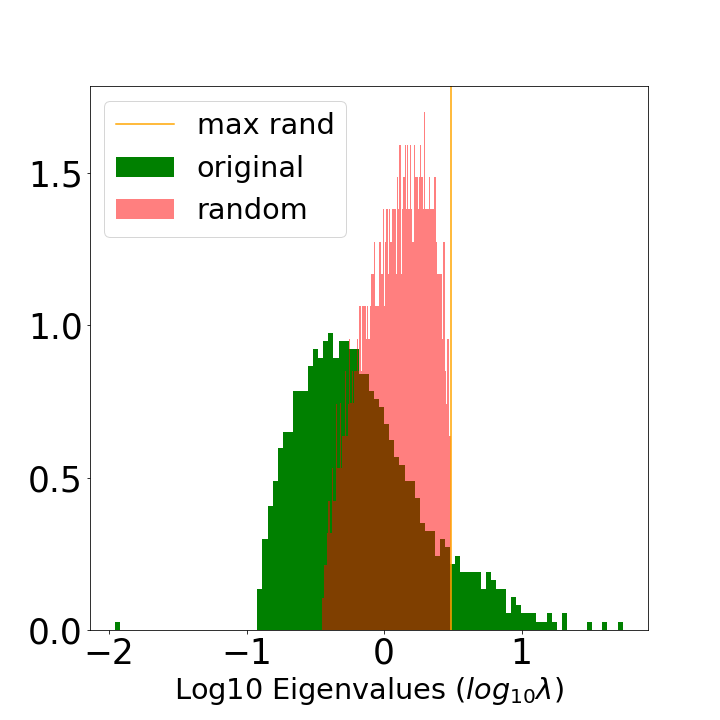
\includegraphics[width=7cm]{./img/shape-scale-a.png}
      \label{fig:scale-shape-a}
    }                               
    \subfigure[ESD with \CorrelationTrap]{                   
      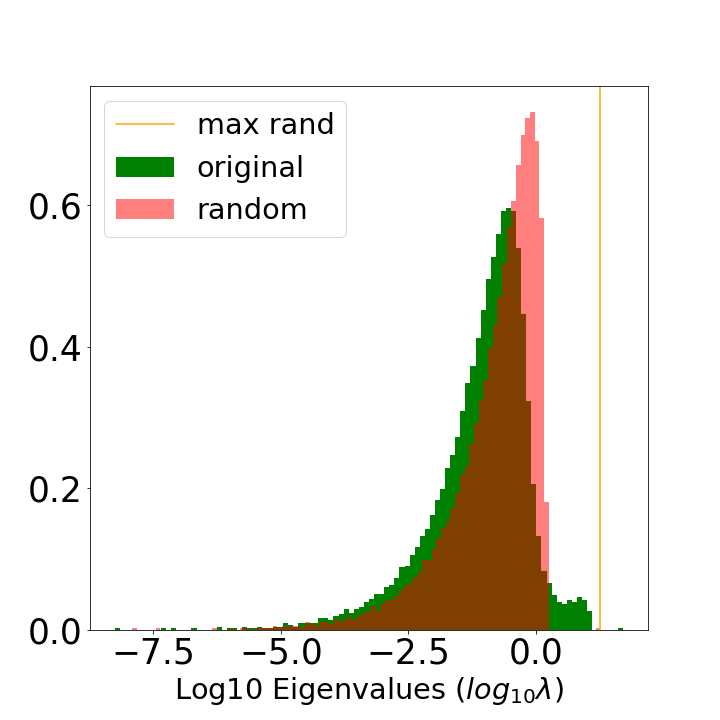
\includegraphics[width=7cm]{./img/shape-scale-b.png}
      \label{fig:scale-shape-b}                           
    }                                                                                                                            
    \caption{Comparison of a well-formed, Heavy-Tailed ESD (a) to one with a Correlation Trap (b), in the VGG16 model (FC2 layer)}
  \label{fig:scale-shape}                                                                                                      
\end{figure}

See Figure~\ref{fig:scale-shape-a}, which displays the (log)-ESD of a \Typical SOTA NN layer $\mathbf{X}$ (green), i.e., on a log-linear scale, along with the (log)-ESD of that layer after randomizing it element-wise (red).
The two ESDs differ substantially:
the ESD of the original weight matrix  $\mathbf{W}$ (green) is very HT, whereas 
the ESD of the randomized weight matrix  $\mathbf{W}^{rand}$ (red) is an MP (and as predicted by the MP \RMT).
The orange line corresponds to the maximum eigenvalue of the randomized ESD.
Note that it is at the MP bulk edge of the red plot, indicating that this ESD is not affected by unusually large elements or other weight anomalies.
Here, we say that the ESD of $\mathbf{X}$ is HT, and that $\mathbf{W}$ is not HT element-wise.
\HTSR says this layer is well trained.

Contrast this with Figure~\ref{fig:scale-shape-b}, which displays the (log)-ESD of a NN layer with a \CorrelationTrap.
The ESD of $\mathbf{X}$ (green) is weakly HT, but it looks nothing like the ESD in Figure~\ref{fig:scale-shape-a}.
In fact, it looks very much like the ESD of the randomized weight matrix  $\mathbf{W}^{rand}$ (red), except for a small shelf on the right. 
The orange line again corresponds to the maximum eigenvalue of the randomized ESD, and this is just past this shelf.
Relative to the randomized ESD, this line depicts (an) unusually large element(s)---or, equivalently, a rank-1 perturbation of $\mathbf{W}^{rand}$.
By a \CorrelationTrap, we mean that some anomaly in the elements of $\mathbf{W}$ tends to ``trap'' the ESD of $\mathbf{X}$, concentrating the correlations in $\mathbf{X}$ into the small shelf of density around the orange line. 
\HTSR says this layer is not well-trained because it does not have a good PL fit.

%We will see, below in Section~\ref{sxn:empirical}, that we can induce a \CorrelationTrap by shrinking the batch size, and that this is associated with a degradation in model performance (%as well as spuriously low PL exponent $\alpha$). 


%\paragraph{Correcting for \SCALE Anomalies with \ALPHAHAT}
%\subsubsection{Correcting for Scale Anomalies with \ALPHAHAT}

%\nred{repetitive ?}
%  \CorrelationTraps are a kind of \SCALE anamoly;by this we mean when the layer weight matrix $\mathbf{W}$
%  and/or the randomized  $\mathbf{W}^{rand}$ has one or more unusually large eigenvalues $\lambda$.
%  In the case of a scale anamoly, the simple PL \ALPHA metric may not correlate well with the test accuracy or other measures
%  of model quality because such scale anomalies may make it difficult to get a good PL fit of $\alpha$.
%  In some very hard cases, the layer ESD $\rho_{emp}(\lambda)$ may be significantly deformed from a well
%  behaved PL or TPL distribution (as in Fig.~\ref{fig:scale-shape-b}.  In these cases, the \ALPHAHAT
%  metric can frequently compensate.  This is seen in Section~\ref{sxn:empirical} \nred{see github issue 46}

 





\subsubsection{Over-Regularization}
\label{sxn:underfitting}

%\michael{Is the idea that this section parallels Section~\ref{sxn:Traps}, in that both describe non-\Ideal learning?  If so, we need to refine.  Are we saying that the primarily way $\alpha<2$ is when one layer is compensating for another.  }

The second way we identify $\mathbf{W}$ as \ATypical is when it has an anomalously large variance $(\sigma^2(\WMAT))$.
\michaeladdressed{Variance of what.}

The \SETOL theory -- a single-layer theory of learning -- casts the training 
of a NN layer in terms of how the correlations concentrate into the layer  \EffectiveCorrelationSpace (\ECS),
and becomes exact when the \TRACELOG condition is satisfied.
Analogously, the \HTSR theory -- a single layer \Phenomenology of learning -- casts training
of an N layer by fitting its ESD to a PL, and noting that the PL exponent $\alpha$ measures
the amount of implicit regularization in the layer.
Comparing the two approaches, we see that smaller $\alpha$ corresponds to the correlations
concentrating into a low-rank~\ECS.  In general, and likewise, the more the weight matrix
correlations concentrate  into a low-rank~\ECS, the better the layer has been regularized.
A natural question arises then, namely, can a layer be \emph{\OverRegularized} and
can we detect this?
and in large,
Empirically, we do indeed observe that over the course of training, $\alpha$ decreases, (See Figure~\ref{fig:mlp3-FC1-alpha-overloaded} 
(a), Section~\ref{sxn:hysteresis_effect},) and that the models predictions are concentrated into the~\ECS, 
(See Section~\ref{sxn:empirical-effective_corr_space}). Thus, we also interpret $\alpha$ and~\ECS concentration to be 
measures of learning itself, meaning that NNs are self-regularizing~\cite{MM18_TR_JMLRversion}.

Importantly, however, the \HTSR \Phenomenology indicates that \ALPHA usually lies in the Fat-Tailed Universality class,
such that $\alpha\in [2,6]$.  When $\alpha <2$, the ESD is Very Heavy Tailed (VHT), and, also,
this indicates that $\mathbf{W}$ has an anomalously large variance.  That is,  $\mathbf{W}$ is  \ATypical.
Occasionally, but very infrequently, we do observe $\alpha<2$, and in large, production quality models
(like Llama).
Interestingly, we also observe that, frequently, when the \HTSR $\alpha<2$, the \SETOL \TRACELOG
condition holds fairly well.  This is further explored in Section~\ref{sxn:empirical}

We have applied the \WW tool to have examined dozens
of modern, very large NNs; of particular interest are the so-called Large Language Models
(LLMs) that have revolutionized the field of AI.  To that end, in Figure.~\ref{fig:falcon_vs_llama},
we present the \WW layer \ALPHA metrics for the Falcon-40b and the Llama-65b LLMs.
\footnote{Similar results are found for the larger, more modern Llama models,
and can be found on the ~\WW website\cite{WW}}

\begin{figure}[ht!]
    \centering
    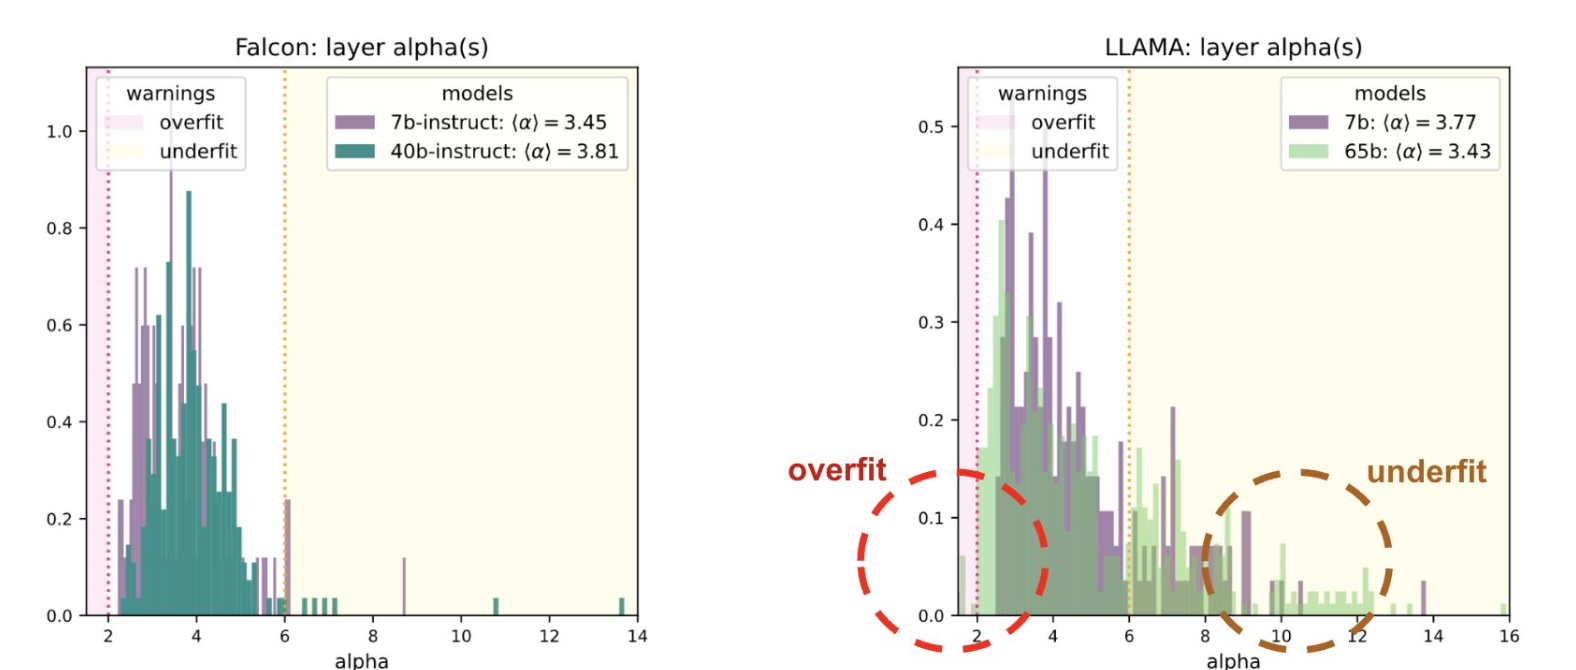
\includegraphics[width=15cm]{./img/falcon_vs_llama.png}
    \caption{Falcon vs Llama}
   \label{fig:falcon_vs_llama}
\end{figure}

For the Falcon-40b model, all of the layer \ALPHA range between $\alpha\in[2,6]$,
and therefore lie in the Fat-Tailed Universality class (in Table~\ref{tab:Uclass})
and are well-fit.
In contrast, looking at the Llama-40b layer \ALPHA, very many have $\alpha>6$,
indicating these layers are under-fit, and while a few have $\alpha <2$, suggesting
these are over-fit.  Finally, there are more layers with $\alpha~\sim2$ in Llama-65
vs Falcon-40b.

The observations on Llama-2 suggest that the layers with $\alpha\le 2$
are compensating for the layers with $\alpha>6$, and yielding suboptimal
performance for the Llama-65b architecture.
Based on these observations, we hypothesize that, in a multi-layer-perceptron (MLP),
when one layer does not or can not learn, then other layers will
have to compensate, and will be overloaded with the training data,
leading to $\alpha<2$, and even the \TRACELOG condition $\Delta \lambda_{min} < 0$.

%In Section~\ref{sxn:empirical} below, we will test this hypothesis in a 3-layer MLP model
%(MLP3), trained on MNIST, but only training 1 (FC1 or FC2), while keeping the other 2 frozen.
%In this way, we can simulate the situation seen above in the Llama-65b model,
%and observe the formation of a VHT ESD in the layer being trained.

%Additionally, as argued below, we conjecture that when $\alpha<2$, the model
%enters a kind-of glassy meta-stable phase, similar to the kinds of phases
%predicted by classic \STATMECH theories of learning.  A
%\nred{explain idea that VHT is \ATypical}

%We will explore how far we can push this analogy in our experiments to stress test the \SETOL approach.
%In particular, we will see effects reminiscent of a glassy system-the slowing down
%of the dynamics (in Sections~\ref{sxn:fc1})
%and a kind of hysteresis (Section~\ref{sxn:hysteresis_effect})

In Section~\ref{sxn:hysteresis_effect}, we will test this hypothesis.
By reducing the trainable parameters in a small MLP, we can simulate the situation seen above in the Llama-65b model,
and observe the formation of a Very Heavy Tailed (VHT) ESD in the dominating layer weight matrix.
Overloading results from having too few parameters for the complexity of the task. Adding more data increases 
the load up to the total complexity of the task itself.
%\st{Adding noisy labels increases the load up to the capacity of the a}

Moreover, we will also argue that in our experiments,
the model enters a kind of glassy meta-stable  phase, similar to the kinds of phases predicted by
classic \STATMECH theories of learning~\cite{SST92}
(described below).
Section~\ref{sxn:hysteresis_effect} will explore how far we can push the analogy of glassy systems in our experiments to 
stress test the \SETOL approach. In particular, we will see effects such as the slowing down of its dynamics, leading to a kind 
of hysteresis, specific to the under-parameterized regime.







\newpage
\section{Statistical Mechanics of Generalization (\SMOG)}
\label{sxn:SMOG_main}

In this section, we review \STATMECH: 
both to understand how it is usually applied in \StatisticalMechanicsOfGeneralization (\SMOG) theory; 
and to understand how our \SemiEmpirical approach in \SETOL is similar to and different from the traditional approach.
The goal is to obtain an expression for the \GeneralizationAccuracy (or \ModelQuality $\Q^{ST}$) for the
classic \StudentTeacher (ST) model of the Linear \Perceptron (in the AA, and at high-T),
as described in \cite{SST90,SST92}.
In Section~\ref{sxn:matgen}, we will generalize this to a \LayerQuality metric, $\Q$, for a layer in a general Multi-Layer Perceptron (MLP),
i.e., $\Q^{ST}\rightarrow\Q$, so that $\Q$ can then be expressed in terms of the ESD of the NN layer.

\paragraph{Outline.}
Here is an outline of this section.
\begin{enumerate}[label=4.\arabic*]
\item
  \textbf{Traditional Approaches to the \SMOG}
  In Section~\ref{sxn:trad_smog}, we explain the mapping from the \STATMECH theory of disordered systems
    to the \STATMECH theory of NN learning (\SMOG); and, additionally, how our \SemiEmpirical approach
    is similar to and different from the traditional approach.

  \item
      \textbf{Mathematical Preliminaries}
    In Section~\ref{sxn:mathP}, we review the mathematical details of \STATMECH, providing definitions
      and detailed derivations of quantities and expressions necessary later.  

    \item
        \textbf{Student-Teacher Model:}
      In Section~\ref{sxn:SMOG_main-student_teacher}, we discuss the setup of the \StudentTeacher (ST) model
    as a general means to estimate the \AverageGeneralizationError empirically.  

  \item
      \textbf{Generalization Gap vs. Model Quality}
    In Section~\ref{sxn:SMOG_main-model_quality}, we briefly highlight the differences between the \STATMECH model
    of the \GeneralizationAccuracy and the ST model for the \GeneralizationGap.

  \item
      \textbf{Bad Training Data and the Spin Glass Phase}
    In Section~\ref{sxn:SMOG_main-spin_glass}, we describe the qualitative aspects of spin-glass theory
    and its implications for the ST model.

  \item
      \textbf{Average Generalization Error $(\AVGSTGE)$}
    In Section~\ref{sxn:SMOG_main-st_av}, we derive the (new) result for the
    ST \ModelQuality, $\Q^{ST}$, using the setup of the classic (ST) model for the
    \GeneralizationError (and accuracy) of the \Perceptron (in the AA, and at high-T).
\end{enumerate}

\noindent
Additional information can be found in the Appendix.
\begin{enumerate}[label=A.\arabic*]
\item
  \textbf{Symbols and Equations}
  In Section~\ref{sxn:appendix_A}, we summarize the important symbols and key results,
         including the dimensions of the vectors and matrices, the different notations for the energies,
         and the key equations necessary here and later.
   \item
   \textbf{Summary of the \SMOG}
         In Section~\ref{sxn:summary_sst92}, we provide a more detailed analysis of the results we derive in Section~\ref{sxn:SMOG_main-st_av}.
         In particular, in Section~\ref{app:st-gen-err-annealed-ham}, we repeat the derivations of the ST \GeneralizationError $\AVGSTGE$ and related quantities (from Section~\ref{sxn:mathP}),
         using more concrete notation to align with \cite{SST90, SST92}; and
         in Section~\ref{sxn:appendix_Gan}, we use this to derive the matrix-generalization of the ST \EffectivePotential $\EPSLR$ (as well as the normalization for the weight matrices, necessary for later).
\end{enumerate}

%\subsection{Traditional Approaches to the \SMOG} 
\subsection{\STATMECH: the \SMOG approach and the \SETOL approach} 

\label{sxn:trad_smog}

In this subsection, we review the basic \STATMECH setup necessary to understand \SMOG theory as well as \SETOL.
This theory was developed in the 1980s and 1990s~\cite{SST90,SST92,Gar85,Gar88,engel2001statistical}. 


\begin{table}[t] %[h!]
\centering
%\begin{center}
\renewcommand{\arraystretch}{1.15} % Increases row height
\begin{tabular}{c|c}
  \textbf{Statistical Physics} & \textbf{Neural Network Learning}                      \\ \hline
  Gaussian field variables     & Gaussian i.i.d data  $\NDXI\in\mathcal{D}$            \\ \hline
  State Configuration          & Trained / Learned weights $\WVEC$                     \\ \hline
  State Energy Difference      & Training and Generalization Errors  $\AVGTE, \AVGGE$  \\ \hline
  Temperature                  & Amount of stochasticity present during training $T$       \\ \hline
  \AnnealedApproximation       & Average over the data first                          \\ \hline
  \ThermalAverage              & Expectation w.r.t. the distribution of trained models \\ \hline
  \FreeEnergy                  & Generating function for the error(s) $F$             \\ \hline
\end{tabular}
%\end{center}
\caption{Mapping between states and energies of a physical system and parameters of the learning process of a neural network.}
\label{table:statMech_to_NNs}
\end{table}


\begin{table}[t] %[h!]
\centering
%\begin{center}
\renewcommand{\arraystretch}{1.15} % Increases row height
\begin{tabular}{c|c}
  \textbf{SETOL Terminology} & \textbf{Explanation}                      \\ \hline
  \ModelQuality $\Q$          & \makecell{Generalization accuracy, \\in the AA and at high-T }      \\ \hline
  \LayerQuality $\Q$          & \makecell{Layer contribution to the accuracy, \\in the AA and at high-T}       \\ \hline
  \LayerQualitySquared $\QT$ &  \LayerQuality squared, used for technical reasons \\ \hline
  \Quality \GeneratingFunction $\Gamma_{\Q}, \Gamma_{\QT}$   & Generating function for quality    \\ \hline
  \AnnealedHamiltonian $H^{an}$                & \makecell{Energy function, \\for errors or accuracies}             \\ \hline
  \EffectiveHamiltonian $H^{eff}$     & \makecell{Exact energy function, \\but restriced to a low-rank subspace}      \\ \hline
\end{tabular}
%\end{center}
\caption{Additional terminology introduced for the \SETOL.  
  Notice that the \Quality \GeneratingFunction $\Gamma$ is simply one minus the \FreeEnergy, $\Gamma:=1-F$,
but it introduced because sign convention for the \FreeEnergy is always decreasing with the error.
  In contrast, we define the Hamiltonian in terms of the model error or accuracy, depending on the context.
  \michael{AWK.}
  }
\label{table:SETOL_terminology}
\end{table}


\paragraph{Traditional \SMOG theory.}
In traditional \SMOG theory, one maps the learning process of a NN to the states and energies of a physical system.
The mapping is given in Table~\ref{table:statMech_to_NNs}.
\SMOG theory models the SGD training of a \emph{\Perceptron}, on the data, $\NDX$, to learn the optimal weights, $\WVEC$, as a Langevin process.%
\footnote{Typically, we have no guarantee of the true equilibrium in a high‐dim nonconvex landscape; so,
when the \emph{\ThermodynamicLimit} exists,
the  Langevin process converges or relaxes to the thermodynamic equilibrium.}
The power of the \STATMECH approach comes from the fact that the core concept of \ThermalAverages corresponds to taking the expectation of a given quantity only \emph{over the set of trained models}, as opposed to uniformly over all possible models (or, in a worst-case sense, over all possible models in a model class).
This capability is particularly compelling in light of the \STATMECH capacity to characterize disordered 
systems with complex non-convex energy landscape (which can even be \emph{\Glassy}, characterized by a
highly non-convex landscape~\cite{SST92, STS90, engel2001statistical},
and recognized classically by a slowing down of the training dynamics~\cite{gutfreund1985spin}).
Thus, concepts such as training and \GeneralizationError arise naturally from integrals that are familiar to \STATMECH; 
and theoretical quantities such as Load, Temperature, and \FreeEnergy also map onto useful and relevant concepts~\cite{MM17_TR}. 
The \FreeEnergy is of particular interest because it can be used as a generating function to obtain the desired \GeneralizationError and/or accuracy.
We wish to understand how to compute the associated thermodynamic quantities such as the expected value of the
various forms of the \AverageGeneralizationError $(\AVGGE)$, \PartitionFunction $(Z)$, and the
\FreeEnergy $(F)$ and other \GeneratingFunctions~$(\Gamma)$.


\charles{TODO: discuss mean field theory, saddle points, replicas, etc.} 
\michael{Certainly not~here.}
\charles{A good introduction discusses the themes in a section}
\michaeladdressed{@charles: Can we just cange ``Generalization Accuracy'' to ``Model Quality'' and ``Model Accuracy'' since I think that will help to minimize confusion.  We should define what precisely is Model Quality and new notions.}

\paragraph{The \StudentTeacher model.}
\charles{@michael?  Removing for now ; we should discuss :
XXX. PUT TWO OR THREE SENTENCES ON THE BASIC STUDENT SETUP; START WITH THE FOLLOWING AND REFINE.
For simplicity, let's consider the classification of the elements of some input space $X$ into one of two classes, $\{0,1\}$.
There is a \emph{target rule}, $T$, which is one particular mapping of the input space into the set of classes, as well as a \emph{hypothesis space}, $\mathcal{F}$, which consists  of the available mappings $f$ used to approximate the target $T$.
The set $\mathcal{F}$ could, e.g., consist of NNs with a given structure.
Given this setup, the problem of learning from examples is the following: on the basis of the classification determined by the target rule $T$ for the elements of a subset $\mathcal{X} \subset X$, which is the \emph{training set}, select an element of $\mathcal{F}$ and evaluate how well that element approximates $T$ on the complete input space $X$.
One can think of the target rule $T$ as being a \emph{teacher}, and the goal of the \emph{student} is to approximate the teacher as well as possible.
The \emph{generalization error} $\varepsilon$ is the probability of disagreement between the student/hypothesis and teacher/target on a randomly chosen subset of $X$.
XXX. OLD STUFF VECTORS.
XXX. NEW STUFF MATRICES.}

%To express these integrals, the \SMOG approach models both Students $S$ and Teachers $T$ as \emph{weight vectors},
We seek to compute and/or estimate the  \AverageGeneralizationAccuracy for a \emph{fixed} \Teacher Perceptron $T$
by averaging over an ensemble of \Student $S$ \Perceptrons, in the \AnnealedApproximation (AA), and at
\HighTemperature (high-T); we call this ST \ModelQuality, and denote it $\Q^{ST}$.
We will then, later, in Section~\ref{sxn:matgen}, we generalize $\Q^{ST}$ to an
arbitrary layer in \MultiLayerPerceptron, giving a \LayerQuality, i.e., $\Q^{ST}\rightarrow\Q$.
This formulation of the ST problem is different than the classic approach  because one
usually does not fix the \Teacher but, instead,
averages over all \Teacher vectors $\TVEC$~\cite{SST92,engel2001statistical}.
This is one of many ways that distinguishes the current approach from previous work.
Because of this, we present both a pedagogic derivation of $\Q^{ST}$
(for a general NN in Section~\ref{sxn:mathP}, and for the ST model specifically
in the Appendix, Section~\ref{sxn:summary_sst92}),
and we provide a more heuristic approach in Section~\ref{sxn:SMOG_main-st_av}, assuming
the AA and high-T at all times.


\paragraph{Towards a \SemiEmpirical Theory.}
In the \SETOL approach to \STATMECH, we want a matrix generalization of the ST \ModelQuality, $\Q^{ST}$, for a single \LayerQuality
$\Q\sim\Q^{NN}_{L}$ in an arbitrary \MultiLayerPerceptron (MLP).
This matrix generalization is a relatively straightforward extension of the classical (i.e., for a vector \Teacher) \SMOG ST \ModelQuality (but our \SETOL approach will use it in a conceptually new way).
%
In our matrix generalization, the \Teacher vector $\TVEC$ is replaced by a \Teacher matrix $\TMAT$ (i.e., $\TVEC\rightarrow\TMAT$); 
and, in our \SETOL approach, $\TMAT$ will be an actual (pre-)trained NN weight matrix (i.e., $\TMAT=\WMAT$). 
Importantly, this matrix $\WMAT$ is neither a Gaussian Random Matrix, nor is it obtained from Gaussian i.i.d training data.
As such, for our \SETOL theory, we seek an expression that can be parameterized by the \Teacher, and in particular by the ESD of the \Teacher.
This is what makes the basic method \SemiEmpirical: even though we do not know the form of the \Teacher,
we make a modeling assumption that the  \Teacher has the same limiting spectral distribution as the \Student, 
and hence the same PL fit parameter $\alpha$. 
This is all done with the understanding that later we will augment
(and hopefully ``correct'') our mathematical formulations with 
phenomenological parameters fit from experimental data.
To make the \SemiEmpirical method a \SemiEmpirical \emph{Theory}, 
we not only seek to parameterize our model; but 
we also try to understand 
how to derive \HTSR empirical metrics, such as $\ALPHA$ and $\ALPHAHAT$,
how they arise from this formalism, 
how they are related to the correlations in the data, and 
why they are transferable and exhibit \Universality.
This gives what we call a \SemiEmpirical \emph{Theory}.

\subsection{Mathematical Preliminaries of Statistical Mechanics}
\label{sxn:mathP}

%MM% We will compare and contrast the several types of energies and averages we will encounter:
%MM% Thermal Averages (over the weights $\WVEC$),
%MM% Sample Averages (over the data $\XVEC$),
%MM% and \FreeEnergies and \GeneratingFunctions.
%MM% We will define the different averages, 
%MM% show how they are related to each other under the  \AnnealedApproximation (AA) and in the \HighTemperature (High-T) limit,
%MM% and explain how and when may use the (overloaded) \BraKet notation $\langle \cdots \rangle$ for the different averages.
%MM% We will then show how to compute the average training and test/generalization errors $\AVGTE, \AVGGE$
%MM% using the \FreeEnergy as a \GeneratingFunction, and how they are related to each other
%MM% in the AA and the High-T limit.  We  briefly define \Replicaa Averages and
%MM% also the \SaddlePointApproximation (SPA).
%MM% Finally, we review how to express the \FreeEnergy
%MM% as a matrix-generalized \ThermalAverage over random matrices, called an HCIZ integral.

\paragraph{SubSection Roadmap}
Briefly, in the following subsection,
we start by defining an arbitrary NN model, with weights $(\WVEC)$.
Then, we explain the difference between using real-world $(\XVEC)$ and random data $(\XI)$.
This lets us define an energy error function, $\DETOP$,
the error the NN makes on the data.
We then explain how to take different kinds of \emph{\Thermodynamic} averages of the data,
including \emph{Sample} and \emph{\ThermalAverages} and the implications,
and the difference between computing errors and accuracies.
Next, we define the \emph{FreeEnergy} $(F)$ for the error(s), and the \emph{GeneratingFunction} $(\Gamma)$
for the accuracy and/or quality.
From here, we explain the \emph{AnnealedApproximation} (AA) and
how to define the  \emph{\AnnealedHamiltonian}, $\GAN$, a crucial expression
that will be the starting point later for our matrix model.
In the AA, $\GAN$ simplies to  $\HANHT=\EPSLw$, where $\EPSLw$ is an \EffectivePotential
that depends only on the weights $\WVEC$.
Likewise, we can define the \SelfOverlap, $\ETAw:=1-\EPSLw$, which is useful for
obtaining the \Quality.
We show how to obtain the \emph{Average Training and Generalization Errors} $\AVGTE$, $\AVGGE$
using the \STATMECH formalism, which defines them in terms of partial derivatives of the \FreeEnergy $(F)$.
Doing this, we show that in the AA and at high-T they are equivalent,
$[\AVGSTTE]^{an,hT}=[\AVGSTGE]^{an,hT}$,
and can both be expressed as a \ThermalAverage over all Students, as a function 
of the \Teacher, as $[\AVGSTGE]^{an,hT}=\THRMAVG{\GANHTR}=\THRMAVG{\EPSL(R)}$.
Note that these averages are obtained by using the \FreeEnergy as a \GeneratingFunction.
We then explain how to obtain the \ModelQuality  as  partial derivatives of a
\emph{\GeneratingFunction} $(\Gamma_{\Q})$.
We then discuss the more advanced techniques, the
\emph{\LargeN Approxmation} and the \emph{SaddlePointApproximation} (SPA),
which will be used extensively later.
Finally, we introduce  HCIZ integrals, which will be necessary to evaluate the matrix-generalized
form of $\Gamma_{\Q}$ to obtain the final result.
%\footnote{This assumes that agreement of \Student and \Teacher predictions will follow from overlap of weight vectors --- as it 
%surely does in the \emph{\LinearPerceptron} case, and does with high probability under Lipschitz 
%smoothness~\cite{neyshabur18_TR}. 
%\michaeladdressed{@charles: Im not sure what this is saying.}\charles{YOU WROTE THIS!}
%}
\michael{@charles: What precisely is Accuracy versus Quality?}
\charles{@michael: We have discusses this multiple times. }
%We also degfine  write an expression for the Average \GeneralizationAccuracy,
%$1-\AVGSTGE$, which we call the \ModelQuality.
\michaeladdressed{This last sentence is an exaple of one where the phrasing is a little unclear.  I think we can mention \ModelQuality, but it's not clear if this is from SST or something we introduce, etc.  So, it's unclear later when we use it without a clear definition, etc., in the vector or matrix case.  Probably it's best just to either remove a sentence like that here (if SST did not have it, since here we are describing the past), or have a footnote saying that we will use the \GeneralizationAccuracy they used, but in a different way by considering one-minus it, and then have an explicit pointer to where we define it.}

In this subsection, we will compare and contrast several types of averages and energies we will encounter. 
\michaeladdressed{@charles: we can remove the itemize block later and just keep the text, I have it this way for now just to make sure we get every subsubsection, etc.}
\charles{I actually prefer the itemized block; if the journal does not like it then it can be changed}
%
\red{THIS IS OUT OF SYNC.}


\begin{enumerate}[label=4.2.\arabic*]
\item
  \textbf{Setup.}
  In Section~\ref{sxn:mathP_setup}, 
we will start by describing the basic setup of the problem, including the distinction between the actual training process and how we model the training process.

 \item
  \textbf{Sample Averages, Expected Values, and Thermal Averages.}
In Section~\ref{sxn:mathP_averages}, 
we will describe Thermal Averages (over the weights $\WVEC$) and Sample Averages (over the data $\XVEC$)---in particular, under the \AnnealedApproximation (AA) and in the \HighTemperature (High-T) limit---showing how they relate to each other and to the notion of \Replica Averages.
%
\item
  \textbf{Free Energies and \GeneratingFunctions.} 
In Section~\ref{sxn:mathP_free_energies}, 
we will make a connection between these different averaging notions and \FreeEnergies and \GeneratingFunctions, showing how they relate to each other.
%

\item
  \textbf{The Annealed Approximation (AA) and the High-Temperature Approximation (high-T).}
  In Section~\ref{sxn:mathP_annealed}, we explain the \AnnealedApproximation, the \HighTemperature approximation,
  and the Thermodynamic \LargeN limit and the Saddle Point Approximation (SPA).
  We also introduce the \Quality \GeneratingFunction $\Gamma_{\Q}$
    \michaeladdressed{@charles: nik: we have an extra space there due to the xpace in the macro; if there are only two generating functions, then maybe just list both.}
%
  \item
    \textbf{Average Training and Generalization Errors and their \GeneratingFunctions.}
  In Section~\ref{sxn:mathP_errors}, we will show how to compute the Average Training and Test/Generalization Errors $\AVGTE, \AVGGE$
using the \FreeEnergy as a \GeneratingFunction, and how these errors are related to each other in the AA and High-T limit. 
We will also make connections with the \SaddlePointApproximation (SPA).
%
\item 
  \textbf{The Thermodynamic \LargeN limit and the Saddle Point Approximation (SPA).}
  In Section~\ref{sxn:largeN_and_SPA}, we discuss the \LargeN \ThermodynamicLimit and the \SaddlePointApproximation (SPA).
  We also the introduce concept of \SelfAveraging.
%
 \item
  \textbf{HCIZ Integrals.}
Finally, in Section~\ref{sxn:mathP_hciz}, we will describe how to express the \FreeEnergy as a matrix-generalized \ThermalAverage over random matrices, called an HCIZ integral.
\end{enumerate}
The various symbols and other important results are summarized in the Appendix~\ref{sxn:appendix_A}


\subsubsection{Setup}
\label{sxn:mathP_setup}

A basic issue in formulating \SETOL is that one typically trains one large (expensive) NN, i.e., one does not split the data into training and testing sets.
Thus, we want a methodology to approximate quantities such as the generalization error or generalization accuracy that does not rely on traditional train-test splitting methods.
\michaelB{Q: how does this lack of using training/testing split relate to that we ignore the $y$ below and/or that we are actually getting a notion of quality/accuracy, rather than error (related to $\Gamma$ versus $F$).}
To accomplish this, we idealize the empirical data distribution as Gaussian fields, and we will use \STATMECH to construct quantities (basically, free energies or generating functions) so that we can compute training/testing errors by taking appropriate derivatives of these quantities.

In more detail, we imagine training a NN on $\ND$ training data instances, $\XVEC_{\mu}$, which are $m$-dimensional vectors,
with labels $y_{\mu}$, chosen from a large but finite-size training data set $\ADD$.
The goal of training a perceptron (or, later, a NN) is to learn the $m$ weights of the vector $\WVEC$ (or, later, a weight matrix $\WMAT$) by minimizing a loss function $\mathcal{L}$. 
We want to approximate the actual network’s learning dynamics by an analytically tractable ensemble
so that we can then obtain 
analytic expressions for the \emph{\FreeEnergy} and \emph{\GeneratingFunction} we then use to compute
Thermodynamic averages such as the \emph{\AverageGeneralizationError} $(\AVGGE)$ and
\emph{\ModelQuality} $(\Q)$ (which is our approximation to the \emph{\AverageGeneralizationAccuracy}).


\begin{figure}[t] %[h] % [h] places the figure approximately here
    \centering
\resizebox{0.75\textwidth}{!}{
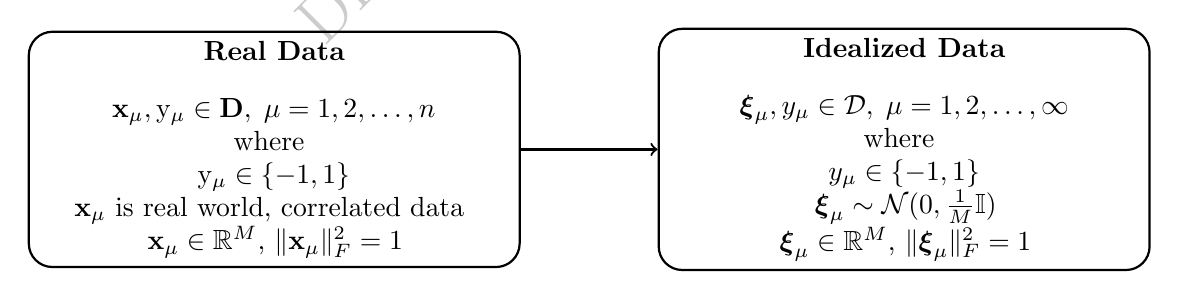
\begin{tikzpicture}[
     thick, % Line thickness
    rectnode/.style={rectangle, draw=black, thick, minimum width=6cm, minimum height=2.5cm, rounded corners=0.3cm}, % Rectangular node style with rounded corners
    -> % Arrow style
]

% Nodes with manual positioning
\node[rectnode] (realdata) at (0,0) {%
    \begin{minipage}{6cm}
        \centering
        \textbf{Real Data} \\
        \vspace{0.3cm}
        $\mathbf{x_\mu}, \mathrm{y}_\mu \in \mathbf{D},\;\mu=1, 2, \ldots, n$\\
        $\text{where }$ \\
        $\mathrm{y}_\mu \in \{-1, 1\}$ \\
        $\mathbf{x_\mu}\text{ is real world, correlated data }$ \\
        $\mathbf{x_\mu} \in \mathbb{R}^{M}$, $\Vert\mathbf{x_\mu}\Vert^{2}_{F}=1$
    \end{minipage}
};

\node[rectnode] (modeldata) at (8,0) {%
    \begin{minipage}{6cm}
        \centering
        \textbf{Idealized Data} \\
        \vspace{0.3cm}
        $\boldsymbol{\xi}_\mu, y_\mu \in \mathbf{\mathcal{D}},\;\mu=1, 2, \ldots, \infty$ \\
        $\text{where }$ \\
        $y_\mu \in \{-1, 1\}$ \\
        $\boldsymbol{\xi}_{\mu} \sim \mathcal{N}(0, \tfrac{1}{M} \mathbb{I})$ \\
        $\boldsymbol{\xi}_{\mu}\in \mathbb{R}^{M}$, $\Vert\boldsymbol{\xi}_{\mu}\Vert^{2}_{F}=1$
    \end{minipage}
};

% Arrow between the boxes
\draw[->] (realdata) -- (modeldata);

\end{tikzpicture}
}
\caption{Mapping from a fixed set of $n$
  real-world, correlated data instances $[\mathbf{x},\mathrm{y}]\in\mathbf{D}$
  to an uncorrelated, random model of idealized data   $[\boldsymbol{\xi}, y]\in\mathbf{\mathcal{D}}$, drawn from a Gaussian i.i.d. distribution.
}
    \label{fig:data_mapping}
\end{figure}




\paragraph{Counting Samples and Features.}
We let the number of training samples be $\ND$ and the dimension 
(i.e., number of features) for each sample be $m$.
% For simplicity, we also use $\ND$ (instead of $\ND$) and $M$ (instead of $m$), recognizing that 
% \emph{in later sections} $\ND$ and $M$ will refer to the dimensions 
% of a layer’s weight matrix (i.e., an $N \times M$ matrix). 
% We stress that here, in this subsection,  $n = N$ and $m = M$ only hold for our immediate analysis, 
% to avoid extra notation. 
When we move to matrix-based analyses, 
%we will revisit (and possibly distinguish) $\ND$ (layer input dimension) and $\ND$ (training-set size).
the input dimension $m$ will become $M$ and we will induce a new output dimension $\ND$, (the output dimension of a perceptron is $1$). Thus, the layer weight matrix $\WMAT$ has dimension $M\times N$.\footnote{To be more precise, $M$ is defined to be the lesser dimension of $\WMAT$ and $\ND$ the greater. For simplicity we assume that $M$ is always the input dimension and $\ND$ the output dimension. Under the assumptions of \SETOL, there is no loss of generality from doing this.} The number of data samples will remain $\ND$ throughout.
\begin{table}[H]
\centering
\begin{tabular}{l|l|l}
\toprule
 \textbf{Definition} & \textbf{Vector} & \textbf{Matrix} \\
\midrule
 Total number of data samples used in training. & $\ND$ & $\ND$ \\
 Number of features per training sample (Input dimension). & $m$ & $M$ \\
 Dimension of layer output (Output dimension)  & $1$ & $N$ \\
 Number of free parameters & $1$ & $N\times M$ \\
 Total number of degrees of freedom & $\ND\times 1$ & $\ND\times N\times M$ \\
\bottomrule
\end{tabular}
\caption{In the \emph{vector} model, lowercase $m$ is the dimension of the weight vector (total parameters), which is also the number of features per sample. In the vector case, there is one free parameter -- the overlap $R$ (or angle $\theta$) between student and teacher. In the \emph{matrix} model, uppercase $N$ and $M$ are the input and output dimensions of the weight matrix, resp., giving $N\times M$ free parameters.
The total number of degrees of freedom is the number of training examples $\ND$ times the number of free parameters.}
\label{tab:dim_notation}
\end{table}




\paragraph{Actual and Idealized Data and Energies.}

Consider having a large set $\ND$ of actual, real-world data, 
\begin{align}
  \label{eqn:x}
  \left( \XVEC_{\mu}, \MY_{\mu} \right) \in\ADD,\;\mu=1, \cdots, \ND,
\end{align}
where 
$\XVEC_{\mu}\in\mathbb{R}^{m}$ is an $m$-dimensional real vector, 
$\MY_{\mu}$ is a binary label taking values $\{-1,1\}$, and 
$\ADD$ denotes the finite-size dataset.
WLOG, we assume that $\XVEC_{\mu}$ is normalized such that the Frobenius norm squared is $\tfrac{1}{m}$:
\begin{equation}
  \label{eqn:XVEC_norm}
  \Vert\XVEC_{\mu}\Vert^{2}_{F} := \sum_{i=1}^{m} \XVEC_{\mu,i}^{2}=\tfrac{1}{m}
\end{equation}
\michaelB{Q: I just noticed that this means that the matrix $X$ consisting of all $m$ of those vectors has the scaling $\|X\|_F^2 = \frac{\ND}{m^2}$, which seems unusual; is that correct.}
We call $\XVEC^{\ND}$ an $\ND$-sized sample (of the training data instances $\XVEC$) from $\ADD$. 
% See below We may or may not specify the labels for this sample, depending on the context.

We define model errors
as a difference in energy $\DEL$ between the student's and teacher's output, since their outputs are a form of energy. Smaller energy differences correspond to smaller errors and therefore better models.
For example, for the mean-squared-error (MSE) loss, one has
\begin{align}
  \label{eqn:DEy}
  \DEL(\WVEC,\XVEC_{\mu},\MY_{\mu}):= (\MY_{\mu}-E_{NN}(\WVEC,\XVEC_{\mu}))^{2}  ,
\end{align}
where $E_{NN}(\WVEC,\XVEC_{\mu})$ is output prediction of the (student) NN, as in \EQN~\ref{eqn:dnn_energy}.

\michaeladdressed{To clarify: by modeling and ``real-worldexperiment, I think that what we are saying is that there is a training process on a particular dataset, and we are modeling the quality/generalization with the following, which includes replacing the real data with Gaussian data and the NN with a parameteric form that we will fit semi-empirically.}
\michael{@charles: we are going back and forth between Quality and Accuracy and various Errors; probably stick with errors, and introduce the Qualty/Accuracy in the subsubsection below.}
\charles{@michael: Eh?}

%There is a training process on a particular dataset, and we are modeling the \Quality (or generalization accuracy) with the following, which includes 
% To estimate quantities such as the generalization error or generalization accuracy, we will adopt an approach that involves
% replacing the real data with Gaussian data and
% the NN with a parametric model that we will fit with a \SemiEmpirical procedure (described later).
Following the usual \StatisticalMechanics trick, we idealize the inputs as independent Gaussian fields and the NN as a parametric model, in order to estimate quantities such as the generalization error or generalization accuracy. Moreover, just as the student's output is given by $E_{NN}(\WVEC,\XVEC_{\mu},\MY_{\mu})$, a core assumption of the \SETOL is that $\MY_{\mu}$ is also the output of a (realizable) Teacher NN. Thus, as we will see below, $E_{\mathcal{L}}$ is defined with reference to the Teacher weights, rather than the labels $\MY_{\mu}$, leading $\MY_{\mu}$ to be dropped from expressions of the error. This, and the fact that we will integrate out the data terms, are among the reasons why \SETOL is able to offer data-independent model Quality metrics. The replacement scheme is,
\begin{align}
\label{eqn:model_real_world_expt}
  \ADD \rightarrow \MDD,\;\;\XVEC_{\mu} \rightarrow \XImu,\;\;  \Ymu \rightarrow y_{\mu}  ,
\end{align}
%where we denote the model training and/or test data instances as $(\XI,y)$ 
such that
\begin{align}
    \label{eqn:xi}
  \left(\XI_{\mu}, y_{\mu} \right) \sim \MDD,\;\mu=1, \cdots, \infty  .
\end{align}
Here, $\XImu\in\mathbb{R}^{m}$ is a random vector %(i.e., an $m$-dimensional random variable),
sampled from an i.i.d $m$-dimensional joint distribution $\MDD$ of both the features $\XI_{\mu}$, which are Gaussian, and the labels $y_{\mu}$, which are binary Teacher NN outputs. Since we assume that the Teacher is fixed, and the labels are deterministically generated by it, $\MDD$ is effectively just the Gaussian feature distribution.
% and $y_{\mu}$ denotes the (binary) label and/or NN output.


\subsubsection{BraKets, Expected Values, and Thermal Averages}
\label{sxn:mathP_averages}
Given the setup from Section~\ref{sxn:mathP_setup},
%we will model the student's error as the average (difference in) energy, $\DETOPX$, over some $\ND$-size data set $\NDX$,
we can write the \TotalDataSampleError,
using an overloaded operator notation, as
\begin{align}
  \label{eqn:detopxy}
  \DETOPXY :=\sum_{\mu=1}^{\ND}\DEL(\WVEC,\XVEC_{\mu}, \MY_{\mu})  ,
\end{align}
where the boldface $\DETOP$ indicates this is a sum over the entire set of $\ND$ pairs $[\NDX, \MY^{\ND}]$.
% We should keep in mind that this depends on the specific set of $\ND$ data pairs $[(\XVEC_{\mu},\MY_{\mu})\in\ADD\;|\;\mu=1,\cdots,n]$, 
% although later we will model the labels $\MY_{\mu}$ as the output of another NN when describing the Student-Teacher model.
As mentioned above, we treat $\MY_{\mu}$ as a deterministic output of the Teacher model, meaning that
%for now, we will assume that the 
$\MY_{\mu}$ is \emph{implicit} in $\DEL$.
We will therefore drop the $\MY_{\mu}$ and $y^{\ND}$ symbols, 
and simply write this total error / energy difference as
\begin{align}
  \label{eqn:detox_FIXLATER}
  \DETOPX :=\sum_{\mu=1}^{\ND}\DEL(\WVEC,\XVEC_{\mu})  ,
\end{align}
which is now a function of the entire set of $\ND$ vectors $[\NDX]$.%
% (where the labels $\MY$ have been set implicitly).
\footnote{In the classic Student Teacher model, the labels  $\MY^{\ND}$ represent the Teacher outputs and are effectively treated as either uniform random variables to be averaged over later, or as the outputs of an optimal Teacher. In this work, the Teacher is fixed so we can drop the labels.}
This operator notation will prove useful later in Section~\ref{sxn:SMOG_main-st_av}
(see \EQN~\ref{eqn:DE_L}) and in Appendix~\ref{sxn:summary_sst92}.

We will not, however, work directly with samples and sample averages.
Instead, we will model them.
%%\michael{By that, I think we mean that it is hard to compute them, so we will model them with Gaussian random variables with a model with a parameter to fit semi-empirically to data; correct?}
%%\cformike{We discussed on the phone.  The idea is we compute the average as a derivative of a generating function that we know exactly, as opposed to say doing a monte carlo sample because the partition function $Z$ is intractable}
To that end, we need to estimate them 
%with a theoretical approach. For example, we can write the \TotalDataSampleError 
in terms of our random data variables $\XI$, written formally as
\begin{align}
\label{eqn:tdse}
\DETOPXI := \sum_{\mu=1}^{\ND}\DETmu ,
\end{align}
but to evaluate this we need to take an integral and/or \ExpectedValue over the data sample $\NDXIn$.

\paragraph{Expected Values.}

We need to compute various sums and integrals, sampling from a model $\MDD$ for the actual data distribution $\ADD$,  over $\ND$-sized data samples (or data sets), and also over distributions of weights ($\WVEC, \SVEC$) and weight matrices ($\WMAT, \SMAT, \AMAT, \cdots$).
This will frequently (but not always) be defined as more familiar \ExpectedValues.
We will denote \ExpectedValues using physics \BraKet notion.
Importantly, we use the term \ExpectedValue in the physics sense, and BraKets will denote an un-normalized sum or integral;
%notation denotes an inner product in a Hilbert space of functions;
when the quantity is to be normalized, we will denote the normalization explicitly.
For example, given a function $f(\XI)$, we write the BraKet integral as:
\begin{align}
 \label{eqn:EuT}
 \langle f(\XI) \rangle_{\XI}:=\int d\mu(\XI) f(\XI)  .
\end{align}
We would express an $\ND$-sized sample average over $f()$ as 
\begin{align}
    \label{eqn:EuT_normalized}
    \langle f(\NDXIn) \rangle_{\AVGNDXIn} :=& \frac{1}{\ND} \int d\mu(\NDXIn) f(\NDXIn) \nonumber \\
    =& \frac{1}{\ND} \left[\prod_{\mu=1}^{\ND} \int d\XI_{\mu}P(\XI_{\mu}) \right] \left[ \sum_{\mu=1}^{\ND}f(\XI_{\mu}) \right].
\end{align}
The BraKet $\langle\cdots\rangle_{\AVGNDXIn}$ denotes an integral over an $\ND$-sized sample of idealized
Gaussian-field data $\NDXIn$, with the convention that summation over $\ND$ points and normalization $\tfrac{1}{\ND}$
appears inside the \BraKet implicitly.
% If this integral is normalized properly, then this denotes the familiar \ExpectedValue $\mathbb{E}_{\XI}[f(\XI)]$.
% \michaelB{Clarify what is ``properly.?? Either remove that sentence, or say that is what \EQN~\ref{eqn:EuT_normalized} is.}
For example, consider how to compute \ExpectedValue of the \DataSampleError:
% That is, we want to model the average \DataSampleError using:
\begin{align}
  \label{eqn:Emap}
  \frac{1}{\ND}\DETOPX \xrightarrow{\text{Expected Value}} \langle \DETOPXI \rangle_{\AVGNDXIn}  , %= \DETOT = n \EPSLw.
\end{align}
In this case, we obtain:
\begin{align}
\nonumber
  \langle \DETOPXI\rangle_{\AVGNDXIn}
  :=  &\frac{1}{\ND}\int d\mu(\NDXIn) \DETOPXI \\ 
  = &
  \frac{1}{\ND}\int \left[ \prod_{\mu=1}^{\ND}d\XI_{\mu}P(\XI_{\mu})\right] \left[ \sum_{\mu=1}^{\ND}\DETmu \right] , \\ \nonumber
  = &
  \frac{1}{\ND}\sum_{\mu=1}^{\ND}\int d\XI_{\mu}P(\XI_{\mu})\DETmu  , 
    \label{eqn:average_data_sample_error}
\end{align}
where $P(\NDXIn)$ is a product of $\ND$ i.i.d. $m$-dimensional Gaussian distributions.
The subscript $\AVGNDXIn$ indicates this is an
\ExpectedValue of an average of an $\ND$-size \emph{sample} of ideal data, where the \ExpectedValue is taken over datasets, and the average is over data points within each sample. The third line follows because the $\ND$ samples are i.i.d.
(This is used in both Sections~\ref{sxn:SMOG_main} and~\ref{sxn:matgen}.)
Thus, the \red{implicit} normalization $\tfrac{1}{\ND}$ ensures the \BraKet is a proper \ExpectedValue of a sample average.
%The measure $d\mu(\NDXIn)$ signifies a single $\ND$ vector $\XI$, drawn from an $m$-dimensional idealized Gaussian distribution.
A subscript $\XI$ on the Ket as $\langle\cdots\rangle_{\XI}$ would represent an integral over potential data points, not an average of a data sample (i.e., there would be no $1/\ND$ prefactor).
% \michaeladdressed{@charles: clarify; that is $\ND$ vectors in $\mathbb{R}^{M}$ that are element-wise i.i.d. Gaussian?}
%%\michael{Where we are using $M$ and $\ND$ rather than $m$ and $\ND$; is that a typo, or what should it be.}
%%\cformike{I use $n,m$ in this section, $\ND$, $M$ elsewhere since they can mean different things when we generalize to a layer.  We can fix if its too confusion, or maybe just explain above.}
%

\paragraph{\SizeExtensivity and \SizeIntensivity}
A key requirement for the \ThermodynamicLimit in \STATMECH is \emph{\SizeExtensivity}:
that physically meaningful quantities (i.e, total energies and free energies)
scale linearly with the system size, $\ND$ (or $N$, below).
Extensive quantities scale with system size, intensive ones do not.
Along with this, Thermodynamic average quantities should be \emph{\SizeIntensive},
meaning that they remain independent of $\ND$ (or $N$) as the system size increases.
In our setting, \SizeExtensivity and \SizeIntensivity underpin the so-called \LargeN limit,
ensuring that macroscopic observables become independent of
microscopic fluctuations.

As an example of \SizeExtensivity and \SizeIntensivity, 
we write the \ExpectedValue (i.e., the data-average) of \DataSampleError $\DETOPXI$ (\EQN~\ref{eqn:average_data_sample_error})
in the \LargeN limit as
\begin{align}
  \lim_{n\gg 1} 
  \langle \DETOPXI\rangle_{\AVGNDXIn}=
  \lim_{n\gg 1}\frac{1}{\ND}
\int \prod_{\mu=1}^{\ND}d\XI_{\mu}P(\NDXIn)
  \sum_{\mu=1}^{\ND}\DEL(\WVEC,\XI_{\mu}) .
\end{align}
Here, the notation $(n \gg 1)$ means $\ND$ grows arbitrarily large, but is not necessarily
at the limit point $(n=\infty)$.
The \TotalDataSampleError $\DETOPXI$ is \SizeExtensive, whereas the
average $\langle\DETOPXI\rangle_{\AVGNDXIn}$ is \SizeIntensive.
This limit will be implicit later when taking a \SaddlePointApproximation (see below).
\footnote{As we are working within a ``physics-level of rigor, we take some liberties in evaluating these \LargeN limits; and we leave the formal proofs for future work. \michael{This comment should be in the intro, not in a footnote here.  Move later, since I don't have the token for the intro for now. } }
\nred{This is a little weird to have the square on this and ask it to be size extensive.  We should at least comment on this  See also SST92  eqn 2.1}

The data-averaged error  $\langle \DETOPXI \rangle_{\AVGNDXIn}$ will appear frequently below.
For convenience and for compatibility with \cite{SST92}, we denote it using the symbol $\EPSLw$:
\begin{align}
 \label{eqn:epsl}
 \EPSLw:=\lim_{n\gg 1}  \langle \DETOPXI \rangle_{\AVGNDXIn} \quad \text{(\SizeIntensive)}.
\end{align}
\michaelB{Q: Why do we not have the $\lim_{n\gg 1}$ notation there?}
where, by our normalization here, $\EPSLw \in [0,1]$.
\michaelB{Q: Where does it follow from that $\EPSLw \le 1$?  And we we need that anywhere?  (Below it follows when we specialize to L2, etc., but I mean more generally, which is where we are here.)}
The symbol $\EPSLw$ is our theoretical estimate of the sample average $\DETOPXI$ (\EQN~\ref{eqn:detox}),
well-defined for any $\ND$.
We also call $\EPSLw$ the \emph{\EffectivePotential}, which will be made clear below.

It is also convenient to write \emph{\TotalEffectivePotential} as an Energy, 
\begin{align}
 \label{eqn:detox}
 \DETOT := \ND\EPSLw\quad \text{(\SizeExtensive)}.
\end{align}
This will only be useful when the \ThermodynamicLimit exists, and this
can be reasonably expected for the \AnnealedApproximation (AA),
which is the regime in which \SETOL will be developed.% 
\footnote{We should note that, while our model training and generalization errors are always expressed energies, anenergy is not necessarily a model error. }


\paragraph{From Errors to Accuracies: The \AverageGeneralizationAccuracy, the \Quality, and the \SelfOverlap.}
We have been discussing various forms of errors.
In \SETOL, we will, however, primarily be concerned with approximating the \emph{\AverageGeneralizationAccuracy},
or, more generally, the \Quality of a NN model and/or its layers.
\footnote{Technically, the \Quality will estimate the average \emph{Precision} rather than the Accuracy.
This will distinction will be clarified in the Section~\ref{sxn:SMOG_main-student_teacher}.}
\michael{Q: why is this le 1 (see above)?  If not, then, we can still define the generating function for the accuracy to be negative of the generating function for the error.}
The average accuracy is simply one minus the error.
To represent this,
we introduce the \emph{\SelfOverlap} $\ETA$, which is defined generally as
\begin{align}
 \label{eqn:def_eta}
 \ETA(\WVEC) := 1-\EPSLw \in[0,1] ,
\end{align}
\nred{CHECK is this $0,1$ or $-1,1$}
and which 
describes the ``overlap'' between the true and the predicted labels.
Unlike here, however, in later sections
(\ref{sxn:SMOG_main-st_av}, \ref{sxn:matgen_mlp3}, and Appendix~\ref{sxn:quality})
we will first define a data-dependent \SelfOverlap, so that we may obtain
 $\ETA(\WVEC):=\langle\ETA(\WVEC,\XI)\rangle_{\AVGNDXIn}$ directly.

\michael{This par should probably be moved.  Probably combine with ``Other notation'' below.  To where?  The one after this may go here; but errors to accuracies is more than just a sign convention.}
\charles{I added paragraph markers; can move later}

\paragraph{Braket Notation.}
We will use physics \BraKet notation, $\langle\cdots\rangle$,
to denote different kinds of sums and integrals, with superscripts and subscripts,
and for \ExpectedValues (estimated theoretical averages).
We use superscripts to denote the kind of integral or average:
\begin{center}
Thermal $\langle\cdots\rangle^{\beta}$,
\Annealed $\langle\cdots\rangle^{an}$,
high-T $\langle\cdots\rangle^{hT}$,
HCIZ $\langle\cdots\rangle^{IZ}$, etc.
\end{center}
We use subscripts to emphasize the dependent variables:
\begin{center}
  weights $\langle\cdots\rangle_{\WVEC}$, $\langle\cdots\rangle_{\SVEC}$, $\langle\cdots\rangle_{\SMAT}$ \\ \nonumber
    \vspace{0.33cm}  % <-- extra vertical space here
data $\langle\cdots\rangle_{\XI},
\langle\cdots\rangle_{\NDXI},
\langle\cdots\rangle_{\AVGNDXI}$
\end{center}
When averaging over the data, the subscript will appear with a bar (i.e. $\AVGNDXIn$), but when just integrating over the data, no bar will appear (i.e., $\NDXIn$). 
We also reuse these symbols for other quantities, such as the $\ZANHT$, $\AVGGE^{an,hT}$, $\GAN$, etc,
but may mix-and-match subscripts and superscripts for visual clarity.

\paragraph{Sign Conventions.}
Finally, we discuss the sign conventions used.  Since errors decrease with better models,
Energies $(\DET, \DETOT, \EPSLw, \cdots)$ and Free Energies $(F)$ are minimized to obtain better models.
Likewise, since accuracies increase with better models, Qualities $(\Q, \QT, \cdots)$,
\SelfOverlap $(\ETA)$, and \Quality \GeneratingFunction $(\Gamma)$ would be maximized to obtain better models.
An exception will be Hamiltonians $(H,\mathbf{H})$, where the sign convention will depend on context.

\paragraph{Thermal Averages (over weights).}

To evaluate the expectation value of some equilibrium quantity that depends on the weights $\WVEC$ (say $\mathbb{E}^{\beta}_{\WVEC}[f(\WVEC)]$), one uses a \ThermalAverage.
%%\michael{@charles: I that sentence, when you say ``expectation value you mean it in the same sense as ``expected value of model/Gaussian data rather than ``sample average of real data; is that correct?}
%%\cformike{Yes good catch.  I forget and fall back to quantum chemistry lingo sometimes}
By this, we mean a \emph{\BoltzmannWeightedAverage}: given a function $f(\WVEC)$,
we define the \ThermalAverage over $\WVEC$ as
\begin{align}
\label{eqn:thrmavg}
\langle f(\WVEC)\rangle_{\WVEC}^{{\beta}}:=\dfrac{1}{Z_{\ND}}\int d\mu(\WVEC) f(\WVEC)e^{-\beta \DETOT}  ,
\end{align}
where the superscript $\beta$ denotes \ThermalAverage,
$\beta=\frac{1}{T}$ is an inverse temperature, and 
$Z_{\ND}$ is the normalization term (or Partition function), defined as
\begin{align}
\label{eqn:Zwn}
Z_{\ND}:=\int d\mu(\WVEC) e^{-\beta \DETOT},
\end{align}
defined for the $\ND$-size \emph{Data Sample} $\NDXIn$.
%
In particular, when we want to compute the \ThermalAverage of the \emph{Total Energy} difference or Error
$\DETOT$ over $\WVEC$, we could write
\begin{align}
\label{eqn:Detot}
\langle \DETOT \rangle^{\beta}_{\WVEC}:=\dfrac{1}{Z_{\ND}}\int d\mu(\WVEC) \DETOT e^{-\beta \DETOT} .
\end{align}
Importantly, we will never calculate the average errors directly like this.
%%\michael{I assume that sentence is imprecise; we are not calculating average errors (of samples, so in the sese as used above), but instead computing expectations (of the model/Gaussian variables), which of course should approximate the average errors; correct?}
Instead, we will calculate them from partial derivatives of the \FreeEnergy $F$ (as shown below).
%%\charles{We discussed on the phone can rediscuss if necessary}
Also, we may use $\langle \cdots \rangle^{\beta}_{\NDXIn}$ to denote what looks like a \ThermalAverage over the data;
this is not essential and only used once below and can be ignored for this section.

\paragraph{Other Notation: Overbars, Superscripts and Subscripts.}
\michael{The info in this paragraph should be elsewhere, maybe at the top of this or another section,
  right now we are knee-deep in a subsubsection.}
\charles{Where ? Maybe make this a subsection or move up ???}
As above, we may also occasionally denoted averages using the common notation for expected values, $\mathbb{E}[\cdots]$.
See Table~\ref{tab:dimensions} and~\ref{tab:symbols} in Appendix~\ref{sxn:appendix} for a list of these and other notational conventions and symbols we use.

When discussing quantities such as the \FreeEnergy $(F)$, 
training and test errors/eneries $(\mathcal{E})$, 
the \LayerQuality $(\mathcal{Q})$, etc.,
we will place a bar over the symbol (i.e., $\bar{F}$, $\bar{\mathcal{E}}$, $\Q$, etc.) when referring to
an average over the data $\ND$.
Otherwise, we will refer to these quantities as the total (averaged) energy, error, quality, etc.

\charles{Finally, in this preliminary Section, we represent the dimensions with lower case $n,m$, but elsewhere
  (and somtimes below), we will use capital $N,M$.}
%%\michael{Are we consistent about Total versus Average, and how does that comment relate to that.}
%%\charles{I hope so}

Finally, when referring to the model (i.e., theoretical)
training and generalization errors, we will use the superscript $ST$ for
the average \StudentTeacher training and generalization errors, $\AVGSTTE$ and $\AVGSTGE$, respectively, and
the superscript $NN$ for the matrix-generalized NN layer average
training and generalization errors, $\AVGNNTE$ and $\AVGNNGE$, respectively.
When referring to empirical errors, we denoted these as $\AVGEMPTE$ and $\AVGEMPGE$, respectively.


\subsubsection{Free Energies and \GeneratingFunctions} 
\label{sxn:mathP_free_energies}

%%\michael{I feel like this section should be expanded slighlty.  We have lots of different partition functions and free energies floating around, and we are also using the terms for $n-F$. }

If one needs an average energy (or error), 
%or accuracy (or quality),
it is often easier to calculate the associated \FreeEnergy and take corresponding partial derivatives
than it is to compute that quantity directly via an expected value or \ThermalAverage.
Generally speaking, a \FreeEnergy, $F_n$, is defined in terms of a partition function $Z_{\ND}$ as
\begin{align}
\label{eqn:F}
\beta F_n:=-\ln Z_{\ND}.
\end{align}
%%\michaeladdressed{Should there be a subscript $\ND$ on $F$, or not on $Z$?}
%%\charles{@michael:.  Its on $Z$ to remind us of the $\ND$ dependence when we take the derivatives below}
Keep in mind that $Z$ may actually be a function of the data $\XI$ (or some other variables),
i.e., $Z(\XI)$, but we usually don't write this explicitly.
Likewise, while  both $F_n$ and $Z_n$ depend explicitly on the system size $\ND$,
we will only include these subscripts when emphasizing this.
Also, $F$ has units of Energy or Temperature, so $\beta F=-\ln Z$ is a "unitless" \FreeEnergy.
%
Each model (in single-layer models) and/or layer (in multi-layer models) will have its own \PartitionFunction and associated \GeneratingFunctions.
We call $F$ and $Z$ \emph{\GeneratingFunctions} because they can be used to generate the model errors. 
%%(and/or accuracies). 
That is, given an $F$ and/or $Z$, we can ``generate'' the training and generalization errors with the appropriate partial derivatives~\cite{LTS90, Solla2023}.

From this generating function perspective, i.e., when using a generating function to compute quantities of interest, we can work with other transformations of $F$.
Most notably, we will consider 
\begin{equation}
    \Gamma = n-F .
\end{equation}
\michaelB{Q: do I want one-minus, or just minus? See question above about the error being less than $1$.}
where $\ND$ is the number of degrees of freedom ($n$ for a vector model, but for a  matrix model it is $\ND\times N\times M$; see Appendix~\ref{app:st-gen-err-annealed-ham}).
The quantity $\Gamma$ decreases as the error increases (as opposed to $F$, which increases), i.e., it increases as the accuracy of quality of the model increases.
Thus, we will use it as a generating function for the model quality/accuracy.
%%Without sign convention, as the error decreases, the \FreeEnergy also decreases.
%%Therefore, when discussing accuracies or qualities, we will introduce a specific \GeneratingFunction, denoted $\Gamma$, which increases as the accuracy of quality increases.  
For average Qualities, one has
\begin{equation} 
\label{eqn:GammaBar}
 \bar{\Gamma}:=1-\bar{F}
\end{equation} %%$ 
for the model or layer under consideration (see below).
\michael{Do we even need that last comment, or just do it later when we take overbar averages.}
%%\michaeladdressed{Maybe be more explicit which one or two we will do?}
%%\michaeladdressed{Check later: use this correctly for $F$ versus $Z$, and the $1 - \cdot$ version for accuracies.}
%%\charles{We can use both F, Z, or $\Gamma$ as needed as \GeneratingFunctions}


\subsubsection{The Annealed Approximation (AA) and the High-Temperature Approximation (high-T)}
\label{sxn:mathP_annealed}

In the traditional \SMOG approach, one models the (\Typical) generalization behavior of a NN
by defining and computing the \ExpectedValue of the \FreeEnergy of the model.
The full expected value  of the \FreeEnergy, $\beta F_{\ND}=-\ln Z_{\ND}$, with respect to the (model) data $\NDXIn$, is:
\begin{align}
\label{eqn:mm_f_bar}
  \mathbb{E}_{\NDXIn}[\beta F_n]=\beta\bar{F}:=-\langle \ln Z_{\ND}\rangle_{\AVGNDXIn},
\end{align}
\michaelB{Is that $\bar{F}$? }
where $\langle \ln Z_{\ND}\rangle_{\AVGNDXIn}$ means where we average over  the $\ND$ samples of the data ($\NDXIn$, of size $\ND$).  This is also called the \Quenched \FreeEnergy.
This is, however,  frequently too difficult to analyze, and doing so typically
requires a so-called Replica calculation. 
%%And while we will be doing something similar to a Replica calculation later, for the setup of the problem, we will use a simpler approach

The \AnnealedApproximation (AA) is a way of taking the data-average \emph{first} and greatly
simplifies the model under study and its analysis.  The standard way to move forward is to follow the methods used
in disordered systems theory \cite{SST92, EB01_BOOK}.
The mapping is:
%\begin{center}
\begin{align*}
  &\mbox{Average over the Data }&\leftrightarrow& \quad\mbox{\AnnealedApproximation}    &\leftrightarrow& \quad\mbox{Disorder Average} \\
  &\mbox{Learning the Weights }      &\leftrightarrow& \quad\mbox{NN Optimization Algorithm} &\leftrightarrow& \quad\mbox{\ThermalAverage}  .
\end{align*}
%\end{center}
\michaeladdressed{I get the left and right column, but not the middle; an approximation, which is computing something in some regime, seems to be a different ``type than an optimization algorithm.}
\charles{In training an NN, one first learns the weights $\WVEC$
  through the NN optimization algorithm,
  and then evaluates the training or test accuracy
  by averaging over the (actual) data $\NDX$.
  In the theoretical analysis, however, the steps are reversed.
  One first averages over the (model) data $\NDXIn$ (i.e., a multi-variate Gaussian distribution)
  so that the disorder (variability in the data) is averaged out.
  Then, a \ThermalAverage is used to model the final state of NN learning process, the learned weights.
}


%, or \Replicas, $[\NDXIn]$ of size $\ND$, %
%chosen from the same data distribution $\mathcal{D}$, and indexed by $r$.
%In this case, we say that the system is quenched to the disorder, and we are performing a \emph{\Quenched} Average over $\mathcal{D}$.

\michaeladdressed{I think that we are using $\NDX$ and $\NDXIn$ somewhat inconsistently. And I think that is since we are going to a lot of effort to talk about replicas, etc.  We may be able to modularize some of this replica stuff to the appendix since it's distracting to reader---it's taking a lot of time to get to the annealed hamiltonian, which is what we want to get to.  This feels a bit more like the advanced stuff that we have in Appendix~\ref{sxn:summary_sst92}, but where we do the less precise derivation in the main text; we may want to do that here, saying that there is an approach that sawps integrals to make life easier (see the appendix for a more detailed analysis, where wer derive it more precisely), and that gives the AA that gives us the annealed hamiltonian that is our staritng point.  That would also make this section shorter, which would be good.}
\charles{Cleaning this up}

\paragraph{The Annealed Approximation (AA).} 
Formally, the AA makes the substitution
\begin{align}
\label{eqn:AA}
-\langle\ln Z_{\ND}\rangle_{\AVGNDXIn}\approx-\ln \langle Z_{\ND}\rangle_{\AVGNDXIn}.
\end{align}
Here, we are \emph{averaging over the disorder}.
We may associate: 
%%$-\langle\ln Z_w(\NDXIn)\rangle_{\AVGNDXIn}$ to the (unitless) \Quenched \FreeEnergy, and
%%$-\ln \langle Z_{\ND}(\NDXIn)\rangle_{\AVGNDXIn}$ to the (unitless) \Annealed \FreeEnergy.
\begin{eqnarray*}
    -\langle\ln Z_w(\NDXIn)\rangle_{\AVGNDXIn} &: \mbox{the (unitless) \Quenched \FreeEnergy} \\
    -\ln \langle Z_{\ND}(\NDXIn)\rangle_{\AVGNDXIn} &: \mbox{the (unitless) \Annealed \FreeEnergy}.
\end{eqnarray*}
Applying the AA amounts to applying Jensens inequality \emph{as an equality}, 
and it allows will let us interchange integrals and logarithms when computing the data average:
\begin{align}
\label{eqn:Jensens}
\tfrac{1}{\ND}\int d\mu(\NDXIn)\ln(\cdots)   
\xrightarrow {\text{AA}}
\ln\tfrac{1}{\ND}\int d\mu(\NDXIn)(\cdots)
\end{align}
\michaelB{Is this the AA backwards? I.e., not the AA but a swap that we can do due to it?}
This will allow us to switch the order of the data and the thermal averages, i.e.,
\begin{align}
\label{eqn:switch}
\left\langle \THRMAVGw{\cdots} \right\rangle_{\AVGNDXIn}
\xrightarrow{\text{AA}}
\THRMAVGw{\left\langle \cdots \right\rangle_{\AVGNDXIn}},
\end{align}
greatly simplifying the analysis.

\michaelB{Move this par below.}
The use of the AA is common in \STATMECH, as it simplifies computations considerably; and 
it is chosen when it holds exactly (if, say, $x$ is a \Typical sample from $\mathcal{D}$ and $Z_w(\XI)$ has a well-defined mean).
In contrast, there are situations in \STATMECH when the average is \ATypical, and then it one can get different results for the \Quenched versus \Annealed cases.  In a practical sense, one imagines this may occur when the data is very
noisy and/or mislabeled, and this requires a special treatment~\cite{SST92}.

\paragraph{Annealed Hamiltonian $\GAN$ and Annealed Parition Function $Z^{an}$.}

When we apply the AA (as in \EQN~\ref{eqn:Jensens}), 
we average over the data $\NDXIn$ first. 
Doing this will allow us to develop a theory in terms a (Temperature dependent) \EffectivePotential. 

Following~\cite{SST92} (see their \EQN(2.30)), we will call this average the \emph{\Annealed Hamiltonian}, $\GAN$, 
\michaeladdressed{If the rule is to put things in italics the first time they are used and defined, we should probably do it here for that.}
which we define as  %%We define the \Annealed Hamiltonian $\GAN$ as
  \begin{align}
   \label{eqn:Gan_def}
   \beta\GAN:= - \frac{1}{\ND}\ln  \int d\mu(\NDXIn)e^{-\beta\DETOPXI}.
  \end{align}
% defined as the average of the data-averaged error of a sample $\NDXIn$.
% The \Annealed Hamiltonian
The \AnnealedHamiltonian is a simple ``mean-field-like'' Hamiltonian for the problem.
This can be seen by noting that we can express \EQN~\ref{eqn:Gan_def} as an integral over a single data example $\XI$:
 \begin{align}
   \nonumber
   \beta\GAN &=  - \frac{1}{\ND}\ln  \int d\mu(\NDXIn)e^{-\beta\sum_{\mu=1}^{\ND}\DEL(\WVEC,\XI_{\mu})} \\ \nonumber
   &=  - \ln \left[\int d\mu(\NDXIn)e^{-\beta\sum_{\mu=1}^{\ND}\DEL(\WVEC,\XI_{\mu})}\right]^{\tfrac{1}{\ND}} \\ \nonumber
   &=  - \ln \left[\prod_{\mu=1}^{\ND}\int d\mu(\XI_{\mu})e^{-\beta\DEL(\WVEC,\XI_{\mu})}\right]^{\tfrac{1}{\ND}} \\ 
   \label{eqn:Gan_simplified}
   &=  - \ln  \int d\mu(\XI)e^{-\beta\Delta E(\WVEC,\XI)}
 \end{align}
This will be a critical piece needed to generalize the vector-based ST \Perceptron model to the matrix-generalized ST MLP model.
\michaelB{Probably don't mention here, but backpoint to here from where we do that.}
In BraKet notation, \EQN~\ref{eqn:Gan_simplified} can be expressed as
\begin{eqnarray*}
    \beta\GAN:=  -\tfrac{1}{\ND}\ln\left\langle e^{-\beta\DETOPXI}\right\rangle_{\NDXIn}= 
    -\ln \left\langle e^{-\beta\DET}\right\rangle_{\XI}.
\end{eqnarray*}
\michaelB{I think there is a normalization issue here, and this needs to be expressed i.t.o. $\langle \cdot \rangle_{\AVGNDXIn}$?}
\charlesB{No, you have to look carefully. I'm fairly sure this is correct}

Using $\GAN$, we can define the \emph{Annealed Partition Function}, $Z^{an}_{\ND}$, as
%%\begin{align}
%%  \label{eqn:Zan_def}
%%  \ZAN :=  \int d\mu(\WVEC) e^{-n\beta \GAN}.
%%\end{align}
%%Substituting \EQN~\ref{eqn:Gan_def} into \EQN~\ref{eqn:Zan_def}, we can express $\ZAN$ as
\begin{align}
  \label{eqn:Zan_def}
  \ZAN 
  &:=  \int d\mu(\WVEC) e^{-n\beta \GAN} \\ \nonumber
  &=\int d\mu(\WVEC) \exp\left[-n \left(- \frac{1}{\ND}\ln  \int d\mu(\NDXIn)e^{-\beta\DETOPXI}\right)\right] \\ \nonumber
  &=  \int d\mu(\WVEC) \exp\left[\ln  \int d\mu(\NDXIn)e^{-\beta\DETOPXI}\right] \\ 
  \label{eqn:Zan_simple}
  &=  \int d\mu(\WVEC)  \int d\mu(\NDXIn)e^{-\beta\DETOPXI} .
\end{align}
where the lines after the first line follow by substituting \EQN~\ref{eqn:Gan_def} into \EQN~\ref{eqn:Zan_def}.
Note also that the order of the integrals in \EQN~\ref{eqn:Zan_simple} is exactly what we expect using the AA, as in \EQN~\ref{eqn:switch}.
Also, analogously to \EQN~\ref{eqn:Gan_simplified}, we can write $\ZAN$ as the product of the $n=1$ case, $\ZAN=[Z^{an}_{1}]^{\ND}$.
Finally, we will only need the high-T version, $\HANHT$, of $\GAN$, and this will take a very simple form.
\footnote{We will derive expressions for $\EPSL(R)$ and $\AVGSTGE(R)$ in \EQN~\ref{eqn:e0} and \EQN~\ref{eqn:AVGSTGE_R}, respectively, using relatively simple arguments.
In Appendix~\ref{app:st-gen-err-annealed-ham} we present
a more detailed derivation of $\GANR$ and $\GANHTR=\EPSL(R)$
in Appendix~\ref{sxn:appendix_Gan} we show that this derivations generalizes to the matrix-generalized case, $\GANMAT$.
\michael{Reword for clarity.}
This more detailed derivation is important for our \SETOL setup because it lets us define the normalization
necessary for the \TRACELOG condition.
}


%Notice that $\GAN$ resembles a (unitless) \FreeEnergy 
%%(i.e., $\GAN=\beta F(\XI)=-\ln Z(\XI)$),
%(i.e., $\GAN=\beta F(\XI)=-\ln Z(\XI)$, for some other ``effective $F$ and $Z$),
%\michael{@charles: primes looked like derivatives, is that clarifying remark okay.}
%%\charles{Yeah, good point.  Or just change the notation to be clearer }
%\cformike{Maybe use somehting other than primes}
%We have recovered the full partition function $Z$.
%\michael{I must be missing something.  I must be missing something.  Where was this defined; and is this $Z$ or $Z^{an}_{\ND}$?}
%\cformike{? maybe we did not define $Z$ upfront.  Can you suggest where to add it}

\paragraph{The High-Temperature (High-T) Annealed Hamiltonian $(\HANHT(\WVEC)=\EPSLw)$ and Partition Function $(\ZANHT)$. }
%\paragraph{High-Temperature Approximation.}
In addition to the AA, we will be evaluating our models at at high-T.
Notably, the \AnnealedHamiltonian $\HAN(\WVEC)$ in \EQN~\ref{eqn:Gan_def} is a non-linear function of $\beta$; by
taking the high-T approximation, we can remove this dependence and obtain
the simpler expression that $\HAN(\WVEC)=\EPSLw$.  This greatly simplifes both
the \PartitionFunction, i.e.,  $\ZANHT$, and subsequent results (below).

%In particular, deriving \EQN~\ref{eqn:Gan_highT_final} used the high-T approximation. 
%Here, we describe it in more detail.
%%\michaeladdressed{If it is too awkward to move this high-T discussion to before we use it above, then we should have some sort of signpost that explicitly notes that we did that. I can weave that in, once I understand the logical flow.}
%We can form a  \emph{High Temperature} (High-T) \emph{Approximation} if we expand $Z_{\ND}$ in a Taylor series in $\beta$.
%\michael{Are we going to do high-T expansion of $Z$ or $\HAN$ or what?  aWe should probably describe it here in a way that each of those can plug into.}

To obtain the high-T result, we can write the Taylor expansion for $e^{\beta\DETOPXI}$ and keep
the first two terms:
\begin{align}
  e^{-n\beta\DETOPXI} \simeq \underbrace{1 - \beta\DETOPXI}_{high-T}+ (\beta\DETOPXI)^{2} + \cdots  .
\end{align}

%The high-T approximation resembles the AA (or, rather, Jensens inequality as an equality), when applied to the \ThermalAverage as opposed to the data averages
%%%%\nred{Something wrong here}
%%%If we now evaluate $Z_{\ND}^{\red{an}}$ at high-T, we obtain
%%%\begin{align}
%%%  \red{\ZANHT}=\int d\mu(\WVEC)e^{-n\beta\EPSLw}
%%%  &\approx \int d\mu(\WVEC) (1-n\beta\EPSLw) \\ \nonumber
%%%  & = \int d\mu(\WVEC) - \int d\mu(\WVEC) n\beta\EPSLw \\ \nonumber
%%%  & =-  \red{1-??}\int d\mu(\WVEC) n\beta\EPSLw 
%%%\end{align}
%%%%If, in analogy with \EQN~\ref{eqn:Jensens}, 
%%%%we switch the order of the integral and the logarithm, we obtain the same result as the high-T approximation:
%%%%  \begin{align}
%%%%    \int d\mu(\WVEC) \ln e^{-n\beta\EPSLw}
%%%%    &= -\int d\mu(\WVEC)n\beta\EPSLw
%%%%  \end{align}
%%%%  
%%%%And while one might think of a high-T approximation as an ``aggressive'' application of the AA, 
%%%%the intent of the two approximations are different.
%%%%The AA suppresses the effects of disorder in the data; 
%%%%consequently, it misses the spin-glass phase transition that arises when severely overfitting the data.
%%%This simple expression shows that  high-T approximation suppresses complex interactions between the weights,
%%%and results in a simple or naive average
%%%%consequently, when combined with the AA, at high-T, the training and generalization errors become equivalent.
%%%At high-T we will define our \Annealed \PartitionFunction,
%%%$\ZANHT$, as a \ThermalAverage over the data-averaged error, $n\EPSLw$ directly:
%%%\begin{align}
%%%  \label{eqn:ZanhT}
%%%  \ZANHT :=  \int d\mu(\WVEC) e^{-n\beta \EPSLw}   .       %=  n\THRMAVGw{\EPSLw}  
%%%\end{align}
%%%%%\michael{Is this eqn different than \EQN~\ref{eqn:Zan}? They look identical.}
%%%%%\michael{@charles: there is some problem with labels. When I wrote that last comment, I was trying to refer to the equation above, not the one in the appendix.  So, two things: first, make unique labels; and second, what about the question. If they are the same, then probably best to point back rather than writing out a new equation, since it took me a while to figure out that we are almost rederiving the same thing.}
%%%%%\charles{The appendix rederives some of this.  its a bit repetitive but it seemed ok for an appendix to show an example of what we mean by working out the details.  }
%%%
%%If we have a simple expression for $\EPSLw$, and if we can evaluate $\red{\ZANHT}$ or $\ln \red{\ZANHT}$, 
%%then we can obtain the desired training and/or test errors using the generating function properties of the partition function.
%%%%\michael{@charels: In most places, you have a short par like this as a preamble to motivate the subsequent par.  But here it points to something three pars below.  And the next two pars (I think) will show that \TrainingError and \GeneralizationError become equivalent in the AA/high-T limit.  If Im correct, we just need slightly better sign-posting.}
%%\charles{Yeah that could be.  Maybe add some references to the sections and be clearer}
\michael{@charles: if we are going to present the AA this way, i.e., i.t.o. the partition function and not other things that we do the AA on below, then it probably makes sense to derive other things below from the partition function, rather than have each thing done separately.}
\charles{This was here but it was too long, so it is now in  in ``generating\_functions\_420\_excerpt.tex''. }


Let us now express $\GAN$ directly in terms of $\EPSLw=\langle\DETOPXI \rangle_{\AVGNDXIn}$ (see \EQN~\ref{eqn:epsl}) as a \ThermalAverage at high-T.
\michaelB{Q: I thought that this quantity was already intensive, so why the extra factor of $1/n$?}
charlesB{because the 1/n appears outside the ln, not in the exp}
To do so, let's take a high-T expansion of \EQN~\ref{eqn:Gan_def} 
%%(see below for a discussion of the high-T approximation) 
by expanding the exponential to first order in $\beta$, to obtain
\begin{align}
\label{eqn:Gan_highT}
\beta\GANHT
=&  - \tfrac{1}{\ND}\ln \int d\mu(\NDXIn) [1-\beta \DETOPXI] \\ \nonumber
\approx&\;   - \frac{1}{\ND} \int d\mu(\NDXIn)\beta \DETOPXI \\ \nonumber
%=&  - \ln\langle 1-\beta\DETOPXI \rangle_{\AVGNDXIn} \\ \nonumber
%=&  - \frac{1}{\ND}\left(\ln\langle 1\rangle_{\AVGNDXIn}-\langle\beta\DETOPXI \rangle_{\AVGNDXIn}\right) \\ \nonumber
=&\;\langle \beta\DETOPXI \rangle_{\AVGNDXIn} \\ \nonumber
=&\;\frac{1}{\ND}\beta(\DETOT)\\ 
\label{eqn:Gan_highT_final}
=&\;\beta \EPSLw  .
\end{align}
Here, we have used the AA, the property that $\ln(1 + y) \approx y$, for $|y| \ll 1$, and the fact that $\EPSLw$ takes the form given in \EQN~\ref{eqn:epsl}.
This gives $\GANHT:=\EPSLw$, which is no longer a non-linear function of $\beta$.
Moving forward, we will assume we are taking the high-T limit like this.

Given \EQN~\ref{eqn:Gan_highT_final}, we can now express the \Annealed \PartitionFunction at high-T directly in terms of
the Annelaed (i.e., data-averaged) error $\EPSLw$:
\begin{align}
  \nonumber
  \label{eqn:Zanht_def}
\ZANHT :=  &\int d\mu(\WVEC) e^{-n\beta\GANHT} \\ 
  =  &\int d\mu(\WVEC) e^{-n\beta\EPSLw} 
\end{align}
%Also notice that in the AA,  $Z^{an}_{n,hT}=nZ^{an}_{1,hT}$.
If we assume that at high-T we can make this approximation, 
since we only care about the small $\beta$ results. 
This will prove very useful later when working with HCIZ integrals.


\subsubsection{Average Training and Generalization Errors and their \GeneratingFunctions}
\label{sxn:mathP_errors}

\michaeladdressed{This is a long subsubsection, and I think it's hard to follow. Let's have an outline of the subsubsection here, and let's stick to it. What is the point of this subsubsection, i.e., what (say) three equatinos are being derived.}
\michael{It may also be good to have some parts of this subsection just have results stated and move others to a self-contained appendix; this is a long and comples subsubsection, and I'm not sure the logical flow.}

Here, we show how to derive the Average \TrainingError $\AVGTE$ and  the \AverageGeneralizationError $\AVGGE$,
in the \AnnealedApproximation (AA), and at high-Temperature (high-T), using the \FreeEnergy $F$ and/or the \PartitionFunction $Z$ as
a generating function.  
In particular, we show that, in the AA and at high-T, these errors are (approximately) equal
and equal to the \ThermalAverage of the \EffectivePotential,
$\AVGTE^{an, hT} \approx \AVGGE^{an, hT} \approx \THRMAVGw{\EPSLw}$.

%%\\
%%\\
%%For a summary of these different symbols and terms, see Table~\ref{tab:energies} (in Appendix~\ref{sxn:appendix_A}).

\paragraph{\GeneratingFunctions for the Errors: the \STATMECH way.}
In our theory, after applying the AA, we obtain expressions where the random model data $\NDXIn$ has been integrated out. This leaves formal quantities that depend only on the weights $\WVEC$, which are the variables being learned during training.
Since we are left with a distribution over $\WVEC$, we define the training error not explicitly as an average over the training data itself, but instead in terms of how the Free Energy, $\beta F :=-\ln Z_{\ND}$, varies with $\beta$, i.e., the amount of stochasticity in the model weights.

Following ~\cite{LTS90, Solla2023},
we define the \emph{\AverageTrainingError}, in the AA,
by differentiating $\ln Z^{an}_{\ND}$ with respect to $\beta$:
\begin{align}
  \label{eqn:avgte_def}
  \AVGTE^{an}
  := -\frac{1}{\ND}\dfrac{\partial (\ln Z^{an}_{\ND})}{\partial \beta} 
  = -\frac{1}{\ND}\frac{1}{Z_{\ND}}\dfrac{\partial Z^{an}_{\ND}}{\partial \beta} .
\end{align}
This error captures how the model predictions will vary with changes in the learned
weights $\WVEC$, which implicitly describes how the changes will vary with the
training data $\NDXIn$.
%
Similarly, 
we define the \emph{\AverageGeneralizationError}, in the AA,
by differentiating $\ln Z^{an}_{\ND}$ with respect to $\ND$, the number of data points.
Following 
\begin{align}
  \label{eqn:avgge_def}
  \AVGGE^{an}
  := -\frac{1}{\beta}\dfrac{\partial (\ln Z^{an}_{\ND})}{\partial n}    +\frac{1}{\beta}\ln z(\beta)  
  =  -\frac{1}{\beta}\frac{1}{Z_{\ND}}\dfrac{\partial Z^{an}_{\ND}}{\partial n}
  +\frac{1}{\beta}\ln z(\beta) ,
\end{align}
where $z(\beta)$ is a constant normalization term that depends only on $\beta$ (which, moving forward, we ignore, as it only shifts the scale).
This error captures how the model’s predictions will change as more data points are introduced.

In the \ThermodynamicLimit $(n \gg 1)$, these two definitions of the error become equivalent at High-T,
and they equal to the \ThermalAverage of the \EffectivePotential:
\begin{align}
  \AVGTE^{an, hT} = \AVGGE^{an, hT} = \THRMAVGw{\EPSLw}\;,n\gg 1 .
\end{align}
To see this, substitute \EQN~\ref{eqn:Zanht_def} into \EQN~\ref{eqn:avgte_def}, and take the partial derivative w.r.t $\beta$, to obtain
\begin{align}
  \label{eqn:avgge_anhT}
  \AVGGE^{an, hT} :=&\frac{1}{\ND}\dfrac{\partial (-\ln \ZANHT)}{\partial \beta}  \\ \nonumber
   =& - \dfrac{1}{\ND}\dfrac{\partial}{\partial \beta}\ln\int d\mu(\WVEC)e^{-\beta n\EPSLw} \\  \nonumber
   =&  \dfrac{
              \tfrac{1}{\ND}  \int  d\mu(\WVEC) n\EPSLw e^{-\beta n\EPSLw} 
             }{
              \int  d\mu(\WVEC) e^{-\beta n\EPSLw} 
   } \\ \nonumber
   =&\langle\EPSLw \rangle_{\WVEC}^{\beta} .
  \end{align}
Likeswise, if we substitute \EQN~\ref{eqn:Zanht_def} into \EQN~\ref{eqn:avgge_def}, and take the partial derivative w.r.t. $\ND$, we obtain
\begin{align}
  \label{eqn:avgte_anhT}
    \AVGGE^{an, hT}  :=& \frac{1}{\beta}\dfrac{\partial (-\ln \ZANHT)}{\partial n} \\ \nonumber
    =& - \dfrac{1}{\ND}\dfrac{\partial}{\partial \beta}\ln\int d\mu(\WVEC)e^{-\beta n\EPSLw} \\  \nonumber
   =&  \dfrac{
              \tfrac{1}{\beta}  \int  d\mu(\WVEC) n\EPSLw e^{-\beta n\EPSLw} 
             }{
     \int  d\mu(\WVEC) e^{-\beta n\EPSLw} 
   } \\ \nonumber
   =&\langle\EPSLw \rangle_{\WVEC}^{\beta} .
\end{align}
\michaelB{How do these two results depend on labels? And the fact that we don't split into training/testing?  See comments above.  (SST uses labels, so that seems pretty connected to our semiempirical approach.)}
\charlesB{The labels are implicit in the energy function, and fixed}
Notice that both of these results arise because of the simple expression that appears in the exponent of $\ZANHT$, namely because $-n\beta\HANHT(\WVEC)=n\beta\EPSLw$.


This equivalence reflects the fact that when the system is large enough, adding a new data example to the
training distribution is formally equivalent to adding noise, making the two errors indistinguishable.
This approach allows us to define both training and generalization errors in terms of fundamental thermodynamic quantities,
providing a simplified formal framework suitable for empirical adjustment later.
\michaelB{Figure out where to put that sentence; it's vimp.}

Also, note that the model data variables $\XI$ do not enter the calculation because we 
integrated them out before the calculation of \ThermalAverage.
(This illustrates the difference between taking an annealed versus a quenched average.)
Also, our sign convention is consistent with a model of NN training that \emph{minimizes} the total loss
$(\mathcal{L})$ and/or ST error, and, therefore minimizes \FreeEnergies as well.

More generally, we see that we can use the \PartitionFunction, $Z$,
and/or the \FreeEnergy, $\beta F:=-\ln Z$, as a \GeneratingFunction to obtain any
desired Thermodymanic average by taking the appropriate partial derivative
of the correpsonding form of $\ln Z$.
In Appendix~\ref{sxn:mathP} we show how to obtain 
$\AVGTE^{an}$ and $\AVGGE^{an}$ obtain explicitly in this way using $Z^{an}$.



\subsubsection{The Quality \texorpdfstring{$(\Q)$}{Q} and its Generating Function \texorpdfstring{$(\Gamma_{\Q})$}{(Gamma Q)}}
Here, we explain how to define what we call the \Quality $\Q$, which is
defined as the \ThermalAverage of the \SelfOverlap,  $\Q:=\THRMAVGw{\ETAw}$,
and which can be obtained from the associated \emph{\Quality~\GeneratingFunction} $\Gamma_{\Q}$.
See Table~\ref{tab:intensive_quantities} for a quick summary.
\begin{table}[H]
\centering
\small
  \begin{tabular}{@{} l  p{0.50\linewidth}  l  c @{}}
  \toprule
\textbf{Symbol} 
  & \textbf{Definition \& Formula} 
  & & \textbf{Eq.\ \#} \\
\midrule
$\epsilon$  
  & \EffectivePotential
  & 
    $\epsilon = \lim_{n\to\infty}\frac{1}{n}\bigl\langle \Delta E\bigr\rangle_{\mathrm{data}}$
  & \ref{eqn:epsl} \\[1ex]

$\eta$
  & \SelfOverlap\ (average accuracy):
  & $\eta = 1 - \epsilon$
  & \ref{eqn:def_eta} \\[1ex]

$\bar F$
  & Average Free Energy:
  & $\beta\,\bar F = -\frac{1}{n}\ln Z_n$
  & \ref{eqn:mm_f_bar} \\[1ex]

$\bar Q$
  & Model \Quality\ (average self‐overlap):
  & $\bar Q = \bigl\langle \eta \bigr\rangle_{\mathbf w}^\beta$
  & \ref{eqn:model_qualities} \\[1ex]

$\Gamma_{\bar Q}$
  & Quality‐Generating Function:
  & $\Gamma_{\bar Q} = 1 - \bar F$
  & \ref{eqn:GammaBar} \\
\bottomrule
\end{tabular}
\caption{Summary of the main intensive (average, per‐parameter) quantities.  Here $n$ is the number of free parameters.  The average model
  \Quality~$\bar Q$ is the model’s average accuracy (one minus the error), and the Quality‐Generating function $\Gamma_{\bar Q}$ plays the same role as the free energy $\bar F$ but with an opposite sign convention.}
\label{tab:intensive_quantities}
\end{table}


For our purposes below, we define the \ModelQuality (as in Eqn.~\ref{eqn:ProductNorm}) as our approximation to the
\AverageGeneralizationAccuracy for our model. 
We denote the \ModelQuality for the ST \Perceptron model, $\Q^{ST}$,
and for a general NN, $\Q^{ST}$, such that
\begin{align}
  \label{eqn:model_pre_qualities}
\Q^{ST}:=1-\AVGGE^{ST}  \\ 
\Q^{NN}:=1-\AVGGE^{NN}  
\end{align}
\michaelB{Make subeqns.}
In this work, however, the \Quality will always be defined at high-T, and so we may write
\begin{align}
  \label{eqn:model_qualities}
  \Q^{ST}=1-[\AVGTE^{ST}]^{an,hT}=1-[\AVGGE^{ST}]^{an,hT} \\
  \Q^{NN}=1-[\AVGTE^{NN}]^{an,hT}=1-[\AVGGE^{NN}]^{an,hT} 
\end{align}
\michaelB{Make subeqns.}
We also define a \LayerQuality, simply denoted $\Q$,
which will describe the contributions an individual layer makes to the overall \ModelQuality $\Q^{NN}$.
\michaelB{How do we know that it is decoupable, at this point in the exposition.  Maybe combine the following two sentences with below.}
To obtain the \LayerQuality, we define an accuracy--or \Quality--\GeneratingFunction, denoted $\Gamma_{\Q}$, which
is analogous to a layer \FreeEnergy, but with the opposite sign convention.



Generally speaking, the \Quality \GeneratingFunction $\Gamma_{\Q}$ is defined in the AA, and at high-T and is given as
\begin{align}
  \label{ref:defGammaQ}
  \beta\Gamma_{\Q} := \ln\int d\mu(\WVEC) e^{n\beta\ETAw}
\end{align}

For example, for the single-layer ST \Perceptron, $\Gamma_{\Q^{ST}}:=n-F^{ST}$
(where $\ND$ here is also the number of free parameters for this model, and is in units of energy or error).
The term $\Gamma_{\Q^{ST}}$ is directly related to the \emph{Total} Free Energy $F^{ST}$, which can be seen by substituting \EQN~\ref{eqn:def_eta}
for $\ETAw$ in \EQN~\ref{ref:defGammaQ}:
\begin{align}
  \label{ref:defGammaQtoF}
  \beta\Gamma_{\Q^{ST}}
  &= \ln\int d\mu(\WVEC) e^{n\beta(1-\EPSLw)} \\ \nonumber
    &= \ln\int d\mu(\WVEC) e^{n\beta}e^{-n\beta\EPSLw} \\ \nonumber
    &= \ln\left(\int d\mu(\WVEC) e^{n\beta}\right)+\ln\left(\int d\mu(\WVEC)e^{-n\beta\EPSLw}\right) \\ \nonumber
   &= \ln e^{n\beta}+\ln\left(\int d\mu(\WVEC)e^{-n\beta\EPSLw}\right) \\ \nonumber
  &= \beta n-\beta F^{ST}
\end{align}
\michaelB{Confirm this $F$ is \EQN~\ref{eqn:F}, not \EQN~\ref{eqn_mm_f_b ar} (which I believe is $\overline{F}$). Maybe point to the correct one.)}
Dividing by $\ND$, we can also recover the more general relation for the \emph{Average} Free Energy,
$\bar{\Gamma}_{\Q}=1-\bar{F}$. (\EQN~\ref{eqn:GammaBar}).For the matrix case we do something similar; see Appendix~\ref{sxn:quality}.

Likewise, one can show that the \Quality $\Q$
(again, always in the AA and at high-T) can be identified as the \ThermalAverage of the (data-averaged or Annealed)
\SelfOverlap, 
\begin{align}
  \label{eqn:Q_def_eta}
  \Q = \THRMAVGw{\langle\ETA(\WVEC,\XI)\rangle_{\AVGNDXIn}} =\THRMAVGw{\ETA(\WVEC)}
\end{align}
We can then obtain $\Q$ by taking the appropriate partial derivative of its \GeneratingFunction, $\Gamma_{Q}$.
\michaelB{MM TO DO: Do this; since I think that this will help the transition from $F$ to $\Gamma$ easier.}
\charlesB{This is done in the Appendix}

For technical reasons, however, we will actually define and use a
\GeneratingFunction for the \AverageLayerQualitySquared $\QT$, denoted $\IZG$.
In analogy with Eqns.~\ref{eqn:avgte_def} and ~\ref{eqn:avgge_def}, and at high-T and \LargeN (explained below),
we can obtain $\QT$ (see Section~\ref{sxn:matgen} Eqn.~\ref{eqn:IZG_generate_Q2}) as
\begin{align}
  \label{eqn:QT_def}
  \QT := \frac{1}{\beta}\frac{\partial }{\partial \ND}\IZGINF
  \underset{\text{high-}T}{\approx}
\frac{1}{\ND}\frac{\partial }{\partial \beta}\IZGINF
\end{align}
\nred{Replaced with $\IZGINF$}
See Section~\ref{sxn:matgen} and Appendix~\ref{sxn:quality} for more details.
\michaeladdressed{Is this $1-F$ thing new to us, or does SST do it; and is the thing you are calling a generating function to ``generate'' it new to us? It is probably worth being a bit more pedantic here. }


\subsubsection{The Thermodynamic limit and the \LargeN limit.}
\label{sxn:largeN_and_SPA}
The \ThermodynamicLimit is the \LargeN limit of the model, as $\ND$ grows arbitrarily large, i.e. $n \gg 1$.
To express the average \FreeEnergy $\bar{F}$ in the \LargeN limit, we can write
\begin{align}
  -\beta\bar{F} = \lim_{n\gg 1}\frac{1}{\ND}\ln \int d\mu(\WVEC) e^{-n\beta\EPSL(\WVEC)}  .
\end{align}
When this \LargeN approximation is well behaved,
then the total energy $\DETOT$ is extensive, i.e., when $\DETOT=n\EPSL(\WVEC)$;
and, consequently, the total \FreeEnergy is also extensive, i.e., $F=n\bar{F}$.
(This is a cornerstone of statistical mechanics, as it allows for meaningful macroscopic predictions from microscopic interactions.)

\paragraph{\SelfAveraging.}
The existence of the limit signifies that the system is \emph{\SelfAveraging}, meaning that
the macroscopic properties are independent of fluctuations, etc.
This also implies that the relevant averages
(i.e., training and generalization errors) are the same for almost all samples, or \emph{realizations of the disorder}.
Additionally, the Annealed and the Quenched averages,
$\ln \langle Z_n \rangle_{\AVGNDXIn}$ and $\langle \ln Z_n \rangle_{\AVGNDXIn}$, respectively,
become sharply peaked, and
\begin{align}
\langle \ln Z_n \rangle_{\AVGNDXIn} \approx \ln \langle Z_n \rangle_{\AVGNDXIn}, \quad \text{as } n \to \infty .
\end{align}
%%(although they are not strictly equal except at the limit $n = \infty$).
For a NN, \SelfAveraging implies that the weights $\WVEC$ are \emph{\Typical} of the distribution,
and therefore the NN can generalize to similar but unseen test examples.

\red{\paragraph{The Saddle Point Approximation (SPA) and Mean Field Theories}.
A typical model in \STATMECH is to construct a Mean-Field Theory, formulated using a \SaddlePointApproximation (SPA). The SPA is a \LargeN approximation and is used to describe the system interactions at \LargeN, forming the average or mean interaction over the data.
Here, we would write

\begin{align}
  \label{eqn:SPA}
  \int d\mu(\WVEC) e^{-\ND\beta\EPSL(\WVEC)}\approx \sqrt{\tfrac{2\pi}{\ND\EPSL(\WVEC^{*})}} e^{-n\beta\EPSL(\WVEC^{*})}  ,
\end{align}
where $\WVEC^{*}$ satisfies the saddle point equations:
\begin{align}
  \EPSL(\WVEC^{*}):=\tfrac{\partial}{\partial \WVEC}\EPSL(\WVEC)\vert_{\WVEC=\WVEC^{*}}=0 \\
  \EPSL(\WVEC^{*}):=\tfrac{\partial^{2}}{\partial^{2} \WVEC}\EPSL(\WVEC)\vert_{\WVEC=\WVEC^{*}}>0  .
\end{align}
(EXPLAIN WHY WE NEED THE SECOND TERM?)
To apply the SPA rigorously, we expect that $\EPSL(\WVEC)$ decays exponentially,  In this work, we will use the SPA in the Appendices \ref{sxn:TraceLogDerivation} and \ref{sxn:tanaka},
giving us an \emph{effective} (or renormalized) mean-field theory, but not averaged over the training data. 
}

\paragraph{When the \Thermodynamic limit fails: \ATypical behavior.}
When the \ThermodynamicLimit fails to exist, the \FreeEnergy will contain additional, non-extensive terms, i.e.,
$F = n\bar{F}_{ex} + n^{1+x}\bar{F}_{non-ex},\;x>0$.
\footnote{When dealing with matrix integrals (below), $F\sim nNMF_{0}+\cdots$, when there are $n \times N \times M$ degrees
of freedom~\cite{PP95}.}
In this case, the AA may fail, the SPA may not apply, and the system may fail to be \SelfAveraging.
This causes the system to behave in an \ATypical way, 
possibly converging to a meta-stable and/or glassy phase.
Indeed, when the weights $\WVEC$ are \emph{\ATypical}, they may describe the training data well, 
but they would fail to describe the test data well; in this sense, we say the model is \emph{overfit} to the training data.
We will not explicitly consider a model that is non-extensive; however, we will
present empirical results where we suspect the model is overfit
(in Section~\ref{sxn:empirical-correlation_trap})
and, additionally, where we observe glassy behavior, which we refer to as a \emph{Hysteresis Effect}
(in Section~\ref{sxn:hysteresis_effect}).
\michaeladdressed{This par seems out of place here; it should probably be earlier when we say something about \Replicas.}


\subsubsection{From vectors to matrices.} 
In moving from the vector Perceptron model to the matrix models used in \SETOL, we will need some additional mathematical concepts, including the notion of \SizeConsistency, the Saddle Point Approximation (SPA),  HCIZ integrals, etc.


\paragraph{\SizeConsistency,}  
The notion of \emph{\SizeConsistency} is a notion commonly 
used Quantum Chemistry to describe interacting , correlated systemns.
Here, we will move from a single $m$-dimensional \Perceptron vector $\WVEC$ 
to a matrix of $N \times M$ weights, which can be thought of
as $N$ interacting vectors of dimension $M$.
Moreover, in the Student-Teacher (ST) model used below,
in the vector case, the $m$ degrees of freedom are integrate out,
whereas for the matrix case, we will retain the 'a reduced set' of the  $M$ degrees of freedom, $\mathcal{M}$.  To do this, we need to ensure the final
\FreeEnergies and related quantities like the \LayerQuality scale properly.

\SizeConsistency is often introduced through the Linked Cluster Theorem~\cite{Hubbard1959,Brandow1963},
which states that the \emph{average} energies and/or free energies $(\bar{F})$ of in particular a correlated system scale with $\mathcal{M}$,
the number of ``independent interacting components'':
\begin{align}
  \label{eqn:LCT}
  -\beta \bar{F}=\langle \ln Z \rangle_{\AVGNDXIn} &= \sum_{\mu=1}^{\mathcal{M}}\text{(Connected Components)} \\ \nonumber
  &= \sum_{\mu=1}^{\mathcal{M}}\text{Cumulants($\mu$)+higher order terms} 
\end{align}
For \SETOL, below, these connected components will be matrix-generalized cumulants from RMT.
For NNs, \SizeConsistency appears when scaling the number of features in our matrix model,
and it ensure that our layer and model Qualities  remain well-behaved as we increase $M$, just as we do for $\ND$.
For a simple example, see Appendix~\ref{sxn:summary_sst92}
 where we derive the expression for the matrix-generalized
\AnnealedHamiltonian $\HAN$.  
Both \SizeExtensivity (in $\ND$) and \SizeConsistency (in $M$)
are crucial in our \SETOL analysis:  they justify taking the \LargeN approximation for matrix integrals, and they ensure
our resulting the HCIZ integral--a sum of integrated RMT cumulants (below)--
scales with the dimension of the \EffectiveCorrelationSpace (\ECS), $\mathcal{M}=\MECS$.
\michael{Q: is that true? I thought one justified the \LargeN approx, and the other justifies the HCIZ result.}


\nred{THIS PARAGRAPH ENEDS WORK}
\paragraph{The \LargeN limit and the \SaddlePointApproximation (SPA).}
To evaluate $\QT$ we will be in both 
 the \ThermodynamicLimit and a different \LargeN limit
In particular, the \ThermodynamicLimit refers to the case where all \Thermodynamic averages remain \SizeIntensive as the system size $\ND$ increases. For NNs there is an additional constraint that the ratio $m/n$, i.e., the load, remains constant~\cite{SST92,MM17_TR_v1}. 
 For the ST model of the \Perceptron, however, the \Thermodynamic averages we need to compute do not depend on $m$,
so this constraint is not necessary.
Later, when we form our matrix generalization of the ST model, we will also essentially take a \LargeN limit in that we assume we are in the ]\ThermodynamicLimit, and in doing so, the effective load $N/\ND$ will effectively remain constant (although this is not strictly enforced) and, in doing so, require that the final result will be \SizeConsistent.
We can approximate the asymptotic behavior of integrals we will encounter (e.g., the \FreeEnergy $F$ and/or \PartitionFunction $Z$) in a \LargeN limit by using the \SaddlePointApproximation (SPA), where $N$ is a matrix dimension now, and we seek a kind of mean-field theory over the $N$ interacting feature vectors. In the case of the $F$ and/or $Z$, we assume that we can apply the SPA:
\nred{Replace $\EPSL$ something that scales as $N$.  WHat is below is correct for a typical mean field theory, but not how we are using it.
OR keep it above, explain this is a mean-field theory, and then explain later we are constructing a mean field theory, but over the $N$ interacting vectors, not the $n$ data points.}

\begin{align}
  \label{eqn:SPA}
  \int d\mu(\WVEC) e^{-\ND\beta\EPSL(\WVEC)}\approx \sqrt{\tfrac{2\pi}{\ND\EPSL(\WVEC^{*})}} e^{-n\beta\EPSL(\WVEC^{*})}  ,
\end{align}
where $\WVEC^{*}$ satisfies the saddle point equations:
\begin{align}
  \EPSL(\WVEC^{*}):=\tfrac{\partial}{\partial \WVEC}\EPSL(\WVEC)\vert_{\WVEC=\WVEC^{*}}=0 \\
  \EPSL(\WVEC^{*}):=\tfrac{\partial^{2}}{\partial^{2} \WVEC}\EPSL(\WVEC)\vert_{\WVEC=\WVEC^{*}}>0  .
\end{align}
To apply the SPA rigorously, we expect that $\EPSL(\WVEC)$ decays exponentially,
whereas we will be working with \HeavyTailed (HT)/Power-Law (PL) distributions.
At first glance, this might seem problematic.
These distributions, however, can also be modelled as Truncated Power Laws (TPL) because of the finite-size effects. 
This suggests we can apply the SPA formally, assuming (but not checking) that the finite-size effects will satisfy the requirements we need.
The SPA will play a central role when we evaluate the matrix-generalized form of our model and the HCIZ integrals that arise.



\subsubsection{HCIZ Integrals}
\label{sxn:mathP_hciz}

To generalize the Linear ST \Perceptron (in the AA, and at high-T) from \Perceptron vectors to MLP matrices,
we need to generalize the thermal average over the $m$-dimensional \Perceptron weight vectors $(\WVEC=\SVEC)$
to an integral over NN \Student $N \times M$ weight matrices ($\WMAT=\mathbf{S}$).
\michael{thermal is not in macro.}
The resulting \PartitionFunction and \FreeEnergy will be expressed with what is called an HCIZ integral.
(See Tanaka~\cite{Tanaka2007, Tanaka2008}, Gallucio et al.~\cite{Bouchaud1998} and/or Parisi~\cite{PP95}, and also \EQN~\ref{eqn:tanaka_result} in Section~\ref{sxn:matgen}.)
As in \EQN~\ref{eqn:IZGINF_HCIZ}, we will define a \emph{\LayerQuality \GeneratingFunction}, $\IZG$, for the \LayerQuality (squared).
This will take the form of an HCIZ integral,
\begin{align}
\label{eqn:hciz_prelim}
%\IZG := \lim_{N\gg 1}\ln \underbrace{\int d\mu(\AMAT) \exp[\beta\Trace{\AMAT\BMAT}] }_{\mbox{HCIZ Integral}} 
%  \approx N\beta\Trace{\mathcal{G}_{A}(\BMAT/N)}  ,
\IZGINF := \lim_{N\gg 1}\frac{1}{N}\ln \underbrace{\int d\mu(\AMAT) \exp[\ND\beta N\Trace{\AMAT_N\XMAT_N}] }_{\mbox{HCIZ Integral}} 
  \approx \ND\beta\Trace{\mathcal{G}_{A}(\lambda)}  ,
\end{align}
that is evaluated in the ``\LargeN limit`` (here, meaning as $N \gg 1$, but not at the limit $N=\infty$).
\michaeladdressed{MM TO DO: fix the following.}
Here,  $\AMAT_N$ and $\XMAT_N$ are $N \times N$ Hermetian matrices, (See Appendix \ref{sxn:appendix_A} for notation,) $d\mu(\AMAT)$ is a measure
over all random (Orthogonal) matrices (see \EQN~\ref{eqn:dmuA}),
and $\mathcal{G}_{A}()$ is a called  \GEN 
(whichbndifferent from $\Gamma$, above, and will be made clear in Section~\ref{sxn:r_transforms} ) , defined in \EQN~\ref{eqn:generating_function_A} in Section~\ref{sxn:matgen}. 
In applying this, we will actually write $\Trace{\AMAT\XMAT}=\tfrac{1}{N}\Trace{\AMAT\WMAT\WMAT^{\top}}=\tfrac{1}{N}\Trace{\WMAT^{\top}\AMAT\WMAT}$,
where $\mathbf{W}$ is an $N \times M$ layer weight matrix, and $\AMAT=\AMAT_N:=\tfrac{1}{\ND}\SMAT\SMAT^{\top}$ is an (outer) layer
Correlation matrix, and, here,  $\XMAT=\XMAT_N=\tfrac{1}{N}\WMAT\WMAT^{\top}$).
Moreover, to evaluate this, we will need to restrict $\AMAT$ (and $\XMAT$)
to the lower-rank \EffectiveCorrelationSpace (\ECS),  i.e., $\AMAT\rightarrow\AECS$. ($\XMAT$ is already restricted to the span of $\XECS$ by \ECS assumption.)
\michaelB{MM TO DO: I think that once I put in the derivation for $\Q$ by taking the appropriate partial derivative of $\Gamma_{Q}$, then it will be easier to place this, since this subsection has always come out of the blue, but that would make it smoother.}

Notice this looks similar to \SaddlePointApproximation (SPA), but where the more complicated function
$\GNORM()$ now appears.
Also, $\GNORM()$ here depends on only the limiting form of the ESD of $\AMAT$, $\rho^{\infty}_{A}(\lambda)$,
and depends on the $M$ normalized eigenvalues $\lambda_{i}$ of $\XMAT$.

%%This model dates back to the \emph{\RandomOthogonalModel} (ROM)~\cite{PP95} where the randomness over $\AMAT$ is
%%constrained to the case of all orthogonal transformations $\AMAT=\mathbf{O}\mathbf{\Sigma}\mathbf{O}^{-1}$,
%%where $\Sigma$ is a diagonal matrix (with elements $\pm 1$ in the ROM), and $\mathbf{O}$
%%is an arbitrary orthogonal matrix defined by the Haar measure on the orthogonal group.
%%\charles{say more? less ?}  
%%Also, frequently in the literature, the HCIZ integral represents a \FreeEnergy, evaluated at $\beta=1$ for simplicity;
%%here we want to keep the expicit Temperature dependence.

To evaluate this, we will form the \LargeN limit, using a result from Tanaka~\cite{Tanaka2007,Tanaka2008},
but extended slightly (in Appendix~\ref{sxn:tanaka}) to include the inverse-Temperature $\beta$ explicitly.
We can write
\begin{align}
  \label{eqn:izgin_def}
  \IZGINF:=\lim_{N\gg 1}\IZG ,
\end{align}
with the final result
  \begin{align}
    \label{eqn:hciz_tanaka}
    \IZGINF:=\ND\beta\sum_{i=1}^{\MECS}\int^{\LambdaECS_{i}}_{\LambdaECSmin} dz R(z) ,
\end{align}
where $R(z)$ is a complex function, the \RTransform of the ESD $\rho(\lambda)$ of the \Teacher, and $\LambdaECS_{i}$ are the eigenvalues of \Teacher \CorrelationMatrix $\XECS$, restricted to the~\ECS.
For more details, see Section~\ref{sxn:matgen} and Appendices~\ref{sxn:TraceLogDerivation} and~\ref{sxn:tanaka}.

\paragraph{Branch Cuts and Phase Behavior.}
Free energies ($F,\Gamma$)  often exhibit \emph{branch cuts} when expressed as analytic functions 
of complex parameters (i.e., temperature, coupling constants, or eigenvalue cutoffs),
and arise from singularities in the underlying integral representations of the partition function $Z$,
When a branch cut occurs, this demarcates non-analytic behavior
and this indicates the onset of a \emph{phase transition} where
macroscopic observables such as correlation lengths and/or variance-like quantities
may diverge or change character abruptly.  

In the context of our HCIZ-based construction, integrating a complex function like the $R(z)$-transform of
a \HeavyTailed ESD can produce precisely this phenomenon.
For example, if $R(z)$ has a square-root term, i.e., $(\sqrt{z-c})$, then it will have a branch cut at $z=c$,
and the \GeneratingFunction (i.e.,  Effective Free Energy) $\IZGINF$
will be non-analytic and we must choose the appropriate, physically meaningful branch, i.e., $(z>c)$,
corresponding to the \ECS.
We argue that this cut signifies a \emph{phase boundary}—an abrupt change
in the system’s correlation structure and corresponds to an emerging singularity in the \LayerQuality.
Even though we perform only a single exact RG step , 
(rather than fully iterating a renormalization flow), the appearance of a branch cut in $\IZGINF$ will encode
nontrivial \emph{phase-like} behavior in the \SETOL \HeavyTailed matrix model.



\paragraph{Final Remarks}
Additional results are provided in Appendix~\ref{sxn:summary_sst92}. In particular, 
In Appendix~\ref{app:st-gen-err-annealed-ham}, we use the ideas from this section to derive the full non-linear vector form of the \AnnealedHamiltonian $\GAN$ (\EQN~\ref{eqn:Gan_def})
for the \LinearPerceptron, in the AA, and then we express it at High-T, i.e.,
$\GANHTR=\EPSLR$ (\EQN~\ref{eqn:Gan_highT}).  
Then, in Appendix~\ref{app:st-gen-err-annealed-ham}, we derive the matrix generalization
$\GANR\rightarrow\GANMAT$ of these quantities.
This derivation is necessary to obtain the normalization on the weight matrices $\WMAT$ necessary for the final results in Section~\ref{sxn:matgen}.
\subsection{Student-Teacher Perceptron}
\label{sxn:SMOG_main-student_teacher}
%\label{sxn:ST-unified-intro}

In this subsection, we present a unified view of the \emph{\StudentTeacher} (ST) \Perceptron 
model from both a practical and a theoretical perspective.  
The common sense modern understanding of Student-Teacher learning typically involves knowledge distillation: a larger, pretrained neural network (the \emph{Teacher}) is used to train a smaller network (the \emph{Student}), which learns to imitate the Teacher’s outputs $\Yt$.
In practical terms, this often helps the smaller Student achieve comparable performance more efficiently~\cite{hu2023TS}.
And it remains an open question as to why this works so well.
In contrast, classical theoretical models from the Statistical Mechanics of Generalization (\SMOG) interpret the Student-Teacher relationship differently. Here, the Teacher is an idealized theoretical model $T$, a Perceptron (vector) $\TVEC$, that explicitly generates (binary) labels $\Yt$ from some idealized data $\xi$, and the Students
$S$ are Perceptrons (vectors) of the same size as the Teacher, $\Vert\SVEC\Vert=\Vert\TVEC\Vert$, selected from a Boltzmann distribution.
The ST theory seeks simple analytic derivations of the generalization errors $\AVGSTGE$ under different simplifying assumptions (AA, high-T, linear activations, etc.),
in order to understand phenomena such as what is now called Double Descent\cite{Vallet1989}, NN storage capacity, learning with noisy labels,  memorization vs. generalization, and other 
fundamental learning phenomena\cite{Opper01,OK96_CHAPT,Eng01,EngelAndVanDenBroeck,SST90,SST92}.
A key result is that $\AVGSTGE$ is a simple analytic function of the ST \emph{Overlap}, $R=\SVEC^{\top}\TVEC$.
Our \SETOL approach is motivated by both these perspectives, and introduces a novel, \SemiEmpirical twist. 
We seek a matrix-generalization of the classical vector ST model.
And while inspired by the ST Perceptron, 
rather than an idealized theoretical Teacher $T$, we take the Teacher as an empirical input—a layer weight matrix, $\TMAT=\WMAT$,
taken from a real model--a model you might train yourself, download, or acquire elsewhere.
We aim to estimate the layer accuracy (or precision),
which we call \LayerQuality $\Q$, using an ensembles of similar Students, $S\sim T$, i.e. $N \times M$ matrices, $\SMAT,\TMAT$.
$\Q$ is also a function of the ST Overlap, now a matrix,
$\OVERLAP=\tfrac{1}{N}\SMAT^{\top}\TMAT$,
but now also critically depends on the ESD of $\TMAT$.
And while our Students are the same size as the Teacher, 
we will find later that the optimal Teacher is actually much smaller than the one we started out with. 

\paragraph{Practical framing.}
Imagine being a real-world practitioner who has trained a large-scale neural network (NN), or downloaded it from the internet, or received it by other means --- an increasingly common scenario.
 We call this NN the \Teacher, because it is the primary empirical input to the theory. The term ``\Teacher'' means that we consider this object to be the original source of supervision -- this trained model replicates the training labels $\Yt$, often to perfection (interpolation) or nearly so.\footnote{If nearly so, then we consider this label noise to be the contribution of the \Teacher, which \SETOL can characterize.}
You also hold a dataset $\ADD$ that approximates the distribution on which $T$ was trained, yet you lack a reliable yardstick for evaluating $T$’s outputs: perhaps $\ADD$ is contaminated with test data, or $T$ is an LLM with highly arbitrary outputs, or you just
don't have access to test data.  In any case, you can escape this bind by applying a \emph{Student–Teacher} protocol.  
You retrain one or more \Students\ $S_{1},S_{2},\dots$ on $\ADD$ using ordinary tools (SGD), that resemble the Teacher $T$
(same size, amount of regularization, etc),
but now slightly varying the training procedures (i.e., initial conditions, optimization hyperparameters, etc.)--
tasking them solely with \emph{imitating} $T$’s predictions. 
Averaging over many such Students, you can obtain an \emph{indirect but quantitative} estimate of $T$’s performance.

\paragraph{Why this works.}  
We view $T$ as an \textit{inevitable} outcome of the training pipeline: if you reran the same recipe many times, you would likely converge on a narrow family of similar models.  
The tighter that distribution, the more \emph{Precise} it is, and—assuming the ground-truth concepts $\Yt$
are at least \emph{nearly} realizable— the closer any single draw (your Teacher) must sit to the truth.  
By comparing Student and Teacher outputs, you can approximate the Teacher’s generalization performance even without an explicit hold-out set.  
Notably, if the Teacher perfectly interpolates its training data, the Student’s error directly estimates the Teacher’s \emph{true} \GeneralizationAccuracy.
Otherwise, it captures the Teacher’s \emph{Precision} in reproducing its own noisy or biased labels.

\paragraph{An extended theory.} We seek a succinct, analytic formulation of the ST \AverageGeneralizationError, denoted $\AVGSTGE$.  
We work in the \AnnealedApproximation (AA) -- a simplification often valid when networks are sufficiently large and can nearly interpolate their training data. 
Under this approximation, one obtains closed-form expressions for the \StudentTeacher \emph{Overlap} $(R)$
and thus for the \Teacher overall error or accuracy.  
Take note also that we do not assume that the labels $\Yt$ are realizable by the \Teacher, but, rather,
take the Teacher as empirical input to the theory.  
This point is both subtle -- since the derivations  proceed closely at times to those found in~\cite{engel2001statistical,EngelAndVanDenBroeck,SST90,SST92}
-- and also radical, because our derived quality metrics $\Q$ now
depend directly on empirical properties of the \Teacher.
These results lay the foundation for our \emph{\SemiEmpirical} approach, in which we supplement this theoretical form with empirical measurements (e.g., from the trained weight matrices) to account for real-world correlations in the data and the model’s internal structure.  
\textbf{As far as we know, this is completely new \SemiEmpirical approach for modeling NNs.}


\begin{enumerate}[label=4.3.\arabic*]
\item
  \textbf{Operational Setup.}
  In subsection~\ref{sxn:ST_OP_setup} we explain how to set up our formulation\StudentTeacher
  model in an \emph{operational} manner. 
  In particular, we emphasize the difference between \emph{true accuracy} (vs.\ ground-truth labels)
  and \Precision (vs. the Teacher’s own labels). We also the discuss the difference between
  our \Quality metrics and the \emph{Generalization Gap}.

  \item
    \textbf{Theoretical Student-Teacher Average Generalization Error $(\AVGSTGE)$.}
    In subsection~\ref{sxn:SMOG_main-st_av}  we outline how to derive $\AVGSTGE$ using the AA.  
    We introduce the key expressions that will serve as the starting point for our extended \SemiEmpirical theory in subsequent subsubsection.
\end{enumerate}

\subsubsection{Operational Setup}
\label{sxn:ST_OP_setup}
\input{sections/student_teacher}

Here, describe the basic setup of the classic \StudentTeacher model, taking an operational view from the perspective of a practitioner training real-world \Student and \Teacher models.  Specifically, we present the \AnnealedApproximation (AA) in a practical light,
and use it explain the difference between computing the \emph{Empirical\GeneralizationError}, $\AVGEMPGE$, for the \emph{\TrueAccuracy}
and for the \emph{\Precision} of a \Teacher model.

\paragraph{Test Error of the Teacher}

We start by describing how to obtain a simple formal expression for the empirical test errors of the \Teacher, first for the \TrueAccuracy.

Let us say we have a model, called \Teacher $(T)$, which maps some \emph{actual} (i.e., correlated) data
$\DATA\in\ADD$ to some known or \emph{true}  labels $(\Ytrue)$
(where,  $\Ytrue$ is, say, an $N$-dimensional vector of binary labels).
We might say that $\Ytrue$ represents the \emph{\GroundTruth} for the problem.
Operationally, we train the \Teacher $T$ to reproduce or at least approximate the true labels $\Ytrue$.
\begin{align}
 T:\DATA\rightarrow \Yt \approx \Ytrue.
\end{align}
If $T$ reproduces the true labels exactly, we might say that the \Teacher has been
trained to \emph{\Interpolation}, and, therefore, $\Yt = \Ytrue$.
Indeed, most models today are trained to \emph{\Interpolation}, and we don't need to
necessarily worry about the difference between the true and the predicted \Teacher labels.
Formally, however, and to understand better the \AA, it is beneficial to discuss the implication
of this distinction.

Following \EQN~\ref{eqn:dnn_energy}, lets say the \Teacher outputs are specified
by an  Energy function $E^{T}_{NN}$
\begin{align}
\label{eqn:T_ENN}
\Yt=E_{NN}(T,\DATA) 
\end{align}
\footnote{Do not confuse the Energy/output function $E_{NN}$ with the energies $\mathbf{\Delta E}$  defined below to represent the ST error function(s).  We refer to outputs of $E_{NN}(\TVEC,\DATA )$, when applied to a data point $\DATA$, as energies because they are effectively un-normalized probabilities for the class outputs (for labels $\Ymu=1$ or $-1$).  }
so that we may write the \emph{Empirical} \AverageTrainingError
$\AVGEMPTE$
as 
\begin{align}
\label{eqn:Eg_train}
\AVGEMPTE:= \frac{1}{N^{train}}\sum_{\mu=1}^{N^{train}}\mathcal{L}[\Ytrain,E_{NN}(T,\DATAtrain)]  .
\end{align}
Ideally, we seek the \emph{True} \AverageGeneralizationError of the \Teacher, denoted  $\AVGGE^{T}$. 
Of course, this is unknowable, but in practice, we estimate $\AVGGE^{T}$ 
by measuring the error of the \Teacher predictions on some test (or hold-out) set $(\DATA^{test}, \MY^{test})$.
We call this the \emph{Empirical \AverageGeneralizationError}, $\AVGEMPGE$, and write
\begin{align}
\label{eqn:Eg_test}
 \AVGGE^{T}\approx \AVGEMPGE:= \frac{1}{\Ntest}\sum_{\mu=1}^{\Ntest}\mathcal{L}[\Ytest,E_{NN}(T,\DATAtest)] .
\end{align}
To measure the error, the loss function $\mathcal{L}$ may be a L1 $(\ell_1)$ or L2 $(\ell_2)$ loss;
whereas for training a model, it is usually something like a cross-entropy loss, but this detail does matter later.

If we don't have a hold-out set, however, we can still estimate $\AVGGE^{T}$ using the \Student-\Teacher approach.

\paragraph{Estimating the Teacher Error with Students: Accuracy vs. Precision}

Imagine training a \Student $(S)$  model (with a similar architecture as $T$, and acting on the same  
dataset $\DATA\in\ADD$), which tries to  reproduce the \Teacher predictions:
\begin{align}
S:\DATA\rightarrow \Ys \approx \Yt  ,
\end{align}
and assume the \Student outputs $\Ys$ are given by the Energy output function $E^{S}_{NN}$
\begin{align}
\label{eqn:S_ENN}
\Ys=E_{NN}(S,\DATA) ,
\end{align}
\input{sections/precision_fig}
If the \Teacher is trained to \Interpolation, then the difference between
the \Student and the \Teacher labels 
estimates the true error, i.e., $\Vert\Ys-\Yt\Vert=\Vert\Ys-\Ytrue\Vert$,
and this error is associated with the \TrainingAccuracy of the model in predicting the \GroundTruth.
But if the \Teacher makes some errors, then $\Vert\Ys-\Yt\Vert$
is now estimating the \Precision of the model.
These two situations are depicted in Figure~\ref{fig:precision}.

The \StudentTeacher model also explains why NNs can generalize even even when trained to \Interpolation on noisy data (which has been a source of confusion \cite{Understanding16_TR}).  In this model, the \GeneralizationError  $\AVGGE^{T}$ is a simple function of the overlap $R$ between the \Teacher $T$ and the \Students $S$, i.e., $\AVGGE^{T}\sim \THRMAVG{1-\EPSLR}$.  So even if the \Teacher $T$ is trained on noisy data, as long as there are \Students $S$ with significant overlap $R$ with the \Teacher, the \Teacher \GeneralizationError  $\AVGGE^{T}$  can be considerably small.  For more details, see \cite{MM17_TR_v1}


\paragraph{Learning the Student}
Moving forward, we will always assume the \Teacher is trained to \Interpolation because this
actually corresponds to the \AnnealedApproximation, whereas if the \Teacher makes
errors, we may need to consided  \Quenched averages, explained below.

Imagine now that in order to estimate the empirical \AverageGeneralizationError, $\AVGEMPGE$,
by training a very large number of Students, and computing the average ST error on some test set.
Let us break the data set into training $\DATAtrain$ and test $\DATAtest$ examples, 
train models on the training data (that is, find the optimal model weights), 
and evaluate the $S$ and $T$ models on the test data.

The \Student learning task can be written as in \EQN~(\ref{eqn:dnn_opt})
as the following optimization problem over the training data:
\begin{align}
\underset{\{S'\}}{\argmin}\sum_{\mu=1}^{N^{train}}\mathcal{L}[E_{NN}(S',\DATAtrain),E_{NN}(T,\DATAtrain)]   ,
\label{eqn:ST-learning-task}
\end{align}
%Notice that, at this step, the \Student $S$ and the \Teacher $T$ both depend explicitly on the specific choice of the training data $\DX_{train}$.  
%That is, we could write $S[\DX^{train}], T[\DX^{train}]$.

If the \Teacher is trained to \Interpolation, then the optimization problem in \EQN~\ref{eqn:ST-task} is
training a \Student to reproduce the \GroundTruth labels, so that $\Ys\sim y_{\mu}^{true}$
for both the training and test sets.
\begin{align}
\underset{\{S'\}}{\argmin}\sum_{\mu=1}^{N^{train}}\mathcal{L}[E_{NN}(S',\DATAtrain),\Ytrue]   ,
\label{eqn:ST-learning-intepolation}
\end{align}

But if not, then the \Student is reproducing the possibly
incorrect \Teacher labels, and, importantly, the \Student $S$ now depends explicitly
on how the \Teacher was trained.  That is, we should denote that the learned
\Student explicitly depending on $T$, i.e. $S\rightarrow S[T]$.
This will be important below.

\paragraph{The \AverageGeneralizationError}
In either case, however, we may still estimate the Empirical \AverageGeneralizationError
by replacing the test predictions in \EQN~\ref{eqn:Eg_test} with the student predictions
$y_{\mu}^{test}\rightarrow \Ys$, and then averaging directly over the test data $\DATAtest$
for all possible or available test examples.

If we have a very large number of suitable Students
(say, drawn from some random distribution), then we can try to estimate the 
\AverageGeneralizationError of the \Teacher, i.e., $\TGE^{T}\approx\AVGEMPGE$.
$\AVGEMPGE$ is given by an average loss, the average is 
over all possible Students $N_S$,  and then  over all  $\Ntest$ test data points $\DATAtest\in\mathbf{D}$ 
\begin{align}
  \AVGEMPGE
  &=
  \frac{1}{\Ntest}\sum_{\mu=1}^{\Ntest}
  \frac{1}{N_S}\sum_{S}
  \mathcal{L}[E_{NN}(S,\DATAtest),E_{NN}(T,\DATAtest)]  \\ \nonumber
    &=
  \frac{1}{N_S}\sum_{S}
    \frac{1}{\Ntest}\sum_{\mu=1}^{\Ntest}
    \mathcal{L}[E_{NN}(S,\DATAtest),E_{NN}(T,\DATAtest)] ,
\label{eqn:emp_gen_error}
\end{align}
where (ideally) $\Ntest$ is extremely large.

In Bra-Ket notation, we may also write
\begin{align}
  \AVGEMPGE
  &= \langle \langle \DETOPSTx \rangle_{S} \rangle_{\DXtest}\\ \nonumber
  &= \langle \langle \DETOPSTx \rangle_{\DXtest} \rangle_{S}
\end{align}
where $\DETOPSTx:=\mathcal{L}[E_{NN}(S,\DATAtest),E_{NN}(T,\DATAtest)]$.
For the empirical estimate, it does not matter what order we take the sums in,
but we are not estimating the
the True \AverageGeneralizationError  of the \Teacher, $\AVGGE^{T}$,
unless $T$ is trained to \Interpolation.
For the theoretical estimate, however, the order can be important, and this also depends on
if $T$ is trained to \Interpolation or not.
\footnote{This approach can be likened to the Bootstrap method~\cite{efron1993bootstrap} used for error estimation.  However, the Bootstrap method predominantly emphasizes variations in the input data $\NDX\in\mathbf{D}$, while in this context, we are essentially bootstrapping over the students $S$.}

%\michael{Is this for the optimal values of the parameters in the learning task \EQN~(\ref{eqn:student-learning-task})%?  Presumably not, since we are averaging? }
%\charles{Good question. We do not specify how the hyperparameters are selected.}

\paragraph{Annealed vs. Quenched Averages}
\nred{THIS NEEDS CLEANED UP}
Recall that in the \STATMECH approach to computing errors, we do not break the data into
training and test, but, instead, to obtain the \AverageGeneralizationError, $\AVGGE$, use
the \GeneratingFunction approach. In doing this, we need to compute both the \ThermalAverage
over the model weights ($S,T$), and also take the data average over the entire available model data set $\MDD$
And the order can matter.

In the case where the \Teacher is trained to \Interpolation, may may train the \Student 
independently of \emph{when} the \Teacher.  
But if \Teacher is \emph{not} trained to \Interpolation, then formally we must train the \Teacher
first to obtain target predictions for the \Student.  That is, the \Student formally
depends on the \Teacher, $S[T]$.
The empirical errors in $T$ would then formally depend on the specific instantiation of the data  $\NDXIn\in\MDD$,
and therefore, conceptually imagine that we must first average over the data
before averaging over the weights.
Training to \Interpolation correpsonds conceptually to working with a model
in the \AnnealedApproximation, whereas not correpsonds to \Quenched case.

Practically, when the \Teacher is not trained to \Interpolation, 
we may need to resample the training data and training an ensemble of models to compensate for anomalies in training data (bad labels, noise, etc.) that may cause the underlying model to overfit to the training data.
Theoretically, within \SMOG, this is equivalent to \emph{quenching} the system to the data (a term analogous to quickly cooling a physical system, frezing in any defects).
In contrast, when one \emph{anneals} a physical system, one heats up and cools it down slowly, and repeatedly, thereby removing any defects (of data anomalies for NNs, or material defects in a physical system).

In \STATMECH, one can perform a so-called quenched average using a replica calculation,
effectively removing the dependence on test and/or training data
from the final estimate for $\AVGEMPGE$.
However, the theoretical quenched result may differ significantly from the annealed case when the underlying model is unrealizable~\cite{SST92}. 
This may occur when the training data is very noisy and/or the model architecture is such that it can not correctly predict all the training labels.
In such cases, the model will always have some finite, non-zero Average \TrainingError, $\AVGTE > 0$,
even in the large-$N$ limit of infinite data.  In such a case, this indicates
a highly complex error landscape with many local minima separated by extremely high barriers,
and a slowing down of the dynamics.%
\footnote{In modern ML parlance, one might say the model can not be evaluated at interpolation, although 
in practice such a model might have a zero empirical \TrainingError since it may overfit the specific training data.}
\michael{This seems like important discussion, but it is related to what is going on in Section~\ref{sxn:SMOG_main-spin_glass}; I feel like we should have a minimalistic discussion of things like spin glasses in the main text, and then have a self-contained appendix that goes into it in more detail, since it gets in the way of getting to Section~\ref{sxn:SMOG_main-st_av} and Section~\ref{sxn:matgen}.  }
\charles{This is a minimal discussion.  }

While it is commonplace to train ensembles and/or use cross-validation when training small models (as the above discussion assumes),
this could be extremely expensive and impractical in modern ML, e.g., for very large models like LLMs~\cite{LLMS}.
For such massive NNs, one needs a theory that can detect anomalies in training directly from observations during and/or after training.
This is a hallmark of the \SETOL approach, and it distinguishes \SETOL from the classic \STATMECH approach.
\michael{MM TO DO: Probably move that to the intro.  That is an important par, too imp to be buried here.}
\charles{Not sure.  Intro is already long.  Maybe the conclusions}

%That said, it may be beneficial in practice to use subsamples of the training data to train the \Teacher and the Students
%when, say, the training data has mislabeled and/or noisy data.  With such bad data, the 
%results could be quite different after taking this additional step.
%Indeed, it is exactly these cases where the results differ theoretically as well as in practice.
%We will take a deeper look at such case of noisy data below.

%Importantly, we will not used the quenched form of $\mathcal{E}_{t}^{emp}$ because we will be able todetect
%anomalies in the training data directly by looking at the fitted \SemiEmpirical HT parameter $\alpha$.

be used to estimate the \AverageGeneralizationAccuracy (and not the \Precision),
and which we will refer to more generally as a layer and/or model \Quality.

\input{sections/smog_gen_gap}


\subsubsection{Theoretical Student-Teacher Average Generalization Error}
\label{sxn:SMOG_main-st_av}

Here, we seek a simple, formal expression for the
\StudentTeacher Average \GeneralizationError, $\AVGSTGE$,
that can be used as the starting point for our extended \SemiEmpirical theory.

%\input{data_mapping}

\paragraph{The Idealized Data}

To develop a \SemiEmpirical theory of the \Teacher \GeneralizationError, $\TGE^{T}$, 
instead of training and evaluating a NN model using real data $(\DX)$,
we seek a simple, analytical expression with parameters that can be fit to empirical measurements.
So in addition to using a model for our NN, we must specify a idealized model for the data.
In a real NN, the data $\DX$ is correlated, and, in fact, very strongly correlated;
and this is reflected in the layer weight matrices.
However, to be tractable, our starting theoretical expressions use uncorrelated (i.i.d) data.
Formally, we must replace the correlated data 
with some uncorrelated, random model of the data, i.e., $\XVEC\rightarrow\XI$.
As described in Figure~\ref{fig:data_mapping},
our \DataModel is a standard Gaussian $N(0,\sigma^{2}\mathbb{I})$ model for the input data
\begin{align}
\DATA\rightarrow\XImu,\;\;\XImu\in N(0,\sigma^{2}\mathbb{I}) ,
\label{eqn:mwm_replace_1}
\end{align}
where $N(0,\sigma^{2}\mathbb{I})$ denotes a Gaussian distribution with zero mean and variance $\sigma^{2}=\tfrac{1}{M}$,
\and $\XImu$ is normalized such that $\Vert\XImu\Vert^{2}_{F}=1$ for all $\ND$ data vectors.
\michaeladdressed{@charles: I just added a label there, in case you are keeping track of labels.}

We make this distinction between Actual and \ModelData to emphasize that,
later, we will use our so-called \SemiEmpirical procedure to
account for the real correlations in the actual data phenomenologically
by taking some analytical parameter of the theory and fitting it to the real world observations,
here, on the ESD of the NN weight matrices.


\paragraph{The ST Error Model and the Annealed Potential $\EPSLSTx$.}
We now model \Teacher error $\AVGGE^{T}$ with the
\emph{\AverageSTGeneralizationError} $\AVGSTGE$, which is obtained
\michaeladdressed{Is that quite true; doesn't the former involve an extra average, so they are different; see also the comment above on being pedagogically confusing.}
 by \emph{first} computing the ST error function
 %$\Delta\mathbf{E}_{\mathcal{L}}(\SVEC,\TVEC, \XI)$
$\DETOPSTL$
over the set of \emph{all} possible $N$ input examples $\XI$.  Define the data-dependent ST test error function--or Energy difference--as 
\begin{align}
\label{eqn:DE_L}
\DETOPSTL:=\sum_{\mu=1}^{\ND}\mathcal{L}[E_{NN}(\SVEC,\XI_{\mu}),E_{NN}(\TVEC,\XI_{\mu})]  .
\end{align}
where $\mathcal{L}(\SVEC,\TVEC, \XI)$ is simply the $\ell_2$ loss.  This measures the error
between the \Student and the \Teacher; it is zero when their predictions are identical,
$(\Ys=\Yt)$ when $(\XI=\XImu)$, and is nonzero otherwise.

%%5Let us write the Average St \GeneralizationError, $\AVGSTGE$ (formally) as in \EQN~\ref{eqn:finalEgen} as
%%5\begin{align}
%%5\label{eqn:AVGSTGE0}
%%5\AVGSTGE:= & \left\langle\THRMAVG{\Delta\mathbf{E}_{\mathcal{L}}(\SVEC,\TVEC, \XI)}\right\rangle_{\AVGNDXI} 
%%5\end{align}
%%5where we first average over the model data $\NDXI$  and then take a Thermal
%%5average over the \Student weight vectors $\SVEC$.
%%5
%%5We will reduce $\AVGSTGE$ now using the \AnnealedApproximation (AA).
%%5We define two kinds of data-averaged ST errors; the first is used to
%%5define the data-averaged ST \TrainingError, and the second
%%5defines the data-averaged ST test error.
%%5If take the average over the training examples $\XItrain$, we can write
%%5\begin{align}
%%5\label{eqn:ST_train_error}
%%5\langle\Delta\mathbf{E}_{\mathcal{L}}(\SVEC,\TVEC,\XI)\rangle_{\AVGNDXItrain} := \dfrac{1}{\Ntrain}\sum_{\mu=1}^{\Ntrain}\Delta\mathbf{E}_{\mathcal{L}}(\SVEC,\TVEC,\XI_{\mu})
%%5\end{align}
%%5and use this to define the \emph{Model \TrainingError} $\AVGSTTE$.
%%5We dont consider this here,  but it is important for the classic approach;
%%5for a longer discussion, see Section~\ref{sxn:summary_sst92}.
%%5
We aim to derive a simple expression for the  \AverageSTGeneralizationError, $\AVGSTGE$, and to do this, 
we define the  \EffectivePotential for the data-averaged ST \GeneralizationError $\EPSL(\SVEC,\TVEC)$, as in \EQN~\ref{eqn:epsl}, as:
\begin{align}
\label{eqn:STerror}
\EPSLSTx = \langle\DETOPSTL\rangle_{\AVGNDXI}:=\frac{1}{\ND}\int d\mu(\NDXI)\DETOPSTL
\end{align}
The measure $d\mu(\NDXI)$ will end up being a Gaussian measure over $\ND$ samples
(see Appendix~\ref{sxn:summary_sst92}), and the intent is to evaluate it
in the large-$n$ limit, thereby sampling all possible inputs in the model space, $\XI\in\MDD$.

As in Section~\ref{sxn:mathP}, by applying the AA, we can rewrite the \AverageSTGeneralizationError, $\AVGSTGE$:
first, a simple average over all the possible inputs $\XI$; and, 
second, then as a Thermal average over all Students $S$, in the AA, and at high-T 
\begin{align}
\label{eqn:MGE}
\AVGSTGE:=\THRMAVG{\EPSLSTx} .
\end{align}
(Recall that in this regime $\AVGSTGE=\AVGGE^{an,hT}$.)


In the classic \STATMECH approach, the average $\THRMAVG{\cdots}$ is
a \ThermalAverage in the canonical ensemble with $\beta$ fixed,
as explained in Section~\ref{sxn:mathP}.  Here, we will do something similar, as the \Student
average $\THRMAVG{\cdots}$ will be computed from the associated
generating function $\IZG$ for the matrix-generalized case  (i.e., an HCIZ integral defined over all students,
and in both the large-$n$ \Thermodynamic and large-$N$ limits).)

\michael{MM TO DO: The content of this par is good, it just probably needs to be moved.}
Recall that above, the empirical estimate for $\AVGEMPGE$ depended on a
specific instantiation of the model for the training data $\DATAtrain$,
i.e  $\AVGSTGE$ is \Quenched to the training data.
For that reason, for the final result, we needed to take a second,
quenched average over all possible data sets.
Here, we do not need to consider this and always work in the \AnnealedApproximation(AA).
This is because we incorporate
the specific effects of the real-world training data $(\NDX)$ after we derive our formal expressions
by fitting the model parameters to empirical data.
The final expression for $\AVGSTGE$, derived below,
will be generalized to $\AVGNNGE$, matrix-generalization of  the classic \STATMECH formula
for the \LinearPerceptron, in the \Annealed and High-T approximations.
(see Appendix~\ref{sxn:summary_sst92}). 


%%\subsubsection{The Effective Potential as a function of the overlap $(\EPSL(\AVGR))$}
\paragraph{The Annealed Potential as a function of the overlap $(\EPSL(\AVGR))$.}

%%In this subsection, we show that the  data-averaged ST test error function (for the $\mathcal{L}=\ell_2$ loss) is:
%%\begin{align}
%%  \EPSL(\AVGR)=1-R,\;\;\mathcal{L}=\ell_2
%%\end{align}
%%
We want an expression for the data average of the ST test error, from \EQN~\ref{eqn:STerror}, generalized from \Perceptron vectors to NN layer weight matrices.
\michael{MM TO DO: reword that sentence, since it is a bit confusing, since we are vectors here, and I moved the matrix stuff below to the next section.}
For the \Perceptron, one obtains different expressions for the ST error function, depending on 
the type of activation function $h(x)$ in \EQN~\ref{eqn:dnn_energy};
The simplest are the Linear and Boolean \Perceptrons, and
for both (and with $\ell_2$ loss),
 $\EPSL(\SVEC,\TVEC)$ is simply a function of the ST overlap $\AVGR$~\cite{SST92}.
This gives $\EPSLSTx\rightarrow\EPSL(\AVGR)$, where
\begin{align}
  \label{eqn:Rdef}
\AVGR=\SVEC^{\top}\TVEC=\sum_{i=1}^{m}s_{i}t_{i},
\end{align}
which is simply the dot product between the $m$-dimensional \Student $\SVEC$ and \Teacher $\TVEC$ weight vectors, and normalized by the number of training instances $\ND$.
For a \LinearPerceptron~\cite{SST92},% 
\footnote{In the classic approach for the ST model, the theory examined different expressions $\EPSL(\AVGR)$.
For example, one can consider the  Boolean \Perceptron~\cite{SST92,Ros62}, with activation function $h(x)=\mbox{sgn}(x)$, 
i.e., the Heaviside step function. Then, the error is
$
\EPSL(\AVGR)=1 - \dfrac{1}{\pi}\arccos(\AVGR).
$
In both cases, perfect learning occurs when $R=1$~\cite{SST92}.
}
with activation function $h(x)=x$,  the error function is
\begin{align}
\EPSL(\AVGR)=1-\AVGR  .
\label{eqn:LinearPerceptronError}
\end{align}
Since the data vectors are normalized to $1/m$, the average overlap $\AVGR\in[-1,1]$.  And, importantly, the number of free parameters becomes $1$.

\input{sections/overlap_figure}
%\caption{Comparison of 2D and 3D representations of matrix overlap $R$. (a) 2D visualization of vector overlap $R = \cos(\theta) $.
%  (b) 3D visualization of matrix overlap $R = \Trace{\frac{1}{N^2} \SMAT^\top \TMAT $ with solid angle $R$.}



%%\subsubsection{Derivation of the  ST error $(\EPSL(\AVGR))$ for the Linear Perceptron}
\paragraph{Derivation of the  ST error $(\EPSL(\AVGR))$ for the Linear Perceptron.}
%\nred{WARNING: there may be some mistakes here}
To derive \EQN~\ref{eqn:LinearPerceptronError},
define the data-dependent ST error (\EQN~\ref{eqn:DE_L}) in terms of an $\ell_2$ loss function
%\begin{align}
%\nonumber
%\Delta \mathbf{E}_{\ell_2}(\SVEC,\TVEC,\XI) = & \frac{1}{2} (\Ys - \Yt)^T(\Ys - \Yt) 
%   = 1 - (\YsVEC)^{\top}(\YtVEC) \\ 
%\label{eqn:deriveSTerror}
%   =&  1 - \eta(\XI),
%\end{align}
\red{THIS SECTION HAS SOME TYPOS}

\begin{align}
\nonumber
\DETOPSTLL= & \frac{1}{2} (\YsVEC - \YtVEC)^{\top} (\YsVEC - \YtVEC) \\
\nonumber
=& \frac{1}{2} \big[(\YsVEC)^{\top} \YsVEC - 2 (\YsVEC)^{\top} \YtVEC + (\YtVEC)^{\top} \YtVEC \big] \\
\nonumber
=& \ND - (\YsVEC)^{\top} (\YtVEC) \\
\label{eqn:deriveSTerror}
=& \ND- \ETA(\SVEC,\TVEC,\red{\NDXI}),
\end{align}
where we define $\ETA(\SVEC,\TVEC,\red{\NDXI}):=\mathbf{y}_{S}^{\top}\mathbf{y}_{T}$, called
the \emph{data-dependent \SelfOverlap}; we expand this below.
The expression $\ETA(\SVEC,\TVEC,\XI)$ is analogous to the ST overlap $R$, but before the data has been integrated out.
It is convenient to work directly with
the \SelfOverlap $\ETA(\SVEC,\TVEC,\XI)$ because it will appear later in \EQN~\ref{eqn:eta_mat_avg_def} (in Section~\ref{sxn:matgen}), 
when formulating the matrix-generalized overlap operator~$\OVERLAP$.

In defining $\ETA(\SVEC,\TVEC,\XI)$, we replace the labels $(\mathbf{y}_{S},\mathbf{y}_{T})$ with the Energy functions $E_{NN}$  that generate them, giving an expression in terms of the weights $(\SVEC,\TVEC)$ and the Gaussian data variables $(\XI)$. We will then integrate out the data variables, leaving an expression just in terms of the weights.  
Using the $E_{NN}$ Energy generating or output function (\EQN~\ref{eqn:dnn_energy}, \ref{eqn:S_ENN}, \ref{eqn:T_ENN}), we can replace the label vectors $\YtVEC,\YsVEC$ as
\begin{align}
\YsVEC=\SVEC^{\top}\XI,\;\;
\YtVEC=\TVEC^{\top}\XI  ,
\end{align}
which gives
\begin{align}
  \label{eqn:eta_vec_xi_def}
\ETA(\SVEC,\TVEC,\XI) =\red{\sum_{\mu=1}^{\ND}} (\SVEC^{\top}\XI)^{\top} (\TVEC^{\top}\XI) = \red{\sum_{\mu=1}^{\ND}}\XI^{\top}_{\red{\mu}}  (\SVEC^{\top} \TVEC )\XI_{\red{\mu}} 
\end{align}
\red{THIS SECTION HAS SOME TYPOS}
or, more simply, after integrating over the data, we have the \emph{data-independent \SelfOverlap}
\begin{align}
  \label{eqn:eta_vec_avg_def}
\ETA(\SVEC,\TVEC) = \langle\ETA(\SVEC,\TVEC,\XI)\rangle_{\AVGNDXI}=\SVEC^{\top} \TVEC 
\end{align}

We want to evaluate this as an \EffectivePotential $\EPSL(\AVGR)$ for the data-averaged ST test error, as in \EQN~\ref{eqn:STerror}.
To do this, we need to compute the average or \ExpectedValue over all $\ND$ possible input data vectors $\NDXI (i.e., $d\mu(\NDXI)=\mathcal{D}\NDXI P(\NDXI)$).
%
\red{BELOW IS WRONG NEEDS FIED}
\begin{align}
 \langle\DETOPSTLL\rangle_{\AVGNDXI}  
   = & \int d\mu(\NDXI)(1-\ETA(\XI)) \\ \nonumber
   = & \int d\mu(\NDXI)(1-\XI^{\top}\tfrac{1}{\ND}\SVEC^{\top}\TVEC\XI) \\ \label{eqn:XI_ST} 
   = & \int d\mu(\NDXI)-\int d\mu(\NDXI)\XI^{\top}\tfrac{1}{\ND}\SVEC^{\top}\TVEC\XI)  \\ \nonumber
   = & 1 - \int d\mu(\NDXI)\XI^{\top}\tfrac{1}{\ND}\SVEC^{\top}\TVEC\XI \\ \nonumber
   = & 1 - \int d\mu(\XI)\XI^{\top} \AVGR\XI \\ \nonumber
   = &1 - \AVGR\int d\mu(\XI)\XI^{\top}\XI,
\end{align}
where this holds because the elements of $\XI$ are i.i.d.
Since $d\mu(\NDXI)$ is a measure over a (multi-variate) Gaussian distribution,
The data vectors $\XI$ are normalized (See Section~\ref{app:st-gen-err-annealed-ham}) such that the second term on the R.H.S. is unity and we recover (i.e.,\EQN~\ref{eqn:epsl})
\begin{align}
\label{eqn:e0}
\EPSL(\AVGR)=\langle\DETOPSTLL\rangle_{\AVGNDXI} =  1 - \AVGR .
\end{align}


In traditional \STATMECH (e.g., \cite{SST92}), one is interested in how the \emph{\TotalModelGeneralizationError} $\TGE(\AVGR)$ depends on $\AVGR$.
With these simple error functions, \EQN~\ref{eqn:MGE} reduces to a function over $\AVGR$,
and the \AverageSTGeneralizationError $\STGE(\AVGR)$ is then obtained by averaging over the Students 
\begin{align}
\label{eqn:AVGSTGE_R}
\AVGSTGE(\AVGR)=\THRMAVG{\EPSL(\AVGR)}=
\THRMAVG{1-\langle\ETA(\SVEC,\TVEC,\XI)\rangle_{\AVGNDXI}}=
\THRMAVG{1-\ETA(\SVEC,\TVEC)}=
\THRMAVG{1-\SVEC^{\top}\TVEC}=
\THRMAVG{(1-\AVGR)}  ,
\end{align}
where $\THRMAVG{\cdots}$ is a \ThermalAverage over the \Student weight vector $\SVEC$.

The \ModelQuality for the ST \Perceptron, $\Q^{ST}$
is just the \AverageGeneralizationAccuracy, so we can write
\begin{align}
\label{eqn:QST_final}
\Q^{ST} := 1 - \AVGSTGE(\AVGR) 
       = \THRMAVG{1 - \EPSL(\AVGR)} 
       = \THRMAVG{\langle\ETA(\SVEC, \TVEC, \XI)\rangle_{\AVGNDXI}} 
       = \THRMAVG{\ETA(\SVEC, \TVEC)} 
       = \THRMAVG{\SVEC^{\top}\TVEC} 
       = \THRMAVG{\AVGR}.
\end{align}
\EQN~\ref{eqn:QST_final} is the starting point for deriving a \SEMIEMP theory for the \WW quality metrics (\ALPHA,\ALPHAHAT);
see Section~\ref{sxn:matgen_mlp3}.
To generalize this expression, we will start with the \SelfOverlap $\ETA(\SMAT,\TMAT,\XI)$ for a
\MultiLayerPerceptron (MLP3) in Section~\ref{sxn:matgen}.

Before doing this, however, we note that 
we can obtain this expression for $\STGE$ by defining the
\AnnealedHamiltonian $\HANHT(\AVGR)$, at high-Temperature, as in Section~\ref{sxn:mathP}, \EQN~\ref{eqn:Gan_highT_final}.
\nred{I H a fcn or avg R?}
Indeed, it is really $\HANHT(\AVGR)=\EPSL(\AVGR)$ that we must generalize to the matrix case, which we do (using a technique
similar to a Replica calculation, but still in the AA).
For more details, see Appendix~\ref{sxn:summary_sst92}.
(In particular, doing this allows us to define the normalization needed later for the \TRACELOG condition).
\michaeladdressed{MM TO DO: still to work on this par.}

\input{sections/mapping_table}

\clearpage


\subsection{Generalization Gap vs. Model Quality}
\label{sxn:SMOG_main-model_quality}

In this subsection, we should distinguish between what is typically done in the \SLT literature versus the \STATMECH approaches.
In \SLT, one is typically interested in modeling the \emph{\GeneralizationGap}.
The \GeneralizationGap quantifies the difference between a models performance on training data versus unseen test data:
\begin{align}
  \label{eqn:gen_gap}
  \mathcal{E}^{emp}_{gap}:= \TTE[\DXtrain]- \TGE[\DXtest]
\end{align}
In contrast, in \STATMECH approaches, one considers the \ModelGeneralizationError directly,
which is sometimes called the \ModelQuality in the \SLT literature.
\michael{I think SST looks at generalization error also.  I think this dichotomy isn't quite correct, and it convovles several issues.  It seems most connected with the par around \EQN~\ref{eqn:Qdef} and \EQN~\ref{eqn:GammaQdef}. Maybe we should combine this with that and put is somewhere, removing the incorrect claim/suggestion, and highlighting the ideas in the next par, which are key.
}
\charles{Thats not what this is about.  This is an important section that belongs here.
needs some work}
Model quality is an indication of the models accuracy, precision, recall, or any other relevant metric based on the task at hand.
%Here, we mean that the \ModelGeneralizationError is a measure of the \ModelQuality on such OOD data.

While related, in developing an analytic theory, the \GeneralizationGap and
the \ModelQuality (or \ModelGeneralizationError) require conceptually different approaches.
This is because the  \GeneralizationGap depends on a specific realization of the training data,
whereas our \ModelGeneralizationError will be formulated on a random training data set
(and then corrected later with empirical data).
In this sense, any theory of the \GeneralizationGap  requires a formalism where the
predicted model error is \Quenched to the training data, which is not what we want.
In contrast, the \ModelGeneralizationError  will be formulated using the \AnnealedApproximation (AA),
and is therefore both conceptually and mathematically simpler.
\michael{These ideas seem key; they should either be combined with the par around \EQN~\ref{eqn:Qdef} and \EQN~\ref{eqn:GammaQdef}, or they should be in the intro.}

\nred{Comment on our paper with YQ}


%
\subsection{Bad Training Data and the Spin Glass Phase}
\label{sxn:SMOG_main-spin_glass}

\charles{FIRST PASS ON THIS SECTION}

\michael{Some of this material is redundant with the above.  I think we should have some modularized discussion of these issues, but pputting it here here seems to distract/dealy the reader.}

When training data is of low quality—whether due to mislabeling, inherent noise, or a generally unrealizable task—neural networks exhibit behavior fundamentally different from predictions by \StatisticalLearningTheory (\SLT). In \SLT, the focus is often on the \GeneralizationError as a function of model complexity and data distribution. However, classic \STATMECH analysis shows that when data is mislabeled or the problem is fundamentally unsolvable, the behavior of the neural network changes, revealing a notable divergence between unquenched (annealed) and quenched analyses.

In such cases, the neural network perceptron layer may enter what is known as the spin glass phase. This phase signifies a highly disordered state in which the network struggles to find stable, consistent solutions, akin to the frustrated interactions seen in spin glass systems in physics.
Analogously, the \SETOL approach theory posits that, under these challenging conditions, the NN layer operates in a distinct regime,
particularly when the \HTSR parameter  $\alpha < 2$ and the \TRACELOG condition $\mbox{detX} < 0$.
These two independent, complementary conditions both places the layer within the \emph{\VeryHeavyTailed} (VHT) Universality class,
seems empirically to reflect instability and overfitting, and presumably on specific data instances or features.

This phenomenon diverges sharply from traditional learning theories, underscoring the role of data quality in neural network
behavior and offering a unique perspective for understanding overfitting and generalization in deep learning systems.



\nred{REWORKED THIS SECTION; stil in progress}
\charles{If we include this section, we should cite the specific results from the old SST paper, including a plot
and we should cite our older paper.   but, importantly, we should prep the read for the empirical results in
section 6 on correlation traps and glassy dynamics, and we should discuss $F$ become non-extensive and/or non-analytic}
\subsection{Bad Training Data and the Spin Glass Phase}
\label{sxn:SMOG_main-spin_glass}

When training data is of low quality---whether due to mislabeling, inherent noise, or a generally unrealizable task---neural networks exhibit behavior that diverges sharply from what \SLT\ would predict under cleaner data assumptions. In \SLT, one typically studies the \GeneralizationError as a function of model complexity and data distribution, often assuming that data is realizable. By contrast, a \STATMECH-based analysis highlights that, when data itself is contradictory or highly random, the network can enter a \emph{spin glass--like phase}, marked by frustration and disorder.

\paragraph{From Annealed to Quenched: The Role of Disorder.}
In the \StudentTeacher\ model, the \AnnealedApproximation (AA) supposes that one can simply average over data disorder. However, with \emph{bad} training data---random or conflicting labels---that assumption breaks down. A \emph{quenched} treatment, which holds the disorder fixed while averaging over model parameters, shows that the perceptron's loss landscape fragments into many local minima, much like a spin glass in physics, and characterized bv \emph{Frustration}.

Frustration can arise when facing mislabeled or contradictory training examples, leading to:
\begin{itemize}
\item Multiple ``almost-satisfactory'' weight matrics coexist, each misclassifying a different subset of examples.
\item The abundance of local minima is characteristic of a \emph{spin glass} phase: no single global minimum stands out; the model can get ``stuck'' in a metastable configuration.
\end{itemize}

In such disordered regimes, the AA often underestimates the difficulty of learning.
In contrast, a fully \emph{quenched} theoretical analysis captures
how small random variations in data can drastically alter the learned weights $\WVEC$':
\begin{itemize}
\item \emph{Annealed}: Increasing the number of training examples always decreases training error, i.e. $(N \gg 1) \rightarrow (\DETOT\approx 0)$, and, also the generalization or test error.  \nred{comment on DD?}
\item \emph{Quenched}: In a spin glass regime, contradictory data can trap the model; adding more data may not improve (or can even worsen) generalization.
\end{itemize}

\paragraph{Practical Considerations}

Such \emph{spin glass} behavior highlights the pivotal role of data quality. Even if the network has vast capacity, it cannot reliably generalize when the dataset is fundamentally inconsistent. Instead, the model remains in a ``frozen'' disordered state:
\begin{itemize}
\item \emph{Overfitting}: The perceptron might merely memorize certain random labels, rather than extracting meaningful structure.
\item \emph{Instability}: Small perturbations in the data can dramatically change the final weights, reflecting a glassy landscape of solutions.
\item \emph{Phase Transitions}: As the fraction of contradictory (or noise-corrupted) data increases, one observes a shift from a ``learnable'' phase to a frustrated, spin-glass--like phase.
\end{itemize}

Hence, this spin glass analogy clarifies why purely annealed approaches can fail for mislabeled or unrealizable tasks: sufficiently disordered data can lock the model into a \emph{glassy} configuration, where it nominally ``fits'' parts of the data but loses coherent generalization capability. Detecting these heavy-tailed indicators ($\alpha < 2$) connects insights from \STATMECH\ to modern deep learning challenges.

\subsection{Theoretical Student-Teacher Average Generalization Error $(\AVGSTGE)$, }
\label{sxn:SMOG_main-st_av}

In this subsection, we seek a simple, formal expression for the
\StudentTeacher Average \GeneralizationError, $\AVGSTGE$,
that can be used as the starting point for our extended \SemiEmpirical theory.

%
\begin{figure}[t] %[h] % [h] places the figure approximately here
    \centering
\resizebox{0.75\textwidth}{!}{
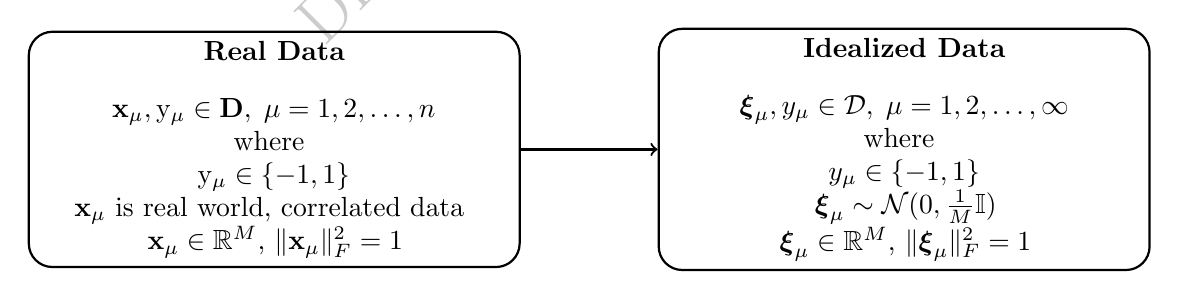
\begin{tikzpicture}[
     thick, % Line thickness
    rectnode/.style={rectangle, draw=black, thick, minimum width=6cm, minimum height=2.5cm, rounded corners=0.3cm}, % Rectangular node style with rounded corners
    -> % Arrow style
]

% Nodes with manual positioning
\node[rectnode] (realdata) at (0,0) {%
    \begin{minipage}{6cm}
        \centering
        \textbf{Real Data} \\
        \vspace{0.3cm}
        $\mathbf{x_\mu}, \mathrm{y}_\mu \in \mathbf{D},\;\mu=1, 2, \ldots, n$\\
        $\text{where }$ \\
        $\mathrm{y}_\mu \in \{-1, 1\}$ \\
        $\mathbf{x_\mu}\text{ is real world, correlated data }$ \\
        $\mathbf{x_\mu} \in \mathbb{R}^{M}$, $\Vert\mathbf{x_\mu}\Vert^{2}_{F}=1$
    \end{minipage}
};

\node[rectnode] (modeldata) at (8,0) {%
    \begin{minipage}{6cm}
        \centering
        \textbf{Idealized Data} \\
        \vspace{0.3cm}
        $\boldsymbol{\xi}_\mu, y_\mu \in \mathbf{\mathcal{D}},\;\mu=1, 2, \ldots, \infty$ \\
        $\text{where }$ \\
        $y_\mu \in \{-1, 1\}$ \\
        $\boldsymbol{\xi}_{\mu} \sim \mathcal{N}(0, \tfrac{1}{M} \mathbb{I})$ \\
        $\boldsymbol{\xi}_{\mu}\in \mathbb{R}^{M}$, $\Vert\boldsymbol{\xi}_{\mu}\Vert^{2}_{F}=1$
    \end{minipage}
};

% Arrow between the boxes
\draw[->] (realdata) -- (modeldata);

\end{tikzpicture}
}
\caption{Mapping from a fixed set of $n$
  real-world, correlated data instances $[\mathbf{x},\mathrm{y}]\in\mathbf{D}$
  to an uncorrelated, random model of idealized data   $[\boldsymbol{\xi}, y]\in\mathbf{\mathcal{D}}$, drawn from a Gaussian i.i.d. distribution.
}
    \label{fig:data_mapping}
\end{figure}


\paragraph{The Data Model.}

To develop a \SemiEmpirical theory of the \Teacher \GeneralizationError, $\TGE^{T}$, 
instead of training and evaluating a NN model using real data $(\DX)$,
we seek a simple, analytical expression with parameters that can be fit to empirical measurements.
So in addition to using a model for our NN, we must specify a model for the data.
In a real NN, the data $\DX$ is correlated, and, in fact, very strongly correlated;
and this is reflected in the layer weight matrices.
However, to be tractable, our starting theoretical expressions use uncorrelated (i.i.d) data.
Formally, we must replace the correlated data 
with some uncorrelated, random model of the data, i.e., $\XVEC\rightarrow\XI$.
As described in Figure~\ref{fig:data_mapping},
our \DataModel is a standard Gaussian $N(0,1)$ model for the input data
\begin{align}
\DATA\rightarrow\XImu,\;\;\XImu\in N(0,1) ,
\label{eqn:mwm_replace_1}
\end{align}
where $N(0,1)$ denotes a Gaussian distribution with zero mean and unit variance,
\and $\XImu$ is normalized such that $\Vert\XImu\Vert=\tfrac{1}{M}$ for all $N$ data vectors.
\michaeladdressed{@charles: I just added a label there, in case you are keeping track of labels.}

We make this distinction between Actual and \ModelData to emphasize that,
later, we will use our so-called \SemiEmpirical procedure to
account for the real correlations in the actual data phenomenologically
by taking some analytical parameter of the theory and fitting it to the real world observations,
here, on the ESD of the NN weight matrices.


\paragraph{The ST Error Model and the Annealed Potential $\EPSLSTx$.}
We now model \Teacher error $\AVGGE^{T}$ with the
\emph{\AverageSTGeneralizationError} $\AVGSTGE$, which is obtained
\michaeladdressed{Is that quite true; doesn't the former involve an extra average, so they are different; see also the comment above on being pedagogically confusing.}
 by \emph{first} computing the ST error function
 %$\Delta\mathbf{E}_{\mathcal{L}}(\SVEC,\TVEC, \XI)$
$\DETOPSTL$
over the set of \emph{all} possible $N$ input examples $\XI$.  Define the data-dependent ST test error function
--or Energy difference--as 
\begin{align}
\label{eqn:DE_L}
%\Delta\mathbf{E}_{\mathcal{L}}(\SVEC,\TVEC, \XI):=\sum_{\mu=1}^{N}\mathcal{L}[E_{NN}(\SVEC,\XI_{\mu}),E_{NN}(\TVEC,\XI_{\mu})]  .
\DETOPSTL:=\sum_{\mu=1}^{N}\mathcal{L}[E_{NN}(\SVEC,\XI_{\mu}),E_{NN}(\TVEC,\XI_{\mu})]  .
\end{align}
where $\mathcal{L}(\SVEC,\TVEC, \XI)$ is simply the $\ell_2$ loss.  This measures the error
between the \Student and the \Teacher; it is zero when their predictions are identical,
$(\Ys=\Yt)$ when $(\XI=\XImu)$, and is nonzero otherwise.

%%5Let us write the Average St \GeneralizationError, $\AVGSTGE$ (formally) as in \EQN~\ref{eqn:finalEgen} as
%%5\begin{align}
%%5\label{eqn:AVGSTGE0}
%%5\AVGSTGE:= & \left\langle\THRMAVG{\Delta\mathbf{E}_{\mathcal{L}}(\SVEC,\TVEC, \XI)}\right\rangle_{\AVGNDXI} 
%%5\end{align}
%%5where we first average over the model data $\NDXI$  and then take a Thermal
%%5average over the \Student weight vectors $\SVEC$.
%%5
%%5We will reduce $\AVGSTGE$ now using the \AnnealedApproximation (AA).
%%5We define two kinds of data-averaged ST errors; the first is used to
%%5define the data-averaged ST \TrainingError, and the second
%%5defines the data-averaged ST test error.
%%5If take the average over the training examples $\XItrain$, we can write
%%5\begin{align}
%%5\label{eqn:ST_train_error}
%%5\langle\Delta\mathbf{E}_{\mathcal{L}}(\SVEC,\TVEC,\XI)\rangle_{\AVGNDXItrain} := \dfrac{1}{\Ntrain}\sum_{\mu=1}^{\Ntrain}\Delta\mathbf{E}_{\mathcal{L}}(\SVEC,\TVEC,\XI_{\mu})
%%5\end{align}
%%5and use this to define the \emph{Model \TrainingError} $\AVGSTTE$.
%%5We dont consider this here,  but it is important for the classic approach;
%%5for a longer discussion, see Section~\ref{sxn:summary_sst92}.
%%5
We aim to derive a simple expression for the  \AverageSTGeneralizationError, $\AVGSTGE$, and to do this, 
we define the  \EffectivePotential for the data-averaged ST \GeneralizationError $\EPSL(\SVEC,\TVEC)$, as in \EQN~\ref{eqn:epsl}, as:
\begin{align}
\label{eqn:STerror}
%\EPSLSTx = \langle\Delta\mathbf{E}_{\mathcal{L}}(\SVEC,\TVEC,\XI)\rangle_{\AVGNDXI}:=\frac{1}{N}\int d\mu(\NDXI)\Delta\mathbf{E}_{\mathcal{L}}(\SVEC,\TVEC,\XI)  ,
\EPSLSTx = \langle\DETOPSTL\rangle_{\AVGNDXI}:=\frac{1}{N}\int d\mu(\NDXI)\DETOPSTL
\end{align}
The measure $d\mu(\NDXI)$ will end up being a Gaussian measure over $N$ samples
(see Appendix~\ref{sxn:summary_sst92}), and the intent is to evaluate it
in the large-$N$ limit, thereby sampling all possible inputs in the model space, $\XI\in\MDD$.

As in \EQN~\ref{eqn:finalEgen} (Section~\ref{sxn:mathP}), by applying the AA, we can rewrite the \AverageSTGeneralizationError, $\AVGSTGE$:
first, a simple average over all the possible inputs $\XI$; and, 
second, then as a Thermal average over all Students $S$, in the AA, and at high-T 
\begin{align}
\label{eqn:MGE}
\AVGSTGE:=\THRMAVG{\EPSLSTx} .
\end{align}
(Recall that in this regime $\AVGSTGE=\AVGGE^{an,hT}$.)


In the classic \STATMECH approach, the average $\THRMAVG{\cdots}$ is
a \ThermalAverage in the canonical ensemble with $\beta$ fixed,
as explained in Section~\ref{sxn:mathP}.  Here, we will do something similar, as the \Student
average $\THRMAVG{\cdots}$ will be computed from the associated
generating function $\IZG$ for the matrix-generalized case  (i.e., an HCIZ integral defined over all students,
and in the large-$N$ limit).)

\michael{MM TO DO: The content of this par is good, it just probably needs to be moved.}
Recall that above, the empirical estimate for $\AVGEMPGE$ depended on a
specific instantiation of the model for the training data $\DATAtrain$,
i.e  $\AVGSTGE$ is \Quenched to the training data.
For that reason, for the final result, we needed to take a second,
quenched average over all possible data sets.
Here, we do not need to consider this and always work in the \AnnealedApproximation(AA).
This is because we incorporate
the specific effects of the real-world training data $(\NDX)$ after we derive our formal expressions
by fitting the model parameters to empirical data.
The final expression for $\AVGSTGE$, derived below,
will be generalized to $\AVGNNGE$, matrix-generalization of  the classic \STATMECH formula
for the \LinearPerceptron, in the \Annealed and High-T approximations.
(see Appendix~\ref{sxn:summary_sst92}). 


%%\subsubsection{The Effective Potential as a function of the overlap $(\EPSL(R))$}
\paragraph{The Annealed Potential as a function of the overlap $(\EPSL(R))$.}

%%In this subsection, we show that the  data-averaged ST test error function (for the $\mathcal{L}=\ell_2$ loss) is:
%%\begin{align}
%%  \EPSL(R)=1-R,\;\;\mathcal{L}=\ell_2
%%\end{align}
%%
We want an expression for the data average of the ST test error, from \EQN~\ref{eqn:STerror}, generalized from \Perceptron vectors to NN layer weight matrices.
\michael{MM TO DO: reword that sentence, since it is a bit confusing, since we are vectors here, and I moved the matrix stuff below to the next section.}
For the \Perceptron, one obtains different expressions for the ST error function, depending on 
the type of activation function $h(x)$ in \EQN~\ref{eqn:ENN};
The simplest are the Linear and Boolean \Perceptrons, and
for both (and with $\ell_2$ loss),
 $\EPSL(\SVEC,\TVEC)$ is simply a function of the ST overlap $R$~\cite{SST92}.
This gives $\EPSLSTx\rightarrow\EPSL(R)$, where
\begin{align}
  \label{eqn:Rdef}
R=\frac{1}{N}\SVEC^{\top}\TVEC=\frac{1}{N}\sum_{i=1}^{M}s_{i}t_{i},
\end{align}
which is simply the dot product between the $M$-dimensional \Student $\SVEC$ and \Teacher $\TVEC$ weight vectors, and normalized by the number of training instances $N$.
For a \LinearPerceptron~\cite{SST92},% 
\footnote{In the classic approach for the ST model, the theory examined different expressions $\EPSL(R)$.
For example, one can consider the  Boolean \Perceptron~\cite{SST92,Ros62}, with activation function $h(x)=\mbox{sgn}(x)$, 
i.e., the Heaviside step function. Then, the error is
$
\EPSL(R)=1 - \dfrac{1}{\pi}\arccos(R).
$
In both cases, perfect learning occurs when $R=1$~\cite{SST92}.
}
with activation function $h(x)=x$,  the error function is
\begin{align}
\EPSL(R)=1-R  .
\label{eqn:LinearPerceptronError}
\end{align}



\begin{figure}[ht]
\centering

%-------------------------------%
% Left image: 2D Overlap
%-------------------------------%
\begin{minipage}{0.48\linewidth}
\centering
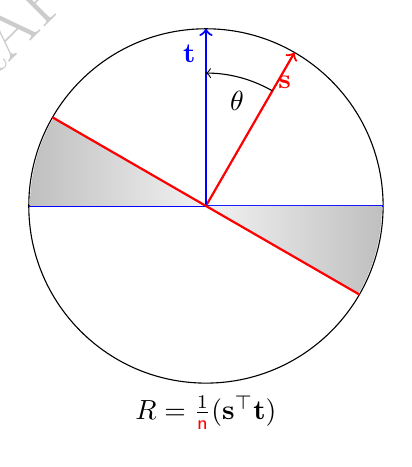
\begin{tikzpicture}[scale=1.5]

    % Circle
    \draw (0, 0) circle (1.5cm);

    % Vectors s (red at 60°) and t (blue at 90°)
    \draw[->,thick,red]  (0,0) -- (60:1.5cm) node[pos=0.7, above right] {\(\mathbf{s}\)};
    \draw[->,thick,blue] (0,0) -- (90:1.5cm) node[pos=0.75, above left] {\(\mathbf{t}\)};

    % Angle theta (between s & t)
    \draw[<-] (0,1.125) arc (90:60:1.125cm) node[pos=0.7, below left] {\(\theta\)};

    % Blue lines (perp. to t = 90°)
    \draw[thick,blue] (0,0) -- (-1.5,0);
    \draw[thick,blue] (0,0) -- ( 1.5,0);

    % Gray shading for overlap region
    \shade[left color=gray!50, right color=gray!10]
      (0,0) -- (-1.49,0) arc (180:150:1.5cm) -- cycle;
    \shade[left color=gray!10, right color=gray!50]
      (0,0) -- (1.49,0) arc (0:-30:1.5cm) -- cycle;

    % Red line(s) perp. to s (60°)
    \draw[thick,red]  (0,0) -- (150:1.5);
    \draw[thick,red]  (0,0) -- (330:1.5); % same as -30°

    % Overlap formula
    \node at (0,-1.75) {\( \AVGR = \frac{1}{\ND} (\mathbf{s}^\top \mathbf{t}) \)};

\end{tikzpicture}
\end{minipage}%
\hfill
%-------------------------------%
% Right image: 3D Overlap (conic sections + wedge)
%-------------------------------%
\begin{minipage}{0.48\linewidth}
\centering
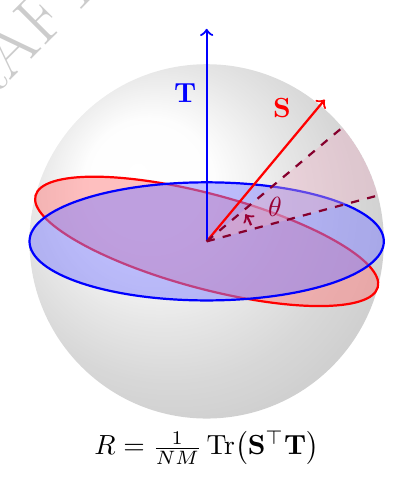
\begin{tikzpicture}[scale=1.5]

    % Light-gray "sphere"
    \shade[ball color=gray!5, opacity=0.3] (0,0) circle (1.5cm);

    % --- Red ellipse for S (unchanged) ---
    \begin{scope}
      \clip (0,0) circle (1.5cm);
      \fill[red!50, opacity=0.5]
        [rotate around={-15:(0,0)}, xscale=1.5, yscale=0.4]
        (0,0) circle (1.0);
    \end{scope}
    \draw[thick, red]
      [rotate around={-15:(0,0)}, xscale=1.5, yscale=0.4]
      (0,0) circle (1.0);

    % --- Blue ellipse for T (CHANGED) ---
    % Make it near-horizontal (rotate=0 or a small angle),
    % and bigger horizontally by increasing xscale significantly.
    \begin{scope}
      \clip (0,0) circle (1.5cm);
      \fill[blue!50, opacity=0.5]
        [rotate around={0:(0,0)},    % CHANGED: no tilt so near x-axis
         xscale=1.5, yscale=0.5]     % CHANGED: bigger horizontally
        (0,0) circle (1.0);
    \end{scope}
    \draw[thick, blue]
      [rotate around={0:(0,0)}, xscale=1.5, yscale=0.5]
      (0,0) circle (1.0);

    % Vectors S (red) & T (blue, vertical & longer)
    \draw[->,thick,red]  (0,0) -- (1.0,1.2)
      node[pos=0.8, above left]  {\(\mathbf{S}\)};
    \draw[->,thick,blue] (0,0) -- (0,1.8)
      node[pos=0.7, left] {\(\mathbf{T}\)};

    % Remove old "theta" arcs

    % -- Fill a wedge (solid angle) in purple --
    \begin{scope}
      \clip (0,0) circle (1.5cm);
      % Let’s pick a narrower wedge from ~15° to ~40°
      \fill[purple!30, opacity=0.4]
        (0,0)
         -- (15:1.5cm)
         arc [start angle=15, end angle=40, radius=1.5cm]
         -- cycle;
    \end{scope}

    % Dashed wedge boundaries
    \draw[thick, dashed, purple!70!black] (0,0) -- (15:1.5cm);
    \draw[thick, dashed, purple!70!black] (0,0) -- (40:1.5cm);

    % Single arc to label theta
    \draw[->, thick, purple!80!black]
      (20:0.4) arc[start angle=20, end angle=35, radius=0.4];
    \node[purple!80!black] at (27:0.65) {\(\theta\)};

    % Overlap formula
    \node at (0,-1.75) {\( \AVGR = \frac{1}{NM} \,\mathrm{Tr}\bigl(\mathbf{S}^\top \mathbf{T}\bigr) \)};

\end{tikzpicture}
\end{minipage}

% Main caption
\caption{Comparison of 2D and 3D representations of the vector and matrix Student--Teacher overlap \(R\).
\textbf{Left:} \(\AVGR = \tfrac{1}{\ND}\mathbf{s}^\top \mathbf{t}\).  Averaged over $\ND$ data samples (implicitly normalized to $1/m$).
\textbf{Right:} \(R = \tfrac{1}{NM}\,\mathrm{Tr}\bigl(\mathbf{S}^\top\mathbf{T}\bigr)\) with conic sections on the sphere (red \(\mathbf{S}\), blue \(\mathbf{T}\)), plus a purple wedge for the angle.  Averaged over matrix dimensions $N$ and $M$ (implicitly normalized over the data $1/\ND$).}
\label{fig:overlaps}
\end{figure}

%\caption{Comparison of 2D and 3D representations of matrix overlap $R$. (a) 2D visualization of vector overlap $R = \cos(\theta) $.
%  (b) 3D visualization of matrix overlap $R = \Trace{\frac{1}{N^2} \SMAT^\top \TMAT $ with solid angle $R$.}



%%\subsubsection{Derivation of the  ST error $(\EPSL(R))$ for the Linear Perceptron}
\paragraph{Derivation of the  ST error $(\EPSL(R))$ for the Linear Perceptron.}
%\nred{WARNING: there may be some mistakes here}
To derive \EQN~\ref{eqn:LinearPerceptronError},
define the data-dependent ST error (\EQN~\ref{eqn:DE_L}) in terms of an $\ell_2$ loss function
%\begin{align}
%\nonumber
%\Delta \mathbf{E}_{\ell_2}(\SVEC,\TVEC,\XI) = & \frac{1}{2} (\Ys - \Yt)^T(\Ys - \Yt) 
%   = 1 - (\YsVEC)^{\top}(\YtVEC) \\ 
%\label{eqn:deriveSTerror}
%   =&  1 - \eta(\XI),
%\end{align}

\begin{align}
\nonumber
\DETOPSTLL= & \frac{1}{2} (\YsVEC - \YtVEC)^{\top} (\YsVEC - \YtVEC) \\
\nonumber
=& \frac{1}{2} \big[(\YsVEC)^{\top} \YsVEC - 2 (\YsVEC)^{\top} \YtVEC + (\YtVEC)^{\top} \YtVEC \big] \\
\nonumber
=& N - (\YsVEC)^{\top} (\YtVEC) \\
\label{eqn:deriveSTerror}
=& N(1 - \ETA(\SVEC,\TVEC)),
\end{align}
where we call $\ETA(\SVEC,\TVEC,\XI):=\tfrac{1}{N}\mathbf{y}_{S}^{\top}\mathbf{y}_{T}$
the \emph{data-dependent \SelfOverlap}.
The expression $\ETA(\SVEC,\TVEC,\XI)$ is analogous to the ST overlap $R$, but before the data has been integrated out.
The \SelfOverlap $\ETA(\SVEC,\TVEC,\XI)$ will appear later in \EQN~\ref{eqn:eta2} (in Section~\ref{sxn:matgen}), 
when formulating the matrix-generalized overlap operator~$\OVERLAP$.

Using the $E_{NN}$ Energy generating or output function (\EQN~\ref{eqn:ENN}), we can replace the label vectors $\YtVEC,\YsVEC$ as
\begin{align}
\YsVEC=\SVEC^{\top}\XI,\;\;
\YtVEC=\TVEC^{\top}\XI  ,
\end{align}
which gives
\begin{align}
  \label{eqn:eta_vec_xi_def}
\ETA(\SVEC,\TVEC,\XI) = \tfrac{1}{N}(\SVEC^{\top}\XI)^{\top} (\TVEC^{\top}\XI) = \tfrac{1}{N}\XI^{\top} (\SVEC^{\top} \TVEC )\XI   .
\end{align}
or, more simply,
\begin{align}
  \label{eqn:eta_vec_avg_def}
\ETA(\SVEC,\TVEC) = \langle\ETA(\SVEC,\TVEC,\XI)\rangle_{\AVGNDXI}=\tfrac{1}{N}(\SVEC^{\top} \TVEC )
\end{align}

We want to evaluate this as an \EffectivePotential $\EPSL(R)$ for the data-averaged ST test error, as in \EQN~\ref{eqn:STerror}.
To do this, we need to compute the average or \ExpectedValue over all possible input data $\XI$,
an $N-$dimensional Gaussian vector (i.e., $d\mu(\XI)=\mathcal{D}\NDXI P(\NDXI)$).
%
%Using $\mathcal{N}$ as the normalization for the average, as yet unspecified, we obtain 
\nred{CHECK THIS: notice we do not include the $\tfrac{1}{N}$ on the R.H.S.}
\begin{align}
 \langle\DETOPSTLL\rangle_{\AVGNDXI}  
   = &\red{\cancel{\frac{1}{\mathcal{N}}}}\int d\mu(\NDXI)(1-\ETA(\XI)) \\ \nonumber
   = &\red{\cancel{\frac{1}{\mathcal{N}}}}\int d\mu(\NDXI)(1-\XI^{\top}\tfrac{1}{N}\SVEC^{\top}\TVEC\XI) \\ \label{eqn:XI_ST} 
   = &\red{\cancel{\frac{1}{\mathcal{N}}}\int d\mu(\NDXI)-\int d\mu(\NDXI)\XI^{\top}\tfrac{1}{N}\SVEC^{\top}\TVEC\XI) } \\ \nonumber
   = & \red{\cancel{\frac{N}{\mathcal{N}}}}1 - \int d\mu(\NDXI)\XI^{\top}\red{\tfrac{1}{N}}\SVEC^{\top}\TVEC\XI \\ \nonumber
   = & \red{\cancel{\frac{N}{\mathcal{N}}}}1 - \int d\mu(\NDXI)\red{\cancel{N}}\XI^{\top} R\XI \\ \nonumber
   = & \red{\cancel{\frac{N}{\mathcal{N}}}}1 - R\int d\mu(\NDXI)\XI^{\top}\XI,
\end{align}
where the fifth line holds because the elements of $\XI$ are i.i.d.\red{???}
Since $d\mu(\NDXI)$ is a measure over a (multi-variate) Gaussian distribution,
if we normalize the data vectors \red{ $\XI$ to $\frac{1}{\sqrt{M}}$ (See Section~\ref{app:st-gen-err-annealed-ham}),  then
\cancel{$\mathcal{N}=N$} the second term on the R.H.S. is unity?} and we recover (i.e., \red{\EQN~\ref{eqn:epsl}})
\begin{align}
\label{eqn:e0}
\EPSL(R)=\langle\DETOPSTLL\rangle_{\AVGNDXI} =  1 - R .
\end{align}
%%%
%%% CHM: what is this ?
%%\begin{align}
%%\frac{1}{N}\langle\Delta \mathbf{E}_{\ell_2}(\SVEC,\TVEC,\XI)\rangle_{\XI}  
%%= &\frac{1}{\mathcal{N}}\int d\mu(\XI)(1-\ETA(\XI)) \\ \nonumber
%%= &\frac{1}{\mathcal{N}}\int d\mu(\XI)(1-\XI^T\SVEC\TVEC^{\top}\XI) 
%%\end{align}
%%where $\mathcal{N}$ is the normalization for the average, as yet unspecified. Expanding, this gives
%%\begin{align}
%%\label{eqn:XI_ST}
%%\frac{1}{N}\langle\Delta \mathbf{E}_{\ell_2}(\SVEC,\TVEC,\XI)\rangle_{\XI} 
%%= & \frac{N}{\mathcal{N}} - \frac{1}{\mathcal{N}}\int d\mu(\XI)\XI^T\SVEC\TVEC^{\top}\XI \\ \nonumber
%%= & \frac{N}{\mathcal{N}} - \frac{1}{\mathcal{N}}\int d\mu(\XI)N\XI^T R\XI \\ \nonumber
%%= & \frac{N}{\mathcal{N}} - R\frac{N}{\mathcal{N}}\int d\mu(\XI)\XI^T\XI,
%%\end{align}
%%where the third line holds because the elements of $\XI$ are i.i.d.
%%Since $d\mu(\XI)$ is a measure over a Gaussian distribution, if we normalize the data vectors $\XI$ to $\frac{1}{\sqrt{N}}$, 
%%then $\mathcal{N}=N$, and we recover 
%%\begin{align}
%%\label{eqn:e0}
%%\EPSL(R)=\frac{1}{N}\langle\Delta \mathbf{E}_{\ell_2}(\SVEC,\TVEC,\XI)\rangle_{\AVGNDXI} =  1 - R .
%%\end{align}

\michaeladdressed{We have several types of subscripts on the BraKet average: $\NDXI$, $\XI$, and $\NDXIn$.  Im not sure if there are typos, or if things are overloaded. The difference isnt clear to me yet.}

In traditional \STATMECH (e.g., \cite{SST92}), one is interested in how the \emph{\TotalModelGeneralizationError} $\TGE(R)$ depends on $R$.
With these simple error functions, \EQN~\ref{eqn:MGE} reduces to a function over $R$,
and the \AverageSTGeneralizationError $\STGE(R)$ is then obtained by averaging over the Students 
\begin{align}
\label{eqn:AVGSTGE_R}
\AVGSTGE(R)=\THRMAVG{\EPSL(R)}=
\THRMAVG{1-\langle\ETA(\SVEC,\TVEC,\XI)\rangle_{\AVGNDXI}}=
\THRMAVG{1-\ETA(\SVEC,\TVEC)}=
\THRMAVG{1-\tfrac{1}{N}\SVEC^{\top}\TVEC}=
\THRMAVG{(1-R)}  ,
\end{align}
where $\THRMAVG{\cdots}$ is a \ThermalAverage over the \Student weight vector $\SVEC$.

Note that the \ModelQuality for the ST \Perceptron, $\Q^{ST}$
is just the \AverageGeneralizationAccuracy, so we can write
\begin{align}
\label{eqn:QST_final}
\Q^{ST} := 1 - \AVGSTGE(R) 
       = \THRMAVG{1 - \EPSL(R)} 
       = \THRMAVG{\langle\ETA(\SVEC, \TVEC, \XI)\rangle_{\AVGNDXI}} 
       = \THRMAVG{\ETA(\SVEC, \TVEC)} 
       = \THRMAVG{\tfrac{1}{N}\SVEC^{\top}\TVEC} 
       = \THRMAVG{R}.
\end{align}
\EQN~\ref{eqn:QST_final} is the starting point for deriving a \SEMIEMP theory for the \WW quality metrics (\ALPHA,\ALPHAHAT);
see Section~\ref{sxn:matgen_mlp3}.
To generalize this expression, we will start with the \SelfOverlap $\ETA(\SMAT,\TMAT,\XI)$ for a
\MultiLayerPerceptron (MLP3) in Section~\ref{sxn:matgen}.

Before doing this, however, we note that 
we can obtain this expression for $\STGE$ by defining the
\AnnealedHamiltonian $\HANHT(R)$, at high-Temperature, as in Section~\ref{sxn:mathP}, \EQN~\ref{eqn:Gan_highT_final}.
Indeed, it is really $\HANHT(R)=\EPSL(R)$ that we must generalize to the matrix case, which we do (using a technique
similar to a Replica calculation, but still in the AA).
For more details, see Appendix~\ref{sxn:summary_sst92}.
(In particular, doing this allows us to define the normalization needed later for the \TRACELOG condition).
\michaeladdressed{MM TO DO: still to work on this par.}


\begin{table}[t]
  \raggedright
\hspace*{-1.5cm}% Adjust this value as needed
\renewcommand{\arraystretch}{1.25} % Increase line spacing in table
\begin{tabular}{|c|c|c|c|}
  \hline
  Quantity & Traditional \SMOG & \makecell{\LinearPerceptron \\ in Traditional \SMOG} & \makecell{Matrix Generalization \\ for \SETOL} \\ \hline

  Total (Idealized) Data Error 
    & $\DETOPXI$ (\ref{eqn:detox})
    & $\DETOPSTL$ (\ref{eqn:deriveSTerror}) 
    & $\DETOPNN$ (\ref{eqn:DE2}) \\ \hline

   Annealed Hamiltonian
    & $\HANHT=\EPSLw$ (\ref{eqn:epsl}) 
    & $\GANHTR=\EPSLSTx=1-\AVGR$ (\ref{eqn:epslR}) 
  & $\GANMATHT = N(\IM-\OVERLAP)$ (\ref{eqn:GANHTmatR}) \\

  (Data-Averaged Error) 
    & (AA, at high-T) 
    & (and at \LargeN) 
    & (only for a layer)  \\ \hline

    \SelfOverlap 
    & $\ETAw = 1-\EPSLw$~(\ref{eqn:def_eta})

    & $\ETA(\SVEC,\TVEC)=\SVEC^{\top}\TVEC$ (\ref{eqn:eta_vec_avg_def})
    & $\ETA(\SMAT,\TMAT)=\tfrac{1}{N}\SMAT^{\top}\TMAT$ (\ref{eqn:eta_mat_avg_def})  \\ \hline
    \hline

  \ModelQuality 
    & $\Q:=1-\AVGGE$ 
    & $\Q^{ST}:=1-\AVGGE^{ST}$ (\ref{eqn:model_qualities})
   & $\Q^{NN}:=1-\AVGGE^{NN}$  (\ref{eqn:model_qualities})\\ 

  in terms of \LayerQuality
    & 
    & 
   & $\Q^{NN}:=\prod_{L} \Q^{NN}_{L}$ \\ \hline
\end{tabular}
\caption{Summary of key quantities compared across traditional \SMOG models,  the \Student-\Teacher (ST) \LinearPerceptron--in the \AnnealedApproximation
(AA) and at high-Temperature (high-T) and at \LargeN in $\ND$, and the matrix-generalized forms as the starting point to frame \SETOL.
The total ST Error of Energy, $\DELBF$, represents the difference (squared) between the model and its labels for the ST model between
the \Student and \Teacher predictions.
The \AnnealedHamiltonian is the Energy function for this Error after it is averaged over the model for the training data
(an $\ND$-dimensional i.i.d. idealized Gaussian dataset,  $\NDXIn$).
In the AA, the \AnnealedHamiltonian is equal to the \EffectivePotential.  For the ST model,  this is one minus the average overlap, $\HANHT(R)=(1-\AVGR)$;
for the \SETOL, this is  the ($M$-dimensional) identity minus the overlap operator/matrix, $\HANHT(\OVERLAP)=N(\IM-\OVERLAP)$. 
The \SelfOverlap $\eta(\cdots)$ is used to describe the Accuracy (as opposed to the Error) for both the ST model and
its matrix-generalized form.
%Notice that $\eta(\XI)$, as defined,  has not yet been averaged over the model data $\XI^{N}$.
Finally, the different forms of the \Quality are defined.  Generally speaking, the \Quality $\Q$ is an approximation to some measure
of $1$ minus the \AverageGeneralizationError, $\Q:=1-\AVGGE$ (in the AA, at high-T, at \LargeN, and with whatever else
approximations are applied).
For the ST model, having just 1 layer, the \ModelQuality and the \LayerQuality are the same, and denoted $\Q^{ST}$.
For \SETOL, the \ModelQuality $\Q^{NN}$ is a product of individual \LayerQualities $\Q^{NN}_{L}$.
(Note that the  final \SETOL \LayerQuality $\Q$ is defined in terms of the \LayerQualitySquared $\QT$,
and the starting point for this is expressed with the \LayerQualitySquared Hamiltonian $\HBARE=\OLAPTOLAP$.
}
\label{table:quantities_general_vect_matrix}
\end{table}



\newpage
\section{\SemiEmpirical Theory of the \HTSR Phenomenology}
\label{sxn:matgen}

In this section, we present the main technical elements of our \SemiEmpirical Theory of Deep Learning (\SETOL).
Our goal is to explain and, where possible, derive the \HTSR PL metrics \ALPHA $(\alpha)$ and \ALPHAHAT $\hat{\alpha}$
from first principles, and, in doing so, also present the \TRACELOG condition and
newly proposed \WW\DETX metric.
To do this, we introduce a Matrix Generalization of the Student-Teacher model for a Linear \Perceptron
(See Section~\ref{sxn:SMOG_main-st_av}), 
adapted here for a (3-layer) \MultiLayerPerceptron  (MLP3).
We seek a theory for the \LayerQuality $\Q=\Q^{NN}_{L}$ of a NN, where
this \LayerQuality now corresponds to the (approximate) contribution each layer makes to the total
generalization accuracy, or total \Quality $\Q^{NN}$.
For technical reasons, we actually seek a formal expression(s) for the \LayerQualitySquared,
$\QT\approx\Q^{2}$.
We say that the \SETOL is \SemiEmpirical because the final result $\QT$ is expressed directly in terms
of the empirically observable spectral properties of the Teacher layer weight matrix $\TMAT=\WMAT$.


%\red{REMOVED OUTLINE REPACE WITH SECTION 5.1: need to rework the paragraph above and below, merge}
%\paragraph{Outline}
%\begin{itemize}
%\item In Section~\ref{sxn:matgen_basic_elements}, we provide an overview of basic elements of our approach.
%
%\item In Section~\ref{sxn:matgen_mlp3}, we describe the matrix generalization of the ST  model of the \LinearPerceptron.
%
%\item In Section~\ref{sxn:matgen_quality_hciz}, we describe how to generalize the (Thermal) average over the Students to an integral over random \Student matrices, called an HCIZ integral.
%
%\item In Section~\ref{sxn:matgen_evaluation_hciz}, we describe how to evaluate the HCIZ integral in the large-$N$ limit.
%
%\item In Section~\ref{sxn:r_transforms}, we explain how to select an \RTransform and evaluate the \michael{such-and-such-not-sure-if-we-should-call-it-norm-gf} under different modeling assumptions.
%\end{itemize}

%%\subsection{Basic Elements of the \SemiEmpirical Theory}
%\label{sxn:matgen_basic_elements_concise}

\begin{enumerate}[label=5.\arabic*]
\item
\textbf{Matrix Generalization of the ST Model.}
Section~\ref{sxn:matgen_mlp3} generalizes
classical \STATMECH vector-based ST model of Section~\ref{sxn:SMOG_main-student_teacher}
to obtain a \LayerQuality for a single layer in a NN.
It starts by first formulating the learning problem for
the NN generalization accuracy or quality, $\Q^{NN}$,
of a 3-layer MLP (MLP3).
We then replace vectors with $N \times M$ matrices $\SVEC,\TVEC\rightarrow\SMAT,\TMAT$,
and obtain and expression for the NN \SelfOverlap $\ETA(\SMAT,\TMAT,\XI)$,which then gives a matrix-generalized overlap operator
$\OVERLAP:=\langle\ETA(\SMAT,\TMAT,\XI)\rangle_{\AVGNDXI}=\tfrac{1}{N}\SMAT^{\top}\TMAT$.
This can be related to a single-layer matrix-generalization of the ST \AnnealedHamiltonian, 
presented in Appendix~\ref{sxn:summary_sst92},
$\HANHT:=\red{N}(M-\OVERLAP$),
where, importantly, the scalar overlap $R$ is now a matrix $\OVERLAP$ of $M\times M$ adjustable parameters.
\red{And, importantly, being empirical quantities, the matrices are implicitly normalized to $1/\ND$.}

\item
\textbf{The \LayerQualitySquared $\QT$.}
Section~\ref{sxn:matgen_quality_hciz} presents the expression for NN \LayerQualitySquared $\QT$.
Following the ST analogy, we define a \ThermalAverage over possible \Student weight matrices $\SMAT$
for the matrix overlap, giving $\Q^{NN}_{L}:=\THRMAVGIZ{\HANHT} =\THRMAVGIZ{\OVERLAP}$.
For technical reasons, however, we actually seek the (approximate)  \LayerQualitySquared, $\QT\approx (\Q^{NN}_{L})^2$,
defined as $\QT:=\THRMAVGIZ{\OLAPTOLAP}$.
To evaluate $\QT$, rather than sampling all random \Student matrices $\SMAT$ directly,
we switch measures to the (Outer) \Student Correlation matrices\footnote{
We adopt the convention ``Inner'' for smaller, $M\times M$ full rank \Student correlation matrices, and ``Outer'' for larger, $N\times N$ rank-deficient \Student Correlation matrices.
Note that both are scaled as $1 / N$, meaning that their nonzero eigenvalues are the same.
} 
$\AMATN = \tfrac{1}{N}\SMAT\SMAT^{\top}$ along with their Inner counterparts
$\AMATM = \tfrac{1}{N}\SMAT^{\top}\SMAT$.
Importantly, we argue that the measures $d\mu(\AMATM)\leftrightarrow d\mu(\AMATN)$,
can be interchanged for our purposes, making them effectively equivalent.
This reparameterization leads us to an integral of the HCIZ type (as in \EQN~\ref{eqn:hciz_prelim})
which, as shown by Tanaka \cite{Tanaka2007, Tanaka2008}, can be described in terms of its R-transform.

Then, we introduce the \EffectiveCorrelationSpace (\ECS), and two key approximations,
the \TRACELOG Condition and the \IndependentFluctuationApproximation (\IFA).
The \TRACELOG condition states that the determinant of the (effective) \Student correlation matrix is unity, $\Det{\AECS}=1$.
Critically, this condition can be tested empirically by assuming the (effective) \Teacher correlation matrix
also follows the \TRACELOG condition, $\Det{\XECS}=1$, and this is a key result of this work.
Finally, we impose the \IFA (described below) because it is necessary for the final result.

\item
\textbf{The \LargeN limit in $N$}
Section~\ref{sxn:matgen_evaluation_hciz} presents the core result,
(as in \EQN~\ref{eqn:QT_result}),
closed-form or semi-analytic expression(s) for the \LayerQualitySquared $\QT$
formed in the "wide" \largeN limit in $N$.
Restricted to the \ECS, and under the \TRACELOG condition and the \IFA, our
HCIZ integral for $\QT$ becomes tractable at large-$N$, giving an expression that can be parameterized
in terms of $\MECS$ eigenvalues $\LambdaECS$ of the \Teacher correlation matrix 
restricted to the \ECS $\XECS$.
In doing this, the $\MECS$ \Teacher eigenvalues are treated as experimental observables, and 
become the effective \SemiEmpirical parameters (i.e., $\alpha$, $\LambdaMax$) of our \SETOL.

\item
\textbf{Modeling the \HeavyTailed \RTransform}
Section~\ref{sxn:r_transforms} presents several models of different \RTransforms.
Evaluating $\QT$ requires evaluating selecting an \RTransform $R(z)$ for the Teacher Empirical Spectral Density (ESD),
and also ensure that it is analytic and single-valued on the domain of interest-- the \ECS and/or tail of the ESD.
We examine four possible models for $R(z)$: \emph{(i)} the \emph{Bulk$+$Spikes} (BS),
\emph{(ii)} the \emph{Free Cauchy} (FC) model, 
\emph{(iii)} the \emph{\InverseMP} (IMP) model, 
and \emph{(iv)} the  \LevyWigner (LW) model.
First, as a trivial case, the tail of ESD can be treated as a collection of spikes,
and the ESD is simply a sum of Dirac delta functions; in this case,
$\QT$ becomes a ``Tail Norm'', the Frobenius Norm of the PL tail.
When the layer is \Ideal, i.e., $\alpha\sim 2$ and $\Det{\XECS}\sim 1$,
one can use  \emph{Free Cauchy} (FC) model.  and the resulting \LayerQuality $\Q$
is approximately the Spectral Norm $\LambdaMax$.
Since $\LambdaMax$ increases with decreasing $\alpha$, the FC model yields the \HTSR \ALPHA metric.
One can also use  \emph{\InverseMP} (IMP) model. 
As required, the IMP \RTransform contains a \emph{branch cut} in the complex plane
which aligns with the start of the \ECS \PowerLaw tail.
Finally, Using the \LevyWigner (LW) model, one can model cases where
$\alpha\le 2$ and derive the \HTSR \ALPHAHAT metric.
\end{enumerate}

\vspace*{1em}

These core elements form a bridge between well-established empirical properties of large-scale NNs 
and a tractable ST-based theory. In the subsequent sections, we formalize the key steps: 
\emph{(i)} setting up the matrix-based ST problem, \emph{(ii)} defining our HCIZ integrals 
over restricted correlation matrices (\ECS), and \emph{(iii)} analyzing the resulting 
\emph{Layer Quality} (or \emph{Quality-Squared}) expressions in the large-$N$ limit.

%\subsection{Basic Elements of the \SemiEmpirical Theory}
%\label{sxn:matgen_basic_elements_concise}

\begin{enumerate}[label=5.\arabic*]
\item
\textbf{Matrix Generalization of the ST Model.}
Section~\ref{sxn:matgen_mlp3} generalizes
classical \STATMECH vector-based ST model of Section~\ref{sxn:SMOG_main-student_teacher}
to obtain a \LayerQuality for a single layer in a NN.
It starts by first formulating the learning problem for
the  NN generalization accuracy or quality, $\Q^{NN}$,
of a  3-layer MLP (MLP3).
We then replace vectors with $N \times M$ matrices $\SVEC,\TVEC\rightarrow\SMAT,\TMAT$,
and obtain and expression for the NN \SelfOverlap $\ETA(\SMAT,\TMAT,\XI)$,
which then gives a matrix-generalized overlap operator
$\OVERLAP:=\langle\ETA(\SMAT,\TMAT,\XI)\rangle_{\AVGNDXI}=\tfrac{1}{N}\SMAT^{\top}\TMAT$.
This can be related to a single-layer matrix-generalization of the ST \AnnealedHamiltonian, 
presented in Appendix~\ref{sxn:summary_sst92}, $\HANHT:=M-\OVERLAP$,
where, importantly, the scalar overlap $R$ is now a matrix $\OVERLAP$ of $M$ adjustable parameters.

\item
\textbf{The \LayerQualitySquared $\QT$}
Section~\ref{sxn:matgen_quality_hciz} presents the expression for NN \LayerQualitySquared $\QT$.
Following the ST analogy, we define a \ThermalAverage over possible \Student weight matrices $\SMAT$
for the matrix overlap, giving $\Q^{NN}_{L}:=\THRMAVGIZ{\HANHT} =\THRMAVGIZ{\OVERLAP}$,
For technical reasons, however, we actually seek the (approximate)  \LayerQualitySquared, $\QT\approx\Q^{2}$,
defined as $\QT:=\THRMAVGIZ{\OLAPTOLAP}$.
To evaluate $\QT$, rather than sampling all random \Student matrices $\SMAT$ directly,
we switch measures to the \Student correlation matrices 
$\AMAT_{2} = \tfrac{1}{N}\SMAT\SMAT^{\top}$.
Importantly, we argue that the measures $d\mu(\AMAT_{1})\leftrightarrow d\mu(\AMAT_{2})$,
can be interchanged for our purposes, making them effectively equivalent.
This reparametrization leads us to an integral of the HCIZ type (as in \EQN~\ref{eqn:hciz_prelim})
which, as shown by Tanaka \cite{Tanaka2007, Tanaka2008}.

Then, we introduce the \EffectiveCorrelationSpace (\ECS), and two key approxmations,
the \TRACELOG Condition and the \IndependentFluctuationApproximation (\IFA).
The \TRACELOG condition states that the determinant of the (effective) \Student correlation matrix is unity, $\Det{\AECS}=1$.
Critcially, this condition can be tested empirically by assuming the (effective) \Teacher correlation matrix
also follows the \TRACELOG condition, $\Det{\XECS}=1$, and this is a key result of this work.
Finally, we impose the \IFA (described below) because it is necessary for the final result.

\item
\textbf{The Large-$N$ limit}
Section~\ref{sxn:matgen_evaluation_hciz} presents the core result,
(as in \EQN~\ref{eqn:QT_result}),
a closed-form or semi-analytic expressions for the \LayerQualitySquared $\QT$
formed in the large-$N$ limit.
Restricted to the \ECS, and under  the \TRACELOG condition and the \IFA, our
HCIZ integral for $\QT$ becomes tractable at large-$N$, givin an expression that can be parameterized
in terms of $\MECS$ eigenvalues $\LambdaECS$ of the \Teacher correlation matrix 
restricted to the \ECS $\XECS$.
In doing this, the $\MECS$ \Teacher eigenvalues are treated as experimental observables, and 
become the effective \SemiEmpirical parameters (i.e, $\alpha$, $\lambda_{max}$) of our \SETOL.

\item
\textbf{Modeling the \HeavyTailed \RTransform}
Section~\ref{sxn:r_transforms} presents several  models of different \RTransforms.
Evaluating $\QT$ requires evaluating selecting an \RTransform $R(z)$ for the Teacher ESD,
and also ensure that it is analytic and single-valued on the domain of interest-- the \ECS and/or tail of the ESD.
We examine four possible models for $R(z)$: \emph{(i)} the \emph{Bulk$+$Spikes} (BS),
\emph{(ii)} the \emph{Free Cauchy} (FC) model, 
\emph{(iii)} the \emph{Inverse Wishart} (IW) model, 
and \emph{(iv)} the  \LevyWigner (LW) model.
First, as a trivial case, the tail of ESD can be treated as a collection of spikes,
and the ESD is simply a sum of Dirac delta functions; in this case,
$\QT$ becomes a ``Tail Norm'', the Frobenius Norm of the PL tail.
When the layer is \Ideal, i.e., $\alpha\sim 2$ and $\Det{\XECS}\sim 1$,
one can use  \emph{Free Cauchy} (FC) model.  and the resulting \LayerQuality $\Q$
is approximately the Spectral Norm $\lambda_{max}$.
Since $\lambda_{max}$ increases with decreasing $\alpha$, the FC model yields the \HTSR \ALPHA metric.
One can also use  \emph{Inverse Wishart} (IW) model. 
As required, the IW \RTransform contains a \emph{branch cut} in the complex plane
which aligns with the start of the \ECS \PowerLaw tail.
Finally, Using the \LevyWigner (LW) model, one can model cases where
$\alpha\le 2$ and derive the \HTSR \ALPHAHAT metric.
\end{enumerate}

\vspace*{1em}

These core elements form a bridge between well-established empirical properties of large-scale NNs 
and a tractable ST-based theory. In the subsequent sections, we formalize the key steps: 
\emph{(i)} setting up the matrix-based ST problem, \emph{(ii)} defining our HCIZ integrals 
over restricted correlation matrices (\ECS), and \emph{(iii)} analyzing the resulting 
\emph{Layer Quality} (or \emph{Quality-Squared}) expressions in the large-$N$ limit.

\subsection{\MultiLayer Setup: MLP3}
\label{sxn:matgen_mlp3}

In this section, we describe the matrix generalization of the ST  model of the \LinearPerceptron; and, 
in particular, a matrix-generalized version of the key quantities we derived in Section~\ref{sxn:SMOG_main-st_av}.

\paragraph{A simple model.}

Consider a simple NN with three layers (two hidden and an output), i.e., a three-layer \MultiLayerPerceptron, denoted as the \emph{MLP3} model.
(This is a \emph{very} simple model of a modern NN with hundreds of layers and complex internal structure.)

Ignoring the bias terms, \emph{Without Loss of Generality}, (WLOG), the NN outputs
 $E_{1\mu},E_{2\mu},E_{3\mu}$ for each layer, as defined in \EQN~\ref{eqn:dnn_energy}, are given by:
\begin{align}
\nonumber
  E_{1\mu} &:= \frac{1}{\sqrt{N_1}} h (\mathbf{W}_1^\top \boldsymbol{\xi}_{\mu}) , \\
\nonumber
  E_{2\mu} &:= \frac{1}{\sqrt{N_2}} h (\mathbf{W}_2^\top \mathbf{Z}_{1\mu})     , \\
\label{eqn:nflow}
             y_{\mu} := E_{3\mu} &= \frac{1}{\sqrt{N_3}} h (\mathbf{W}_{3}^\top \mathbf{Z}_{2\mu})     ,
\end{align}
where $h$ is a general function or functional, denoting either a non-linear activation or a more complex layer structure, such as a CNN or an RNN.
We can consider $h(\cdot)$ to be an (unspecified) activation function.

Let us specify the ST error, or Energy difference, specifically in terms of the L2 or RMSE loss:
\begin{equation}
\label{eqn:DE}
\DETOPNN = \frac{1}{2}\sum_{\mu=1}^{\ND} (\Ys - \Yt)^2.
\end{equation}

We now start to develop the self-overlap \(\eta\) using \(\mathbf{S} - \mathbf{T}\):

\subsubsection{Data-Dependent Multi-Layer ST Self-Overlap $(\ETA(\SMAT,\TMAT))$}

It is convenient to rewrite $\Delta \mathbf{\hat{E}}$ in \EQN~\ref{eqn:DE} as:
\begin{align}
\label{eqn:DE2}
\DETOPNN
   := \frac{1}{2} \Trace{ (\Ys - \Yt)^\top (\Ys - \Yt) }
   = N - \Trace{ (\YsVEC)^{\top} \, \YtVEC  }
   = N(1 - \ETAMLPXI)
\end{align}
where the \SelfOverlap $\ETAMLPXI$
is of the same form as the (vector) \LinearPerceptron (in \EQN~\ref{eqn:deriveSTerror}).
Note that $\ETAMLPXI$ depends on the (model) data $\boldsymbol{\xi}$
because we have not evaluated the expected value $\langle \cdots \rangle_{\boldsymbol{\xi}}$ yet.

Using the general expression from \EQN~\ref{eqn:nflow} for the action of the NN on the input data $\boldsymbol{\xi}$,
we can write the formal expression of the ST error for the simple MLP3 model as:
\begin{align}
\label{eqn:overlap1}
\ETAMLPAVG  \\ \nonumber
& =\langle\ETA(\SMAT_1,\SMAT_2,\SMAT_3,\TMAT_1,\TMAT_2,\TMAT_3,\boldsymbol{\xi})\rangle_{\AVGNDXI}  \\ \nonumber
& :=  \Trace{
    \frac{1}{\sqrt{N_3}} h\left(\mathbf{S}_3^{\top} 
    \frac{1}{\sqrt{N_2}} h\left(\mathbf{S}_2^{\top} 
    \frac{1}{\sqrt{N_1}} h\left(\mathbf{S}_1^{\top} \boldsymbol{\xi} \right)\right)\right)^{\top} 
    \times
    \frac{1}{\sqrt{N_3}} h\left(\mathbf{T}_3^{\top} 
    \frac{1}{\sqrt{N_2}} h\left(\mathbf{T}_2^{\top} 
    \frac{1}{\sqrt{N_1}} h\left(\mathbf{T}_1^{\top} \boldsymbol{\xi} \right)\right)\right)
  }.
\end{align}

So far, we have not used any particular assumption on the form of the NN or the data, 
\michael{But this is the model Gaussian data, not the real data}
\charles{Yeah, I guess thats in the notation, but we have not integrated out the data yet.  We can rephrase this}
other than that the layer structure used to write the explicit expression for the form eventually xneeded,
$\ETA(\SMAT,\TMAT)$, a single layer \SelfOverlap.
As a next step, we show which assumptions are needed in order to reformulate the setup as
an effectively a single layer linear model for a NN.

\michael{The following change to single layer holds for L2 and non-L2, correct?  If so, why mention L2 in \EQN~\ref{eqn:DE} and \EQN~\ref{eqn:DE2}, and then go back to more general in \EQN~\ref{eqn:overlap1}.}
\charles{um no I think the square is necessary }

\subsubsection{A Single Layer Matrix Model}

Following others in the literature~\cite{SMG2013_TR}, and for simplicity, one can restrict to the simplifying case that the function $h(x)$ is the identity function.
To evaluate \EQN~\ref{eqn:overlap1}, there are three possibilities.
First, we can multiply all the matrices together, and treat a multi-layer NN effectively as a single layer.
Under this assumption, \EQN \ref{eqn:overlap1} simplifies to
%
\begin{align}
\label{eqn:overlap2}
  \ETAMLPAVG &= \tfrac{1}{N_3 \, N_2 \, N_1} 
  \Trace{ \boldsymbol{\xi}^\top 
    \mathbf{S}_1 \mathbf{S}_2 \mathbf{S}_3 
    \mathbf{T}_3^{\top} \mathbf{T}_2^{\top} \mathbf{T}_1^{\top} 
    \boldsymbol{\xi} }.
\end{align}
While this is possible, it would not lead to layer-by-layer insights (as \HTSR-based approaches do).
%
Second, we could attempt to expand \EQN~\ref{eqn:overlap2} into inter- and intra-layer terms, 
which we could readily do if the $S$ and $T$ matrices were square and the same shape, and then apply Wicks theorem:
\begin{align}
\ETAMLP\approx\prod_{l=1}^{L}\tfrac{1}{N_l}\ETAMATAVG=\prod_{l=1}^{L}\tfrac{1}{N_l}\Trace{ \XI^{\top} \mathbf{S}^{\top}_{l} \mathbf{T}_{l} \XI) } +\text{intra-layer cross terms}.
\end{align}
However, these matrices are not square, and we don't know how to express the intra-layer cross terms.
%
Finally, we can simply assume that the individual layers are statistically independent, in which case we can treat each layer independently.
By ignoring the intra-layer cross-terms, let us write the single-layer self-overlap $\ETAMAT$ as:
\begin{align}
  \label{eqn:eta}
  \ETAMAT =
        \ETAMATAVG\rightarrow \tfrac{1}{N} \Trace{ \XI^{\top} \mathbf{S}^{\top}_{l} \mathbf{T}_{l} \XI }  .
\end{align}
This third approach is the one we will adopt.
Moving forward, we will drop the layer subscript, $l$, and we will consider a \SETOL as a single-layer theory.


\subsubsection{The Matrix-Generalized ST Overlap $(\ETA(\SMAT,\TMAT)$)}

We can now relate the \SelfOverlap for the NN layer $\ETA(\XI)_{l}$ in \EQN~\ref{eqn:eta}
as a matrix-generalized form of the ST \EffectivePotential $\EPSL(R)=1-R$.
\michaeladdressed{We are calling it \EffectivePotential there; not sure if we are going to use that term or the other, consistently throughout.}
Since we can interpret the Trace as an expected value over the model data $\NDXI$, this gives the desired
\begin{align}
  \label{eqn:eta_mat_avg_def}
  \ETA(\SMAT,\TMAT)
  :=\tfrac{1}{N} \Trace{\mathbf{S}^{\top}\mathbf{T}} 
\end{align}
This is the matrix generalized form of \EQN~\ref{eqn:QST_final} for the \LayerQuality.


\subsection{Quality Metrics of an Individual Layer as an HCIZ Integral}
\label{sxn:matgen_quality_hciz}

In this subsection, we describe how to generalize the (Thermal) average over the Students $\THRMAVG{\cdots}$ to an 
integral over random \Student matrices, $\THRMAVGIZ{\cdots}$, called an HCIZ integral.

\subsubsection{A Generating Function Approach to Average \QualitySquared of a Layer}
\label{sxn:matgen_quality_hciz_A}

For our matrix generalization, we need to express the \LayerQuality $\Q$ in terms of the data-averaged
\SelfOverlap in \EQN~\ref{eqn:eta_mat_avg_def} for a individual layer.
\begin{itemize}
\item
\textbf{Student-Teacher Overlap  $\mathbf{R}$}
For the vector-based \Perceptron ST model, the data-averaged \SelfOverlap appears in the expression for the
\LayerQuality  in \EQN~\ref{eqn:QST_final}, and is just the average ST vector overlap $R=\SVEC^{\top}\TVEC$. 
We define 
\begin{equation}
\mathbf{R} =  \frac{1}{N}\SMAT^{T} \TMAT  .
\end{equation}
The overlap matrix $\OVERLAP$ describes the average interactions between $N$ interacting $M$-dimensional layer (i.e., feature) vectors.  Also, notice that we have dropped $1/\ND$ term.
For the vector-based ST model, the ST \Quality $\Q^{ST}$ in \EQN~\ref{eqn:QST_final} is expressed as
the \ThermalAverage $\Q^{ST}(\AVGR)=\THRMAVG{\AVGR}$. We seek a similar formal expression for the individual matrx-generalized \LayerQuality $\Q^{NN}_{L}$.
\item
\textbf{Model and Layer Qualities $\Q^{NN}$, $\Q^{NN}_{L}$}
We define the \ModelQuality $\Q^{NN}$ ,
as explained in Subsection~\ref{sxn:htsr-metics}, \EQN~\ref{eqn:ProductNorm},
to be a product of individual NN Layer Qualities $\Q^{NN}_{L}$,
and, as in \EQN~\ref{eqn:model_qualities},
approximates the total NN \AverageGeneralizationAccuracy $(1-\AVGGE^{NN})$:
\begin{equation}
 \Q^{NN}:=\prod_{L}\Q^{NN}_{L}\approx 1-\AVGGE^{NN} 
\end{equation}
The individual $\Q^{NN}_{L}$ expresses the contribution that layer makes
to the approximate total NN \AverageGeneralizationAccuracy.
\item
 \textbf{\LayerQualitySquared $\QT$}
For  technical convenience, however, rather than compute
the NN \LayerQuality $\Q^{NN}_{L}$ directly, we will work with the \emph{\AverageLayerQualitySquared}, 
defined as
\begin{align}
  \label{eqn:QT_1}
  \QT:=\THRMAVGIZ{\OLAPTOLAP}
\end{align}
where  $\THRMAVGIZ{\cdots}$ is now a \ThermalAverage over Student weight matrices $\SMAT$--
an HCIZ integral.

This choice means that final \LayerQuality $\Q$ we use approximates what would be the
matrix-generalized NN \LayerQuality $\Q^{NN}_{L}$ (above) as
\begin{align}
  \label{eqn:QT_2}
  \Q:=\sqrt{\QT}
  =\sqrt{\THRMAVGIZ{\OLAPTOLAP}} \\ \nonumber
  \approx\THRMAVGIZ{\sqrt{\OLAPTOLAP}} \\ \nonumber
  \approx\THRMAVGIZ{\OVERLAP} \\ \nonumber
  = \Q^{NN}_{L}
\end{align}

\item
 \textbf{Overlap Squared}
 The Overlap operator (squared)  $\OLAPSQD$ is defined  in terms of \EQN~\ref{eqn:A2} such
 that we can 
\begin{align}
  \label{eqn:TraceR2withA2}
  \QT :=\OLAPSQD
  =\frac{1}{N^{2}}\Trace{\TMAT^{\top}\SMAT\SMAT^{\top}\TMAT}
  =\frac{1}{N}\Trace{\TMAT^{\top}\AMATN\TMAT}  .
\end{align}
This choice, (as opposed to $\Trace{\OVERLAP\OVERLAP^{\top}}$, which would correspond with \EQN~\ref{eqn:A1},) places $\QT$ in the form of the HCIZ integral, as in \EQN~\ref{eqn:hciz_prelim}.
See Appendix~\ref{sxn:tanaka} for a detailed discussion of why we define $\QT$ using the \emph{Outer} Student Correlation matrix $\AMATN$ (defined in Section~\ref{sxn:setol}, and  \EQN~\ref{eqn:A2} below).
\item
 \textbf{\GeneratingFunction}
For the vector-based ST model, we could compute $\Q^{ST}$ using a generating function, $\STG$.
For our matrix generalization, we compute $\Q$ from a \emph{\LayerQualitySquared \GeneratingFunction} $\IZG$, given as
\begin{align}
  \label{eqn:betaIZG_S}
  \IZG:=  \red{\tfrac{1}{N}}\ln \int d\mu(\SMAT) \exp\left[\ND\beta N\OLAPSQD\right] .
\end{align}
We normalize the $\IZG$ because we are going to take the \LargeN limit in $N$, and we need to keep the \LayerQuality finite.  This allows us to implicitly fix the effective load of the layer, $\ND/N$, as $\IZG$ is also in the \ThermodynamicLimit and therefore at \LargeN in $\ND$, although we do not explicitly set $\ND/N$.
See Appendix~\ref{sxn:quality} for the derivation of \EQN~\ref{eqn:betaIZG_S} (and recall the discussion in Section~\ref{sxn:mathP}). 
\end{itemize}

We cannot evaluate \EQN~\ref{eqn:betaIZG_S} directly; but we will be able to evaluate it if we transform it into an HCIZ integral (as in \EQN~\ref{eqn:hciz_prelim}). To do this, however, requires a trick which will allow us to work with different forms of the Student $\AMAT$ (and Teacher $\XMAT$) Correlation matrices.

\paragraph{From weight matrices to Correlation matrices.}
To evaluate $\QT$ in terms of derivatives of \EQN~\ref{eqn:betaIZG_S}, we need to introduce the change of measure:
\begin{align}
  \label{eqn:changeOfMeasure}
  d\mu(\SMAT)\rightarrow d\mu(\AMAT) ,
\end{align}
and then restrict $d\mu(\AMAT)$ to resemble just the generalizing eigencomponents of the \Teacher correlation matrix $\XMAT$.
%
%MM%
%MM%We now introduce the change of measure
%MM%\begin{align}
%MM%  \label{eqn:changeOfMeasure}
%MM%  d\mu(\SMAT)\rightarrow d\mu(\AMAT)
%MM%\end{align}
%MM%So before we evaluate $\QT$, we need to do this change of measure,
%MM%and do so that we restrict $d\mu(\AMAT)$ to resemble the just the
%MM%generalizing eigen-components of the \Teacher correlation matrix $\XMAT$.
%MM%
%\paragraph{Two choices for $\AMAT$}
We have two choices for the \Student \CorrelationMatrix $\AMAT$, call them $\AMATM$
(Inner) and $\AMATN$ (Outer), defined as:
\begin{eqnarray}
  \label{eqn:A1}
 \textrm{(Inner) }\;\AMATM&:=& \frac{1}{N}\SMAT^{\top}\SMAT \quad\mbox{(which is $M \times M$)} \\
  \label{eqn:A2}
 \textrm{(Outer) }\;\AMATN &:=& \frac{1}{N}\SMAT\SMAT^{\top} \quad\mbox{(which is $N \times N$)} .
\end{eqnarray}
Note that $\frac{1}{N}$ is the correct scaling on each of these.
\EQN~\ref{eqn:A1} is consistent with our definition of the layer \CorrelationMatrix, and we use it as the starting point
below to derive the \VolumePreserving \TRACELOG condition (Appendix~\ref{sxn:TraceLogDerivation}).
\EQN~\ref{eqn:A2} is consistent with Tanaka, which requires $\AMAT$ be $N\times N$, but
we still need a \emph{Duality of Measures} to rederive this (Appendix~\ref{sxn:tanaka})~\cite{Tanaka2007, Tanaka2008}.

\paragraph{Duality of measures.}
For either form of $\AMAT$, the measure $d\mu(\AMAT)$ is the same because we will restrict the measures to the~\ECS
space of non-zero eigenvalues $(\lambda_{i}\gg 0)$.
We note that $\AMATM$ and $\AMATN$ have the same eigenvalues $\lambda_{i}$, or ESD,
up to the additional zero eigenvalues $(\lambda_{i}=0)$ in the null space of $\AMATN$.  
Consequently, both forms of $\AMAT$ have 
the same non-zero part
of the ESD $(\rho(\lambda)\gg 0)$, and the same Trace $(\Trace{\AMATM}=\Trace{\AMATN})$.
In the large-N approximation, the ESD of (either form of)
$\AMAT$, $\rho^{\infty}_{\AMAT}(\lambda)$,
becomes continuous (and bounded), but remains zero in the null space.
(Notice that following the physics approach, in the limit, $N$ remains finite but we nevertheless assume a continuous spectrum)
Consequently,
when integrating over the eigenvalues  $\lambda$, one can interchange
$\AMATM$  with $\AMATN$, such that
\begin{align}
 \int d\mu(\AMAT)\;[\cdots]\;\leftrightarrow  \int d\lambda\;[\cdots]\; \rho^{\infty}_{\AMATM}(\lambda) \leftrightarrow  \int d\lambda\;[\cdots]\; \rho^{\infty}_{\AMATN}(\lambda)
\end{align}
This equivalence will be essential both to derive the \TRACELOG condition (Section ~\ref{sxn:TraceLogDerivation}),
and to (re)derive the core result by Tanaka (Section ~\ref{sxn:tanaka}).
Additionally and WLOG, we may occasionally denote the Student Correlation matrix as
$\AECS$ instead of explicitly using  $\AMATM$ and $\AMATN$.

\michaeladdressed{Give Tanaka ref, and tweak exposition.}
\michaeladdressed{Tweak, since that is true, but the way RMT touches it is different in subtle ways we dont want to get into.}
%\footnote{If we define $d\mu(\AMAT)$ as a Haar measure, it is still is restricted to \emph{at least} only
%the strictly non-zero eigenvalues, $\lambda\gg 0$. (That is, not even approximately zero.)
%The measure $d\mu(\AMAT)$ can be expressed as
%\begin{align}
%  \label{eqn:dmuA}
%   d\mu(\AMAT) := \left( \prod_{i < j} |\lambda_i - \lambda_j| \right) \, d\lambda_1 \, d\lambda_2 \cdots d\lambda_M \, dO
%\end{align}
%where:
%\begin{itemize}
%\item $( \lambda_1, \lambda_2, \ldots, \lambda_M)$ are the nonzero eigenvalues of $\AMAT$, be it $\AMATM$ or $\AMATN$ ,
%\item $ \prod_{i < j} |\lambda_i - \lambda_j| $ is the Vandermonde determinant,
%\item $dO$ is the Haar measure on the orthogonal group $O(M)$ (the group of $M\times M$ orthogonal matrices)
%\end{itemize}
%Moving forward, we use $d\mu(\AMAT)$ to denote $d\mu(\AMATM)$ and $d\mu(\AMATN)$ since they are interchangeab%le.}
%
%Importantly, both forms of $\AMAT$ have the same eigenvalues $\lambda$,
%up to the $N-M$ zero eigenvalues of $\AMATN$; and, because of this, 
%we will see they are somewhat interchangeable--if we restrict them to effectively the same subspace defined by the same eigenvalues.



\subsubsection{Evaluating the Average Quality (Squared) Generating Function }
\label{sxn:matgen_quality_hciz_B}

%Using the equivalence (\EQN~\ref{eqn:TraceR2withA1} $\leftrightarrow$ \EQN~\ref{eqn:TraceR2withA2}), 
%and since $\OVERLAP := \tfrac{1}{N}\SMAT^{\top}\TMAT$,
We can write the generating function $\IZG$ 
in \EQN~\ref{eqn:betaIZG_S} 
in terms of $\AMATN$, giving, as in Eqn.~\ref{eqn:QT_dS}, 
\begin{align}
  \label{eqn:IZG_dmuS}
  \IZG = \red{\tfrac{1}{N}}\ln \int d\mu(\SMAT)  e^{ \ND\beta N Tr[\tfrac{1}{N}\TMAT^T\AMATN\TMAT]) }  .
\end{align}
To recast \EQN~\ref{eqn:IZG_dmuS} as an HCIZ integral, as in \EQN~\ref{eqn:hciz_prelim},
we must perform a change of measure,
 from $N\times M$ \Student weight matrices $\SMAT$ to $N\times N$ Outer \Student Correlation matrices $\AMATN$, as in \EQN~\ref{eqn:changeOfMeasure}.

When we perform the change of measure on
\EQN~\ref{eqn:IZG_dmuS},
we obtain the following expression: %for $\IZG$:
\begin{align}
  \label{eqn:IFA2_integral}
  \nonumber 
  \IZG 
  &\approx 
    \red{\tfrac{1}{N}}
  \ln \int d\mu(\AMAT)
  e^{\ND\beta N Tr[\tfrac{1}{N}\TMAT^{\top}\AMATN\TMAT] }
  e^{\tfrac{N}{2}\ln(\Det{\AMATM})} \\
  & = 
  \red{\tfrac{1}{N}}
  \ln
  \left\langle
  e^{\ND\beta N Tr[\tfrac{1}{N}\TMAT^{\top}\AMATN\TMAT] }
  e^{\tfrac{N}{2}\ln(\Det{\AMATM})}
    \right\rangle_{\AMAT}
\end{align}
where the latter expresses the former in \BraKet notation. Since the measures of $\AMATM$ and $\AMATN$ are equivalent, this evaluates to the same quantity regardless of which is used.
\michael{I think this is the first place where we use multiple notations for an integral.  We should use only one in the main text, probably the integral form. Let's sync before I do this.}
\charles{@michael: Eh. Maybe. Lots to edit}
This expression is derived in Appendix~\ref{sxn:TraceLogDerivation} (see \EQN~\ref{eqn:IZG_integral}):
it contains the original overlap term that depends $\AMATN$ as well as a new term from
the transformation that depends on $\Det{\AMATM}$ that is not yet defined.

%We should emphasize that \EQN~\ref{eqn:IFA2_braket}
%is a formal expression, since we have an integral with respect to the measure $d\mu(\AMAT_{1})$
%of an expression that contains both $\AMAT_{1}$ and $\AMAT_{2}$,
%and we have not yet made precise the domain over which $\Det{ \AMAT_{1} }$ is well-defined.
%In order to evaluate this integral, we must deal with this.
%To do so, we will introduce a scale regularization to restrict both $\AMAT_{1}$ and $\AMAT_{2}$ to a low-rank subspace 
%(of dimension $\MECS < M \ll N$) where $\Det{\AMAT_{1}}$ is well defined.
%\michaeladdressed{@charles: what is the standard notation for the dimension of the~\ECS, before we necessarily set it. I just used $M^{\prime}$ here as a placeholder.}\charles{@michael $\MECS$}.
%\michaeladdressed{@charles: check that text.}

\subsubsection{The Effective Correlation Space (\ECS)}

Currently, \EQN~\ref{eqn:IFA2_integral} is a ``formal'' expression, 
and we have not identified and/or justified its realm of applicability.
Fortunately, we have empirical evidence to suggest that this can be
made ``physically'' meaningful, by ``restricting'' the integral
to the tail of the Empirical Spectral Density (ESD). Since the ESD is an empirical object, this is where the theory becomes Semi-Empirical.
%Doing so will permit us to express $\IZG$ as an HCIZ integral (as in \EQN~\ref{eqn:hciz_prelim}),
%To do this, we make the following assumptions.
%In order to do this, we need to make simplifying assumptions.

Prior work on HTSR theory indicates that during training the generalizing parts of a layer weight matrix concentrate
into $\rho_{tail}^{emp}(\lambda)$, the tail of the ESD, as the ESD becomes more \PowerLaw (PL),
and layer PL exponent  $\alpha\rightarrow\ 2+$ (from above)~\cite{MM19_HTSR_ICML,MM20_SDM,MM18_TR_JMLRversion,MM20a_trends_NatComm,YTHx23_KDD}. 
\michael{Mention of HTSR}
This suggests the integral in \EQN~\ref{eqn:QT}
should instead average over a low rank subspace spanned \emph{only by} the generalizing eigen-components of the
student Inner Correlation matrix, $\AMATM=\tfrac{1}{N}\SMAT^{\top}\SMAT$
(or equivalently, the Outer Correlation matrix $\AMATN$).
\textbf{We call this subspace the \EffectiveCorrelationSpace (\ECS).}

Let $\AECS$ be the matrix spanned by the largest $\MECS$ eigen-components $\AMAT$
in either form, $\AMATM$ (Inner) or $\AMATN$ (Outer), and using physics BraKet notation, giving
\begin{align}
  \label{sqn:AecsDefined}
  \AECS:=\mathbf{P}_{\EFF}\AMAT,\;\;  \mathbf{P}_{\EFF}:= \sum_{i=1}^{\MECS}|\LambdaECS_{i}\rangle\langle\LambdaECS_{i}|
\end{align}
where $\mathbf{P}_{\EFF}$ is the projection operator onto the subspace spanned by the eigenvector
$|\LambdaECS_{i}\rangle$  associated with the eigenvalue $\LambdaECS_{i}$ of $\AMATM$ or, equivalently, $\AMATN$.
We denote the corresponding projected \Student correlation matrices with a tilde, as follows:
\begin{align}
  \AMATM \rightarrow \AECSM\;\; \text{such that}\;\; d\mu(\AMATM) \rightarrow d\mu(\AECSM) \\ \nonumber
  \AMATN \rightarrow \AECSN\;\; \text{such that}\;\; d\mu(\AMATN) \rightarrow d\mu(\AECSN)  \nonumber
\end{align}
where now the matrices $\AECSM$ and $\AECSN$ are restricted to the \ECS, and the measure $d\mu(\AECSM)$ is similarly restricted.  We denote the eigenvalue $\lambda$ with the tilde, $\LambdaECS$, when we want to emphasize it is in the \ECS--\emph{but may drop the tilde} if it is clear from the context.
 See Appendix~\ref{sxn:TraceLogDerivation} for more..
   
When an ESD is \emph{\FatTailed} the~\ECS is at least as large if not larger than the PL tail of the ESD.
\michael{Mention of Fat.}
\charles{@michael: so what ?}
For an ESD with $\alpha\ge 2$, the generalizing eigen-components, i.e.$|\lambda_{i}\rangle$, will mostly
concentrate into the tail of the ESD, but some will remain in the bulk, so
the~\ECS will be larger than the tail.
In this case that $\MECS\ge M^{tail}$,
and
$\rho_{ECS}(\lambda)\supseteq\rho_{tail}(\lambda)$, as depicted in Figure~\ref{fig:ECS_space}.
When $\alpha=2$,  the layer is \Ideal (as in Section~\ref{sxn:setol_overview}),
in that all of the generalizing eigen-components to have now concentrated completely into the tail, so that
 $\MECS=M^{tail}$,
 \michaelB{MM TO DO: Here and in 550 is the only place where we use $M^{tail}$. It was confusing there, so maybe clarify and remove here too. Basically, we don't want two notations for the same thing.}
and
$\rho_{ECS}(\lambda)=\rho_{tail}(\lambda)$.
(When $\alpha< 2$, this suggests that the layer is overfit, and the layer may have a \CorrelationTrap and/or
frequently also has many near-zero eigenvalues.)
\\
\\
This leads to the following Model Selection Rule (MSR) for the \ECS:
\begin{quote}
  When transforming the measure $d\mu(\SMAT) \rightarrow d\mu(\AECS)$, we invoke an eigenvalue cutoff rule that
  prescribes how to replace $\AMAT$ with a low-rank effective matrix $\AMAT\rightarrow\AECS$,
  where the cutoff $\LambdaECS\ge\LambdaECSmin$ is chosen so that the~\ECS at least contains the PL tail
  and, importantly, such that $\det(\AMAT)=\det(\AMATM)=\det(\AMATN)$ is well defined.  
\end{quote}
Formally, this means that when we evaluate the \Quality (squared) $\QT$, \GeneratingFunction $\IZG$
or other relevant averages, we restrict the measure (i.e., integral or sum) to the eigencomponents in the tail of the ESD of
$\AMAT$ (or $\XMAT$, when appropriate)
starting with $\LambdaECSmin$.  
To our knowledge, this proposed MSR is completely novel.%

Restricted to the~\ECS, we now replace \EQN~\ref{eqn:IFA2_integral} with:
\michaeladdressed{@charles: I added that eqn.}
\begin{align}
  \nonumber 
  \IZG 
  &=
    \red{\tfrac{1}{N}}
  \ln \int d\mu(\AECS)
  e^{\ND\beta N Tr[\tfrac{1}{N}\TMAT^{\top}\AECSN\TMAT] }
  e^{\tfrac{N}{2}\ln(\Det{\AECSM})} \\
  \label{eqn:IFA2_braket}
  & =
    \red{\tfrac{1}{N}}
  \ln
  \left\langle
  e^{\ND\beta N Tr[\tfrac{1}{N}\TMAT^{\top}\AECSN\TMAT] }
  e^{\tfrac{N}{2}\ln(\Det{\AECSM})}
    \right\rangle_{\AECS}
\end{align}
where we have used the formal Duality of Measures, $d\mu(\AECS)=d\mu(\AECSM)=d\mu(\AECSN)$.
\footnote{Also, we could replace $\TMAT\rightarrow\TECS$, but to simplify the notation we do not do this.}

\subsubsection{Two Simplifying Assumptions: the \IFA and \TRACELOG Condition}
\label{sxn:matgen_quality_hciz_C}

It now remains how to define the cutoff for the~\ECS space. To accomplish this, we make the following assumptions.
%MM%As discussed in Section~\ref{sxn:setol_overview}, we have two critical assumptions that let us develop our \SETOL approach. These are
\begin{itemize}
\item
\textbf{The Independent Fluctuation Assumption (\IFA).}
This condition states that the two terms appearing in the exponential of \EQN~\ref{eqn:IFA2_braket} are statistically independent:
\begin{align}
  \label{eqn:IFA2}
  \IZG \approx 
    \red{\tfrac{1}{N}}
\ln
  \left\langle
  e^{\ND\beta N Tr[ \tfrac{1}{N}\TMAT^{\top}\AECSN\TMAT] }
  \right\rangle_{\AECS}
  \left\langle
  e^{\tfrac{N}{2}\ln(\Det{\AECSM})}
    \right\rangle_{\AECS}.
\end{align}
%\red{Do we even need this? With \TRACELOG, the second term goes to 1 with or without \IFA. The next paragraph is the last mention of \IFA in the entire paper...}
\item
\textbf{The Exact Renormalization Group Condition (\TRACELOG).}
This condition states that the determinant of the \Student (and \Teacher) Correlation matrix is unity, such that:
\begin{align}
\label{eqn:tlc_mm}
\Det{\AECS}=1 
\quad\mbox{or}\quad
\Trace{\ln \AECS}=0  ,
\end{align}
(and with $\AMAT$ additionally normalized to $M$, as explained in the Appendix, Section~\ref{app:st-gen-err-annealed-ham})
so that when we replace the measure over \Student layer weight matrices $d\mu(\SMAT)$ with a measure over all \Student Correlation matrices $d\mu(\AMAT)$,
\emph{restricted to the~\ECS}, the second term in \EQN~\ref{eqn:IFA2} becomes unity
$\langle \exp\left[\tfrac{N}{2} \Trace{ \ln[det\;\AMATM] } \right]\rangle_{\AECS}=1$,
and vanishes in the final expression for $\IZG$.
\end{itemize}

\noindent
At this point, the \IFA is made purely for mathematical convenience, i.e., 
we have not demonstrated it empirically, but it is not implausible as a statistical modeling assumption. 
On the other hand, we can test the \TRACELOG condition empirically;
this is a critical part of our \SETOL approach.


Notably, when taking the large-$N$ approximation of $\IZG$, we effectively do this independently in two steps.
First, we apply a \SaddlePointApproximation (SPA) to the second term in \EQN~\ref{eqn:IFA2},
leading to the \TRACELOG condition (see Appendix~\ref{sxn:TraceLogDerivation}).
%A consequence of this is that the second term is
%\begin{align}
%  \langle \exp\left[\tfrac{N}{2} \ln\det{\AMAT_{1}}]  \right]\rangle_{\AMAT}=1 ,
% \end{align}
%and vanishes in the final expression for $\IZG$ (i.e., \EQN~\ref{eqn:IZG_final_hciz}).
Most importantly, we can test the \TRACELOG condition empirically,
and this is another critical part and justification of our \SETOL approach.
Second, when applying the result by Tanaka (\EQN~\ref{eqn:hciz_tanaka}),
we are applying an SPA to the result, but assuming we are
restricted to the~\ECS.

\paragraph{Empirical Tests of the \TRACELOG Condition and the~\ECS.}

Since we require that the students resemble the fixed \Teacher, a reasonable estimate for the average of the Student
Correlation matrix $\AECS$
(either $\AECSM$ or $\AECSN$)  (in the~\ECS)  is the point estimate provided by the actual (known) fixed \Teacher correlation matrix $\XECS$, which is assumed to be known. %\red{Is $\XECS$ known, or is it just known to be in a Universality class? I thought we need Universality classes because $\XECS$ can't be known. (Besides, if it were known, we would train models in a whole different way, and WeightWatcher would use both $\XECS$ and $\AECS$...)} so that
\begin{align} 
\label{eqn:IFA-ppint}
\Big\langle \det\AECSM\Big\rangle_{\AECS}=
\Big\langle \det\AECSN\Big\rangle_{\AECS}
\simeq\det\XECS=\prod_{t}\lambda_{t}=1\;\;\forall\lambda_{t}\in\rho^{emp}_{tail}(\lambda) ,
\end{align}
for all eigenvalues $\lambda_{t}$ in $\rho^{emp}_{tail}(\lambda)$ the tail of the
ESD of $\XECS$, i.e., $\lambda_{t}\ge\LambdaECSmin$.
%
How should one choose $\LambdaECSmin$ in this expression?
We already know that most NNs layers have \FatTailed ESDs, but
if the \Teacher ESD is simply \emph{\RandomLike} or even Bulk+Spikes, then the expected value
$\langle\Det{\AMATM}\rangle$ itself of the determinant
of a random full rank \Student Correlation matrix $\AMATM$
might be well defined and easy to estimate, and we might not even need to define the lower rank~\ECS.
Indeed, in these cases, the correlated eigencomponents, if they exist, may be buried in the bulk
region of the ESD and not readily identifiable.
But because $\rho_{tail}^{emp}(\lambda)$ is \FatTailed
and \PowerLaw (PL), this poses some difficulty,
which is why we need to first define the \EffectiveCorrelationSpace (\ECS).


\begin{figure}[t]
  \begin{center}
  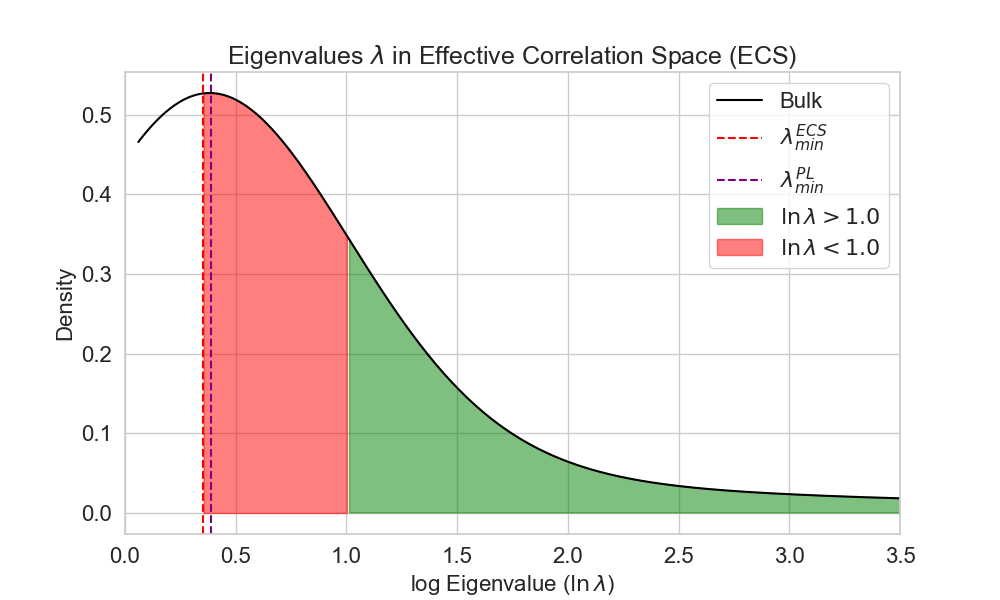
\includegraphics[width=10cm]{./img/ECS_space.png}
  \caption{The image depicts a typical
    \EmpiricalSpectralDensity (ESD) of a layer correlation matrix $\XMAT$, with \WW Power-Law (PL) exponent
    $\alpha=2.0$.%, normalized such that $\Trace{\XMAT}=\Vert\WMAT\Vert^{2}_{F}=N$.
    The green and red shaded regions depict
    eigenvalues $\lambda$ in the \EffectiveCorrelationSpace (\ECS) of $\XECS$, defined by $\lambda>\lambda_{min}^{ECS}$.
    The x-axis displays the eigenvalues on the log scale, $\ln\lambda$.
    The vertical red line is at the start of the PL tail  $(\lambda_{min}^{PL})$.
    The purple, vertical line is at the start of the~\ECS tail  $(\lambda_{min}^{ECS})$.
    The green shaded region depicts those eigenvalues where $\ln\lambda>1.0$,
    whereas the red shaded region depicts those eigenvalues where $\ln\lambda<1.0$.
    The~\ECS is defined such that the volume-preserving~\TRACELOG condition is best satisfied, i.e $\sum\ln\lambda= 0$ for $\lambda\ge\lambda_{min}^{ECS}$.
    }
  \end{center}
  \label{fig:ECS_space}
\end{figure}

Because the \Teacher ESD is most likely MHT and PL, 
if we choose $\lambda_{min}^{ECS}$ too small, and the tail extends too far into the bulk region of the ESD,
then for all practical purposes $\Det{\XECS}\ll 1$.
On the other hand, if we choose $\lambda_{min}^{ECS}$ too large,
then we only capture very large eigenvalues, and for all practical purposes $\Det{\XECS} \gg 1$.
Therefore, if we set the scale of $\XECS$ appropriately, we can choose a $\lambda_{min}^{ECS}$ such that $\Det{\XECS}=1$.
In this case, by choosing $\LambdaECSmin$ appropriately, we can estimate the expected value of
$\langle\Det{\AMATM}\rangle$  with an empirical point estimate over the \Teacher Correlation matrix, which is unity.
\begin{equation}
\label{eqn:detX}
\vert\det\XECS\vert \simeq 1 ; \quad \Trace{ \ln\XECS } = \ln\vert\det\XECS\vert \simeq 0  .
\end{equation} 

This expression can now be used in a practical calculation to define a low-rank subspace that both allows us to evaluate the HCIZ integral,
and to identify, in principle, generalizing components of the layer.
We also refer to \EQN~\ref{eqn:detX} as the \TRACELOG condition, which is technically its empirical form.
\michaeladdressed{Note by abuse of terminology.}
For example, Figure~\ref{fig:ECS_space} depicts the eigenvalues in the~\ECS for a \Typical ESD with PL $\alpha=2.0$,
(normalized such that $\Trace{\XMAT}=\Vert\WMAT\Vert_{F}=N$).
Notice that the start of the PL tail, $(\lambda_{min}^{PL})$, is very close to the start of the~\ECS tail. $(\LambdaECSmin)$,
i.e. $\Delta \lambda_{min}:=\LambdaECSmin-\LambdaPLmin\approx 0$.
Also, notice that while there are many large eigenvalues, $\ln\lambda>1.0$, there are numerous small eigenvalues as well,
$\ln\lambda<1.0$, such that the $\sum\ln\lambda\approx 0$ for $\lambda\ge\lambda_{min}^{ECS}$. In other words, the red and green shaded areas have the same measure.
Additional plots like Figure~\ref{fig:ECS_space}, generated with \WW,  can be found in Section~\ref{sxn:empirical},
in Figure~\ref{fig:mlp3-detx-gap}
as well as plots of $\Delta \lambda_{min}$ vs. the \WW PL $\alpha$ for several real-world examples,
in Figures~\ref{fig:CV_ESD_trends} and ~\ref{fig:LLM_ESD_trends}.


%\subsection{Evaluating the HCIZ Integral in the Large-$N$ Limit}
\subsection{Evaluating the Layer Quality \texorpdfstring{$(\Q)$}{Q} in the Large-\texorpdfstring{$N$}{N} Limit}
\label{sxn:matgen_evaluation_hciz}

%%%Here, we model the matrix-generalized Average ST \Quality (Squared)
%%%$\QT$ of an HCIZ integral, and in the large-$N$ limit. 
%%%\michael{Why change notation below?  I sort of like it but sort of dont.}
%%%We can write the generating function $\IZG$ (for the Total Average \Quality Squared $\mathcal{Q}^{2}$)
%%%in \BraKet notation as
%%%\begin{align}
%%%  \label{eqn:IZG_hciz}
%%%  \IZG := & \frac{1}{N}\left\langle     \exp ( N\beta \Trace{\tfrac{1}{N} \TMAT^{T}\AECS_{2}\TMAT })\right\rangle_{\AECS} 
%%%\end{align}
%%%or explicitly as an integral as
%%%\begin{align}
%%%  \label{eqn:IZG_integral}
%%% \IZG  := & \frac{1}{N}\int d\mu(\AECS) \exp ( N\beta \Trace{\tfrac{1}{N} \TMAT^{T}\AECS_{2}\TMAT })
%%%  \end{align}
%%%or, in Tanakas notation,
%%%\begin{align}
%%%  \label{eqn:IZG_tanaka}
%%% \IZG  := & \frac{1}{N}\mathbb{E}_{\AECS}\left[ \exp ( N\beta \Trace{\tfrac{1}{N} \TMAT^{T}\AECS_{2}\TMAT })\right]
%%%\end{align}
%%%where 
%%%$\langle\cdots\rangle_{A}=\int\cdots d\mu(A)=\mathbb{E}_{A}[\cdots]$
%%%are equivalent notation denoting the expected value (or average) over all \Student Correlation Matrices $\AECS$ spaning the~\ECS,
%%%$\AECS_{2}$ is a (random) $N\times N$ square (correlation) matrix, and
%%%$\TMAT$ is a (non-random) \Teacher $N\times M$ rectangular (weight) matrix.
%%%That is, $\TMAT$ the actual layer weight matrix $\TMAT=\tilde{\WMAT}$ of the model we wish to study
%%%(but also only in the span of the~\ECS).
%%%Notice also that, here,  $\beta$ is the inverse-Temperature and not the simple constant $1$ or $2$ as in \cite{Tanaka}.
%%%
%%%\nred{REPEATED AGAIN}
To generate the Average \Quality, $\QT$, we first take the large-$N$ limit of $\IZG$
\begin{equation}
  \label{eqn:IZG_limit}
  %  \IZGINF := \lim_{N\gg 1}\IZG = \lim_{N\gg 1}\ln\; \mathbb{E}_{\AECS}\left[\exp N\beta\left( \tfrac{1}{N}\Trace{ \TMAT^{\top}\AECSN\TMAT } \right)\right] ,
\IZGINF := \lim_{N \gg 1} \IZG 
= \lim_{N \gg 1}   \red{\tfrac{1}{N}}
\ln \; 
  \Expected[\AECS]{ 
    \exp\,
      N \beta \Trace{\tfrac{1}{N}\TMAT^{\top}\,\AECSN\,\TMAT}
  } 
\end{equation}
and then take the appropriate partial derivative,
analogously to how we did for $\AVGSTGE$; see Section~\ref{sxn:quality} for more details.
This gives (as in \EQN~\ref{eqn:QT_def})
\begin{align}
\label{eqn:IZG_generate_Q2}
\QT &:= \frac{1}{\beta}\frac{\partial }{\partial \ND}\IZGINF  \\ 
&\underset{\text{high-}T}{\approx}
\frac{1}{\ND}\frac{\partial }{\partial \beta}\IZGINF 
\end{align}
Notice that since we are at high-Temperature, it doesn't matter which partial derivative we take,
and we expect both results to be yield the same expression.

This HCIZ integral in \EQN~\ref{eqn:IZG_limit} can be evaluated
(i.e in the large-$N$ limit) using a result by Tanaka ---provided
the matrix $\AECSN$ is low rank, which holds when the \TRACELOG condition is satisfied.
Thus, moving forward, we will assume an
\EffectiveCorrelationSpace (\ECS) of rank $\MECS$, where $\LambdaECSmin$ is the $M^{th}$-largest eigenvalue of $\XECS$,
and defines the start of the~\ECS (and whatever branch-cut is necessary to integrate $R(z)$).

Tanaka's result for the~\ECS can be expressed as:
\begin{equation}
  \label{eqn:tanaka_result}
  \underset{N\gg 1}{\lim}\frac{1}{N}\ln
\Expected[\AECS]{\exp\left(\ND\beta \Trace{\TMAT^{\top}\AECSN\TMAT}\right)}
  =\ND\beta\sum\limits_{i=1}^{\MECS}\;\GNECSI,
\end{equation}
where the sum now only includes the eigenvalues of $\XECS$ (in the~\ECS), $\beta=\tfrac{1}{T}$
is the Inverse-Temperature, and $\LambdaECS$ is an eigenvalue of $\XECS$, the Teacher
Correlation matrix projected into the \ECS space.
$\AECSN$ is the $N \times N$ form of the \Student Correlation matrix,
with $N-M$ non-zero eigenvalues, and $\TMAT$ is the $N\times M$ \Teacher  weight matrix
(also effectively projected into the \ECS, i.e. $\TMAT=\TECS$ here).
$\GNI$ is the \GEN, defined below.
\footnote{We use the notation $\Expected[\AECS]{\cdots}$ for expected value and placed $\tfrac{1}{N}$ on the L.H.S.
to help the reader compare this to the original expressions in~\cite{Tanaka2007, Tanaka2008}.
Also,  in \cite{Tanaka2007, Tanaka2008},$\beta=1|2$, but, in fact, if one inserts $-\beta$ as an inverse temperature into the final expression, it simply factors out.}
This gives
\begin{equation}
\label{eqn:tanaka_result2}
\IZGINF = \ND\beta\sum\limits_{i=1}^{\MECS}\;\GNECSI,
\end{equation}
\michaeladdressed{State this in a self contained way, with rank assumptions, etc.}


This gives a final expression for the Average \LayerQuality (Squared) $\QT$ as
\begin{equation}
\label{eqn:Q2_result}
\QT = \sum\limits_{i=1}^{\MECS}\;\GNECSI,
\end{equation}
Note that $\QT$ is independent of $N$ and $\beta$,
and, indeed, \EQN~\ref{eqn:IZG_generate_Q2} is an equality.

The average \Quality (squared) can be expressed as a sum over
\GeneratingFunctions $\GN$, which depend only the statistical properties of the
actual \Teacher Correlation  matrix  $\XECS$ (projected into the~\ECS).
Each term in the sum, $\GNECSI$, takes the form
\begin{equation}
\label{eqn:generating_function_A}
 \GN:=\int\limits_{0}^{\lambda}R_{\AMAT}(z)dz \xrightarrow{\text{\ECS}}\int\limits_{\LambdaECSmin}^{\lambda}R_{\AECS}(z)dz
\end{equation}
where $R_{\AECS}(\LambdaECS)$ is the \RTransform from RMT,
and $\LambdaECSmin$ is the lower bound of the~\ECS spectrum.
Importantly, the \RTransform for a Heavy-Tailed ESD may have a branchcut at or near the
start of the~\ECS (as explained in Section~\ref{sxn:r_transforms}), so restricting the integrand
to start at $\LambdaECSmin$ is critical.

\charles{
  should we call $\GN$ a Generating Functiton or maybe a Norm \GeneratingFunction because the simplest result is something like a  Trace Norm ?
 }

\charles{removed section below for space reasons; see tex file}
%The \RTransform is like an inverse Greens function and is also a Cumulant generating function.
%\michael{Still to fix this par.}
%Specifically, the $R$-transform arises in RMT in the following way. 
%gWe can define the Greens function $\mathcal{G}_{A}(z)$ for any square, positive-definite matrix $\AECS$ as the Steiljes Transform of the ESD $\rho_{A}(\lambda)$.
%\michael{Clarify.}
%Following Zee~\cite{Zee:Blue}, we call $\mathcal{B}(z)$ the \BlueFunction, which is the functional inverse of $g(\AECS)$
%For example, if $\mathcal{G}_{A}(z)=XXX$ then  $\mathcal{B}(z)=YYY $.
%We can then define the $R$-Transform $R(z)$ in terms of $\mathcal{B}(z)$ as XXX.  
%\michael{What does that mean?}
%\charles{RMT has its own Cumulant generating function}

%\michael{Either modularize thias a remark, or lets give an explicit equation that we need to call for our subsequent derivation, or for others to follow up on our derivation.}
%The $R$-tramsform is commonly referred to as the Cumulant Generating Fucntion for RMT.
%However, it also has another interpretation, which is relevant here. 
%Obviously, the R-tramsform of a matrix $\AECS$ can be thought of as a modified functional inverse of the Greens function for $\AECS$,
%
%More importantly, however, if one considers the $R$-transform of the sum of two matrics $\AECS_{2}+\AECS_{2}$, then the resulting expression represents a kind of single-particle Greens function for the interacting matrices~\cite{Zee:Blue}.
%
%Most importantly, we know the $R$-transform for an HT random matrix with a PL ESD (see \EQN~\ref{eqn:R_PL}, below).

\michael{@charles: if I understand things, the following (until the end of the section) is a big shift; we are going from doing Tanaka, to justifying why we use the empirical data; we should highlight it more clearly.}
\charles{@michael: thats true}

Since we expect the best Student matrices to resemble the actual \Teacher matrices, we expect the \Student correlation matrix $\AECS$ to have similar spectral properties to our actual empirical correlation matrices $\XECS$.
That is, from the perspective of \HTSR theory and the classification into \PhasesOfTraining~\cite{MM18_TR_JMLRversion}, we expect all the $\AECS$ to be in the same phase as $\XECS$ (and, in addition, to have the same PL exponent value).   That is, 
\\
\\
\emph{We expect the \RTransform of $\AECS$ to have the same functional form as the $R$-transform of $\XECS$.}
\\
\\
If our (\Teacher) NN weight matrix exhibits a HT PL, then the tail the ESD ($\rho_{tail}(\lambda)$) of the \Student and \Teacher will both take the limiting form of a PL, with the same empirical variance $\sigma^{2}$ and (critically) the same PL exponent $\alpha$:
\begin{equation}
\label{eqn:R_PL}
  \rho_{tail}[\AECS](\lambda)\sim\rho_{tail}[\XECS](\lambda)\sim\lambda^{-\alpha}.
\end{equation}

Up until this point, our derivation of $\QT$ only depends on the \TRACELOG condition, irrespective of the exact functional form of $R(z)$,
therefore the \SETOL approach tested by examining how well the \TRACELOG condition holds for the layers in very well performing models.
We do this in Section~\ref{sxn:empirical-trace_log}.






\subsection{Modeling the R-Transform}
\label{sxn:r_transforms}

\charles{NOTE: There is some subtly here to deal woith because of the branch cuts expected in $R(z)$
  We can derive \ALPHAHAT from the R-Transform, but its a bit lengthy.
  I will also work out the R transform for the truncated power law for $\alpha=2$ and maybe $3,4$ and explain}

In this section, we explain how to select the \RTransform $R(z)$ and evaluate the~\GEN~$\GN$ under different modeling assumptions.
To apply \SETOL, the model satisfy the \TRACELOG condition--which occurs during the case of  \IdealLearning.
For most cases of NN models, the ESD are HT; and this, in practice, one usually would select $R(x)$ that reflects this. 
We analyze several cases, noting their applicability to real-world scenarios.
Most importantly,  we derive expressions that resemble the~\WW~\ALPHAHAT metric, at least formally valid
for the case $\alpha\approx 2$.

\michaeladdressed{We should note here that for some or all of these derivations we obtain results only when we have \IdealLearning.}


\subsubsection{Elementary Random Matrix Theory}
\label{sxn:r_transforms:elementary_rmt}

We beging with some useful notions definitions from \RandomMatrixTheory.
%
Using the ESD $\rho(\lambda)$, defined as
\begin{equation}
\label{eqn:rgo}
\rho(\lambda):=\frac{1}{N}\sum_{i}\delta(\lambda-\lambda_{i})  ,
\end{equation}
%
we can express the \emph{\GreensFunction} (or \emph{\Cauchy}-Stieltjes transform) by%
\footnote{Please notice our naming and sign convention in \EQN~\ref{eqn:Cz}.
\michaeladdressed{Which? Or is this the def here?}
\charles{@michael: it a sign convention. Read forward}
Some authors equate the \GreensFunction $G(z)$ with
the \Cauchy-Stieltjes transform, whereas we define $C(z)=-G(z)$.}
\begin{equation}
\label{eqn:Gz}
G(z):=\int \mathrm{d}\lambda \frac{\rho(\lambda)}{z-\lambda} .
\end{equation}
%
From $G(z)$, we can recover the ESD, $\rho(\lambda)$, using the inversion relation
\begin{equation}
\label{eqn:GzInverse}
\rho(\lambda)=\lim_{\epsilon\rightarrow 0+}\frac{1}{\pi}\mathrm{IM}(C(\lambda+i\epsilon))  ,
\end{equation}
where $\mathrm{IM}$ is the imaginary part of $G(z)$, and where the $\lim_{\epsilon\rightarrow 0+}$ means to take the limit approaching from the upper half of the complex plane.
%
The \RTransform, $R(z)$, can be defined using the Blue function $B(z)$ 
\begin{equation}
\label{eqn:Rz}
R(z):=B(z)-\frac{1}{z}  ,
\end{equation}
where the Blue function $B(z)$~\cite{Zee1996} is the functional inverse of the Greens Function $G(z)$,% 
\footnote{The Blue function was first introduced by Zee~\cite{Zee1996} to model, among other things, spectral broadening in quantum systems.
Briefly, given a deterministic Hamiltonian matrix $\mathbf{H}_{0}$, with eigenvalues $\lambda^{0}_{i}$,
one can model the spectral broadening of $\lambda^{0}_{i}$ by adding a random matrix $\mathbf{H}_{1}$ to $\mathbf{H}_{0}$:
$\mathbf{H}=\mathbf{H}_{0}+\mathbf{H}_{1}$.  
The resulting eigenvalues of $\mathbf{H}$ now contain some level of randomness, $\sigma$, i.e., $\lambda=\lambda^{0}+\sigma$.  
To model the ESD of $\mathbf{H}$, one then specifies the invididual \RTransforms for $\mathbf{H}_{0}$ and $\mathbf{H}_{1}$; the full ESD of $\mathbf{H}$
can then be reconstructed by adding the two \RTransforms together $R(z)=R_{0}(z)+R_{1}(z)$.
Zee also notes that $R(z)$  is the same as the self-energy $\Sigma(z)$ from quantum many body theory~\cite{Zee1996}.}
satisfying 
\begin{equation}
\label{eqn:GzRelation}
B[G(z)]=z  .
\end{equation}
By specifying the $R(z)$ transform, we specify the complete ESD, $\rho(\lambda)$.
Here, we are actually only interested in the tail of $\rho(\lambda)$.
%and we can accept errors in $R(z)$ that describe the bulk region inaccurately or improperly. 
That is, we can given $R(z)=R(z)_{tail}+R(z)_{bulk}$, we only need $R(z)\approx R(z)_{tail}$.
\michaeladdressed{Good point to make here, but we need to make clear that our bulk/tails are not their bulk/tails.}
\charles{@michael: who is 'they' ?  }

\charles{Describe $R(z)$ is a power series, and how we take $\int dz R(z)$ and why we restirct the integral, contours, etc}



\subsubsection{Known \RTransforms and Analytic (Formal) Models}
\label{sxn:r_transforms:known_r_transforms}

There only a few known analytic results for the explicit \RTransform $R(z)$.
Below, we review some of them, explaining what ESD they correspond to,
and what the resulting \GEN~$G(\lambda)$ would be if applied
as a model $R(x)$ in the \SETOL approach.

See Table~\ref{tab:known_r_transforms}.

\nred{Note: removed \emph{Multiplicative-Wishart} }
\begin{table}[h!]
  \centering
  \renewcommand{\arraystretch}{1.25} % Increase line spacing in table
\begin{tabular}{|c|c|c|}
  \hline
  Model & \HTSR Universality class & \RTransform $R(z)$\\  \hline
  \hline
  Discrete & Spikes & $\tfrac{1}{\MECS}\sum_{i=1}^{\MECS}\lambda_{i}$   \\ \hline
  \hline
  Wishart Models & &\\ \hline
%  Multiplicative-Wishart & HT/VHT& $\dfrac{\epsilon\phi z^2}{2 - \epsilon\phi^2 z^2}$ \\  \hline
  \InverseWishart & HT/VHT &  $\dfrac{\kappa-\sqrt{\kappa(\kappa-2z)}}{z}$  \\  \hline
   \hline
  Levy \Wigner &   & \\  \hline
  General  $(\alpha_{l}\ne 1)$ & VHT/HT  & $a+bz^{\alpha_{l}-1}$ \\  \hline
  \Cauchy $\alpha_{l}=2, \beta=0$ & $\alpha=2$ & $a - i\gamma$ \\  \hline
\end{tabular}
\caption{Known \RTransforms for different matrix models.
%  The \emph{Multiplicative-Wishart} model has two real, non-zero parameters, $\epsilon$ and $\phi$; for more details, see \cite{Pennington2017}.
  For the \emph{\InverseWishart}, as given by Bun~\cite{BunThesis}, $\kappa=\frac{1}{2}(Q-1)$ where, $q=\frac{1}{Q}=\frac{M}{N}\le 1$.
  The \emph{\LevyWigner} model describes \Wigner-like Square Random Matrices
  (as opposed to Wishart-like or Correlation Matrices), where the elements are drawn from a Levy-Stable distribution.
  The Levy-Stable $R(z)$ is parameterized by a (real) shift parameter $a$,
  a complex phase factor $b$ (that depends on 3 real parameters  $\alpha_{l}, \beta$, and $\gamma$),
  and, importantly,  a PL-like tail exponent $\alpha_{l}\in (0,2)$;
  For more details, the text, see~\cite{BJNx01_TR,BJNx06_TR,BJ09_TR}.
  \red{For our modeling purposes here, we make the association $\alpha_{l}\sim\alpha/2-2$. maybe not?}
  (Also, for simplicity, we assume the variance $\sigma=1$ for all models above, where appropriate.)
  \michaeladdressed{Is that assumption just for this table.}
  \charles{@michael: yes}
}  
\label{tab:known_r_transforms}
\end{table}

\charles{Discuss the Table briefly, and then each model in its own subsubsection.
We can create plots to show how these models can treat heavy tails, and explain the parameter fitting
}
\michael{We have five rows in the table but three subsubsxns below. How many do we have? Maybe make each a par rather than a subsubsxn.}
\charles{@michael: this is low priority, can revisit later}

\subsubsection{Discrete Model: Spikes}

Here, we consider modeling the HT tail ESD, $\rho_{tail}(\lambda)$, as a collection
of discrete spikes $\lambda_{spike}$, 
where $\lambda_{spike}\ge \LambdaECSmin$.
Here, \RTransform for the \ECS is sum of Dirac delta functions  (as opposed to using
the Inverse-Wishart (IW) or other model $R(z)$.)
This lets us compute the \LayerQuality $\Q$ in closed form in term of the Teacher weight matrix
$\TMAT=\WMAT$.

\michaeladdressed{What is the meaning of the thing we derive if the \TRACELOG condition doesn't hold? Do we have any control on it?  And what do you mean it doesn't hold? }
Let the tail of the ESD have $\MECS = M^{tail}$ eigenvalues that define the \ECS, i.e.,  
\begin{equation}
\label{eqn:spikes_model_0}
\rho_{tail}(\lambda)=\sum_{i=1}^{\MECS}\delta(\lambda-\lambda_{i}) .
\end{equation}
\michaeladdressed{Let's sync, since I don't know what that phrase means in this context, and I want to make sure we didn't introduce a confusion above.}
\charles{@michael: seriously?!  We have discussed this multiple times.  We dicussed it at dinner in New Orleans.}
The \GreensFunction $G(z)$ is then
\begin{equation}
\label{eqn:spikes_model_1}
G(z) = \int d\lambda \dfrac{ \rho_{tail}(\lambda) }{z - \lambda} =
\sum_{i} \int d\lambda \dfrac{\delta(\lambda-\lambda_{i}) }{z - \lambda} =
\sum_{i} \dfrac{1}{z-\lambda_{i}}  ,
\end{equation}
and the Blue function for each invividual term $i$ is $\frac{1}{z-\lambda_{i}}$, i.e., $B(z)=\lambda_{i}+\frac{1}{z}$. 
Now, using the additive property of the \RTransform, we can express the total $R(z)$ as the sum of the \RTransforms for the individual terms $i$, giving
\begin{equation}
\label{eqn:spikes_model_2}
R(z) =\sum_{i}\left(\lambda_{i}+ \dfrac{1}{z}\right) - \dfrac{1}{z}=
\sum_{i}\lambda_{i}  .
\end{equation}
This gives the \GEN~$\GN$ as
\begin{align}
\label{eqn:spikes_model_3} 
\GN 
&= \int_{\LambdaECSmin}^{\lambda}\sum_{i}\lambda_{i} d\lambda \\ \nonumber
&= \sum_{i}\lambda_{i} \int_{\LambdaECSmin}^{\lambda} 1 d\lambda \\ \nonumber
&= \left(\sum_{i}\lambda_{i}\right)\left(\lambda-\LambdaECSmin\right)
\end{align}
Seeing that $\LambdaECSmin$ is usually quite small, we make the approximation
\begin{align}
\GN  \approx \left(\sum_{i}\lambda_{i}\right)\left(\lambda\right)  ,
\end{align}
which gives the \QualitySquared approximately as
\begin{align}
  \label{eqn:spikes_model_4}
  \QT = \sum_{i}\GNI 
 \approx\left(\sum_{i}\lambda_{i}\right)^{2}  .
\end{align}
We now see that we can define $\Q:=\sqrt{\QT}=\sum_{i}\lambda_{i}$ is what we call a Tail Norm.

\nred{CHECK FOR ERRORS PLEASE; Also ?  not really a Trace norm since this is defined over singlular values ?}
\michael{MM TO DO: connect to trace norm; the singular value thing should be okay.}
\charles{@michael: then do it}


%The Multiplicative-Wishart (MW) model  has two real, adjustable parameters $\epsilon,\phi$.
%It treates $\mathbf{X}$ as resulting from product of random matrices, and is good for modeling an ESD with a very heavy tail.
%It has been used previously to model the heavy tail of the Hessian matrix in NNs\cite{Pennington2017}
%This model would work better for fitting HT ESDs that decay slower than a TPL.  We will not consider
%this model further here and leave this for future work.

%We will work out  the full details, going from $\rho(\lambda)\rightarrow G(z)\rightarrow R(z)\rightarrow \QT$


\subsubsection{Inverse-Wishart Model of \IdealLearning}

Here, we consider the \InverseWishart (IW) model.
The IW model treats the ESD of $\mathbf{X}^{-1}$ when the ESD of $\mathbf{X}$ itself is MP.
As a parametiric model, it can be quite effective at treating VHT and HT (or \FatTailed) ESDs when the far tail decays very rapidly, like a TPL, and/or for $\alpha\le 4$.
To do this, one simply considers the parameters $\kappa$ as an adjustable paremeter.
\michaeladdressed{Give a functional form, with $\kappa$ appearing.}
\charles{@michael: do it yourself or don't suggest it}
%
It is an excellent model for the ESD when $\alpha=2.0$ (and $Q=2$).
Using this model, we can derive an expression for the \HTSR \ALPHAHAT \LayerQuality metric,
$\ALPHAHATEQN :=\ALPHAHATLONG)$ as a leading order term in the final expression for $\log_{10}\QT$.

This model 


\begin{figure}[h]
    \centering
    \subfigure[IW Distribution, $\kappa=0.25$]{ 
      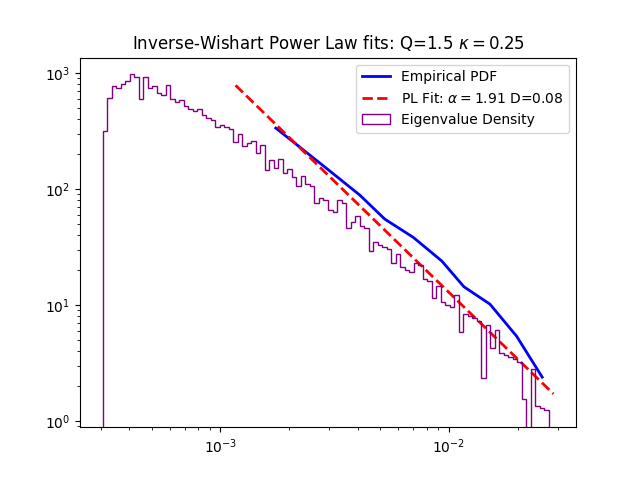
\includegraphics[width=5cm]{./img/IWplotQ1.5.png}
      \label{fig:IWplotQ15}                                                                                                      
    }                               
      \subfigure[IW Distribution, $\kappa=1.25$]{ 
      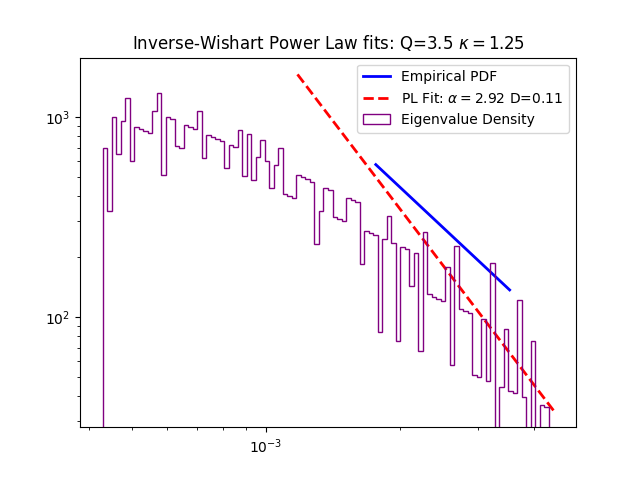
\includegraphics[width=5cm]{./img/IWplotQ3.5.png}
      \label{fig:IWplotQ35}                                                                                                      
      }
      \caption{Example Inverse-Wishart (IW) distributions for $\kappa=0.25$ and $\kappa=1.25$,  along with Power Law (PL) fits of the generated distribution. Plots on Log-Log scale.}
  \label{fig:IWplots}                                                                                                      
\end{figure}   

In Figure~\ref{fig:IWplots}, we fit some \Typical layer ESDs to an IW distribution.
When $\kappa=0.25$, the fitted $\alpha=1.91$, and the fit is a reasonably accurate model of the underlying Power Law
distribution and the ~\WW PL fit.
For  $\kappa=1.25$, the fitted $\alpha=2.92$ is larger, but the fit is not as good as a
model. Generally speaking, $\alpha$ scales with $\kappa$, but the  free cumulants scale inversely with $\kappa$.
So smaller $\alpha$ will give larger free cumulants and therefore a larger $\QT$.
Importantly, as seen in Figure~\ref{fig:IWplotQ15}, for $\alpha=\simeq 2.0$, the IW model (with $\kappa=0.25$)
is an effective simple model to illustrate the \SETOL case of \IdealLearning.
\michaeladdressed{Maybe this par and fig elsewhere; or at end of subsubsxn.}
\charles{@michael: low priority; can revisit}

\begin{figure}[t]
    \centering
    \subfigure[IW $R(z)$, real $z$.]{
        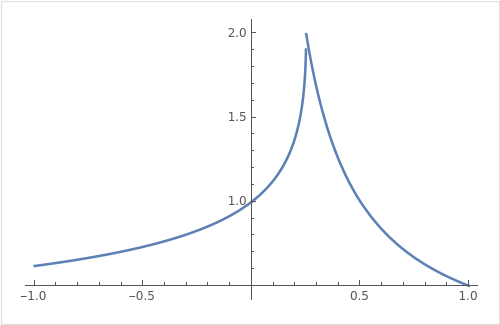
\includegraphics[width=4cm]{./img/R.png}
        \label{fig:IW_R}
    }
    \subfigure[Branch cut at $z=\kappa/2$]{
        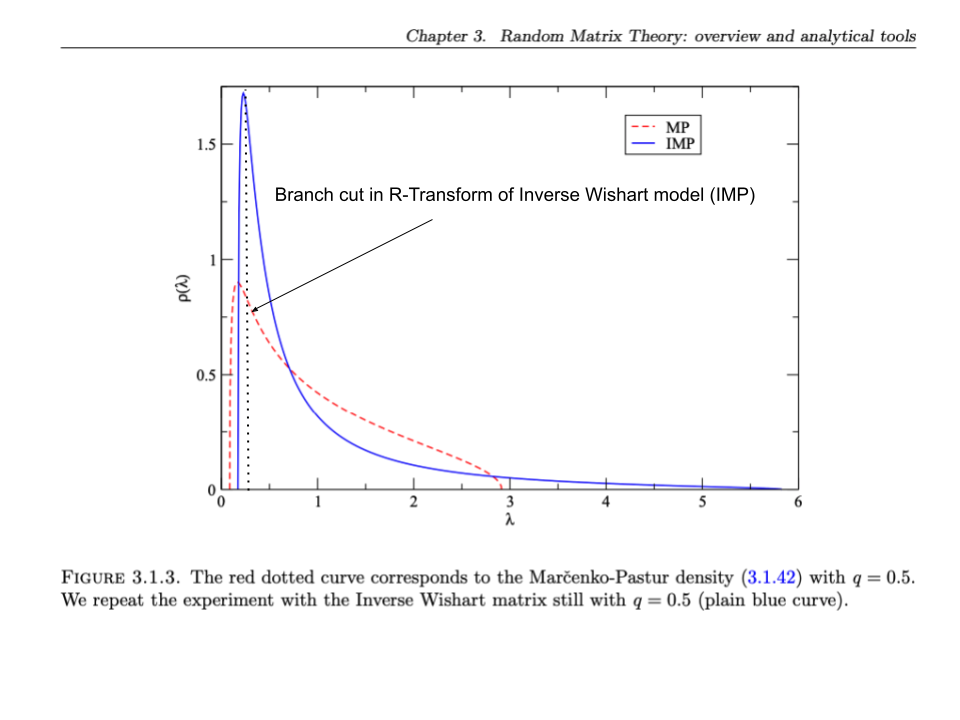
\includegraphics[width=4cm]{./img/branch-cut.png}
        \label{fig:IW_branch_cut}
    }
    \caption{(a) The function $R(z)$ of the Inverse Wishart model, with a singularity at $z = \kappa/2$. (b) The branch cut in the empirical spectral density, corresponding to the tail for $\kappa = 0.5$.}
    \label{fig:R_branch_cut_combined}
\end{figure}

Lets consider $R(z)$ for the \InverseWishart model, denoted $R(z)[IW]$.
To integrate this function, we require that it be analytic.
At first glance, it may seem that that $R(z)[IW]$ is not analytic because it
has a pole at $z=0$ and because the square-root term $\sqrt{\kappa(\kappa-2z)}$  creates branch
cut at and $z=\kappa/2$ (and $z=\infty$).
Figure~\ref{fig:R_branch_cut_combined} presents this in two ways:
Figure~\ref{fig:IW_R} shows the R-transform $R(z)[IZ]$ for real $z$, highlighting its singular behavior and the location of the branch cut at $z = \kappa/2$; and
Figure~\ref{fig:IW_branch_cut} shows the corresponding branch cut in the ESD of the Inverse Wishart model (for $\kappa = 0.5$).
We select the branch cut starting at $z=\kappa/2$ and ending at $z=\infty$,
which allows us to at least formally defined the integral along the physically meaningful part of the ESD:
\begin{equation}
\label{eqn:IW_model_1} 
\GN[IW] := \int_{\LambdaECSmin}^{\lambda} R(z)[IW] dz  ,
\end{equation}
noting that we expect $\LambdaECSmin\ge\kappa/2$.
\michael{Why do we have this par, if we are using quality squared. I need to understand.}
\charles{@michael: whats the issue ?}

It turns out, however, that due to the branch cut in $R(z)[IW]$,
the function $\GN[IW]$ is not analytic in the domain we need. 
To correct for this, we will instead model the \LayerQualitySquared using the modulus of $\GN[IW]$,
\begin{equation}
\label{eqn:IW_model_1} 
|\GN[IW]| := \sqrt{\GN[IW]^{*}\GN[IW]}
\end{equation}
where $\GN[IW]^{*}$ is the complex conjugate of $\GN[IW]$.
This is somewhat involved, so we present the full calculation in Appendix~\ref{sxn:IW}
\michael{MM TO DO: Go through.}
\michael{Are we going to mention the result here since we will use it?}


Figure~\ref{fig:InverseWishartGx} plots $|\GN[IW]|$ on Lin-lin and Log-log plots, on the range $\lambda\in(0.25, 100)$, and fits the it to a PL. 
The fit follows the general trend of the function, but it is not terribly accurate.
Still, from this plot, we can see that the \LayerQualitySquared has the same general trend as $\ALPHAHAT$ and/or a Shatten Norm.

\begin{figure}[t]
  \centering
  \subfigure[$|\GN\lbrack IW\rbrack|$ Lin-lin plot and PL fit]{
    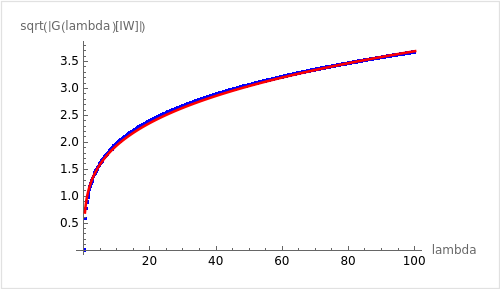
\includegraphics[width=0.45\textwidth]{./img/Gx.png}
        \label{fig:GxPlot}
    }
    \subfigure[$|\GN\lbrack IW\rbrack|$ Log-log plot and PL fit]{
        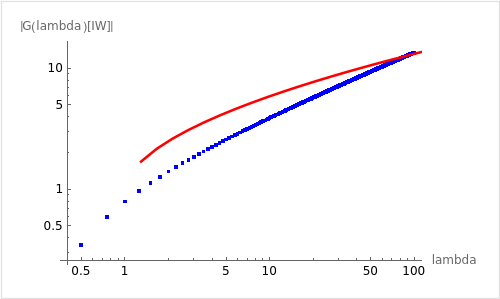
\includegraphics[width=0.45\textwidth]{./img/logGx.png}
        \label{fig:LogLogGxPlot}
    }
    \caption{Behavior of $\GN[IW]$ for the Inverse Wishart (IW) model,
       with a Power Law (PL) fit (red), $|\GN[IW]|\approx 1.138 \lambda^{0.539}$.
      (a)  Lin-lin plot. (b) Log-log plot.
}
    \label{fig:InverseWishartGx}
\end{figure}

%
%\begin{figure}[t]
%    \centering
%    % Subfigure (a): G(x) Plot
%    \subfigure[Inverse Wishart $\GN$]{
%        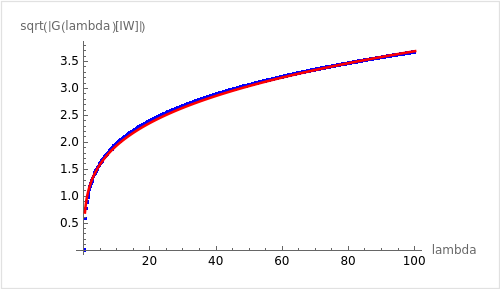
\includegraphics[width=0.45\textwidth]{./img/Gx.png}
%        \label{fig:GxPlot}
%    }
%    % Subfigure (b): Log-log plot and power-law fit
%    \subfigure[Log-log plot and power-law fit]{
%        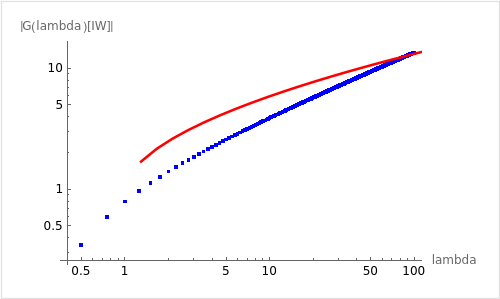
\includegraphics[width=0.45\textwidth]{./img/logGx.png}
%        \label{fig:LogLogGxPlot}
%    }
%    \caption{Behavior of $\GN$ for the Inverse Wishart (IW) model. (a) $\GN$ lin-lin plot. (b) Log-log plot of $\GN$ with a Power Law (PL) fit, $\GN\sim 2.8\lambda^{-3.0}$ }
%    \label{fig:InverseWishartGx}
%\end{figure}
%
%Given an analytic expression for $\GN$ (and $\kappa=0.25$), we can plot the $\GN$ as a function of $\lambda$,
%and then fit this to a Power Law; this is depicted in Figure~\ref{fig:InverseWishartGx}.
%The resulting fit gives $\GN\simeq 2.8\lambda^{3.0}$.
%We can now associate $\ALPHAHAT$ with $\log_{10}\QT$ by keep the leading order term
%$(\lambda_{max}=\LambdaECS_{max}$)
%
%\begin{align}
%  \label{eqn:IW_alphahat}
%  \ALPHAHATEQN:=\ALPHAHATLONG\approx\log_{10}\QT=\log_{10}\sum_{\LambdaECS}\GNI\approx\log_{10}\mathcal{G}(\lambda_{max}\sim (\alpha+1)\log_{10}\lambda_{max}
%\end{align}
%So for $\alpha=2.0$, $\log_{10}\QT\sim (\alpha+1)\log_{10}\lambda_{max}$, which is very close to $\alpha\log_{10}\lambda_{max}$. QED.


\subsubsection{Levy-Wigner Models and the \ALPHAHAT Metric}

Here, we consider Levy-Wigner Models.
We show how to obtain the \WW~\ALPHAHAT metric by modeling the near VHT cases with an approximation to a Levy distribution at $\alpha\approx 2$.  

We do this because the~\ALPHAHAT metric has been developed to adjust for \SCALE anomalies that arise from issues like \CorrelationTraps,
making \ALPHA smaller than expected.
The  \LevyWigner (LW) model treats  $\mathbf{X}$ as if it were a \Wigner matrix (and not actually a correlation  matrix), and the $\alpha$ is different but related to $\alpha$ above in \EQN~\ref{eqn:rhoX}.
The ESD follows a Levy-Stable distribution, where $a$ is a shift parameter, and $b$ is a complex phase factor depending on 2 real factors, $\beta$ and $\gamma$.
Strictly the ESD for an LW model, $\rho_{LW}(\lambda)$, is defined by its characteristic function (i.e., the Fourier Transform of $\rho_{LW}(\lambda)$), but
we can note that the ESD is VHT, $\rho_{LW}(\lambda)\sim\lambda^{-\alpha-1}$, and that when $\alpha_{l}\approx 1$, the ESD resembles a PL HT ESD with $\alpha\approx 2$.

For case of \IdealLearning,  we choose to \emph{model} the \RTransform of our Fat-Tailed HT ESDs as
\begin{equation}
\label{eqn:LW_model_0} 
R(z)[HT] = bz^{\alpha-1},\;\alpha\simeq 2
\end{equation}
where $b$ is an unspecified constant (possibly negative and/or complex).
\michael{We need to clarify. Are we saying that we do PM instead of LW here.}
Notice that when $\alpha\approx 2$, our model is close to the LW model, $R(z)[HT]\approx R(z)[LW]$
(and gives a \Cauchy distribution if we choose $b=a-i\gamma$).

Integrating $R(z)[HT]$, and (as above) taking the approximation $\LambdaECSmin\sim 0$, we obtain (formally)
\begin{equation}
\label{eqn:LW_model_1} 
\GN[HT] = \tfrac{b}{\alpha} \lambda^{\alpha}  .
\end{equation}
%
If we now choose $b=\alpha=2$, then  $\QT$ takes the form of a Shatten Norm (squared)
\begin{equation}
  \label{eqn:LW_model_2}
  \QT = \tfrac{1}{\MECS}\sum_{i}\lambda^{\alpha}  .
\end{equation}
%
Taking the logarithm of $\GN[HT] $, we obtain
\begin{equation}
\label{eqn:LW_model_3} 
\log \GN[HT] =  \log\tfrac{b}{\alpha} +\tfrac{\alpha}\log\lambda
\end{equation}

As with the \InverseWishart (IW) model, we can derive a formal expression for $\ALPHAHAT$ using the LW model.
To do so, let us approxmate $\QT$ by the largest term in the sum over $\GN$, and then let $\lambda=\lambda_{max}$, giving
\begin{equation} 
\label{eqn:LW_model_4} 
\ALPHAHATEQN = \log_{10} \QT \approx  \alpha\log\lambda_{max}   .
\end{equation}
We present this as a formal example, noting that is slightly different from the result for the IW model, Eqn.~\ref{eqn:IW_alphahat}. 
We do not claim this is a valid empirical model, as we have not attempted to fit a real-world ESD to Levy-stable distribtion.  
\michael{Let's sync on the rationale here, since I'm not sure what is being said.}
We leave this to a future study, noting, however, there has been some work doing such fits~\cite{li2024exploring}.

Ideally, we would like to have an rigorous expression for $R(z)$ not just
in the case of \IdealLearning but also for the entire \FatTailed Universality class.
This is non-trivial to obtain and we will attempt this in a future work.
Fow now, we will take a different approach, and evaluate $R(z)$ explicitly using numerical techniques.



\newpage
\section{Empirical Studies}
\label{sxn:empirical}

In this section, we present empirical results. 
Our goals are to justify key technical claims, including key assumptions underlying our \SETOL approach, and to illustrate the behavior of \SETOL with respect to various parameters and hyperparameters.
Importantly, it is \emph{not} our goal to demonstrate that layer PL exponent~\ALPHA~and~\ALPHAHAT~perform well for diagnostics and predicting model quality for SOTA NN models, as that has been demonstrated previously~\cite{MM20a_trends_NatComm,MM21a_simpsons_TR,YTHx22_TR}.
% (using just the \HTSR \Phenomenology).

Since the \SETOL theory presented in Section~\ref{sxn:matgen} is (effectively) a single layer theory,
in order to carefully test (as opposed to simply use) \SETOL, we need to limit the degree of inter-layer interactions present in the model.
%%(For example, in one series of experiments, described below, all layers in the model are trained; and we then compare and contrast this with the case where only one layer was trained, and all other layers remained frozen with their random initializations.) 
To do so, we consider a three-layer \MultiLayerPerceptron (MLP3), trained on MNIST~\cite{MNIST1998}. 
We refer to the hidden layers as ``FC1 and ``FC2. Their output sizes and parameter counts are shown in 
Table~\ref{tab:mlp3}.

\begin{table}[h]
\begin{center}
        \begin{tabular}{| c | c | c | c |}
                \hline
                Layer & Units & Weight Parameters           & $\%$ of total \\ \hline \hline
                FC1   &   300 & $768 \times 300 = 230,700$  & $88.2\%$      \\ \hline
                FC2   &   100 & $300 \times 100 = 30,000$   & $11.4\%$      \\ \hline
                out   &    10 &  $10 \times 100 = 1000$     & $0.38\%$      \\ \hline
        \end{tabular}
\end{center}
\caption{Dimensions of each FC layer in the MLP3 model, along with weight matrix parameter count and fraction of the 
total.}
\label{tab:mlp3}
\end{table}

The following are the main topics we consider.

\begin{enumerate}[label=6.\arabic*]
\item
\textbf{\ModelQuality: \HTSR \Phenomenology.}
The \HTSR \Phenomenology provides a metric of model quality in the form of the PL exponent $\alpha$.%
\footnote{Prior work has shown that the \ALPHAHAT metric $(\hat{\alpha})$ accurately describes variations in model 
quality as a function of architecture changes~\cite{MM21a_simpsons_TR}. Since we do not vary the depth of the model in 
our evaluations, the \ALPHA metric ($\alpha$) is of interest in this setting.} 
In particular, smaller values of $\alpha$ (e.g., 
%%provided $\alpha$ is not spuriously low, as discussed in Section~\ref{sxn:HT_ESDs}, then 
values of $\alpha$ closer to $2$ than $3$ or $4$) should correspond to better models, e.g., having smaller test errors; and
a minimal error should be obtained when $\alpha=2$.
See Section~\ref{sxn:empirical-test_acc}.
\item 
\textbf{\EffectiveCorrelationSpace.}
The \SETOL theory is based on the notion of an \EffectiveCorrelationSpace, in which the learning and generalization occurs. 
This is the low-rank subspace $\mathbf{W}^{\EFF}$ of each layer $\mathbf{W}$ that approximates the teacher $\mathbf{T}$.
In particular, 
our measure of model quality should be restricted to $\mathbf{W}^{\EFF}$.
The \EffectiveCorrelationSpace can be identified from the tail of the ESD, $\rho_{tail}(\lambda)$, and it can be chosen according to one of several related Model Selection Rules.
See Section~\ref{sxn:empirical-effective_corr_space}.
\item 
\textbf{Evaluating the \TRACELOG  Condition.}
In the \HTSR \Phenomenology, when a model is very well-trained, the layer PL exponent $\alpha\simeq 2$.
In the \SETOL theory, when a model is very well-trained, the eigenvalues in the tail will satisfy the Empirical \TRACELOG  Condition, given in \EQN~(\ref{eqn:detX}).
% \michael{We should probably be citing \EQN~(\ref{eqn:logTraceNorm}), or wherever we give it a name, consistently.}
% \chris{Agree we should only cite one equation for this purpose for consistency, but I like \ref{eqn:detX} for this 
% because its easier to interpret numerically. I checked and this (was) the only place where this equation was 
% referenced, so I added another reference in the Section itself.}
In Section~\ref{sxn:empirical-trace_log}, we provide a detailed analysis of this effect.
\item
\textbf{Computational Model Qualities.}
In Section~\ref{sxn:empirical_comp_r_transforms}, we empirically compare the HTSR layer-quality exponent $\alpha$ against the computational \RTransform-derived metric $\QT$ on fully trained MLP3 models. We show that for the FC1 layer, $\QT$ closely tracks $\alpha$ with small error bars and the expected batch-size trend, whereas for FC2, $\QT$ exhibits much larger variability—demonstrating that $\alpha$ provides a more stable and robust measure of layer quality.  
\item
\textbf{\CorrelationTraps.}
Recall, from Section~\ref{sxn:Traps}, that if a layer weight matrix $\mathbf{W}$ has a \CorrelationTrap
(and, in particular, those arising from SGD training with very large learning rates)
then it is likely that the test (and train) accuracy will be degraded, and $\alpha$ will drop below its optimal value. 
See Section~\ref{sxn:empirical-correlation_trap} for an empirical demonstration of this.
\item 
\textbf{Overloading and Hysteresis Effects.}
The experiments described so far validate that \SETOL makes valid predictions in the $\alpha \gtrsim 2$ range.
Beyond that point, \SETOL only predicts ``atypicality, in the sense of spin glass theory~\cite{nishimori01}. 
See Section~\ref{sxn:hysteresis_effect} for an examination of how the MLP3 behaves when it is pushed further out of that range of validity, e.g., by training only one layer, while keeping the others frozen. In particular, we compare results when a single layer is either over- vs under-parameterized.
\end{enumerate}

\noindent
We trained the MLP3 model independently, using both the Tensorflow 2.0 framework (using the Keras api, and on Google Colab) and pytorch, with the goal of consistent, reproducible results.
Each setting of batch size, learning rate, and trainable layer was trained with $5$ separate starting random seeds, and error bars shown in plots below represent one standard deviation taken over these $5$ random seeds. 
Each training run used the same early stopping criteria on the train loss: training was halted when train loss did not decrease by more than $\Delta E_{train}=0.0001$, over a period of $3$ epochs. 
In doing so, each model was trained with a different number of epochs; and, at the end, the best weights were chosen for the model.
See Appendix~\ref{sxn:appendix_MLP3details} for more details on the MLP3 model and the training setup.
We provide a Google Colab notebook with the exact details, allowing the reader to reproduce the results as desired.

\michael{MM TO DO: make sure the following comment is mentioned earlier, not here.}
The dominant generalizing components of $\mathbf{W}$ reside in $\mathbf{W}^{\EFF}$ such that it captures the functional contribution of $\mathbf{W}$ to the NN; and thus
\charles{FINISH THOUGHTS HERE}



\subsection{\HTSR Phenomenology: Predicting Model Quality via the \ALPHA metric}
\label{sxn:empirical-test_acc}

\begin{figure}[t]
  \center
  \subfigure[Batch size experiment]{
    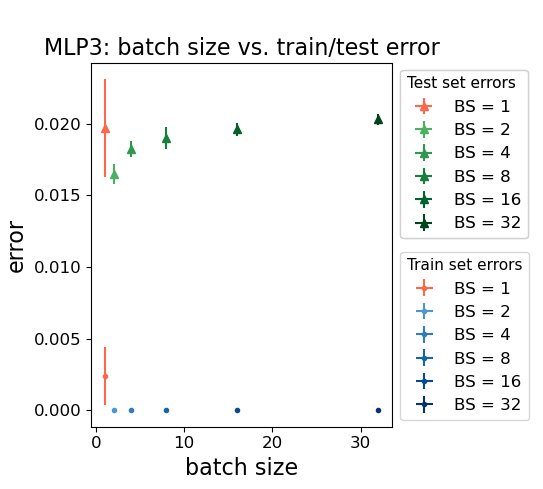
\includegraphics[width=6cm]{img/model_quality/mlp3_error_by_BS.png}
    \label{fig:mlp3-accuracies-bs}
  }
  \subfigure[Learning rate experiment]{
    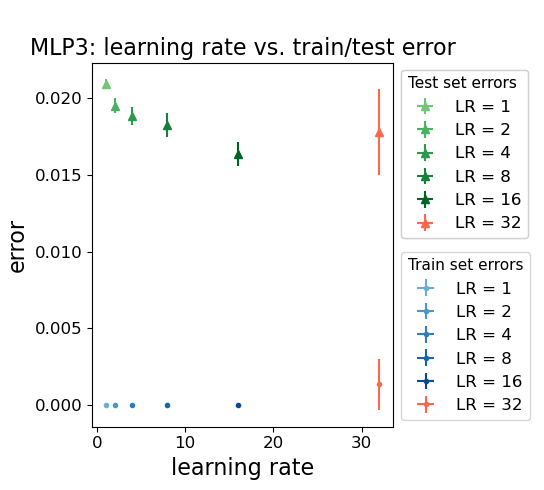
\includegraphics[width=6cm]{img/model_quality/mlp3_error_by_LR.png}
    \label{fig:mlp3-accuracies-lr}
  }
  \caption{Train / test errors in the MLP3 model as a function of batch size, and learning rate. Observe the inverse relationship between batch size (a) and learning rate (b). As batch size decreases, test error generally decreases, until batch size reached $bs=1$. Similarly, as learning rate increases, test error decreases until $lr=32\times$ the SGD default value of $0.01$.
  }
  \label{fig:mlp3-accuracies}
\end{figure}

Here, we want to determine how the quality of our MLP3 model varies with the \ALPHA metric. 
From previous work~\cite{MM20a_trends_NatComm,MM21a_simpsons_TR,YTHx22_TR}, we expect that \ALPHA metrics for the FC1 and FC2 layers should be well-correlated with the test accuracy, while varying some suitable training knob, such as learning rate or batch size, that can modulate the test accuracy.% 
\footnote{Since we do not change the depth of the model here, we expect the \ALPHA metric to follow the \ALPHAHAT metric, also predicting the test accuracies~\cite{MM21a_simpsons_TR}.}

In doing this, the goal is not to achieve \Thermodynamic equilibrium,
but, instead, by using a common stopping rule, to simulate 
in more realistic situations where models may not have fully converged.   This  allows us to test the theory outside of
its more limited apparent range of validity, 
thereby demonstrating the robustness of \SETOL.

We vary the batch size from small to large, i.e., $bs\in[1,2,4,8,16,32]$, following the setup of previous work on the \HTSR~\Phenomenology~\cite{MM18_TR_JMLRversion}. 
We expect similar effects by varying the learning rate, as it is known that small batch sizes correspond directly to large learning rates~\cite{SKYL17_TR,WT11}. 
Thus, we conducted a second set of experiments where the learning rate was varied by a factor of 
$[1\times,2\times,4\times,8\times,16\times,32\times]$, relative to the SGD default value of $0.01$. 
Adjusting the learning rate or batch size allows us to systematically vary the layer PL exponent $\alpha$ between roughly $2$ and $4$, i.e., within the range in which \SETOL should make the most reliable predictions. 
As an added benefit, it also allows us to use the very small batch size of $1$ to force the model into a state of over-regularization, which we also analyze below.


%%(In the HTSR \Phenomenology and the $5+1$ Phases-of-Training, and with how \WW~currently fits the ESDs, and barring additional spurious effects, this over-fitting regime corresponds to \VeryHeavyTailed (VHT) ESDs, with $\alpha<2$, which corresponds to a different HT \Universality class than $\alpha \in [2,4]$~\cite{MM18_TR_JMLRversion}.)

Consider Figure~\ref{fig:mlp3-accuracies}, which plots the final train and test accuracies as a function of the hyperparameter (batch size or learning rate) used during training for the MLP3 model.
Figure~\ref{fig:mlp3-accuracies-bs} varies batch size, and Figure~\ref{fig:mlp3-accuracies-lr} varies learning rate.
Recall that error bars represent one standard deviation taken over $5$ independent starting random seeds. 
In Figure~\ref{fig:mlp3-accuracies-bs}, we see that by decreasing the batch size ($bs$), and holding other knobs constant, we can systematically improve the train and test accuracy, up to a point. 
In particular, for $bs \ge 2$, both the test and train accuracies increase with decreasing batch size, consistent with previous work~\cite{MM18_TR_JMLRversion}.
Further decrease beyond $bs=2$ leads to \emph{lower} model quality, i.e., larger error and larger error variability.
In Figure~\ref{fig:mlp3-accuracies}, we see that increasing the learning rate ($lr$) by a factor $x$ has an exactly analogous effect as decreasing the batch size by $1/x$.% 
\footnote{One could, of course, mitigate this by fiddling with other knobs of the training process, but that is not our goal.  Our goal here is not to use a toy model to demonstrate the properties and predictions of \SETOL.}

\begin{figure}[t]
    \centering
    \subfigure[$\alpha_{FC1}$]{
        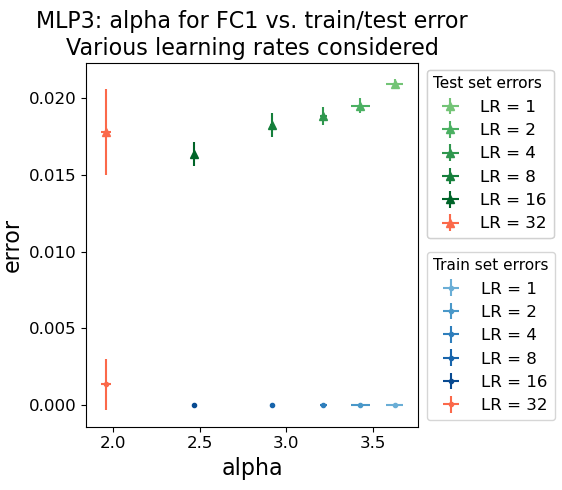
\includegraphics[width=6cm]{img/model_quality/mlp3_alpha_FC1_by_LR.png}
        \label{fig:mlp3-alpha-fc1-by-lr}
    } 
%    \subfigure[$\Delta \lambda_{min}$ FC1]{
%        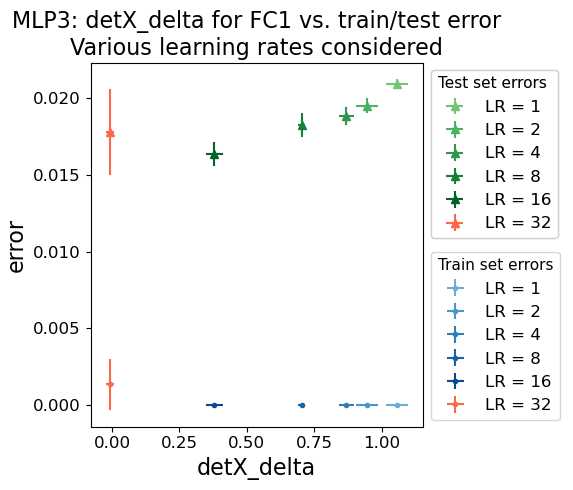
\includegraphics[width=6cm]{img/model_quality/mlp3_detX_Delta_FC1_by_LR.png}
%        \label{fig:mlp3-detx-delta-fc1-by-lr}
%    } \\
    \subfigure[$\alpha_{FC2}$]{
        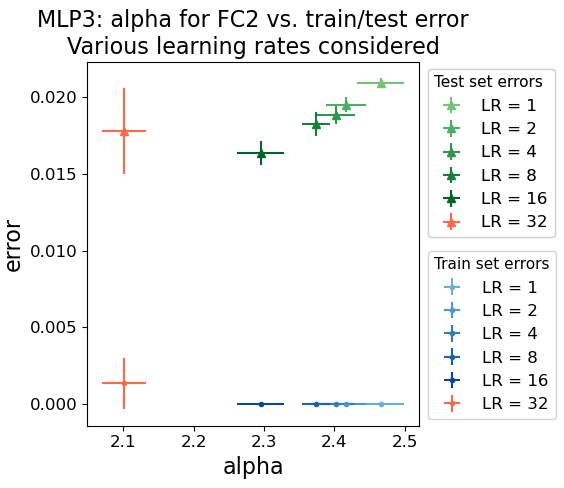
\includegraphics[width=6cm]{img/model_quality/mlp3_alpha_FC2_by_LR.png}
        \label{fig:mlp3-alpha-fc2-by-lr}
    } 
%    \subfigure[$\Delta \lambda_{min}$ FC1]{
%        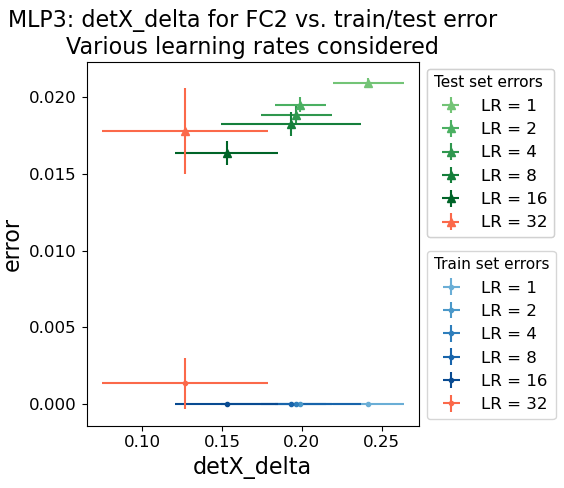
\includegraphics[width=6cm]{img/model_quality/mlp3_detX_Delta_FC2_by_LR.png}
%        \label{fig:mlp3-detx-delta-fc2-by-lr}
%    }  

    \caption{
            Train / test errors in the MLP3 model in the {\bf \emph{\LearningRate}} experiment as a function of $\alpha_{FC1}$ (a) and $\alpha_{FC2}$ (b). 
            Observe the regular downward progression of $\alpha$ and error as the learning 
            rate increased in both (a) and (b). When learning rate was $32\times$, (shown in red), $\alpha_{FC1}$ fell 
            below $2$, coinciding with a drastic increase in both train and test error. The results here almost 
            perfectly replicate those of the Batch Size experiment, shown in Figure~\ref{fig:mlp3-alphas-bs}.
              for Figure~\ref{fig:mlp3-alphas-bs}.}
 \label{fig:mlp3-alphas-lr}
\end{figure}

The transition between $lr=16\times$ (or $bs=2$), which is locally optimal for the setting of other hyperparameters, and $lr=32\times$ normal (or $bs=1$), which is not, provides a demonstration of a distinct change in the behavior of \ALPHA, concordant with the sudden increase in the error and error variability. 
To explore this in the context of \SETOL, consider Figure~\ref{fig:mlp3-alphas-lr} and Figure~\ref{fig:mlp3-alphas-bs}, which plot error as a function of \ALPHA, for different learning rates and batch sizes, respectively.

Figure~\ref{fig:mlp3-alphas-lr} plots the \ALPHA metrics $\alpha_{FC1}$ and $\alpha_{FC2}$, as learning rate is varied, demonstrating that both metrics are well-correlated with the test accuracies, for all learning rates less than $16\times$ normal. 
In particular, as we drive \ALPHA in FC1 down to an \Ideal value of $\alpha\simeq 2$, the test error decreases monotonically (Figure~\ref{fig:mlp3-alpha-fc1-by-lr}).
Beyond that point, further decrease of the batch size sees \ALPHA decrease below its \Ideal value of $2$ in the FC1 layer.
This corresponds not only with \emph{higher errors}, but also with \emph{larger error bars}, on both train and test error. 
The dramatic increase in train error and train error variability is particularly telling, because it suggests that when 
$\alpha_{FC1}$ passes below $2$, the model enters into a ``glassy state, and is unable to relax down to $0$ train error.

In Figure~\ref{fig:mlp3-alpha-fc2-by-lr}, we consider \ALPHA for FC2, and we see that $\alpha_{FC2}$ approaches $2$, but 
does not reach it, even for $lr=32\times$. This failure to achieve $\alpha_{FC2} \approx 2$, along with the much greater size 
of FC1, (See Table~\ref{tab:mlp3},) suggests that FC1 is the critical layer for the models performance. 
This also highlights some of the interplay between the layers, (which is not captured by a single layer theory) -- as $\alpha_{FC1}$ has narrow error bars throughout, $\alpha_{FC2}$ shows much more variation by way of its wider error bars. 
Thus, while model accuracy kept improving as learning rate increased up to $16\times$, this was likely driven by a better $\alpha_{FC1}$, more than by $\alpha_{FC2}$. 

In Figure~\ref{fig:mlp3-alphas-bs}, we consider batch size, and we see a near identical replication of these results, in terms of the relation of train error, test error and \ALPHA in the two layers. 
Consequently, the remainder of the experiments will focus on the learning rate experiment, as both produced substantially the same results.

\begin{figure}[t] %[h]
    \centering
    \subfigure[$\alpha_{FC1}$]{
        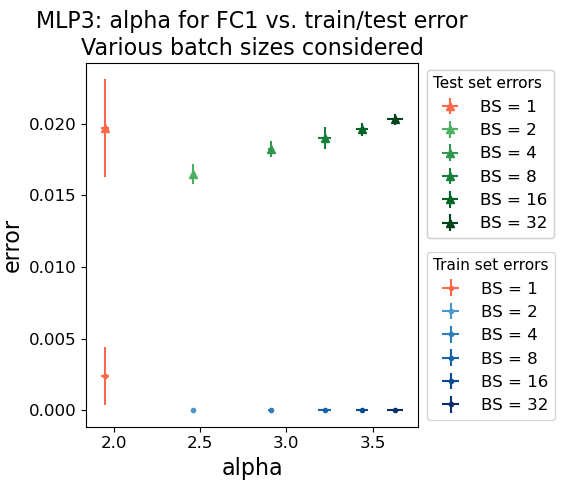
\includegraphics[width=6cm]{img/model_quality/mlp3_alpha_FC1_by_BS.png}
        \label{fig:mlp3-alpha-fc1-by-bs}
    } 
%    \subfigure[$\Delta \lambda_{min}$ FC1]{
%        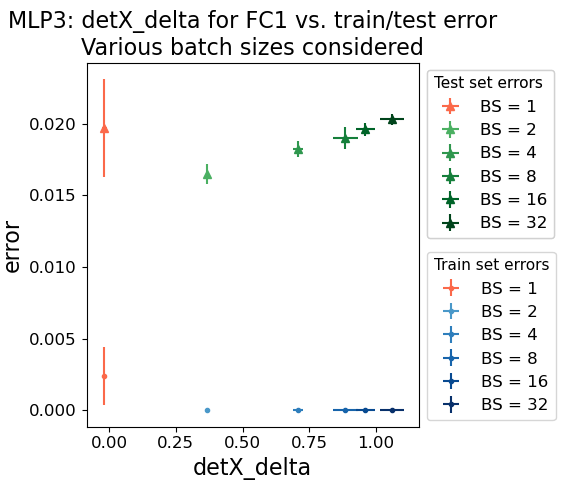
\includegraphics[width=6cm]{img/model_quality/mlp3_detX_Delta_FC1_by_BS.png}
%        \label{fig:mlp3-detx-delta-fc1-by-bs}
%    } \\
    \subfigure[$\alpha_{FC2}$]{
        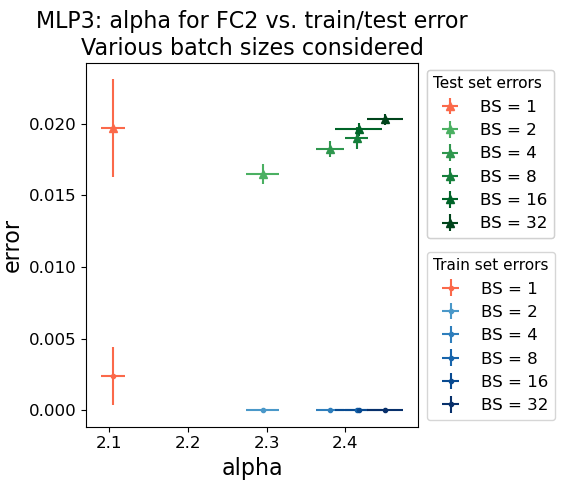
\includegraphics[width=6cm]{img/model_quality/mlp3_alpha_FC2_by_BS.png}
        \label{fig:mlp3-alpha-fc2-by-bs}
    } 
%    \subfigure[$\Delta \lambda_{min}$ FC1]{
%        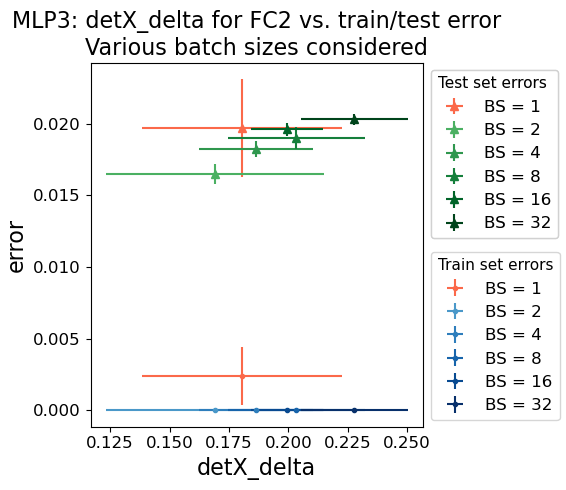
\includegraphics[width=6cm]{img/model_quality/mlp3_detX_Delta_FC2_by_BS.png}
%        \label{fig:mlp3-detx-delta-fc2-by-bs}
%    }  

    \caption{
            Train / test errors in the MLP3 model in the {\bf Batch Size} experiment as a function of $\alpha_{FC1}$ 
            (a) and $\alpha_{FC2}$ (b). Observe the regular downward progression of $\alpha$ and error as the batch size
            decreased in both (a) and (b). When batch size was $1$, (shown in red), $\alpha_{FC1}$ fell below $2$, 
            coinciding with a drastic increase in both train and test error. The results here almost perfectly 
            replicate those of the \LearningRate experiment, shown in Figure~\ref{fig:mlp3-alphas-lr}.
    }
 \label{fig:mlp3-alphas-bs}
\end{figure}





\subsection{Testing the Effective Correlation Space}
\label{sxn:empirical-effective_corr_space}

Here, we will address the question: 
\begin{quote}
How shall we \emph{test the assumption} of the \EffectiveCorrelationSpace?
\end{quote}
Recall that the \SETOL theory estimates model quality by evaluating the ST \GeneralizationError as an integral over the theoretical training data $\boldsymbol{\xi}$.
This integral assumes each layer weight matrix can be replaced with an effectively lower rank form, i.e., $\mathbf{W}\rightarrow\mathbf{W}^{\EFF}$, corresponding to the span of the eigencomponents defined by the tail of the ESD, $\rho_{tail}(\lambda)$. 
In the \HTSR \Phenomenology, the tail is defined by the fact that $\rho_{tail}(\lambda)$ follows a PL distribution, above some minimal value $\lambda_{min}$.
In our \SETOL theory, the tail is defined by choosing the minimal value $\lambda_{min}$ to satisfy the Empirical \TRACELOG  condition.
%
These methods of realizing $\mathbf{W}^{\EFF}$ are essentially \emph{Model Selection Rules} (MSRs) for the \EffectiveCorrelationSpace. 
%By ``\ModelSelectionRule, we refer to a procedure to choose a $\lambda_{min}$ such that all eigenvalues above $\lambda_{min}$ are included in the tail. 
%
Importantly, in neither approach is $\lambda_{min}$ just some ``rank parameter to be chosen by yet some other MSR on 
the basis of rank, or magnitude alone, (that, in particular, does not know about \HTSR or \SETOL, which consider the 
\emph{shape} of the ESD).

Thus, to test the assumption of the \EffectiveCorrelationSpace, we want to show that the models predictions are in fact controlled predominantly by the tail, where the specific choice of the rank parameter depends on \HTSR or \SETOL as we expect.
We can emulate this theoretical construct and estimate (trends in the) test accuracies by evaluating the train and/or 
test accuracies of the trained MLP3 model -- after replacing the MLP3 layer weight matrices $\mathbf{W}_{FC1}$ and $\mathbf{W}_{FC2}$ with a low-rank approximation consisting of \emph{only} the tail:
% using a TruncatedSVD method:
\begin{align*}
 \mathbf{W}^{\EFF}_{FC1}:= P_{tail}\mathbf{W}_{FC1} \\
 \mathbf{W}^{\EFF}_{FC2}:= P_{tail}\mathbf{W}_{FC2}  ,
\end{align*}
where $P_{tail}$ is a projection operator selecting only the tail of the ESD with TrucnatedSVD.
(That is, we will use the  low-rank TruncatedSVD approximation at the inference step, not at the training step, as is more common.)
A Truncated model is one whose weight matrices $\mathbf{W}_*$ have been replaced by truncated matrices $\mathbf{W}^{\EFF}_*$. 
We denote the difference between the original models accuracy and the Truncated models train and test accuracy as $\Delta E_{train}$ and $\Delta E_{test}$, respectively:
\begin{align*}
  \Delta E_{train}:=  E_{train}(\mathcal{D}) - E^{\EFF}_{train}(\mathcal{D}) \\
  \Delta E_{test}:=  E_{test}(\mathcal{D}) - E^{\EFF}_{test}(\mathcal{D})  ,
\end{align*}
where $E^{\EFF}_{train}$ denotes the error of the TruncatedSVD model on the training portion of the dataset $\mathcal{D}$,a
and  $E^{\EFF}_{test}$ denotes corresponding test error for the TruncatedSVD model.
%$\Delta E$ denotes the difference between test and/or training accuracies (for difference batch sizes $bs$).

\paragraph{The \POWERLAW~and \TRACELOG~Model Selection Rules}
\charles{is MSR still a good theme here?  In the orginal paper we discussed the MSR up front. Now
  we seem to just casually mention it here.}
If we use good MSRs, then we expect that $\Delta E_{train}\to 0$ and $\Delta E_{test}\to 0$ as the models approach \IdealLearning. 
%
We consider the following MSRs,%
\footnote{We considered other MSRs that do not ``know about \HTSR or \SETOL, but they (expectedly) perform in trivial or uninteresting ways for testing the assumption of the \EffectiveCorrelationSpace.  Thus, we are not introducing just some arbitrary low-rank approximation, as is common, but instead that the specific \SETOL-based MSR matters.} 
which are associated with the \HTSR and \SETOL approaches.
\begin{itemize}
\item 
The \POWERLAW~MSR: 
All eigenvalues lying in the tail of the ESD, 
$\lambda_i \ge \LAMBDAPL$, where $\LAMBDAPL$ is the start of the PL tail, as determined by the \WW~PL fit, which is based on \cite{CSN09_powerlaw}.
\item 
The \TRACELOG~MSR: 
All eigenvalues lying in the tail of the ESD, 
such that they satisfy the \TRACELOG  Condition, i.e., $\lambda_{i}\ge \LAMBDADETX$, where $\prod\lambda_{i:\lambda_i \ge \LAMBDADETX}\simeq 1$.
\end{itemize}
\chris{CH TODO: Find a place to call out the need for Normalizing $W$ to Frobenius norm = $M$.}


%\chris{I commented out the part about Kendals tau rank statistics. Lets discuss if we would like to add it back in}
%The MSRs lead directly to data-dependent quality metrics. By this, 
%we mean metrics that directly evaluate the train error of the model,
%using the actual training data $\mathcal{D}$, and with either the unmodified (i.e. bare)
%or some modified (i.e effective, smoothed)  model.  
%
%Then, we can compare and contrast the different MSRs in order to
%see how well they can predict the trends in the test accuracies
%for the different batch sizes.
%We do this visually and by computing the rank correlation 
%between the actual $E_{test}$ and predicted $E^{\EFF}_{train}(\mathcal{D})$
%(i.e. with the Kendall-tau rank correlation metric).

%\item The \SVDA~and \SVDB MSRs:  The \SVDA retains the top $20\%$ of the eigenvalues of the tail of the ESD, and the \SVDB~MSR retains the  top $40\%$.
%For all MSRs, we apply the TruncatedSVD approximation to $\mathbf{W}$, keeping only those
%eigencomponenents associated with the eigenvalues in the tail. 


%\chris{There are 6 plots for each MSR, but I think showing 3 gets the point across. Just remove comments below to add 
%them back in.}


\subsubsection{Train and test errors by epochs}
\label{sxn:trunc_err_epochs}
\begin{figure}[t]
    \centering
    \subfigure[$lr=1\times$]{
        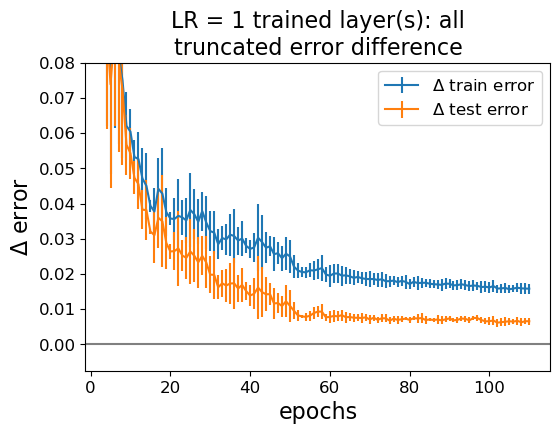
\includegraphics[width=5cm]{img/truncated_error/mlp3_trunc_error_by_epochs_LR_0_all_xmin.png}
        \label{fig:mlp3-trunc_err_epochs_xmin_1}
    }
    \subfigure[$lr=2\times$]{
        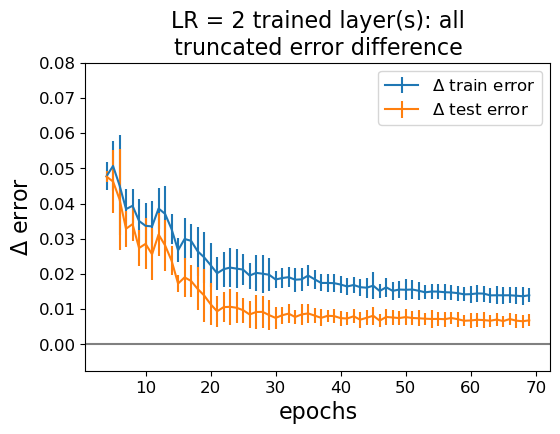
\includegraphics[width=5cm]{img/truncated_error/mlp3_trunc_error_by_epochs_LR_1_all_xmin.png}
        \label{fig:mlp3-trunc_err_epochs_xmin_2}
    }
    \subfigure[$lr=4\times$]{
        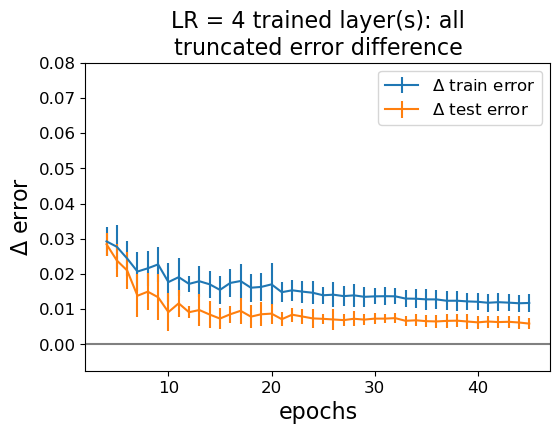
\includegraphics[width=5cm]{img/truncated_error/mlp3_trunc_error_by_epochs_LR_2_all_xmin.png}
        \label{fig:mlp3-trunc_err_epochs_xmin_4}
    }\\
    \subfigure[$lr=8\times$]{
        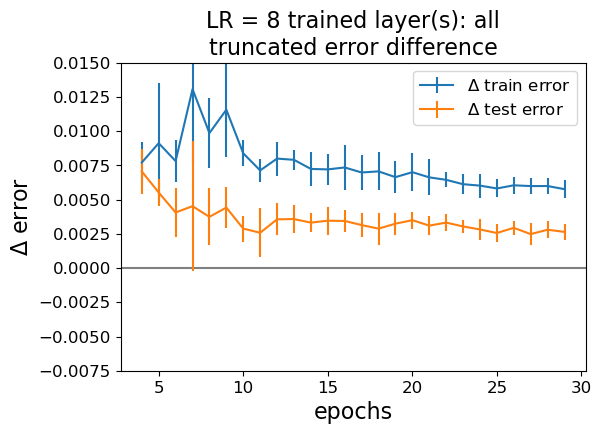
\includegraphics[width=5cm]{img/truncated_error/mlp3_trunc_error_by_epochs_LR_3_all_xmin.png}
        \label{fig:mlp3-trunc_err_epochs_xmin_8}
    }
    \subfigure[$lr=16\times$]{
        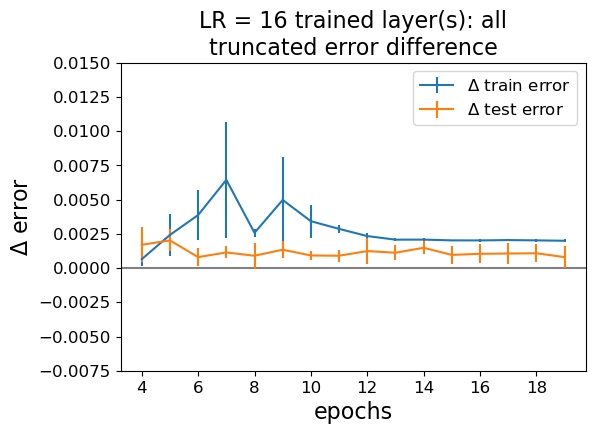
\includegraphics[width=5cm]{img/truncated_error/mlp3_trunc_error_by_epochs_LR_4_all_xmin.png}
        \label{fig:mlp3-trunc_err_epochs_xmin_16}
    }
    \subfigure[$lr=32\times$]{
        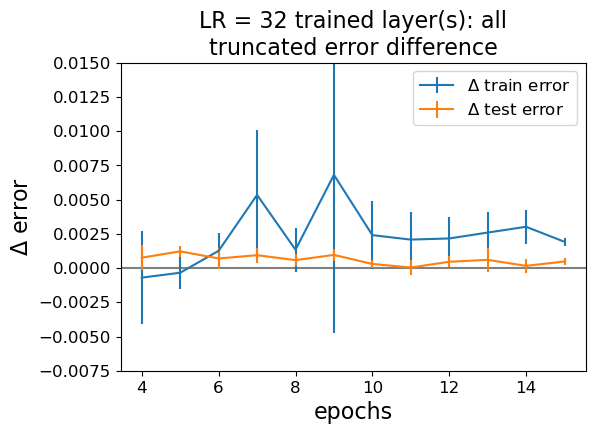
\includegraphics[width=5cm]{img/truncated_error/mlp3_trunc_error_by_epochs_LR_5_all_xmin.png}
        \label{fig:mlp3-trunc_err_epochs_xmin_32}
    }
    \caption{
            $\Delta E_{train}$ (blue) and $\Delta E_{test}$ (orange) for various learning rates, using the 
            \POWERLAW~MSR. As learning rate increases we can see that $\Delta E_{train}$ and $\Delta E_{test}$ both tend 
            towards lower asymptotic minima, which they reach after fewer epochs of training. We can also see that 
            (after the first few epochs,) $\Delta E_{train}$ (blue) is always higher than $\Delta E_{test}$ (orange). 
            Observe that in the bottom row (d--f) the yaxis is contracted to make the variation more visible. In (f) we can see 
            that as learning rate surpasses its optimal setting, the gap between $\Delta E_{train}$ and $\Delta 
            E_{test}$ begins to increase again, and has wider error bars, suggesting that the excessively large learning 
            rate is disrupting the MLP3s ability to lear the \EffectiveCorrelationSpace.
    }
    \label{fig:mlp3-msr-results-xmin}
    %Comparison of \POWERLAW~and \TRACELOG~ Model Selection Rules for testing the \EffectiveCorrelationSpace}
\end{figure}



To see how the \EffectiveCorrelationSpace forms, we plot how $\Delta E_{train}$ and $\Delta E_{test}$ evolve over training, for each of the various learning rates considered.%
\footnote{When batch size was varied, results did not significantly differ, and so they are omitted. 
%% CONFIRM WE HAVE SAID THIS ELSEWHERE %% See the experimental Colab notebooks for the full set of experiments.
} 

We start with the effect of the \POWERLAW~MSR.
See Figure~\ref{fig:mlp3-msr-results-xmin}, where we see that $\Delta E_{train}$ and $\Delta E_{test}$ generally trend 
downwards as they approach minimum train error. 
When the learning rate is larger, the models converge more quickly, and $\Delta E_{train}$ and $\Delta E_{test}$ also converge to lower values. 
Recall from Figure~\ref{fig:mlp3-accuracies-lr} that $lr=16\times$ had the lowest test error. In 
Figure~\ref{fig:mlp3-trunc_err_epochs_xmin_16}, we see that it also has the lowest $\Delta E_{train}$ and $\Delta 
E_{test}$. A lower $\Delta E_{train}$ or $\Delta E_{test}$ means that more of the models correct predictions are due to 
the low rank tail, meaning that the tail generalizes better, and we see here that when the tail generalizes best, the 
model was the most accurate. 

In each plot, we also see that the error bars are wide early on, before suddenly becoming much narrower. This transition 
is more visible in the larger learning rates shown in~\ref{fig:mlp3-trunc_err_epochs_xmin_8}--\ref{fig:mlp3-trunc_err_epochs_xmin_32},
but can also be seen in \ref{fig:mlp3-trunc_err_epochs_xmin_1}--\ref{fig:mlp3-trunc_err_epochs_xmin_4}, albeit less 
clearly. Most interestingly of all, this transition is preceded by a brief period, sometimes a single epoch, in which the 
error bars are drastically wider, in a way that is reminiscent of a first-order phase transition. Again, this 
phenomenon can be seen most clearly in ~\ref{fig:mlp3-trunc_err_epochs_xmin_8}--\ref{fig:mlp3-trunc_err_epochs_xmin_32}.


We next consider the effect of the \TRACELOG~MSR.
See Figure~\ref{fig:mlp3-msr-results-detX}, which also shows the development of $\Delta E_{train}$ and $\Delta E_{test}$ 
over epochs, where we see a very different pattern in the train error and test error. 
The difference in the train error is because, as the model is untrained in the early epochs, the \TRACELOG~MSR 
\emph{over}-estimates the tail by choosing a $\lambda_{min}$ that is too small. 
Thus, $\Delta E_{train}$ actually increases to its asymptotic value at the final epoch. 
In the earliest epochs, the truncated train error is even \emph{less} than the full MLP3 models error, suggesting that 
signal is forming in the large eigenvalues in these early epochs, but is swamped by the randomness of the early initial 
weights, some of which is then removed by truncation. As epochs progress, this effect disappears.
%
Here again we can see the ``phase-transition-like behavior of the train error, as the error bars are wide early on, up to a transition having an abnormally large error bar, after which they stabilize.

Perhaps most interestingly of all, we see that under the \TRACELOG Model Selection Rule (MSR), $\Delta E_{test}$ is flat \emph{throughout 
training}, and for all learning rates. This implies that there is \emph{no} point in training where the 
\TRACELOG tail generalizes badly. In other words, almost none of the out-of-sample variance falls outside of the \EffectiveCorrelationSpace, as the \TRACELOG~MSR over-estimates the \EffectiveCorrelationSpace. It also bears noticing that under the 
\POWERLAW~MSR, (Figure~\ref{fig:mlp3-msr-results-xmin},) this is decidedly not the case, because the \POWERLAW~MSR \emph{under}-estimates the \EffectiveCorrelationSpace. As we will see in \ref{sxn:empirical-trace_log}, as \ALPHA approaches $2$, the gap between the two MSRs goes to $0$.
%This means that a small, but 
%significant amount of generalization comes from the gap between these tails, but none at all %comes from the bulk.
%\nred{confusing}


\begin{figure}[t]
    \centering
    \subfigure[$lr=1\times$]{
        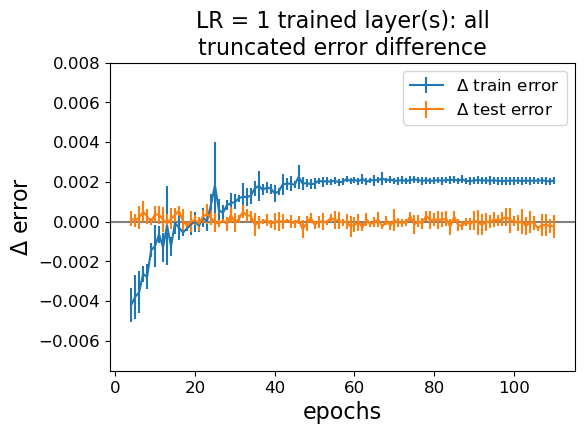
\includegraphics[width=5cm]{img/truncated_error/mlp3_trunc_error_by_epochs_LR_0_all_detX.png}
        \label{fig:mlp3-trunc_err_epochs_detX_1}
    }
    \subfigure[$lr=2\times$]{
        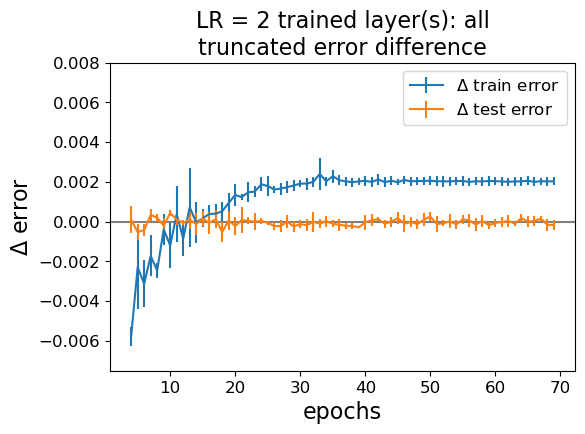
\includegraphics[width=5cm]{img/truncated_error/mlp3_trunc_error_by_epochs_LR_1_all_detX.png}
        \label{fig:mlp3-trunc_err_epochs_detX_2}
    }
    \subfigure[$lr=4\times$]{
        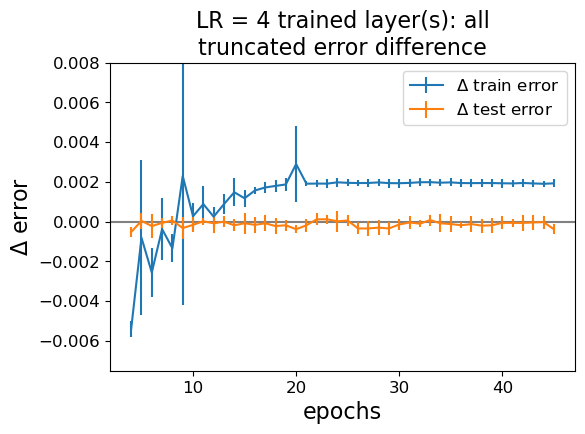
\includegraphics[width=5cm]{img/truncated_error/mlp3_trunc_error_by_epochs_LR_2_all_detX.png}
        \label{fig:mlp3-trunc_err_epochs_detX_4}
    }\\
    \subfigure[$lr=8\times$]{
        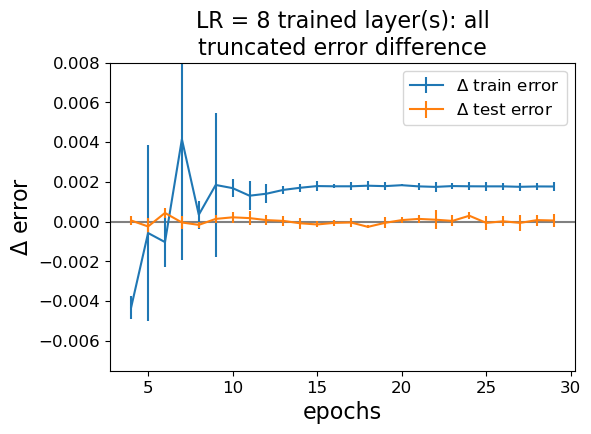
\includegraphics[width=5cm]{img/truncated_error/mlp3_trunc_error_by_epochs_LR_3_all_detX.png}
        \label{fig:mlp3-trunc_err_epochs_detX_8}
    }
    \subfigure[$lr=16\times$]{
        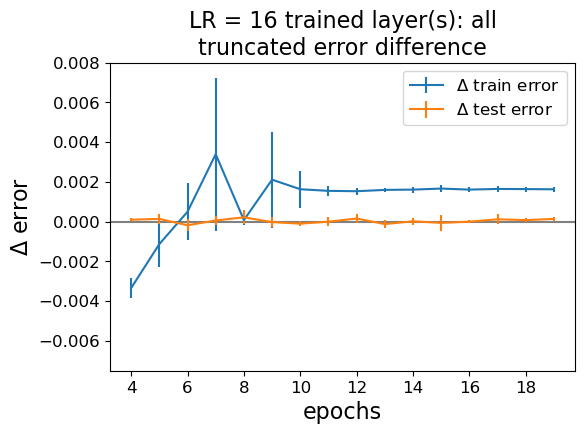
\includegraphics[width=5cm]{img/truncated_error/mlp3_trunc_error_by_epochs_LR_4_all_detX.png}
        \label{fig:mlp3-trunc_err_epochs_detX_16}
    }
    \subfigure[$lr=32\times$]{
        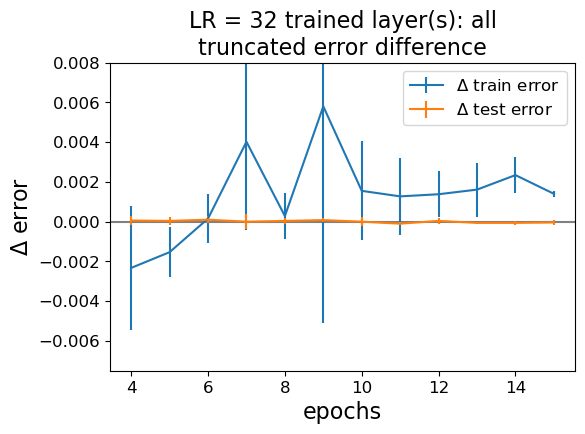
\includegraphics[width=5cm]{img/truncated_error/mlp3_trunc_error_by_epochs_LR_5_all_detX.png}
        \label{fig:mlp3-trunc_err_epochs_detX_32}
    }
    \caption{
        $\Delta E_{train}$ (blue) and $\Delta E_{test}$ (orange) for selected learning rates, using the \TRACELOG~MSR. 
        For all learning rates, $\Delta E_{test}$ is centered on $0$, meaning that the \TRACELOG~Effective Correlation 
        Space explains almost all variation in out-of-sample predictions, but it does \emph{not} explain all of the 
        training set predictions (blue). NOTE: The y axis is the same in all plots, and is much narrower than in 
        Figure~\ref{fig:mlp3-msr-results-xmin}. In (a--e) we can see that $\Delta E_{train}$ converges to approximately 
        $0.002$. Compare with Figure~\ref{fig:mlp3-trunc_err_epochs_xmin_16}, which reaches a minimum of approximately 
        $0.0025$. As in Figure~\ref{fig:mlp3-trunc_err_epochs_xmin_32}, the learning rate of $32\times$ normal disrputs the 
        MLP3s ability to discover the \TRACELOG \EffectiveCorrelationSpace.
    }
    \label{fig:mlp3-msr-results-detX}
    %Comparison of \POWERLAW~and \TRACELOG~ Model Selection Rules for testing the \EffectiveCorrelationSpace}
\end{figure}


There are two final points of comparison between Figures~\ref{fig:mlp3-msr-results-xmin} and~\ref{fig:mlp3-msr-results-detX}.
%
First, 
although it appears in Figure~\ref{fig:mlp3-msr-results-detX} that $\Delta E_{train}$ converges to a larger value than in Figure~\ref{fig:mlp3-msr-results-xmin}, this is because the scale of the y-axis is $10\times$ smaller. 
That is, the \POWERLAW~MSR is biased towards over-estimating $\lambda_{min}$, which means it over-truncates, producing a 
larger $\Delta E_{train}$ or $\Delta E_{test}$ 
than the \TRACELOG~MSR, which is biased towards under-estimating $\lambda_{min}$. 
%
Second,
in both Figure~\ref{fig:mlp3-msr-results-xmin} and~\ref{fig:mlp3-msr-results-detX}, we can see that $\Delta E_{test}$ is consistently lower than $\Delta E_{train}$. 
Clearly, truncating has a larger effect on train predictions, meaning that no matter how long the model is trained, some 
of the train predictions are still derived from the bulk. The fact that they remain is evidence that the gradient does not degrade them, meaning that they were most likely contributing spuriously correct answers. Yet, the test predictions are far less affected, meaning that only the \EffectiveCorrelationSpace contributes to the models ability to generalize.

\subsubsection{Truncation and Generalization}

%We can also estimate the test accuracies of the \emph{Truncated} models by evaluating the train accuracy of 
%\emph{Truncated} models
%\begin{align}
%  E_{test}\approx E^{\EFF}_{train}(\mathcal{D}) 
%\end{align}
%Generally speaking, this may not be as good of an approximation as above, but we
%can use this to study trends in the test accuracies for the \ALPHA and \ALPHAHAT metrics
%to see how \ALPHAHAT can correct for anamolously small alphas due to \CorrelationTraps.
Given that $\Delta E_{test}$ is always lower than $\Delta E_{train}$ for the \POWERLAW~MSR, and similarly for \TRACELOG~after a certain point in training, it is clear that the \EffectiveCorrelationSpace has something to do with generalization.
However, this leaves open the question of what role precisely \ALPHA plays. 
In Figure~\ref{fig:mlp3-alpha-generalization-gap}, we plot $\Delta E_{train}$ and $\Delta E_{test}$ with the \POWERLAW~MSR as a function of \ALPHA (rather than epochs) for layers FC1 and FC2, as well as the \GeneralizationGap -- that is, $E_{test} - E_{train}$. 
(Recall \EQN~\ref{eqn:gen_gap}.) 
Learning rate is not explicitly shown, but its effect can be seen in the clusters of points that each learning rate generates.

\begin{figure}[t]
  \centering
  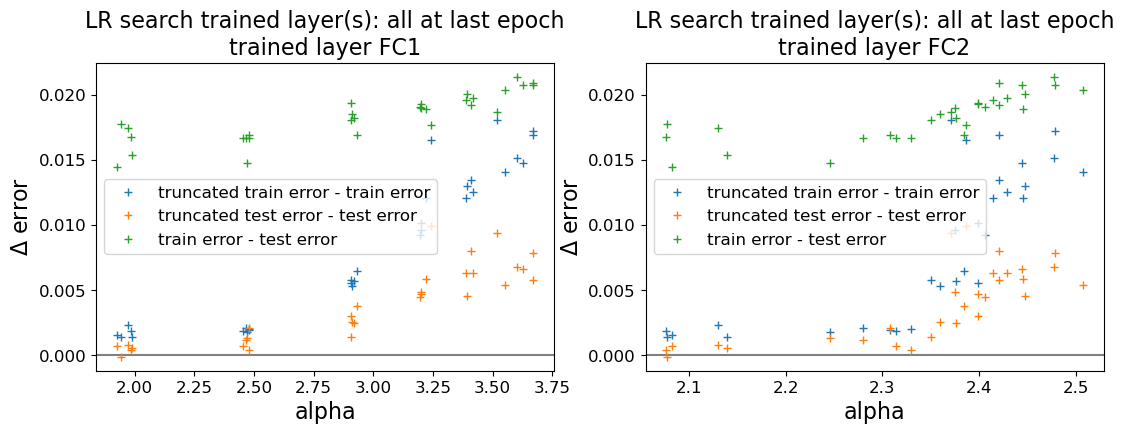
\includegraphics[width=15cm]{img/truncated_error/mlp3_trunc_error_by_LR_alpha_all_xmin.png}
  \caption{
        Train and test error gaps using the \POWERLAW~MSR, as a function of alpha in the FC1 and FC2 layers of MLP3 
        models, at the \emph{final epoch} of training. We can see that as alpha decreases towards $2$, (right to left), 
        $\Delta E_{train}$ and $\Delta E_{test}$ generally decrease as well, meaning that the closer $\ALPHA$ is to $2$, 
        the more the Effective Correllation Space explains the train and test predictions. The gap between un-truncated 
        train and test error, (\EQN \ref{eqn:gen_gap},) decreases as well until $\alpha_{FC1} < 2$.
  }
  \label{fig:mlp3-alpha-generalization-gap}
\end{figure}

In both layers, $\Delta E_{train}$ and $\Delta E_{test}$ steadily decrease with $\alpha_{FC1}$, until it passes below 
$2$, after which the relation deteriorates somewhat.
This is especially prominent in FC2. 
Recall from Figure~\ref{fig:mlp3-alphas-lr}, Section~\ref{sxn:empirical-test_acc}, that when $\alpha_{FC1}$ passed below $2$, the train error and test error both increased and exhibited larger variability. 
From this we interpret \ALPHA as a measure of \emph{regularization} (which is consistent with its introduction as a measure of 
implicit self-regularization~\cite{MM18_TR_JMLRversion}).
Regularization has the effect of keeping train and test accuracy closer together, and generally, as \ALPHA in the dominant layer decreases towards $2$ from above, the train-test error gap decreases.




\subsection{Evaluating the \TRACELOG  Condition}
\label{sxn:empirical-trace_log}

%Here, 
Having established that the PL tail of the ESD, defined by eigenvalues above $\LAMBDAPL$, is a major factor in determining model quality in the MLP3 model, we now examine how well the \TRACELOG  Condition compares with it. 
In particular, we demonstrate that when the tail of a layer ESD is described well by the \HTSR \Phenomenology, i.e., when 
it is well-fit by a PL with $\rho(\lambda)_{tail}\sim\lambda^{-\alpha}$, with PL exponent $\alpha\simeq2$, then the 
eigenvalues in the tail defined by the PL fit, i.e., $\lambda\ge\LAMBDAPL$, \emph{also} satisfy the \TRACELOG  Condition 
of \EQN~\ref{eqn:detX}---\emph{a key assumption of the \SETOL theory}.
This is a rather remarkable empirical result that couples \HTSR and \SETOL; it has its basis in our \SETOL derivation; and it provides the basis for an inductive principle that is based on the product of eigenvalues rather than an eigenvalue gap.

We can denote the eigenvalue that best fits the \TRACELOG  Condition as $\LAMBDADETX$. 
Then, to measure how well this condition holds, we can compute
\begin{align}
        \label{eqn:D_lambda_min}
        \Delta \lambda_{min} = \LAMBDAPL - \LAMBDADETX  .
\end{align}
In Sections~\ref{sxn:detx-mlp3} and~\ref{sxn:detx-sota}, we will see the trend that as $\alpha$ approaches $2$, $\LAMBDAPL$ and $\LAMBDADETX$ also approach one another, and hence $\Delta \lambda_{min}$ goes to $0$, from above, both for our toy MLP3 model as for SOTA models.
In our MLP3 model, we will see that a crossing of the equality condition coincides with over-regularization and a degradation in model accuracy. 
In pre-trained ResNet\cite{ResNet15_TR}, VGG\cite{VGG14_TR} and ViT\cite{VIT20_TR} models, we will also see, empirically, that in general $\Delta \lambda_{min}$ remains positive, just as $\alpha$ remains above $2$.


\subsubsection{The MLP3 model}
\label{sxn:detx-mlp3}

Consider Figure~\ref{fig:mlp3-tracelognorm}, which shows $\LAMBDAPL$ and $\LAMBDADETX$ in the FC1 layer of three MLP3 models, each sharing a common starting random seed, that were trained with the largest learning rates.
The $\LAMBDAPL$ and $\LAMBDADETX$ eigenvalues are marked by red and purple vertical lines, respectively; and thus $\Delta \lambda_{min}$ is the distance between red and purple lines.
%
As learning rate increases, the red and purple lines draw closer, and they are closest for $lr=32\times$ (Figure~\ref{fig:mlp3-randesd-32}). 
(Compare this with Figure~\ref{fig:mlp3-alphas-lr}, Section~\ref{sxn:empirical-test_acc}, which shows that this corresponds with an increase in test accuracy, up to $lr=16\times$, but at $lr=32\times$ \ALPHA fell below $2$ and accuracy suffered.) 
In Figure~\ref{fig:mlp3-randesd-8}-\ref{fig:mlp3-randesd-16}, the purple line is left of the red line; but in Figure~\ref{fig:mlp3-randesd-32}, the red and purple lines cross, such that $\LAMBDAPL < \LAMBDADETX$.
This is analogous to the case where $\alpha$ crosses below $2$. 
This suggests that the absolute \TRACELOG  is minimized when $\alpha\simeq2$, which (remarkably) is exactly when the \HTSR \Phenomenology predicts the layer is \Ideal.

(Observe that \Ideal does not necessarily mean optimal under a finite sized training set, but rather that the finite-sized system behaves the most similarly to its infinite limit.)

\begin{figure}[t] %[h]
    \centering
    \subfigure[$LR=8\times$]{
      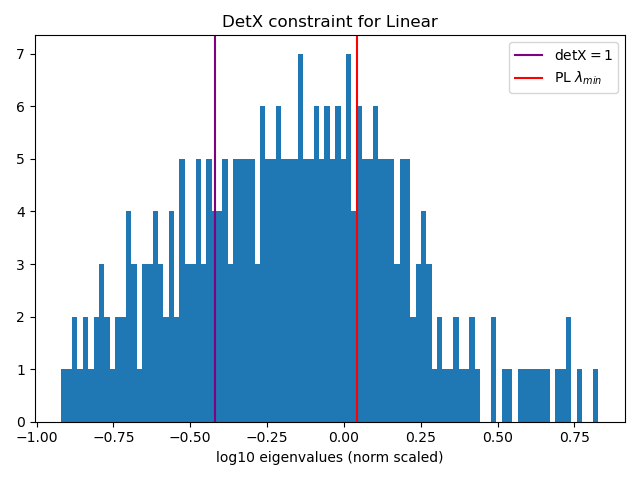
\includegraphics[width=5cm]{./img/detX_plots/LR=8/FC1/ww.layer3.detX.png}
        \label{fig:mlp3-randesd-8}
    }
    \subfigure[$LR=16\times$]{
      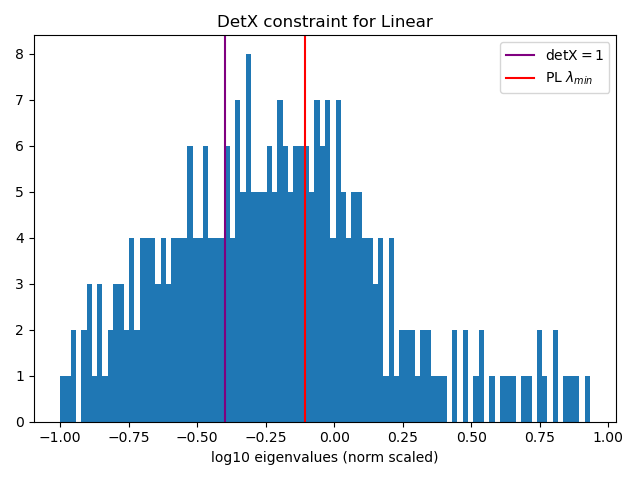
\includegraphics[width=5cm]{./img/detX_plots/LR=16/FC1/ww.layer3.detX.png}
        \label{fig:mlp3-randesd-16}
    }
    \subfigure[$LR=32\times$]{
      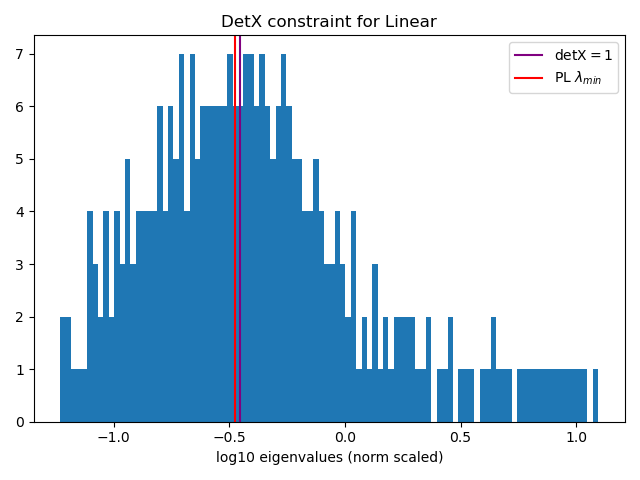
\includegraphics[width=5cm]{./img/detX_plots/LR=32/FC1/ww.layer3.detX.png}
        \label{fig:mlp3-randesd-32}
    }
    \caption{
        Log-Linear ESDs for three learning rates in the FC1 layer of MLP3. The red line shows $\LAMBDAPL$, and the 
        purple line shows $\LAMBDADETX$. Observe that the purple line is to the left of the red line, but as the LR 
        increases they move closer together. However, when LR is $32\times$, where both 
        train and test accuracy suffered (c), the red line is to the left of the purple line. This is often a signature 
        of an \OverRegularized layer, and indeed the FC1 layer in this model had $\alpha < 2$. (See Figure~\ref{fig:mlp3-alpha-fc1-by-lr} in 
        Section~\ref{sxn:empirical-test_acc}.)
    }
    \label{fig:mlp3-tracelognorm}
\end{figure}


We can compare  $\alpha$ and $\Delta \lambda_{min}$ more broadly by plotting $\Delta \lambda_{min}$ directly as a function of $\alpha$ in a single plot spanning all random seeds and learning rates or batch sizes.
This is shown in Figure~\ref{fig:mlp3-detx-gap}. 
Critical values of $\alpha=2$ and $\Delta \lambda_{min} = 0$ are shown as vertical and horizontal red lines, respectively. 
Values for various learning rates are plotted for layer FC1 
(Figure~\ref{fig:mlp3-detx-lr_search_fc1}) and FC2 (Figure~\ref{fig:mlp3-detx-lr_search_fc2}), as well as for various batch sizes in layer FC1 (Figure~\ref{fig:mlp3-detx-bs_search_fc1}) and FC2 (Figure~\ref{fig:mlp3-detx-bs_search_fc2}).

For layer FC1 (Figures~\ref{fig:mlp3-detx-lr_search_fc1} and~\ref{fig:mlp3-detx-bs_search_fc1}), in both cases we see near-linear march towards the critical tuple of $(\alpha, \Delta\lambda_{min}) = (2, 0)$.
In addition, passing this critical value coincides with diminished train and test accuracy, (recall 
Figure~\ref{fig:mlp3-accuracies}), suggesting that just as $\alpha=2$ is a threshold of over-regularization, $\LAMBDAPL < \LAMBDADETX$ may be as well. 
Since FC1 is the dominant layer, comprising roughly $8/9$ of the weights of the model, (Table~\ref{tab:mlp3},) we expect 
FC1 to most closely match the performance of the model as a whole.

For layer FC2, which comprises roughly the other $1/9$ of the models weights, there is a similar coevolution, but it is weaker. 
As learning rate or batch size exceeds their critical values, rather than going to $(2, 0)$ as in FC1, we instead see that the relationship simply breaks down, with the gap growing larger even as $\alpha$ decreases. 
Given that FC1 \emph{has} passed the critical $\alpha=2$ threshold, we conjecture that the breakdown of the relationship between $\alpha$ and $\Delta \lambda_{min}$ is due to FC1 becoming \ATypical.


\begin{figure}[t] %[h]
    \centering
    \subfigure[Layer FC1 for various learning rates]{
        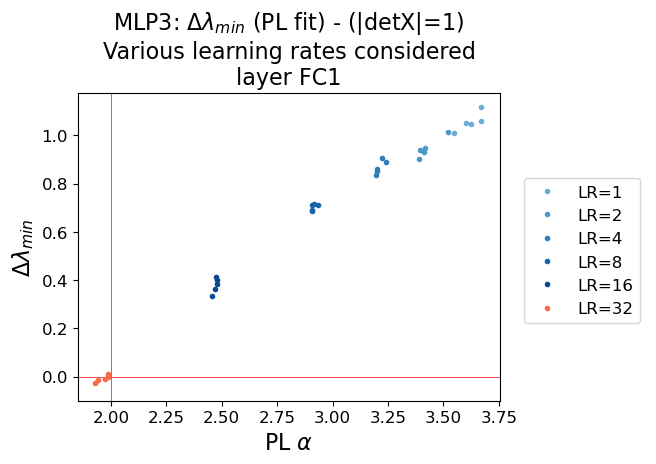
\includegraphics[width=7cm]{img/detX_plots/mlp3_detX_delta_LR_all_FC1.png}
        \label{fig:mlp3-detx-lr_search_fc1}
    }
    \subfigure[Layer FC2 for various learning rates]{
        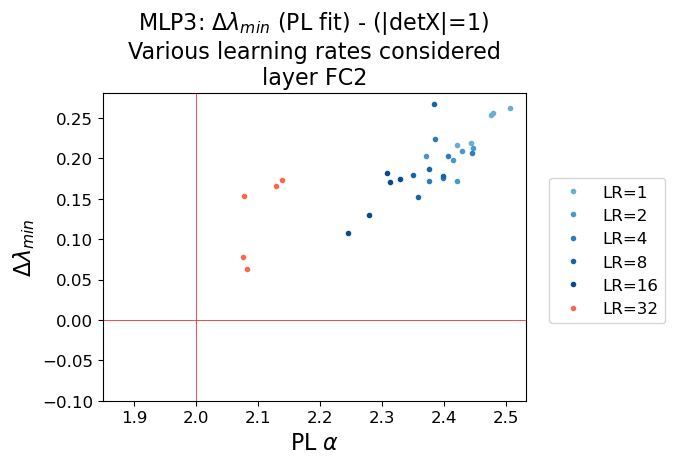
\includegraphics[width=7cm]{img/detX_plots/mlp3_detX_delta_LR_all_FC2.png}
        \label{fig:mlp3-detx-lr_search_fc2}
    }\\
    \subfigure[Layer FC1 for various batch sizes]{
        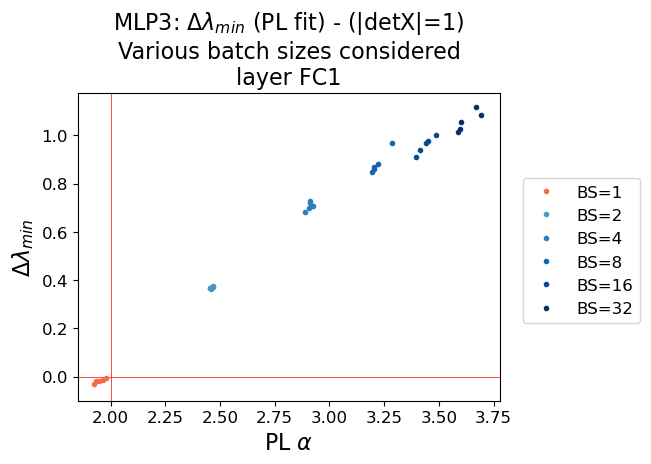
\includegraphics[width=7cm]{img/detX_plots/mlp3_detX_delta_BS_all_FC1.png}
        \label{fig:mlp3-detx-bs_search_fc1}
    }
    \subfigure[Layer FC2 for various batch sizes]{
        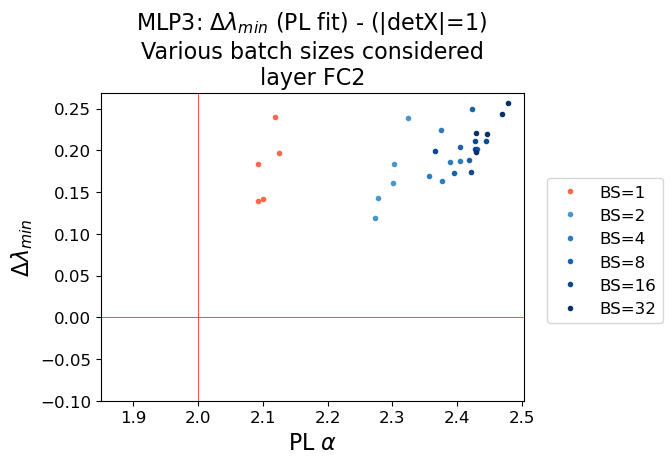
\includegraphics[width=7cm]{img/detX_plots/mlp3_detX_delta_BS_all_FC2.png}
        \label{fig:mlp3-detx-bs_search_fc2}
    }
    \caption{
            MLP3 Model: Comparison of the PL \ALPHA (x-axis), with the difference between $\LAMBDAPL$ and $\LAMBDADETX$ 
            (y-axis). The thin red lines indicate critical values of $\alpha=2$ and $\Delta \lambda_{min} = 0$. As 
            learning rate increases (a--b) or batch size decreases (c--d), we can see that in layer FC1, which dominates 
            the model, (See Table~\ref{tab:mlp3},) $\alpha$ goes to $2$, and $\Delta \lambda_{min}$ goes to $0$. Observe 
            that both critical values are crossed at the most extreme hyper-parameter selection, (red,) corresponding 
            with over-training. Layer FC2 shows a weaker tendency towards the critical values (b, d), and is disrupted 
            at the most extreme hyper-parameter values (red).
    }
 \label{fig:mlp3-detx-gap}
\end{figure}


\subsubsection{State-of-the-Art (SOTA) models}
\label{sxn:detx-sota}

Here, we consider SOTA models, 
in particular VGG pre-trained models~\cite{VGG14_TR}, the ResNet series~\cite{ResNet15_TR}, the ViT 
series~\cite{VIT20_TR}, and the DenseNet series~\cite{DenseNet17_TR}.
We show that as $\alpha$ approaches $2$, the Log-Trace Condition holds better and better, i.e., $\Delta\lambda_{min}$ 
approaches $0$.
%holds approximately for the PL portion of the tail
%even when $\alpha\gg2$ in some cases.

\begin{figure}[t] %[h]
    \centering
    \subfigure[VGG Series]{
      \includegraphics[width=7cm]{./img/VggTest.png}
      \label{fig:VGG_trend}
    }
    \subfigure[ResNet Series]{
      \includegraphics[width=7cm]{./img/ResNetTest.png}
      \label{fig:ResNet_trend}
    } \\
    \subfigure[ViT Series]{
      \includegraphics[width=7cm]{./img/VIT_ESD_trends.png}
      \label{fig:VIT_trend}
    }
    \subfigure[DenseNet Series]{
      \includegraphics[width=7cm]{./img/DenseNetTest.png}
      \label{fig:DenseNet_trend}
    }
    \caption{Difference between the two $\lambda_{min}$ estimates, $\Delta\lambda_{min}$, (\EQN~\ref{eqn:D_lambda_min}), as a 
        function or $\alpha$, for linear and convolutional layers in series of VGG~\cite{VGG14_TR}, ResNet~ 
        \cite{ResNet15_TR}, ViT models~\cite{VIT20_TR} and DenseNet models~\cite{DenseNet17_TR}. Layer matrices for all 
        models in the series were pooled to create each plot. In (a), (VGG,) we see three clusters of points -- those 
        with $\Delta \lambda_{min}$ close to $0$ and $\alpha$ close to $2$, those with $\Delta \lambda_{min}$ above $2$ 
        and $\alpha > 2.5$, and those with $\Delta \lambda_{min}$ above $6$ and $\alpha > 3.5$. In (b), (ResNet,) we see 
        that in general, as $\alpha$ shrinks towards $2$, $\Delta \lambda_{min}$ tends towards $0$, overshooting 
        slightly. We also see that the difference $\Delta\lambda_{min}$ is almost always positive, with few exceptions, 
        and even the layers that do not overshoot form a kind of ``funnel shape pointing towards the critical point 
        $(2, 0)$. In (c), (ViT,) we also see the same general relationship between $\alpha$ and $\Delta \lambda_{min}$ 
        across layers of several ViT models. Observe that ViT models do not have convolutional layers, and in spite of 
        this, the overall pattern is similar. In (d), (DenseNet,) we see a similar overall trend as in (b), except that 
        $\Delta\lambda_{min}$ tends to decrease sooner, but there are also more layers with $\alpha < 2$ and 
        $\Delta\lambda_{min}$ above $0$.
    }
  \label{fig:CV_ESD_trends}
\end{figure}


Figure~\ref{fig:CV_ESD_trends} plots $\alpha$ versus the difference $\Delta\lambda_{min}$, (\EQN~\ref{eqn:D_lambda_min}).
Layer matrices from all models in each series are pooled to generate the plots.% 
\footnote{For convolutional layers, the \WW tool first computes eigenvalues for all channels-to-channels linear operators separately, and then pools them in order to compute $\alpha$, $\LAMBDAPL$ and $\LAMBDADETX$. For instance, in a $64\times 64\times 3\times 3$ weight tensor, there would be $9$ separate linear operators of $64\times 64$, giving $576$ eigenvalues, which would then be pooled to compute $\alpha$, $\LAMBDAPL$ and $\LAMBDADETX$.} 
Notice that in Figure~\ref{fig:VGG_trend} -- \ref{fig:DenseNet_trend}, $\Delta\lambda_{min}$ approaches zero as $\alpha\rightarrow 2$ from above. 
Individual points may have a large $\Delta\lambda_{min}$ for an $\alpha$ near to $2$, but the overall trend is apparent. 
The rapid decrease of $\Delta\lambda_{min}$ as $\alpha$ approaches $2$ from above implies that the PL tail rapidly 
takes on a unit \TRACELOG  (if it doesn't already have it.)

As we saw in comparison of Figures~\ref{fig:mlp3-msr-results-xmin} and~\ref{fig:mlp3-msr-results-detX}, 
(Section~\ref{sxn:trunc_err_epochs},) the \TRACELOG tail is generally larger, and always has highly generalizing 
components. Thus, it is plausible that as layers reach the limit of the amount of information that can be encoded in 
them, i.e. as $\alpha$ goes to $2$, the \POWERLAW~tail expands to fill the \TRACELOG tail. This effect can be seen 
clearly in Figure~\ref{fig:CV_ESD_trends} in the condensing of the ``funnel shape.

Recall from Figure~\ref{fig:mlp3-detx-gap} that layer FC1 dominated the model, (Table~\ref{tab:mlp3},) producing a clear 
progression of $\alpha$ and $\Delta\lambda_{min}$ towards $(2, 0)$, as a function of learning rate or batch size, whereas FC2 showed a slightly less clear relationship. 
In larger models having dozens or hundreds of layers, we would not expect any one layer to dominate as thoroughly.
Moreover, it is the architecture that varies between models in each series, not (necessarily) the hyperparameters, meaning that there would not be a straight line, as in Figures~\ref{fig:mlp3-detx-lr_search_fc1} and~\ref{fig:mlp3-detx-bs_search_fc1}. 
However, with all of the layers contributing to varying degrees, we nevertheless see a clear trend in all plots of Figure~\ref{fig:CV_ESD_trends}. 
These results show how the single-layer \SETOL theory extends from the MLP3 model, which is dominated by a single layer, to larger models where many layers interact in complex ways, but still reflect the same overall trend.


\begin{figure}[t] %[h]
    \centering
    \subfigure[Falcon 7B]{
      \includegraphics[width=7cm]{./img/FALCON7b_ESD_trends.png}
      \label{fig:falcon7B_trend}
    }
    \subfigure[Falcon 40B]{
      \includegraphics[width=7cm]{./img/FALCON40b_ESD_trends.png}
      \label{fig:falcon40B_trend}
    }
    \subfigure[Llama 13B]{
      \includegraphics[width=7cm]{./img/LLAMA_13b_ESD_trends.png}
      \label{fig:llama13B_trend}
    }
    \subfigure[Llama 65B]{
      \includegraphics[width=7cm]{./img/LLAMA_65b_ESD_trends.png}
      \label{fig:llama65B_trend}
    }
    \caption{Difference between the two $\lambda_{min}$ estimates, $\Delta\lambda_{min} = \LAMBDAPL - \LAMBDADETX$, 
        as a function of $\alpha$, for all linear layers in the FALCON\cite{falcon40b}(a-b) and 
        LLAMA \cite{touvron2023_TR}(c-d) language models for varying numbers of parameters. As in Figure 
        \ref{fig:CV_ESD_trends}, we see that in recent Large Language Models, $\Delta\lambda_{min}$ remains positive, 
        except where $\alpha < 2$ (d). Otherwise, a ``funnel shape can still be seen leading towards the critical 
        point $(2, 0)$ as in Figures~\ref{fig:ResNet_trend} and~\ref{fig:VIT_trend} Observe that the x- and y-axes are 
        different between sub-figures due to the differences in scale of each model.
    }
  \label{fig:LLM_ESD_trends}
\end{figure}

The overall pattern of relationship between $\Delta\lambda_{min}$ and $\alpha$ can also be seen in 
Figure~\ref{fig:LLM_ESD_trends}, which shows plots for Large Language Models (LLMs) of the Falcon~\cite{falcon40b} and 
LLAMA~\cite{touvron2023_TR} model families, for different numbers of parameters. Observe that each 
subfigure~\ref{fig:falcon7B_trend}--\ref{fig:llama65B_trend} shows a single 
model, rather than a collection of models in a family, as in Figure~\ref{fig:CV_ESD_trends}.
The y-axis is the same between models in the same family. 
As in Figure~\ref{fig:CV_ESD_trends}, there is a general outline of a ``funnel shape pointing towards the critical 
point $(2, 0)$, with the exception that it is only reached in the case of LLAMA-65b, (Figure~\ref{fig:llama65B_trend}). 
This suggests that these LLMs are larger than they necessarily need to be, consistent with prior work~\cite{YHTx21_TR}, 
but also that they are well guarded against \OverRegularized layers beyond the critical point
($\alpha=2$ and $\Delta\lambda_{min}=0$).



\subsection{Model Quality: Computational \RTransforms}
\label{sxn:empirical_comp_r_transforms}

In this Section, we look at how the \HTSR layer quality HT PL metric $\alpha$
compares to computing the \LayerQualitySquared $\QT$ using
the Computational \RTransform method proposed in Section~\ref{sxn:comp_rmt}
for fully trained MLP3 model(s).
Figure~\ref{fig:MLP3_qualities}
presents results for FC1 and FC2 layers, comparing
both the batch size and the mean $\alpha$ metric to the
mean $\QT$, and the results are quite different.


\begin{figure}[t]
    \centering
    \subfigure[FC1 batch size vs $\QT$]{
        \includegraphics[width=6cm]{img/FC1_bs_vs_Q.png}
        \label{fig:FC1_bs_vs_Q}
    }
    \hspace{1cm} % Add space between subfigures
    \subfigure[FC1 Layer $\alpha$ vs $\QT$]{
        \includegraphics[width=6cm]{img/FC1_alpha_vs_Q.png}
        \label{fig:FC1_alpha_vs_Q}
    }
    \hspace{1cm} % Add space between subfigures
    \subfigure[FC2 batch size vs $\QT$]{
        \includegraphics[width=6cm]{img/FC2_bs_vs_Q.png}
        \label{fig:FC2_bs_vs_Q}
    }
    \hspace{1cm} % Add space between subfigures
    \subfigure[FC2 Layer $\alpha$ vs $\QT$]{
        \includegraphics[width=6cm]{img/FC2_alpha_vs_Q.png}
        \label{fig:FC2_alpha_vs_Q}
    }
    \caption{
      Evaluation of the computational \RTransform \LayerQualitySquared metric $\QT$
      on the fully trained MLP3 model(s) for different batch sizes.
    }
    \label{fig:MLP3_qualities}
\end{figure}


For FC1, as shown in Figure~\ref{fig:FC1_bs_vs_Q}, the quality metric \(\QT\) increases as the batch size decreases, following the expected trend. Notably, for batch size = 1, the quality metric exceeds $100\%$,
which suggests that the layer may be overfit in this scenario, which is similar to results obtained earlier. Furthermore, in Figure~\ref{fig:FC1_alpha_vs_Q}, the quality metric \(\QT\) shows a strong correlation with the $\alpha$ metric, consistent with the theoretical predictions of the \HTSR framework.
Earlier results suggest that the FC1 layer captures most of the correlation in the data,
so it is interesting that this layer also has much smaller error bars, indicating more consistent computational
quality across different batch sizes.

In contrast, for FC2, while the general trends are similar (as shown in Figures~\ref{fig:FC2_bs_vs_Q} and~\ref{fig:FC2_alpha_vs_Q}), the error bars on the quality metric $\QT$ are much larger. This indicates significantly higher variability in computational quality compared to FC1. The large error bars for FC2 suggest that, while the $\QT$ metric is theoretically grounded, it is less effective than the existing \HTSR layer quality metric $\alpha$, which exhibits greater stability and reliability in capturing layer behavior. These differences highlight the distinct computational characteristics of the two layers, with FC1 demonstrating more predictable trends that align closely with theoretical expectations.




\subsection{Inducing a Correlation Trap}
\label{sxn:empirical-correlation_trap}

\begin{figure}[t]
    \centering
    \subfigure[MLP3 \LearningRate $16\times$]{
%        \includegraphics[width=6cm]{img/log-esd-bs2.png}
        \includegraphics[width=6cm]{img/correlation_traps/LR_16_FC1_0/ww.layer3.randesd2.png}
        \label{fig:mlp3-accuracies3_lr16_trap}
    }
    \subfigure[MLP3 \LearningRate $32\times$]{
        \includegraphics[width=6cm]{img/correlation_traps/LR_32_FC1_0/ww.layer3.randesd2.png}
        \label{fig:mlp3-accuracies3_lr32_trap}
    }
    \caption{ESD plots for learning rate $lr=16\times$ and $lr=32\times$ normal, shown on Log-Lin scale, as computed 
    using the \WW tool, for the FC1 weight matrix $\mathbf{W}$ (green) and an element-wise randomized $\mbox{rand}(\mathbf{W})$ (red).  
    This provides an example of inducing a \CorrelationTrap in the MLP3 model, simply by increasing the learning rate used during model training.  
        See Section~\ref{sxn:Traps}.
            }
    \label{fig:mlp3-accuracies3}
\end{figure}


Previous work on the \HTSR \Phenomenology \cite{MM20a_trends_NatComm,MM21a_simpsons_TR} has shown that one can look for 
quantitative deviations from the necessary pre-conditions of tradtitional \RMT (particularly that the weights are 
$0$-mean and finite variance) to detect when a model layer suffers from some other anomaly in the elements, which we 
call a ``\CorrelationTrap (see Section~\ref{sxn:Traps} and ~\cite{MM20a_trends_NatComm,MM21a_simpsons_TR}). A 
\CorrelationTrap may cause, or be caused by, the over-regularization leading \ALPHA to fall below $2$, (see 
Section~\ref{sxn:underfitting}). Here, we explore this in greater detail, in light of our \SETOL.

% Recall that a \CorrelationTrap arises when the randomized spectrum 
% is not an MP distribution. In this case, we know contrapositively that one or more of the MPs conditions on the 
% element-wise distribution ($0$-mean and finite variance) are not met. When the MP laws conditions are not met, we do 
% not have the usual guarantee that the element-wise distribution alone \emph{cannot} produce a large eigenvalue, meaning 
% that some of the large eigenvalues are likely not a result of correlations between pairs of data elements. 
%
Lets look at the ESDs of the FC1 layer of the MLP3 model, for learning rates $lr=16\times$ and $lr=32\times$ normal. 
We will be interested in the general shape of the ESD of $\tfrac{1}{N}\mathbf{W}^T\mathbf{W}$.
For the purposes of detecting a \CorrelationTrap, we will randomize $\mathbf{W}^T\mathbf{W}$ element-wise, and then observe its largest eigenvalue $\lambda^{max}_{rand}$. 
%%Randomizing element-wise is a way of drawing a sample random matrix whose elements are i.i.d.  from the same distribution as $\mathbf{W}^T\mathbf{W}$, so that any violations of the MP laws preconditions can be seen. 

Figure~\ref{fig:mlp3-accuracies3} shows the ESDs of the original matrix (green) and the element-wise 
randomized $\mbox{rand}(\tfrac{1}{N}\mathbf{W}^T\mathbf{W})$ (red). 
Observe in particular $\lambda^{max}_{rand}$ for each learning rate factor.
For $lr=16\times$, Figure~\ref{fig:mlp3-accuracies3_lr16_trap} shows 
that the ESD of $\tfrac{1}{N}\mathbf{W}^T\mathbf{W}$ is HT, whereas the ESD of the randomized matrix is essentially a distorted semi-circle---as expected from the well-known MP result; and 
that $\lambda^{max}_{rand}$ lies at the edge of the random \MPBulk ESD.
(A similar result is seen for smaller learning rates.)  
In contrast, for $lr=32\times$, Figure~\ref{fig:mlp3-accuracies3_lr32_trap} shows 
that while the original ESD is again HT, the ESD of the randomized has one large element, $\lambda^{max}_{rand}$, that pulls out from the MP bulk.
%
This is the signature of a \CorrelationTrap; and it co-occurrs with the exact learning rate setting that degraded the train and test accuracies, pushing \ALPHA below its optimal value of $\alpha\simeq 2$.
%
When this happens,  both the estimation of \ALPHA and the formation of a PL tail are potentially disrupted. 
%
%%Thus, by increasing the learning rate to $lr=32\times$ normal, we were able to systematically induce a \CorrelationTrap, 

\CorrelationTraps have been observed previously~\cite{MM20a_trends_NatComm,MM21a_simpsons_TR}, using the \HTSR \Phenomenology.
However, \SETOL provides an explanation for why this would be expected to occur --- non-standard element-wise distributions will tend to interfere with the properties of the spectrum which \SETOL analyzes. 
Our derivation in Section~\ref{sxn:empirical} suggests that in order to apply the \SETOL effectively one must avoid (or remove) such traps. 
This too has been observed previously~\cite{MM20a_trends_NatComm,MM21a_simpsons_TR}. 


%\chris{There was some old discussion on alphahat that I have commented here.}
%Notice that, in Figure~\ref{fig:mlp3-accuracies2_mlp3-alphahat},
%and in contrast to \ALPHA, however, the \ALPHAHAT value for $bs=1$ is larger, not smaller,
%and almost follows the trend the other values show.   This happens because
%the \ALPHAHAT metric corrects for the anomalous \Scale in the $bs=1$ case.
%Since $\ALPHAHATEQN=\alpha\log_{10}\lambda_{max}$, the metric multiplies the spuriously
%small $\alpha$ by the spuriously large $\log_{10}\lambda_{max}$, and there
%is a fortuitous cancellation of errors.  This is, in part, why the (layer averaged)
%\ALPHAHAT can describe trends in the quality of models when using just \ALPHA fails.




\subsection{Overloading and the Hysteresis Effect}
\label{sxn:hysteresis_effect}

%Here, we do such-and-such. 
%XXX.  HOW PRECISELY TO FRAME.

\michaeladdressed{This par should go somewhere.  Where?}
\charles{@michael: again, no changes to section 6}
Obtaining a value of $\alpha$ outside the $\alpha \gtrsim 2$ range is indicative of ``overloading~\cite{SST92} that layer. 
This can be accomplished, e.g., by training only one layer in the MLP3 model.
As the two layers have very different sizes, we see markedly different behaviors, that are nevertheless consistent with theory.

The \SETOL theory is based on the idea that NNs undergoing training behave like Statistical Mechanic systems relaxing to an equilibrium. 
So far, we have tested the theory under conditions that are approaching \Ideal. 
However, for the theory to be useful in practice, we must also examine how it performs in non-\Ideal situations. 
Of particular interest, we would like to examine the theory under conditions where the training dynamics slows down, i.e., when it is in a ``glassy''
or meta-stable state. 
One way we can do this is to train only one layer, and freeze the rest. 
Doing so overloads the single trainable weight matrix, as a function of the ratio of examples to trainable
parameters~\cite{SST92,Gardner_1988,MM17_TR}, and we expect this to cause $\alpha_{FC1}$ or $\alpha_{FC2}$ to drop well below $2$. As in \ref{sxn:empirical-effective_corr_space}, we will be examining this effect over the entire course of training.

\michaeladdressed{@chris: reorganize the figures in this section, like we discussed.  Also, organie the text properly into each subsubsection.}
\chris{Ive split the figures and re-organized. Lets discuss.}

\subsubsection{Baseline: Loading onto both FC1 and FC2}
\label{sxn:hysteresis_baseline}
\begin{figure}[t] %[h]
    \centering
%    \subfigure[FC1 \ALPHA vs train and test error]{
        \includegraphics[width=15cm]{img/alpha_by_scales/mlp3_error_by_LR_all_FC1_binned.png} \\
%        \label{fig:mlp3-FC1-alpha-all-trained}
%    }\\
    \begin{tabular}{ccc}
      (a)\hspace{5cm} & (b) 
    \end{tabular}
%    \subfigure[FC2 \ALPHA vs train and test error]{
        \includegraphics[width=15cm]{img/alpha_by_scales/mlp3_error_by_LR_all_FC2_binned.png}
%        \label{fig:mlp3-hyst-all-FC2-LR32}
%    }
    \begin{tabular}{ccc}
      (c)\hspace{5cm} & (d) \\
    \end{tabular}
    \caption{
        Train (a, c) and test (b, d) accuracy as a function of $\alpha_{FC1}$ (a, b) and $\alpha_{FC2}$ (c, d) when {\bf all 
        layers are trained}. Red vertical lines show the critical value of $\alpha = 2$, and dashed black lines show 
        linear fits of error, using only points where $\alpha > 2$ and train error $> 0.001$. 
        For FC1 (a, b), we can see that each learning rate 
        produces a different trajectory of train error (a) and test error (b) as a function of $\alpha_{FC1}$, 
        showing that even though FC1 dominates overall, (Table~\ref{tab:mlp3},) FC2 still plays a modulating role. 
        (Cf. Figure~\ref{fig:mlp3-FC1-alpha-overloaded} where there is only one trajectory.)
        In (c, d) we can see that $\alpha_{FC2}$ never goes below $2$. As in (a, b), each learning rate 
        produces a different trajectory, though there is greater overlap for lower learning rates. See discussion in 
        Section~\ref{sxn:hysteresis_baseline}.
    }
    \label{fig:mlp3-baseline-load}
\end{figure}


%\michaeladdressed{Backpoint explicitly to what figs/section is being referred to here.} Done

To start, Figure~\ref{fig:mlp3-baseline-load} shows $\alpha_{FC1}$ and $\alpha_{FC2}$, binned in units of $0.05$, versus 
train and test error over all epochs of training
\footnote{Excluding the first four epochs when the matrix is still essentially random.} 
for each of the different learning rates considered. 
(Cf. Figures~\ref{fig:mlp3-alphas-lr} and~\ref{fig:mlp3-alphas-bs}, Section~\ref{sxn:empirical-effective_corr_space},
which show only the final epoch.)
Binning was done so as to facilitate averaging over the $5$ starting random seeds; 
linear fits are shown separately for each learning rate; and
error bars represent one standard deviation within each bin. 
The critical value of $\alpha=2$ is shown as a vertical red line in all plots. 
For each learning rate, train error and $\alpha$ decrease together during training, which can be seen for both 
$\alpha_{FC1}$ (a) and $\alpha_{FC2}$ (c), reading each line from the top right to bottom left. Test errors, (b, d) show 
a similar trend, but with wider error bars. 
Observe that the range of the y-axis is narrower for test error to make detail more visible.
\chris{CH TODO: Double check these plots. The y-axis should be the same vertically.}

We see in Figure~\ref{fig:mlp3-baseline-load} (a,b) 
\michaeladdressed{soft-code, dont hard-code subfigure references}
\chris{Splitting these figures is manual, so the soft-coding is a stand-in until they are finalized and frozen.}
that the $32\times$ learning rate causes $\alpha_{FC1}$ to decrease faster than any other, putting it on course to 
fall below $2$ before train error reaches $\simeq 0$. 
(See Figure~\ref{fig:mlp3-accuracies}, at the beginning of this Section.) 
We also see that the slower learning rates cause train error to reach $\simeq 0$ well before $\alpha_{FC1}$ can reach $2$, and explains as to why their test error was higher.

%the FC1 layer, which has been shown to dominate 
%learning -- test error behaves more concordantly with FC1 $\alpha_{FC1}$. With FC1 frozen to its initial random state, the 
%much smaller FC2 will have to do all of the learning. 


\subsubsection{Overloading FC1}
\label{sxn:hysteresis_effect_FC1}


\begin{figure}[t] %[h]
    \centering
%    \subfigure[FC1 \ALPHA vs train and test error]{
        \includegraphics[width=15cm]{img/alpha_by_scales/mlp3_error_by_LR_FC1_FC1_binned.png}
%        \label{fig:mlp3-FC1-alpha-FC1-trained}
%    }
    \begin{tabular}{ccc}
      (a)\hspace{5cm} & (b) \\
    \end{tabular}
    \caption{
            Train and test accuracy as a function of $\alpha_{FC1}$ when only FC1 is trained (a, b). 
            Red vertical lines show the critical value of $\alpha_{FC1} = 2$, and dashed black lines show 
            linear fits of error, using only points where $\alpha_{FC1} > 2$. 
            In contrast with Figure~\ref{fig:mlp3-baseline-load}, when only 
            FC1 is trained, we can see that no matter the learning rate, there is ony one trajectory, for both train 
            error (a) and test error (b). Hence, for visibility, only one linear fit, using all learning rates pooled, 
            is shown. Crucially, we can see in (b) that as $\alpha_{FC1}$ passes below $2$, the \emph{test error} 
            trajectory changes, for all learning rates, even as the \emph{train error} trajectory does not, until it 
            reaches $\sim 0$. This suggests that even though test accuracy can still decrease when $\alpha_{FC1} < 2$, it 
            does so at a decreased rate relative to $\alpha_{FC1}$. See discussion in 
            Section~\ref{sxn:hysteresis_effect_FC1}.
    }
    \label{fig:mlp3-FC1-alpha-overloaded}
\end{figure}


In contrast, when only FC1 is trained, Figure~\ref{fig:mlp3-FC1-alpha-overloaded} shows that, as expected, 
$\alpha_{FC1}$ decreases well below $2$. Training error (a) generally trends downward as $\alpha_{FC1}$ decreases, 
but no matter the learning rate, the relation is the same, or nearly so, because only one layer is being trained. 
Consequently, all learning rates were pooled to produce one linear fit for enhanced visibility.

In Figure~\ref{fig:mlp3-FC1-alpha-overloaded} we can see 
demonstration of a crucial claim of \SETOL theory: that for $\alpha_{FC1} > 2$, (vertical red line,) the test 
error declines linearly; (b) shows that test error is almost perfectly linear with decline in $\alpha_{FC1}$. However, when $\alpha_{FC1} < 2$, the curve bends 
upward. 
Furthermore, the precision with which the trajectory changes as $\alpha_{FC1}$ passes the threshold provides ample 
validation that the estimator of~\cite{CSN09_powerlaw} is indeed accurate. We 
observe that test error may continue to decrease after $\alpha_{FC1} < 2$, however the rate of decrease is significantly less. 
We can also see that in some sense, the model is ``doomed'' to always have train error reach $\simeq 0$ when 
$\alpha_{FC1} \simeq 1.7$, i.e., after $\alpha = 2$, because of the number of trainable parameters, and perhaps because 
of the lack of a modulating influence of FC2 seen in Figure~\ref{fig:mlp3-baseline-load}.

\chris{This might be a good place to cite Temperature Balancing, Layer-wise Weight Analysis, and Neural Network Training because this corroborates the idea that learning rates work differently on different layers.}\michael{Yes.}
\charles{@michael: do it then!}


%In the FC1 layer we see that as $\alpha$ decreases below $2$, the rate of 
%decrease of test error begins to slow down at exactly that point. In FC2, which has much less capacity for storing 
%patterns, we see a different behavior resembling a Hysteresis curve\cite{???}. We also observe a point beyond which the 
%different random seeds show markedly different behavior which we conjecture is a result of \Replica Symmetry 
%Breaking\cite{SST92}.


\subsubsection{Overloading FC2}
\label{sxn:hysteresis_effect_FC2}

\begin{figure}[t] %[h]
    \centering
%    \subfigure[FC2 \ALPHA \LearningRate $16\times$]{
        \includegraphics[width=15cm]{img/alpha_by_epochs/mlp3_error_by_LR=16_FC2_FC2.png}
%        \label{fig:mlp3-hyst-FC2-FC2-LR16}
%    }\\
    \begin{tabular}{ccc}
      (a)\hspace{5cm} & (b) \\
    \end{tabular}
%    \subfigure[FC2 \ALPHA \LearningRate $32\times$]{
        \includegraphics[width=15cm]{img/alpha_by_epochs/mlp3_error_by_LR=32_FC2_FC2.png}
%        \label{fig:mlp3-hyst-FC2-FC2-LR32}
%    }
    \begin{tabular}{ccc}
      (c)\hspace{5cm} & (d) \\
    \end{tabular}
        \caption{Train error (a, c) and test error (b, d) as a function of $\alpha_{FC2}$ when all other layers are 
        frozen, for the two largest learning rates, $lr=16\times$, (a, b) and $lr=32\times$(c, d). Cf. 
        Figure~\ref{fig:mlp3-baseline-load}, wherein all layers were trained. Due to the markedly different 
        behavior of each random seed, they cannot be plotted as means and error bars, and are instead shown separately. 
        The path taken by all seeds up to $\alpha_{FC2} = 1.5$ has a slight curvature characteristic of a 
        hysteresis-like behavior. Observe also that the fragmenting into separate paths, due to the breakdown of the 
        PL tail, coincides roughly with each seeds path reaching its minimum test error. The y-axis is scaled 
        differently for train and test error to make variation more visible. See discussion in 
        Section~\ref{sxn:hysteresis_effect_FC2}.
    }
    \label{fig:mlp3-FC2-alpha-hysteresis}
\end{figure}

\michaeladdressed{This par maybe should go into the baseline subsection above.}
\chris{See my changes.}
The MNIST dataset has $60,000$ training examples, which means that an FC1-only model is over-parameterized, but FC2 is 
substantially \emph{under}-parameterized~\cite{DLM19_Exact_TR}. (Table~\ref{tab:mlp3}) This drastically changes the 
meaning of an experiment where only FC2 is trained. Figure~\ref{fig:mlp3-baseline-load} (Section 
\ref{sxn:hysteresis_baseline}) shows $\alpha_{FC2}$ vs. train error (c) and test error (d) when \emph{all} layers are 
trained. There we see a different relationship between $\alpha_{FC2}$ and train and test error for each learning rate. 
None of the training runs reached an $\alpha_{FC2}$ of $2$, as the load was split between both layers FC1 and FC2.

Figure~\ref{fig:mlp3-FC2-alpha-hysteresis}, however, shows a starkly different relationship. 
\michaeladdressed{We need to show more, especially earlier in training, so its clear that the curves are similar and then split.}
\charles{@michael: Chris has moved on and we need to work with what we have}
When only FC2 is trained, 
each random seed produces a different trajectory, meaning that they cannot be interpretably plotted as a single curve, even with error 
bars. Train (a, c) and test (b, d) error rates are shown as a function of $\alpha_{FC2}$ for the two highest learning 
rate factors, $16\times$ (a, b) and $32\times$ (c, d). Lower learning rate factors, (not shown,) showed the same trend, except 
that they did not progress as far as those shown in Figure~\ref{fig:mlp3-FC2-alpha-hysteresis}.
\michaeladdressed{Not clear.}
\charles{@michael: this should have been addressed a year ago}

First we see, for all seeds, $\alpha_{FC2}$ decreases all the way down to $1.5$, after which it begins to rebound to the 
right. As it 
does, train error continues to decrease. We can also see that test error continues to decrease as well, down to its minimum 
value of slightly more than $0.03$, as $\alpha_{FC2}$ continues to increase for a short time. However, at the exact 
point where test error reaches a minimum, the PL tail itself begins to fracture, leading to different estimates 
of $\alpha_{FC2}$ for each seed. As each of the five starting random seeds are shown separately, we can see that each of 
them terminates at a different point, some of which are closer to $2$ than others.

Such a reversion to a more \Typical value of $\alpha_{FC2}$, prior to the fracturing of the PL tail, is 
reminiscent of a spin glass system relaxing towards its minimum energy configuration, in a way that retains some memory 
of the path taken on the way to its current state. 
\michaeladdressed{We show fracturing, then claim it is \ATypical, but we dont show hysterisis, which is the title of the subsection.  We should show that explicitly to be more clear.}
\chris{The claim of hysteresis is based on the bending seen in the curve (left, top to bottom,) just before fracturing 
        happens. We can also see that though the curves fracture, they all continue bending strongly to the right.
        The theory predicts that alpha will decrease, but it doesnt predict that it will rebound as we see there. The 
        only mechanism we know of that would predict such bending, seen most clearly in (a, c), is hysteresis.
}
We conjecture that if the model were trained for sufficiently many 
epochs, (perhaps many thousands,) then the tail would re-form, and $\alpha_{FC2}$ would reform, and revert all the way back to its 
stable value of $2$.



\newpage
\section{Conclusion and Future Directions}
\label{sxn:conclusions}

In this work, we have introduced \SETOL, a \emph{Semi-Empirical Theory of (Deep) Learning}
that unifies concepts from \StatisticalMechanics (\STATMECH), \HeavyTailed (HT) Random Matrix Theory (\RMT), and quantum-chemistry-inspired approaches to strongly correlated systems~\cite{Martin1996,Martin1996_CPL,Martin1998}. \SETOL aims to provide a solid theoretical foundation for the Heavy-Tailed Self-Regularization (\HTSR) phenomenology, including the widely used \ALPHA and \ALPHAHAT HT Power Law (PL) \LayerQuality metrics, which are implemented in the open-source \WW toolkit. Specifically, \SETOL reformulates the Neural Network (NN) learning problem for a single layer as a matrix generalization of the classic \Student-\Teacher (ST) model for \Perceptron learning
and is analyzed within the Annealed Approximation (AA) at high temperatures (high-T).
This reformulation results in a model expressed as an integral over random \Student correlation matrices, commonly referred to as the Harish-Chandra–Itzykson–Zuber (HCIZ) integral. To evaluate this integral, we recast the solution using a technique derived from first principles, analogous to a single step of the Exact Wilson Renormalization Group (RG) theory~\cite{NobelPrizeRG,PhysRevLett.69.800}.
Leveraging more recent results~\cite{Tanaka2007,Tanaka2008}, we express the \LayerQuality as a sum of integrated matrix-cumulants from \RMT (i.e., \RTransforms). Finally, we conduct both direct and observational experiments to validate key assumptions of the \SETOL framework and empirically connect it to the \HTSR theory.

\vspace{1em}
\noindent
\textbf{Key Contributions and Observations.}
\begin{enumerate}[label=\Alph*.]
\item 
\emph{Rigor for the \HTSR Phenomenology.}
\SETOL explains \emph{why} power-law (PL) exponents in the layer spectral densities (e.g.\ $\ALPHA$ and 
\ALPHAHAT) act as robust diagnostics of generalization, even in large, complex architectures without access 
to training or test data. Our analysis ties these \HeavyTailed ESDs to a \VolumePreservingTransformation
associated with an \emph{Effective} \FreeEnergy landscape, and
suggesting (in analogy with traditional \STATMECH phases in learning theory)
that the \HTSR condition $\alpha\approx 2$ marks a
phase boundary between optimal generalization and overfitting.

\item 
\emph{Matrix-Generalized Student-Teacher (ST) Model.}
\SETOL is formulated as matrix generalization of
the classical (vector-based) ST perceptron learning, incorporating $N\times M$ layer 
weight matrices, $\WVEC\rightarrow\WMAT$.
Key to this generalization is isolating the top eigenvalue/eigenvector directions---called the
\emph{Effective Correlation Space} (\ECS)---before evaluating the resulting partition function (or HCIZ 
integral). The ECS contains the \HTSR PL tail, validating that the tail captures the dominant layer generalizing components.

\item 
\emph{\TRACELOG  Condition \& $\ALPHA=2$.}
A remarkable empirical observation, predicted by \SETOL, is that layers near \emph{ideal} training also satisfy 
$\ln\!\bigl(\prod \lambda_i \bigr) \approx 0$ in their tail eigenvalues; equivalently, $\sum \ln\lambda_i \approx 0$.
We call this the \TRACELOG condition (or $\DETX$ in \WW).
Empirically, this condition appears when the \HTSR $\ALPHA \approx 2$. \SETOL thereby \emph{unifies} two 
previously separate heuristics for “optimal” or so-called \Ideal  behavior.

\item 
  \emph{Empirical Validation of \SETOL}
To validate the \ECS and the \TRACELOG condition, we trained small (3-layer) \MultiLayerPerceptron (MLP3)
on MNIST and under varying batch sizes and learning rates.  Using this, we verified that
when the \HTSR $\alpha\approx 2$ the \SETOL \TRACELOG condition also (usually) holds,
and that one can reproduce the training accuracy by retaining only the \ECS.
This is further confirmed by using the \WW tool to examine the \ALPHA and \DETX metrics
common, open-source CV and NLP  models, including modern LLMs 
(ResNets, DenseNets,    ViTs, and LLMs like LLaMA and Falcon).

\item
  \emph{ Correlation Traps \& OverFitting.}
  We  observe that when layer ESDs with $\alpha<2$, they exhibit behavior that can be interpreted as
  \emph{over-regularization} and/or  \emph{overfitting}.
  For example, we observe what we call \emph{\CorrelationTraps}, large rank-one perturbations in the
  (randomized)  layer weight matrix $\mathbf{W}$ that can be induced by training with
  excessively small batch sizes (bs=$1$) and are associated with degraded test accuracy,
  and which cause the \HTSR to drop to $\alpha<2$.
  
  Additionally, we can induce overfitting by freezing all but one layer and
  then training, which causes the layer $\alpha<2$.  By training in
  the underparameterized regime, we observe path-dependent, “glassy” behavior.

\item 
\emph{Connection to Semi-Empirical Methods.}
Conceptually, \SETOL parallels well-known \emph{\SemiEmpirical} methods in quantum
chemistry~\cite{Martin1996, Martin1996_CPL,Martin1998}, wherein complicated many-body Hamiltonians are approximated by 
effective theories, but fitted or validated using empirical data. By retaining only the largest spectral modes 
(\ECS) and imposing the \TRACELOG condition, we can describe crucial low-rank correlations while discarding less 
relevant interactions, much like in Freed--Martin Effective Hamiltonian theories and/or Wilson’s \RenormalizationGroup 
(RG) approach.\cite{PhysRevLett.69.800}
\end{enumerate}

\vspace{1em}
\noindent
\textbf{RG Analogy: A One-Step View.}
From a \RenormalizationGroup perspective, restricting to the measure on the partition function to
the \ECS is akin to performing a \emph{single step} of the Wilson Exact Renormalization Group (ERG).
In doing this, we are discarding bulk “uninteresting” degrees of freedom in favor of the strongly correlated 
HT \emph{long-ranged} modes. This leads to an effective model with fewer degrees of freedom but 
\emph{renormalized} interactions--interactions that are dominated by the largest eigenvalues.
This analogy with RG theory suggests that the \HTSR phenomenology, where $\alpha\in[2,6]$ in the Fat-Tailed
\Universality Class, is essentially describing a near-critical phase  when
$\alpha \approx 2$ and satisfies $\ln\!\bigl(\prod \lambda_i\bigr)\approx 0$ in its ECS.
Departing from  this point ($\alpha<2$) leads to suboptimal results, consistent with the multi-phase 
pictures in \STATMECH spin glass theories of learning~\cite{SST92,Gardner_1988,Eng01, EB01_BOOK}.

\vspace{1em}
\noindent
\textbf{Toward Understanding “Why Deep Learning Works.”}
A key question in deep learning theory is why large neural networks achieve strong generalization despite operating in highly non-convex optimization landscapes. From the perspective of RG exact theory, this phenomenon can be partially understood through the concentration of generalization-relevant components. Specifically, models trained in regimes exhibiting \emph{L\'{e}vy-like}
 or \emph{Power-Law (PL)} couplings lead to the emergence of effective low-dimensional descriptions, where irrelevant modes are suppressed. The \WW \ALPHA metric quantitatively captures this concentration by characterizing how the optimization landscape stabilizes near criticality, with $\alpha \approx 2$ signaling optimal generalization in a near-critical regime.

\vspace{1em}
\noindent
\textbf{Relation to Levy Spin Glasses and Heavy-Tailed Random Matrix Models.}
One longstanding puzzle is why large NNs avoid the worst of highly non-convex optimization, despite nominal 
exponential degeneracies. \SETOL offers a partial explanation: if the trained model has \emph{Levy-like} or 
\emph{PL} couplings, then typical spin-glass degeneracies can be lifted, leaving the layer in a finite number 
of near-critical minima. In analogy with older work on \emph{Levy Spin Glasses}\cite{Bouchaud1998},  it is
proposed  \WW \ALPHA  metric effectively measures how \emph{rugged yet stable} the
effective energy landscape is for each layer, with $\alpha\approx 2$ signifying a sweet spot of \Ideal generalization.

\subsection{Future Directions}

\paragraph{1.\quad Multi-Layer RG and Layer Interactions.}
While \SETOL is formulated per-layer, modern DNNs stack many layers, each potentially with different $\alpha$. 
An improved approach would treat layer-layer interactions, potentially with a multi-step RG or other
approach, that could track how these exponents evolve or couple across depth. It is possible 
that certain layers (e.g.\ final fully-connected heads in LLMs) exhibit $\alpha$ far from 2, while others 
converge near 2---raising questions about how best to address or combine them.

\paragraph{2.\quad Explicit \RTransform Expansions for Heavy-Tailed  ESDs.}
In practice, large pre-trained models often show truncated power-law (TPL) ESDs, with $\alpha \ge 2$,
and with sharp tail cutoff  (e.g.\ $\lambda_{\max}$)~\cite{YTHx22_TR,YTHx23_KDD}.
A possible extension of \SETOL could treat these cases by deriving the explicit form
of the \RTransform for PL/TPL ESDs with $\alpha\in[2,3,4]$, and applying it even in
cases with the \TRACELOG condition does not strictly hold.

\paragraph{3.\quad Practical Diagnostics and Fine-Tuning.}
The open-source \WW tool has already seen success diagnosing layer quality. Integrating \SETOL’s 
\TRACELOG condition may refine this further, helping users identify correlation traps or “under-exploited” 
layers. There is also strong potential for using \ALPHA or \TRACELOG-based signals during training or 
fine-tuning: e.g.\ automatically adapting learning rates to push each layer closer to $\alpha=2$,
for fine-tuning models with significantly less memory\cite{Qing2024AlphaLoRA},
for compressing large LLMs\cite{alphapruning_NEURIPS2024}, and other practical applications.

\paragraph{4.\quad Correlation Traps and Meta-Stable States.}
Although our experiments show how small batch sizes or large learning rates can induce correlation traps, 
a quantitative theory of \emph{where and why} traps occur remains open. Clarifying these states could 
enable \emph{trap-avoidance} strategies, e.g.\ partial re-initialization or specialized regularizers that 
favor lower-rank updates in the ECS. In large-language-model (LLM) contexts, correlation traps might 
manifest as \emph{hallucinations} or \emph{mode collapse}, motivating deeper analysis.

\paragraph{4.\quad Analyzing the Layer Null Space.}
One critical but often overlooked factor is the potential null space within model layers, which can emerge during overfitting. This null space represents parameter directions that fail to contribute meaningfully to generalization but instead encode redundant or overly specific patterns tied to the training data which might be ignored or forgotten.
Future work should examine if and when NN layers have components in their null space,
which contribute significantly to the performance of the model.

\paragraph{5.\quad Layer-Layer Cross-Terms.}
\SETOL is a single layer theory, however, as noted in Section~\ref{sxn:matgen_mlp3}, it would 
be desirable to extend the theory to including layer-layer cross terms.
While we don't have an exact expression for this, we can propose a phenomenological guess
that the leading order term would be the integrated \RTransform,
defined for the overlap between nearest-neighbor weight matrices
(i.e., $\WMAT_{1},\WMAT_{2}$) that can be algined along a common axis.
This term would take the form $\mathbb{G}_{\OVERLAP_{1,2}}(\lambda_{1,2})$
where $\OVERLAP_{1,2}\sim\WMAT_{1}^{\top}\WMAT_{2}$ and $\lambda_{1,2}$ is an
eigenvalue of $\OVERLAP_{1,2}$.  Note that the open-source~\WW tool can
identify and compute the intra-layer interactions.\cite{WW}


%^\paragraph{5.\quad Overloading and Double Descent.}
%\nred{FINISH}

\vspace{1em}
\noindent
\textbf{Concluding Remarks.}
\SETOL as a \SemiEmpirical theory merges first-principles methods from \STATMECH and \RMT with empirical 
insights from \HTSR and the open-source \WW tool. It clarifies \emph{how} \HeavyTailed  layer weight 
matrices can emerge from training on realistic data, and \emph{why} their spectral exponents so reliably 
predict generalization quality without peeking at training/test sets. In so doing, \SETOL not only offers 
new insights into the “\emph{why does it work}” question of deep learning but also suggests a roadmap for 
improving DNN models by focusing attention on that near-critical subspace of their largest 
eigenvalues. We are optimistic that future developments along these lines---extending the single-step 
\RenormalizationGroup analogy, refining TPL expansions, and systematically diagnosing correlation 
traps---will yield more robust, data-free metrics for training, fine-tuning, and compressing next-generation 
neural networks. 



%\vspace{-2mm}
\noindent
\paragraph{Acknowledgments.}
We would like to thank Matt Lee of Triaxiom Capital and Carl Page of the Anthropocene Institute.
We also thank Mirco Milletarì and Michael Mahoney for helpful conversations.
%MWM would like to acknowledge DARPA, NSF, and ONR as well as the UC Berkeley BDD project and a gift from Intel for providing partial support of this work.
%Our conclusions do not necessarily reflect the position or the policy of our sponsors, and no official endorsement should be inferred.
%XXX.  WHO ELSE TO THANK.

%\iffalse 

\bibliographystyle{unsrt}
%\bibliographystyle{plain}
{\small
%\bibliography{gen_gap}
\bibliography{bibliography/dnns}
%\bibliography{bibliography/dnns,bibliography/gen_gap}
}

%\fi

\appendix
\break
%FORMATTING% \onecolumngrid
%COLS% 
%\onecolumngrid
%

\section{Appendix}
\label{sxn:appendix}

%%\charles{STIL TRYING TO GET THE LATEX FORMATING RIGHT HERE}

\subsection{Data Vectors, Weight Matrices, and Other Symbols}
\label{sxn:appendix_A}

See Table~\ref{tab:dimensions} for a summary of various vectors and matrices, including their dimensions;
see Table~\ref{tab:symbols} for summary of various various symbols used throughout the text; and 
see Table~\ref{tab:energies} for summary of types of ``Energies'' used throughout the text.

%\paragraph{Dimensions of various matrices and vectors.}
%See Table~\ref{tab:dimensions} for a summary of various matrices and vectors used, including their dimensions.

%\renewcommand{\arraystretch}{1.5} % Increase row spacing
\renewcommand{\arraystretch}{1.2} % Increase row spacing

\begin{center}
\begin{table}[h]
  \begin{tabular}{| l | c | r |}
    \hline
    Number of NN Layers & index $L$ & $N_{L}$ \\ \hline
    Number of Data Examples & index $\mu$ & $\ND=N_{D}$ \\ \hline
    Number of (input) Features & index $i,j$ & $N_{f}$ \\ \hline
    Actual Data (Matrix) & $D$ & $N_{f}\times N_{D}$ \\ \hline
    Model Data (Matrix) & $\mathcal{D}$ & $N_{f}\times N$ \\ \hline    
    \Teacher \Perceptron Weight Vector & $\TVEC$ & $m$ \\ \hline    
    \Student \Perceptron Weight Vector & $\SVEC$ & $m$ \\ \hline        
    Actual Input Data Vector & $\DATA$ & $N_{f}\times 1$ \\ \hline
    Gaussian model of Input Data Vector & $\boldsymbol{{\xi}}_{\mu}$ & $N_{f}\times 1$ \\ \hline
    Actual Input Data Label & $\MY_{\mu}$ & $+1|-1$ \\ \hline
    Model Input Data Label & $y_{\mu}$ & $+1|-1$ \\ \hline      
    General Weight Matrix & $\mathbf{W}$ & $N\times M$ \\ \hline
    General \CorrelationMatrix & $\mathbf{X}=\frac{1}{N}\mathbf{W}^{\top}\mathbf{W}$ & $M\times M$ \\ \hline
    Input Layer Weight Matrix & $\mathbf{W}_{1}$ & $N \times M$ \\ \hline
    Hidden Layer Weight Matrix & $\mathbf{W}_{2}$ & $N\times M$ \\ \hline
    Output Layer Weight Matrix & $\mathbf{W}_{3}$ & $M\times 2$ \\ \hline
    \Teacher Weight Matrix & $\mathbf{T}$ & $N\times M$ \\ \hline
    \Student Weight Matrix & $\mathbf{S}$ & $N\times M$ \\ \hline
    \StudentTeacher Overlap Matrix & $\OVERLAP=\mathbf{S}^T\mathbf{T}$ & $M\times M$ \\ \hline              
    \Student \CorrelationMatrix 1 & $\mathbf{A}_{1}=\tfrac{1}{N}\mathbf{S}^{\top}\mathbf{S}$ & $M\times M$  \\ \hline
    \Student \CorrelationMatrix 2 & $\mathbf{A}_{2}=\tfrac{1}{N}\mathbf{S}\mathbf{S}^{\top}$ & $N\times N$  \\ \hline
   ~\ECS \Student \CorrelationMatrix 1 & $\AECS_{1}$ & $\MECS\times \MECS$  \\ \hline
   ~\ECS \Student \CorrelationMatrix 2 &$\AECS_{2}$ & $N \times N$  \\ \hline
   ~\ECS \Teacher \CorrelationMatrix & $\XECS$ & $\MECS\times \MECS $  \\ \hline
    \hline
  \end{tabular}
  \caption{Summary of of various vectors and matrices, including their dimensions.}
\label{tab:dimensions}
\end{table}
\end{center}
\michaeladdressed{Why is the dimension of the \Teacher \Perceptron Weight Vector and the \Student \Perceptron Weight Vector different; is that a typo.}




%\pagebreak
%\paragraph{Various other symbols.}
%See Table~\ref{tab:symbols} for a summary of various other symbols used throughout the text.

\renewcommand{\arraystretch}{1.35} % Increase row spacing

\begin{center}
\begin{table}[h]
  \begin{tabular}{| l | c |}
    \hline
    \Perceptron \StudentTeacher (ST) Overlap & $R=\SVEC^{\top}\TVEC=\sum_{i}s_{i}t_{i}$ \\ \hline
    \StudentTeacher (ST) Overlap Operator& $\OVERLAP=\SMAT^{\top}\TMAT$ \\ \hline       
    Matrix Generalized ST Overlap & $\tfrac{1}{N^2}\OLAPSQD=\tfrac{1}{N^2}\Trace{\mathbf{RR}^{\top}}$  \\ \hline
    \StudentTeacher \SelfOverlap & $\eta(\boldsymbol{\xi})=\mathbf{y}^{\top}_{T}\mathbf{y}_{S}$  \\ \hline
    $\ell_2$-Energy Difference or $\ell_2$-Error & $\DETSTLL$ \\ \hline
    $\ell_2$-Energy Difference Operator Form & $\DETOPSTLL:=\sum_{\XI}\DETSTLL$ \\ \hline
    $\ell_2$-Energy Difference Matrix Operator Form & $\DETOPST:=\IM-\tfrac{1}{N}\SMAT^{\top}\TMAT$\\ \hline
    \EffectivePotential  & $\epsilon(R)=\epsilon(S,T)=\langle\DETOPSTLL\rangle_{\AVGNDXI}$ \\ \hline
    \LinearPerceptron  $\epsilon(R)$ at high-T, large-$N$ & $\epsilon(R)=1-R$ \\ \hline
    \AnnealedApproximation (AA)& $\langle\ln Z\rangle_{\AVGNDXI}=\ln\langle Z\rangle_{\AVGNDXI}$ \\ \hline
    \AnnealedHamiltonian &  $\GAN$ \\ \hline
    \AnnealedHamiltonian at high-T &  $\GANHT=\EPSL(\WVEC)$ \\ \hline  
   %\Annealed Partition Function & $Z^{an}_{n}=\THRMAVGw{n\GAN}$ \\ \hline
   % \Annealed Partition Function at high-T & $\ZANHT=\THRMAVGw{n\EPSLSTw}$ \\ \hline    
    Average \GeneralizationError & $\AVGGE=\THRMAVG{\epsilon(R)}$ \\ \hline
    Average \GeneralizationAccuracy & $1-\AVGGE=\THRMAVG{\eta(R)}$ \\ \hline
    Matrix Layer \QualitySquared & $\QT=\THRMAVGIZ{\OLAPTOLAP}$ \\ \hline
    Equivalent Notation for Averages & $\langle\cdots\rangle_{A}=\int\cdots d\mu(\mathbf{A})=\mathbb{E}_{\mathbf{A}}[\cdots]$\\ \hline
    Projection Operator onto ~\ECS & $\mathbf{P}_{ecs} := \sum |\lambda_{i}\rangle\langle\lambda_{i}|,\;i=1\cdots\MECS$ \\ \hline
    Average over~\ECS \Student Correlation Matrices & $ \langle \cdots \rangle^{\beta}_{\AECS}=\int \cdots d\mu(\AECS)=  \mathbb{E}_{\AECS}[\cdots]$ \\    \hline


    \TRACELOG Determinant Relation & $\Trace{\ln\mathbf{A}}=\ln\det\mathbf{A}$ \\ \hline
    \TRACELOG (Volume Preserving) Condition & $\Trace{\ln\mathbf{A}}=0$ or $\det\mathbf{A}=1$ \\ \hline
    Effective Correlation Measure Transform & $d\mu(\mathbf{S})\rightarrow d\mu(\AECS)$ \\ \hline
    HCIZ Integral (Tanaka's Notation)&${\mathbb{E}_{\AECS}}[\exp(\beta\Trace{\TMAT^{\top}\AMAT\TMAT)}$\\ \hline
      HCIZ Integral  & 
$\Expected[\AECS]{\exp\!\bigl(N\,\beta\,\mathrm{Tr}\bigl[\tfrac{1}{N}\,\TMAT^{\top}\,\AECS_{2}\,\TMAT\bigr]\bigr)}$
\\ \hline
    \LayerQuality \GeneratingFunction & $\IZGINF := N\beta\sum_{\mu=1}^{\MECS}\int^{\LambdaECS_{\mu}}_{\LambdaECS_{\min}} dz R(z)$
 \\ \hline
    \GEN & $G_{A}(\gamma)=\int_{0}^{\lambda}R_{A}(z)dz$ \\ \hline
%    \RTransform (for Levy Matrix)& $R(z)=\nred{b}z^{\alpha-1}$ where \red{$\alpha=3$?or$2$} \\ \hline
    Eigenvalue for $\mathbf{X}=\tfrac{1}{N}\mathbf{W}^{\top}\mathbf{W}$ & $\lambda$ or $\lambda_{i}$ for $i=1\cdots M$ \\ \hline
    \PowerLaw ESD Tail for $\mathbf{X}$ & $\rho_{tail}(\lambda)\sim\lambda^{-\alpha}$ \\ \hline
    \EffectiveCorrelationSpace ESD Tail for $\mathbf{X}$ & $\rho^{ECS}_{tail}(\LambdaECS),\;\Trace{\ln\prod_{j=1}^{\MECS}\LambdaECS_{j}}=0$ \\ \hline
    Schatten Norm & $\Vert\mathbf{X}\Vert^{\alpha}_{\alpha}=\sum_{j}\lambda_{j}^{\alpha}$ \\ \hline
    ECS Tail \red{(or Trace)} Norm & $\tfrac{1}{\MECS}\sum_{i}^{\MECS}\LambdaECS_{i},\;\;\LambdaECS_{i}\in\rho^{ECS}_{tail}(\LambdaECS)$\\ \hline
    Spectral Norm & $\Vert\mathbf{X}\Vert_{\infty}=\lambda_{max}$ \\ \hline
    \WW Start of PL Tail & $\lambda^{PL}_{min}=\lambda_{min}$ \\ \hline
    Start of~\ECS Tail & $\lambda^{ECS}_{min}=\lambda^{|detX|=1}_{min}$ \\ \hline
   ~\ECS-PL Gap between start of tails  & $\Delta\lambda_{min}:=\lambda^{ECS}_{min}-\lambda^{|detX|=1}_{min}$ \\ \hline            
    \WW~\ALPHA (layer) quality metric & $\alpha$ \\ \hline
    \WW~\ALPHAHAT (layer) quality metric & $\hat{\alpha}=\alpha\log_{10}(\lambda_{max})$ \\ \hline
  \end{tabular}
  \caption{Summary of of various various symbols used throughout the text. 
           \michael{Maybe put in a column where it is the term is first used; this may help, especially for all the various sorts of energies, especially if we italicize them when we define them.}
           \michael{I think we need to be more pedantic about the vector versus matrix generalized variants of these things, in this table and the next, esp the variants we discussed in Appendix~\ref{sxn:summary_sst92}. }
           \charles{@michael: make the table}
          }
\label{tab:symbols}
\end{table}
\end{center}


%%\pagebreak
%%\paragraph{Summary of types of 'Energies'}
%%with simplified examples of the notation, and references to definitions.
%%This is meant to be a guide to understanding how the varies Energies are defined and used.
%%Please refer to the text for exact definitions, dependent variables, etc.

\newcommand{\hthinline}{\rule{0pt}{2.5ex}} % Adjust the 2.5ex to control the amount of space

%\nred{Check $\mathcal{E}(R):=\langle \Delta E\rangle_{\XI}$.  Is this only at AA and highT?}

\begin{table}[h]
  \hspace*{-2cm}
\begin{tabular}{|p{10cm}|p{6cm}|p{2.25cm}|}
\hline
\textbf{Explanation} & \textbf{Examples} & \textbf{Refs} \\
\hline
\textbf{\EnergyLandscape or Output function} & $E$ & Sec.~\ref{sxn:htsr_setup}\\
\hthinline
The output of the NN given a single input data point. & &\ref{eqn:dnn_energy},\ref{eqn:ENN},\ref{eqn:nflow} \\
\hline
\textbf{Energy Difference or \StudentTeacher (ST) Error} & $\Delta E$, $\mathbf{\Delta {E}}$ & Sec.~\ref{sxn:SMOG_main},~\ref{sxn:summary_sst92} \\
\hthinline
The difference between the output of a \Student NN and its prescribed label $y$ for a single data point &$\Delta E:=y-E_S $ & \ref{eqn:DEy} \\
And as the total error for a sample of $N$ data points  &  $\mathbf{\Delta {E}}=\sum \Delta E$ & \ref{eqn:detopxy}  \\
Or between the outputs of the \Student and the \Teacher NNs. & $\mathbf{\Delta {E}}:=\sum E_S - E_T$ & \ref{eqn:detopx},\ref{eqn:DE_L},\ref{eqn:DE},\ref{eqn:DETOPNN} \\
\hline

\textbf{\AnnealedHamiltonian (and Potentials)} & $\HAN$ $(\mathcal{E}(R), \EPSL(R))$ & Sec.~\ref{sxn:mathP_annealed},\ref{sxn:summary_sst92} \\
\hthinline
The \EffectivePotential (for the Error) is defined as:  &
$\EPSL(R)=\tfrac{1}{N}\mathcal{E}(R)=\langle \mathbf{\Delta {E}}\rangle_{\AVGNDXI}$ & ~\ref{eqn:e0}\\
The \AnnealedHamiltonian (for the Error):  &
$\beta\HAN:=\tfrac{1}{N}\ln\langle e^{-\beta\mathbf{\Delta {E}}}\rangle_{\NDXI}$ & ~\ref{eqn:Gan_def},~\ref{eqn:Gan0} \\
At high-T, the relation between $\HANHT$ and $\EPSL(R)$ is &
$\HANHT(R):=\EPSLR$ & ~\ref{eqn:XXX} \\
\hthinline
The full ST model Hamiltonian: &
$\beta\HAN(\beta,R):= \tfrac{1}{2}\ln[{1+2\beta(1-R)}]$ & ~\ref{eqn:Gan2} \\
At high-T, the ST model Hamiltonian is: &
$\beta\HANHT(R):=\beta(1-R)$ & ~\ref{eqn:XXX},~\ref{eqnGan3} \\
\hthinline
The matrix-generalized ST model Hamiltonian: &
$\beta\GANMAT:=\tfrac{1}{2}\ln[1 + 2\beta(\IM-\mathbf{R})]$  & ~\ref{eqn:GANmat} \\
At high-T, the matrix-generalized ST model Hamiltonian is: &
$\GANMATHT:=\IM-\OVERLAP$ & ~\ref{eqn:GANHTmatR} \\
The \LayerQualitySquared Hamiltonian (for the Accuracy): &
$\HBARE:=\OLAPTOLAP$ & ~\ref{eqn:XXX},~\ref{eqn:HBARE} \\
\hline
\textbf{Different Average Model Errors} & $\AVGE$ & Sec.~\ref{sxn:mathP_errors}\\
Empirical Training, \Teacher, and Test Errors  & $\AVGEMPTE$, $\AVGE^{T}\approx\AVGEMPGE$ & \ref{eqn:Eg_train},\ref{eqn:Eg_test},\ref{eqn:emp_gen_error}\\
\hthinline
Empirical \GeneralizationGap & $\AVGE^{emp}_{gap}:=\AVGEMPTE-\AVGEMPGE$ & \ref{eqn:gen_gap} \\
\hthinline
\StudentTeacher Training and Generalization Errors  & $\AVGSTTE$, $\AVGSTGE$ & \ref{eqn:EtM2},\ref{eqn:EgCanonical}\\
\hthinline
Neural Network (MLP) Training and Generalization Errors, the (abstract) matrix generalization of ST error
%\cformike{We dont actually define these with equations, we only speak of them in abstract terms. Remove?}\michael{Not yet, I think they should be clarified, it's hard to tell vector versus matrix in some cases.}
& $\AVGNNTE$, $\AVGNNGE$ & \\
\hline
\textbf{Average Training and/or \GeneralizationError} & $\AVGTE, \AVGGE$ & Sec.~\ref{sxn:mathP_errors}\\ 
In the AA and at High-T, these are the same, 
and are just the \ThermalAverage of $\EPSL(R)$ & $\newline \AVGTE^{an,hT}=\AVGGE^{an,hT}=\THRMAVG{\EPSL(R)}$ & \ref{eqn:finalEgen},\ref{eqn:final_equiv}\\
For the ST model, we always assume AA and High-T & $\AVGSTGE=\AVGGE^{an,hT}$ & \\
Likewise, when generalizing $\AVGSTGE$ to matrices,  & $\AVGSTGE\rightarrow\AVGNNGE=\AVGGE^{an,hT}$ & \\
\hline
\textbf{Layer Qualities} & $\Q$, $\QT$ & Sec.~\ref{sxn:matgen_quality_hciz_A},~\ref{sxn:quality} \\
\hthinline
For the ST \Perceptron, $\Q^{ST}$ is the generalization accuracy & $\Q^{ST}:= 1-\AVGSTGE = 1-\THRMAVG{\EPSL(R)}$ & \\
in terms of the \SelfOverlap $\ETA(R)$ & $\Q^{ST}:= \THRMAVG{\ETA(R)}$ & \\
In the AA, and at high-T, $\THRMAVG{\EPSL(R)}=1-R$ & $\Q^{ST}:= 1-\AVGGE^{an,ht} = \THRMAVG{R}$ & \ref{eqn:QT_0} \\
For an MLP / NN, we approximate the total accuracy as a product of layer qualities $\Q$ (in the AA, at high-T) &  $\Q^{NN}:=\prod \Q^{NN}_{L}$ &  \ref{eqn:ProductNorm}\\
For a matrix, the \LayerQualitySquared $\QT$ is an HCIZ integral   & $\QT:=\THRMAVGIZ{\OLAPTOLAP}$ &\ref{eqn:QT_0}\\
We approximate $\Q$ using the quality squared & $\Q:=\sqrt{\QT}\approx Q^{NN}_{L}$ & \ref{eqn:QT},\ref{eqn:QT_2}\\
\hline
\end{tabular}
  \caption{Summary of types of ``Energies,'' with simplified examples of the notation, and references to definitions.
           This is a guide to understanding how the various Energies are defined and used.
           See the text for exact definitions, dependent variables, etc.
          }
\label{tab:energies}
\end{table}

\clearpage
\renewcommand{\arraystretch}{1.0} % reset row spacing

\subsection{Summary of the \StatisticalMechanicsOfGeneralization (\SMOG)}
\label{sxn:summary_sst92}


In this section, we derive the Annealed Hamiltonian for two variants of the ST model, in the high-T limit:
in Appendix~\ref{app:st-gen-err-annealed-ham}, we derive an expression for $\GANR$ for the ST \Perceptron model, when the students and teachers are modeled as $N$-vectors $\WVEC$ (as in~\cite{SST92}); and
in Appendix~\ref{sxn:appendix_Gan}, we derive an expression for $\GANMAT$ for Matrix-Generalized case, i.e., when the students and teachers are modeled as $N \times M$ matrices $\WMAT$ (as our \SETOL requires).
From these, we will obtain expressions for the Average ST \ModelGeneralizationError $\AVGSTGE$ and the Average NN \ModelGeneralizationError $\AVGNNGE$, as well as for the corresponding data-averaged errors.
Although the functional form for these quantities will be the same for the vector case and the matrix case, there are several important differences in the derivation of $\GANMAT$, most notably having to do with a normalization for the weight matrix. 

\michael{@charles: in the interests of being pedantic, we are using $\GANR$ and $\GANMAT$ in at least some places when I think we mean $\GANHT$ and $\GANMATHT$.  I have not made this change consistently below, since I'm not sure how you use them elsewhere, but we should change that everywhere, one way or another , consistently.}
\charles{@michael: I have tried to be very careful about this.  If there are typos, please point them out}


%%\subsubsection{Average Student-Teacher Model Generalization Error $(\AVGSTGE)$ and the Annealed Hamiltonian $(\GANR)$}
\subsubsection{Annealed Hamiltonian $\GANR$ when Student and Teachers are Vectors}
\label{app:st-gen-err-annealed-ham}

In this section, we derive an expression for the Annealed Hamiltonian $\GANR$, 
in the AA and the high-T approximation,
when student and teachers are are modeled as $N$-vectors.
%
From this, we obtain an expression for the data-averaged ST error $\EPSL(R)$, 
which is the same as the expression given in \EQN~\ref{eqn:e0}.


\michael{MM TO DO: Deal with this comment, then remove: This is SST, i.e., for the vector case, correct?  And the point of this section is to derive \EQN~\ref{eqn:Gan4} below and \EQN~\ref{eqn:e0} / \EQN~\ref{eqn:AVGSTGE_R} in the main text, i.e., that $\epsilon = \epsilon(R)$?  }
\charles{@michael: ???}

The procedure starts by computing the associated quenched average of
the \FreeEnergy, defined for the model error as
\begin{align}
\nonumber
\langle-\beta F \rangle_{\NDXI} 
   :=& \langle \ln Z \rangle_{\NDXI} \\ 
\nonumber
   =&\left\langle \int d\mu(\SVEC)e^{-\beta\DETOPSTLL} \right\rangle_{\NDXI}  \\ 
\label{eqn:qaF}
   =& \frac{1}{N}\int d\mu(\NDXI)\ln\int d\mu(\SVEC)e^{-\beta\DETOPSTLL}   ,
\end{align}
where $d\mu(\NDXI):=\prod_{i=1}^{N}d\XI_{i} P(\NDXI)$ (see \EQN~\ref{eqn:pndx}) and
where the data-dependent ST error, $\DETOPSTLL$, is defined in \EQN~\ref{eqn:DE_L},
with an $\mathcal{L}=\ell_2$ loss.
\charles{Do we need a $1/N$ to ensure the free energy is extensive ? I don't think we do because at the end we want to evaluate the
  generalization accuracy, so we need to take the partial w/r.t. $N$. But we need to check this and section 4.2 carefully.
Of course, with the HCIZ integral, we have to be also be careful since we move the $1/N$ from the L.H.S. to the R.H.S of Tanaka just for this reason}
%
If we apply the AA (see \EQN~\ref{eqn:AA}) to \EQN~\ref{eqn:qaF}, then we obtain
\begin{align}
\label{eqn:qaFan}
\langle-\beta F \rangle_{\NDXI} \simeq 
%%   \ln \langle Z \rangle_{\NDXI} = 
   \ln \frac{1}{N}\int d\mu(\NDXI) \int d\mu(\SVEC) e^{-\beta\DETOPSTLL}   .
\end{align}
%
Notice that we have interchanged the logarithm $(\ln)$ and
and the data average (the “disorder average”) 
$\langle\cdots\rangle_{\NDXI}$ over the data; 
this is the essence of the AA, as it lets the disorder fluctuate rather than forcing the system to be quenched to the data.
%
We will now switch the order of integration in \EQN~\ref{eqn:qaFan}, giving
\begin{align}
\label{eqn:qaFan3}
\langle-\beta F \rangle_{\NDXI} \simeq 
%%   \ln \langle Z \rangle_{\NDXI} = 
   \ln \int d\mu(\SVEC)\frac{1}{N}\int d\mu(\NDXI)e^{-\beta\DETOPSTLL)}   .
\end{align}


We now recall the definition of the \AnnealedHamiltonian, $\GANR$ (see \EQN~\ref{eqn:Gan_def} in Section~\ref{sxn:mathP}, which is analogous to \EQN~(2.31) of \cite{SST92}):
\begin{align}
\label{eqn:Gan0}
\beta\GANR = \beta\HAN(\beta,\SVEC,\TVEC):=-\frac{1}{N}\ln\int d\mu(\NDXI)e^{-\beta\DETOPSTLL}  .
\end{align}
where we have denoted the Hamiltonian as $HAN(\beta,\SVEC,\TVEC)$ to indicated the explicit dependence on $\beta$,
and we have added $\beta$ to the R.H.S. to because the L.H.S. is unitless.
%
Using this definition, we can express the \Annealed \PartitionFunction, $Z^{an}_{\ND}$, in the AA in terms of the \Annealed Hamiltonian $\GANR$
\michael{@charles: There the macro is \Annealed and elsewhere it is \AnnealedHamiltonian; does it matter here or elsewhere.}
(as in \EQN~\ref{eqn:Zan_def} in Section~\ref{sxn:mathP}, and as in \EQN~(2.31) of \cite{SST92}:
\begin{align}
 \label{eqn:Zan}
Z^{an}_{\ND}:=\ND\langle Z\rangle_{\NDXI}=\int d\mu(\SVEC)e^{-\ND\beta\HAN(\beta,\SVEC.\TVEC)}  .
\end{align}

\michael{Here, we have a subscript $N$ and in the main text I think we have a subscript $n$ for the same thing. Is it different, or is it a typo.}
\charles{@michael: I used $n$ for the intro 4.1/4.2, and large $N$ for the specific cases here and above.  I thought it would be clearer so things dont get mixed up. Not sure about $\ND$. }
Following Section~\ref{sxn:mathP_errors}, we can write the \emph{Average Model \TrainingError} $\AVGSTTE$, in the AA,
in terms of \Annealed \PartitionFunction, $Z^{an}_{\ND}$:
\begin{align}
 \label{eqn:AVGSTTE_AA}
\AVGSTTE:= \frac{1}{\red{\ND}}\dfrac{\partial }{\partial \beta} Z^{an}_{\ND}
\end{align}

%Given $\GANR$ in \EQN~\ref{eqn:Gan0}, and in analogy with \EQN~\ref{eqn:avgte} in Section~\ref{sxn:mathP}, 
%we can obtain the expected value of the data-averaged ST \TrainingError in \EQN~\ref{eqn:ST_train_error} 
%\michael{which eqn precisely}
%\charles{@michael: need to go back and check this since I changed $H\rightarrow\beta H$ everywhere}
%by taking the derivative of $\GANR$ w.r.t $\beta$:
%
%%%\nred{check delta E}
%%%\charles{Need to review this more carefully}
%%%\begin{align}
%%%  \label{eqn:Ga1}
%%%\red{\Delta E(\SVEC,\TVEC)_{train}}:=\langle  \mathbf{E}_{\ell_2}(\SVEC,\TVEC,\XI) \rangle_{\XItrain} 
%%% =\dfrac{\partial \HAN}{\partial \beta}  .
%%%\end{align}
%%%%
This now lets us write the Average Model \TrainingError $\AVGSTTE$ in the AA in terms of the \AnnealedHamiltonian $\GANR$:
  \begin{align}
  \nonumber
  \AVGSTTE
   =& \dfrac{1}{Z^{an}_{\ND}}\int d\mu(\SVEC)\dfrac{\partial \red{\beta}\HAN}{\partial \beta} e^{-\ND\beta\HAN(\beta,\SVEC,\TVEC)} \\ 
  \label{eqn:EtM2}
   =& \dfrac{1}{Z^{an}_{\ND}}\int d\mu(\SVEC)\langle  \mathbf{E}_{\ell_2}(\SVEC,\TVEC,\XI) \rangle_{\XItrain} e^{-\ND\beta\HAN(\beta,\SVEC,\TVEC)}  ,
  \end{align}
  where $\langle \mathbf{E}_{\ell_2}(\SVEC,\TVEC,\XI) \rangle_{\XItrain}$
  is the specific ST error in the AA for the chosen set of training data $\XItrain$, and is given by

\nred{CLEAN THIS UP}
 \begin{align}
  \red{ \langle  \mathbf{E}_{\ell_2}(\SVEC,\TVEC,\XI) \rangle_{\XItrain}:==\dfrac{\partial \beta\HAN}{\partial \beta}.}
 \end{align}
which can be seen from
 \begin{align}
  \label{eqn:partial_Gan}
  \dfrac{\partial \beta\HAN}{\partial \beta}
  &=  \dfrac{\partial }{\partial \beta} \left(-\frac{1}{\ND}\ln  \int d\mu(\NDXIn)e^{-\beta\DETOPXI}\right) \\ \nonumber
  &=  -\frac{1}{\ND}\dfrac{\partial }{\partial \beta} \ln  \int d\mu(\NDXIn)e^{-\beta\DETOPXI} \\ \nonumber
  &=  -\frac{1}{\ND} \left(\int d\mu(\NDXIn)e^{-\beta\DETOPXI}\right)^{-1}\dfrac{\partial }{\partial \beta}   \int d\mu(\NDXIn)e^{-\beta\DETOPXI} \\ \nonumber
  &=  -\frac{1}{\ND} \left(\int d\mu(\NDXIn)e^{-\beta\DETOPXI}\right)^{-1} \int d\mu(\NDXIn)(-\DETOPXI)e^{-\beta\DETOPXI}
% &=  \frac{1}{\ND} \langle\DETOPXI\rangle_{\NDXIn}
 \end{align}
This is analagous to defining the average error $\DETOPXI$ as a \ThermalAverage, but over the data $\NDXIn$  instead of the weights.

We can also write the \ModelGeneralizationError $\AVGSTGE$  as \BoltzmannWeightedAverage
of $\epsilon(R)$, weighted by $\HAN(\beta,S;T)$ (as in (2.30) in \cite{SST92}), as:
\begin{align}
\label{eqn:EgCanonical}
\AVGSTGE=\dfrac{1}{Z^{an}_{\ND}}\int d\mu(\SVEC)\epsilon(R)e^{-\ND\beta\HAN(\beta,\SVEC,\TVEC)} ,
\end{align}
where $\epsilon(R)=\epsilon(\SVEC)$ is the average ST error, for a fixed \Teacher T,
averaged over \emph{all} possible data inputs, i.e., not just over the specific training data.
(Note that we have dropped the subscript $train$ on $\XI$ since it is clear from the context.)


%Notice that $\GANR$ is like a \emph{data-averaged ST error}, $\epsilon(\SVEC,\TVEC)$, (\EQN (\ref{eqn:STerror}),)
%but now expressed as the logarithm of the (un-normalized) Boltzmann-weighted the data $\XImu$.
%\michael{Charles, I rewrote that sentence, since it was confusing, would you make sure I didnt mess it up.}
%\michael{Is \cite{SST92} the ref for that?}
%%\michael{Is this integral over $d\mu(\NDXI)$ the same as $\sum_{\mu=1}^{N_aD}$ above, or the latter is the empirical version of the former, or are they different?


%  Notice that for the model \GeneralizationError $\MGE$, we evaluate the data-averaged ST error $\epsilon(R)$ directly,
%  hereas for the   model \TrainingError $\MTE$,
%  we have to evaluate $\GANR$ first, which is like an (un-normalized) thermal average over the ST error.
%  (check this; maybe confusing ?)


In the high-T (small $\beta$) limit, the two model errors become formally equivalent
(i.e., $\AVGSTTE=\AVGSTGE$ as $T\rightarrow\infty$).
To show this, consider the \AnnealedHamiltonian $\GANR$, for the \LinearPerceptron with the $\ell_2$ loss. 
As shown in \EQN~(C6) of~\cite{SST92}, this takes a simple analytic form--in the large-$N$ limit--in terms of the ST overlap $R$:
\begin{align}
\label{eqn:Gan2}
\GANR = \dfrac{1}{2}\ln\left[{1+2\beta(1-R)}\right]  .
\end{align}
\EQN~\ref{eqn:Gan2} holds in the AA, but not in the High-T limit.
%%
%%We would like a simple expression for $\langle \mathbf{E}_{\ell_2}(\SVEC,\TVEC,\XI \rangle_{\NDXI}$, so we can use the full form of $\GANR$.
%%\michael{@charles, clarify what is the point of that sentence in the logical flow.  Can't we just remove it, since what we want is \EQN~\ref{eqn:Gan4} below, and to get that it is sufficient to use the following approximation.}
%%However, 
If we evaluate $\dfrac{\partial \HAN}{\partial \beta}$ in the High-T (small $\beta$) limit, 
then we can use the approximation $(\ln[1+x]\simeq x+\cdots)$ to obtain the High-T approximation:
\begin{align}
\label{eqn:Gan3}
\beta\GANR \simeq 
\beta\GANHTR:=\beta(1-R),\;\;\;\;\beta\;\text{small}  .
\end{align}
where we now see that $\GANHTR$ no longer explicitly depends on $\beta$.
%
By \EQN~\ref{eqn:Gan_highT_final}, this gives 
\begin{align}
\label{eqn:Gan4}
\EPSL(R) =
\langle  \mathbf{E}_{\ell_2}(\SVEC,\TVEC,\XI \rangle_{\NDXI} \simeq 1-R\;\;\text{as}\;N\rightarrow\infty  ,
\end{align}
which we recognize as the same as the data-averaged ST error $\epsilon(R)$ in \EQN~\ref{eqn:e0}.
\michael{@charles: also, there is a $1/N$ in \EQN~\ref{eqn:e0}; does that belong here.}


\subsubsection{Annealed Hamiltonian $\GANMAT$ for the Single Layer Matrix-Generalized ST Error}
\label{sxn:appendix_Gan}

In this section, we derive an expression for our matrix generalization of the \AnnealedHamiltonian of the \LinearPerceptron,
in the AA and the high-T approximation, when student and teachers are are modeled as $N \times M$ matrices $\WMAT$,
i.e., $\GANR\rightarrow\GANMAT$.
See \EQN~\ref{xxx}, which has the same form as \EQN~\ref{eqn:Gan0} for the vector case.
\michael{MM TO DO: Something is not right about that, since that is pointing to the definition and not the final expression.}
\charles{@michael: lets disucss we need to close this out}
%
From this, we obtain an expression for the data-averaged ST error $\EPSL(R)$, again when the student and teachers are are modeled as matrices.
There is a subtle normalization issue here, about which we need to be careful.
However, when we normalize appropriately, we will obtain an expression
for ``data-averaged ST error'' (i.e., \EffectivePotential) $\EPSL(R)$ that is of the same form as we obtained in the vector case (as given in \EQN~\ref{eqn:Gan4} and \EQN~\ref{eqn:e0}).
%
The difference will be that in the vector case we take $R=\tfrac{1}{N}\SVEC^{\top}\TVEC$, while in the matrix case we take $R=\tfrac{1}{N}\SMAT^{\top}\TMAT$.

We will need to evaluate an average over the $N$ random $M$-dimensional training data vectors $\XI$,
which are i.i.d Gaussian with $0$ mean and $\sigma^{2}$ variance:
\begin{equation}
  \label{eqn:XInorm}
  \Vert \XI \Vert^2 :=\frac{1}{N} \sum_{\mu=1}^{N} \XI_\mu \XI_\mu^{\top} = \sigma^{2}\IM ,
\end{equation}
where $\XI_{\mu}$ is a vector of length $M$, and $\IM$ is an $M \times M$ identity matrix.
\michaeladdressed{Use $I$ instead of $\IM$ here, and use somethin like $\chi$ for that.}
\charles{@michael: now using $\IM$ ; can change to macro later low priority}
%
The expected value of the squared norm is:
\begin{equation}
\mathbb{E}[\Vert \XI_{\mu} \Vert^2] = M \sigma^2 .
\end{equation}
If we let $\sigma^{2}\sim\tfrac{1}{M}$, 
\michaeladdressed{@charles: why is that a sim, not an equal sign.}
\charles{@michael: might be $\sigma^{2}\sim\tfrac{2}{M}$ I dont recall}
then $\mathbb{E}[\Vert \XI_{\mu} \Vert^2]=1$, i.e., the data vectors can be normalized to $1$.
%
Let the probability distribution over the $N$ data vectors~be
\begin{align}
\nonumber
  P(\NDXI) &= \prod_{\mu=1}^{N} \left( \frac{1}{\sqrt{(2 \pi \sigma^2)^M}} \right) e^{-\frac{\|\XI_{\mu}\|^2}{2 \sigma^2}} \\ 
\nonumber
  &= \left( \frac{1}{\sqrt{(2 \pi \sigma^2)^M}} \right)^{N} \exp\left[-\frac{M}{2}\sum_{\mu=1}^{N}\|\XI_{\mu}\|^2\right] \\ 
  \label{eqn:pndx_vec}
  &= \XINORM \exp\left[-\frac{M}{2}\sum_{\mu=1}^{N}\|\XI_{\mu}\|^2\right] ,
\end{align}
where $M=N_f$ is  the number of features in the data, where the normalization $\XINORM$ is
\begin{align}
\label{eqn:xinorm}
\XINORM 
:=\left( \frac{1}{\sqrt{(2 \pi \sigma^2)^M}} \right)^{N}
 =\left( \frac{M}{2\pi} \right)^{MN/2} .
\end{align}
\michaeladdressed{Is that factor $P(\NDXI)$ due to us working with matrices, i.e., it does not appear with vectors.}
\charles{@michael: see main text section 4, its there}

\paragraph{The Total Data Sample Error $(\DETOPST)$ and the Matrix Normalization}
First, let us express the matrix-generalized \TotalDataSampleError, $\DETOPST$, for a single layer,
in operator form (for each training example)
\begin{align}
 \label{eqn:DETOPST}
 \frac{1}{N}\DETOPST  := \Trace{\IM - \frac{1}{N}\SMAT^{\top}\TMAT} = M - \Trace{\OVERLAP}
\end{align}
where $\IM$ is a diagonal matrix of dimension $M$.
Notice that $\DETOPST$ scales as $N\times M$, the total number of parameters in the system.
Also, importantly, in this representation, the normalization on becomes
\begin{align}
 \label{eqn:matNorm}
\frac{1}{N}\Trace{\SMAT^{\top}\TMAT} = \Trace{\OVERLAP} = M
\end{align}
so that when all $M$ elements overlap, then the error is zero.
%                                                                                                                                                                
We can define the data-dependent form (i.e., in the basis of the data $\XI$) as
\begin{align}
\nonumber
\DETOPNN
   :=& \sum_{\mu=1}^{N} (\XI^{\mu})^{\top} \left( \IM - \frac{1}{N} \SMAT^{\top}\TMAT \right) \XI^{\mu} \\
\label{eqn:DETOPNN}
    =&  \sum_{\mu=1}^{N} \sum_{i,j=1}^{M} \XI_i^{\mu} \left( \delta_{ij} - \frac{1}{N} [\SMAT^{\top}\TMAT]_{ij} \right) \XI_j^{\mu}  .
\end{align}

\paragraph{The \AnnealedHamiltonian (per-parameter, $\HANPP)$}
The definition of the \AnnealedHamiltonian, $\GANMAT$, for the matrix-generalized case must be extended to account for the $M$ parameters per training example, and is now given as
\begin{align}
 \label{eqn:hanpp}
  \GANMAT:=M\HANPP
\end{align}

where the \AnnealedHamiltonian per-parameter, $\HANPP$, is obtained from \EQN~\ref{eqn:Gan0} as
\begin{align}
\label{eqn:Gan_lnI}
\beta\HANPP
   &:=-\frac{1}{N}\ln   \int\mathcal{D}\NDXI \, e^{-\beta \DETOPST} P(\NDXI) \\
\nonumber
   &=-\frac{1}{N}\ln \IH ,
\end{align}
where
\begin{align}
\label{eqn:InsideGan}
\IH := \int\mathcal{D}\NDXI \, e^{-\beta \DETOPST} P(\NDXI) .
\end{align}
That is, $\HANPP$ represents the Energy or Error each of the $M$ parameters contributes
(integrated over the $N$ training examples $\NDXI$).

The goal will be to derive the high-Temperature \AnnealedHamiltonian, $\GANMATHT$, which is now
\begin{align}
 \label{eqn:hanpp}
  \GANMATHT:=M\HANPPHT
\end{align}

Note that if we were to evaluate the trace of $\HANPPHT$, then we could also define
a matrx-generalized \EffectivePotential,
\begin{align}
  \label{eqn:EPSL_mat}
  \EPSL(\OVERLAP):=\red{\cancel{M}}\Trace{\HANPPHT},
\end{align}
which would be like a mean-field potential, now summed over all the $M$ parameters.

%%We now evaluate the integral over $d\mu(\NDXI)$ in \EQN~\ref{eqn:Gan0}. 

To evaluate the integral, notice that $\IH$ is really just an average over i.i.d. data, and so it is just product over $N$ independent terms
\begin{align}
\IH := \int\mathcal{D}\NDXI  e^{-\beta \DETOPST} P(\NDXI)  \rightarrow\left[\int\mathcal{D}\XI \;[\cdots]\; \right]^{N} ,
\end{align}
as in \EQN~\ref{eqn:I_4} below.
\michael{I don't know what ``as in'' means.  We should not be forward pointing in a derivation.  If we mean that we will use this below, let's have a separate sentence that makes that explicit.}
\charles{@michael: fix it}
Moreover, when taking $\ln \IH$, the $N$ term pulls down and become a prefactor
\begin{align}
-\ln \IH = -\ln\left[\int\mathcal{D}\XI \;[\cdots]\; \right]^{N}= -N\ln\left[\int\mathcal{D}\XI \;[\cdots]\; \right] .
\end{align}
Thus, as with the vector case, $\GANMAT$ is like a mean-field average over the data $\XI$, indepedent of the sample size $N$.
Also, since the final result must scale as $N\times M$, the integral should scale as $M$, i.e.,
$\left[\int\mathcal{D}\XI \;[\cdots]\; \right]\sim M$.


If we substitute $\DETOPNN$, \EQN~\ref{eqn:DETOPNN}, into the integral $\IH$, \EQN~\ref{eqn:InsideGan}, then we obtain
\begin{align}
\label{eqn:I_1} 
\IH 
  & =  \int \mathcal{D}\NDXI \, \exp \left( -\beta\sum_{\mu=1}^{N} (\XI^{\mu})^{\top} \left(\IM-\frac{1}{N} \SMAT^{\top}\TMAT \right) \XI^{\mu} \right) P(\NDXI)  \\
\nonumber
%%  \IH
  & =  \int \mathcal{D}\NDXI \, \exp \left( -\beta\sum_{\mu=1}^{N} (\XI^{\mu})^{\top} \left(\IM-\frac{1}{N} \SMAT^{\top}\TMAT \right) \XI^{\mu} \right) \NORM \exp\left( - \sum_{\mu=1}^{N} \frac{\|\XI^{\mu}\|^2}{2 \sigma^2} \right)  \\
    \nonumber
    %%  \IH
  &= \red{\NORM} \int \mathcal{D}\NDXI \, \exp \left(
    -\beta\sum_{\mu=1}^{N} (\XI^{\mu})^{\top} (\IM-\tfrac{1}{N}\SMAT^{\top}\TMAT) (\XI^{\mu}) 
    - \sum_{\mu=1}^{N} \frac{\|\XI^{\mu}\|^2}{2 \sigma^2} \right) \\ 
\nonumber
  &= \red{\NORM} \int \mathcal{D}\NDXI \, \exp \left(
    -\frac{1}{2\sigma^2}\sum_{\mu=1}^{N}2\beta\sigma^{2} (\XI^{\mu})^{\top} (\IM-\tfrac{1}{N}\SMAT^{\top}\TMAT) (\XI^{\mu}) 
    +  \Vert\XI^{\mu}\Vert^{2} \right) \\ 
\label{eqn:I_3} 
  &= \red{\NORM} \int \mathcal{D}\NDXI \, \exp \left(
    -\frac{1}{2\sigma^2}      
      \sum_{\mu=1}^{N}
          (\XI^{\mu})^{\top}[
      2\beta\sigma^{2} (\IM-\tfrac{1}{N}\SMAT^{\top}\TMAT)+\IM] (\XI^{\mu})\right)  .
\end{align}
%
By combining the exponents, we obtain
\begin{align}
\nonumber
\IH
  &=  \red{\NORM}\int \mathcal{D}\NDXI 
  \exp\left[
    -\frac{1}{2\sigma^2}\sum_{\mu=1}^{N}(\XI^{\mu})^{\top}
    \left(\mathbf{M}
    \right)
    \XI^{\mu}
    \right ]\\ 
\label{eqn:I_4} 
  &=  \red{\NORM}\int \mathcal{D}\XI  
 \exp\left[
    -\frac{1}{2\sigma^2}(\XI)^{\top}
    \left(\mathbf{M}
    \right)
    \XI
    \right]^{N}   ,
\end{align}
where $\mathbf{M}=2\beta\sigma^{2}(\IM - \tfrac{1}{N}\SMAT^{\top}\TMAT)+\IM$ is an $M \times M$ matrix.

We now use the familiar property of multi-variant Gaussian integrals,
\begin{align}
\label{eqn:det_M}
\int d\mathbf{x}  e^{-\frac{1}{2\sigma^{2}}(\mathbf{x})^{\top}\mathbf{M}(\mathbf{x}) } = (2\pi\sigma^{2})^{m/2}\frac{1}{\sqrt{\Det{ \mathbf{M}}}}
\end{align}
where $\mathbf{x}$ is an $m$-dim vector (with zero mean),
and $\mathbf{M}$ is a square postive-definite matrix, and $\Det{ \mathbf{M}}$ is the determinant of $\mathbf{M}$.
\charles{We can simplify this considerably if we treat $\NORM$ above first}
%
Using \EQN~\ref{eqn:det_M}, we can rewrite $\IH$ in \EQN~\ref{eqn:I_4} as
\begin{align}
\label{eqn:I_5}
\IH &=   \red{\NORM}\left[\frac{(2\pi\sigma^{2})^{M/2}}{\sqrt{\Det{ \mathbf{M}}}}\right]^{N} \\ \nonumber
    &=   \red{\NORM}(2\pi\sigma^2)^{NM/2}\left[
         \sqrt{\Det{ 2\beta\sigma^2(\IM-\tfrac{1}{N}\SMAT^{\top}\TMAT)+\IM}}\right]^{-N}  \\
%%\end{align}
%%%
%%\begin{align}
\label{eqn:I_6}
%%\IH 
   &=  \left( \frac{1}{2\pi\sigma^{2}} \right)^{MN/2}
       (2\pi \sigma^{2})^{M/2}
         \left[\sqrt{\Det{ \IM + 2\beta\sigma^{2}(\IM-\tfrac{1}{N}\SMAT^{\top}\TMAT)}}\right]^{-N}  ,
\end{align}
where \EQN~\ref{eqn:I_6} follows by inserting $\XINORM$ from \EQN~\ref{eqn:xinorm}.
We can now identify $\sigma^{2}=\tfrac{1}{M}$ to obtain
\begin{align}
\nonumber
\IH &= \left[\sqrt{\Det{ \IM + 2\beta\sigma^{2}(\IM-\tfrac{1}{N}\SMAT^{\top}\TMAT)}}\right]^{-N}   \\ 
\nonumber
    &= \left[\sqrt{\Det{ \IM  + \tfrac{2\beta}{MN}(\IM-\tfrac{1}{N}\SMAT^{\top}\TMAT})}\right]^{-N} \\ 
\label{eqn:I_7}
    &= \left[\Det{ \IM  + \tfrac{2\beta}{M}(\IM-\tfrac{1}{N}\SMAT^{\top}\TMAT})\right]^{-N/2}  .
\end{align}

\paragraph{Large-$N$ Approximation.}
Using the expression
%%\begin{align}
$
\det(\IM+\epsilon\mathbf{\Omega})\approx1+\epsilon\Trace{\mathbf{\Omega}}  ,
$
%%\end{align}
\michaeladdressed{@charles: I inlined that equation.}
which holds for an arbitrary matrix $\Omega$ for small $\epsilon$,
we can evaluate the determinant in \EQN~\ref{eqn:I_7} in the large-$N$ approximation, 
which gives
\begin{align}
  \label{eqn:I_8}
  \IH &\approx  \left[1  + \tfrac{2\beta}{M}(\Trace{\IM-\tfrac{1}{N}\SMAT^{\top}\TMAT})\right]^{-N/2}   .
\end{align}
Inserting this into \EQN~\ref{eqn:Gan_lnI}, we obtain
\begin{align}
\label{eqn:Gan_lnI_final_mwm}
\beta\HANPP
   &=-\frac{1}{N}\ln \left[1  + \tfrac{2\beta}{M}(\Trace{\IM-\tfrac{1}{N}\SMAT^{\top}\TMAT})\right]^{-N/2}   .
\end{align}
\michaeladdressed{@charles: I just added that equation.}


  
\paragraph{Matrix-Generalized ST Error $\GANMATHT$ when $M=1$.}
To start, observe that when $M=1$, \EQN~\ref{eqn:Gan_lnI_final_mwm} becomes
\begin{align}
\nonumber
\beta\GANMAT\vert_{M=1}
&= \beta\HANPP|\vert_{M=1}  \\ 
  &=  -\frac{1}{N}\ln  \left[1  + 2\beta(1-\tfrac{1}{N}\SMAT^{\top}\TMAT)\right]^{-N/2} \\ 
\nonumber
  &= \frac{1}{2}\ln  \left[1  + 2\beta(1-\tfrac{1}{N}\SMAT^{\top}\TMAT)\right] \\ 
\label{eqn:GANmat_m_equals_1}
  &=  \frac{1}{2}\ln \left[1 + 2\beta(1-\mathbf{R})\right]  ,
\end{align}
meaning that \EQN~\ref{eqn:Gan_lnI_final_mwm} reduces to \EQN~\ref{eqn:Gan2}, as desired.

\paragraph{FIX THIS SECTION}
\charles{We want $\GANMATHT$ to represent the total energy per training example, so it should NOT include the $\tfrac{1}{M}$
FIX THIS}
This ensures the Hamiltonian scales as $M$ so the Free Energy scales as $N \times M$, the
number of free paramaters in the system.
Notice that for the final \LayerQualitySquared Hamiltonian $\HBARE$, this will change.
\michael{MM TO DO: adjust phrasing to say what the dimensions of those matrices are, once I figure out how to describe $\mathbf{A}_{1}$ versus $\mathbf{A}_{2}$ above, maybe explicit there that there are two different $\mathbf{A}$ matrices.}
\charles{@michael: working on this, but IDK its  about A1 and A2; REWORKING THIS:}
\begin{align}
  \label{eqn:I_9}
    \IH\approx  \left[1  + \red{\frac{2\beta}{M}}\operatorname{Tr}[(\red{\IM}-\tfrac{1}{N}\SMAT^{\top}\TMAT)\right]^{-N/2} ,
\end{align}
for any $M>1$.
Given this, it follows from \EQN~{eqn:HANPP} and \EQN~\ref{eqn:Gan_lnI} that
\begin{align}
\label{eqn:GANmat}
\beta\GANMAT = \beta M \HANPP
  &=  \frac{M}{2}\ln \left[1 + \red{\frac{2\beta}{M}}(\IM-\mathbf{R})\right]  ,
\end{align}
\michaeladdressed{@charles: I added that equation.}
which is of the same functional form as \EQN~\ref{eqn:Gan2}, as desired:
\begin{align}
\label{eqn:GANHTmatR}
\GANMATHT = \IM-\OVERLAP = M-\OVERLAP
\end{align}

\michaeladdressed{MM TO DO: Revisit the following two paragraphs and where to put them, since at least some of this should be somewhere in the main text.}

% We will use this normalization for both the \TRACELOG  condition and deriving the
%  \Quality (Squared) \GeneratingFunction $\IZG$ in Section~\ref{sxn:matgen}.
%  In contrast, for modeling the \RTransform in SubSection~\ref{sxn:r_transforms},
%  we will use the original normalization, and divide the correlation matrix $\XMAT$
%  (or, really, $\XECS$) by $M$ when computing the matrix moments.
%  We make these choices because this is the normalization currently used
%  in the opensource~\WW package for these two features.


This form of the Hamiltonian, $\GANMAT$, however, is not symmetric, and we will
eventually want a symmetric operator or matrix.
Fortunately, the high-T form, $\GANMATHT$, can be made symmetric, as
shown below.

\subsection{Expressing the Layer Quality}
\label{sxn:quality}

In this section, we obtain an approximation expression for the \LayerQualitySquared from the IZ \FreeEnergy for the \GeneralizationError, 
given in \EQN~\ref{eqn:betaIZG_S} in Section~\ref{sxn:matgen_quality_hciz_A}.

For the required \FreeEnergy $\IZFE$, we will use the matrix-generalized Hamiltonian
from \EQN~\ref{eqn:GANHTmatR} for the
\LayerQuality, $\GANMATHT=\mathbb{I}_{M}-\OVERLAP$,
giving a Boltzmann distribution and the corresponding \ThermalAverage.  
\michaeladdressed{@charles: I couldntt find where we actually had the equation $\EPSL(\mathbf{R}) = 1 - \sqrt{\OLAPSQD}$ in the main text; where is it?}
\charles{@michael: \EQN~\ref{eqn:EPSL_mat}}
Expanding this out, we have
\begin{align}
  \label{eqn:IZFE0}
  -\IZFE =& -  \ln \int d\mu(\mathbf{S}) \exp\left[-\ND\beta N \operatorname{Tr}[\HANHT(\OVERLAP)]  \right] \\
\end{align}
We could also express $\IZFE$ In terms of the matrix-generalized \EffectivePotential $\EPSL(\OVERLAP)$
(\EQN~\ref{eqn:EPSL_mat}), giving
\begin{align}
  -\IZFE =& -  \ln \int d\mu(\mathbf{S}) \exp\left[-\ND\beta N \EPSL(\OVERLAP)  \right] 
\end{align}
In analogy with \EQN~\ref{eqn:Gan_highT}, 
as $\HANHT(\mathbf{R})=M-\OVERLAP$,  write
\begin{align}
-\IZFE  =& -  \ln \int d\mu(\mathbf{S}) \exp\left[-\ND\beta N \operatorname{Tr}[M-\OVERLAP]  \right] 
\end{align}
Using the approximation $\operatorname{Tr}[\OVERLAP]\approx\sqrt{\OLAPSQD}$, we have
\begin{align}
  -\IZFE 
\approx& - \ln \int d\mu(\mathbf{S}) \exp\left[-\ND\beta N(M-\sqrt{\OLAPSQD} ) \right] \\ 
\label{eqn:IZFE1}
=& -  \ln \int d\mu(\mathbf{S}) \exp[-\ND\beta NM]\exp\left[\ND\beta N\sqrt{\OLAPSQD}\right], \\
\label{eqn:IZFE2}
=& -  \ln e^{-\ND\beta NM} \int d\mu(\mathbf{S}) \exp\left[\ND\beta N\sqrt{\OLAPSQD}\right], \\
\label{eqn:IZFE3}
=& -  \ln e^{-\ND\beta NM} - \ln \int d\mu(\mathbf{S}) \exp\left[\ND\beta N\sqrt{\OLAPSQD}\right], \\
\label{eqn:IZFE4}
=& \ND\beta NM - \ln \int d\mu(\mathbf{S}) \exp\left[\beta N\sqrt{\OLAPSQD}\right], 
\end{align}

Notice that, as expected, the Free Energy scales $\IZFE$ as $\ND \times N \times M$, the total number of degrees of freedom of the theory.
\noindent
Since \EQN~\ref{eqn:IZFE0} equals \EQN~\ref{eqn:IZFE1}, we can write the \FreeEnergy in terms of $\OLAPSQD$. From \EQN~\ref{eqn:IZFE4}, 
we can identify a generating function ($\Gamma_{\Q}$) for the layer accuracy, or \Quality.
For example, to compute the average \Quality $\Q$, we would use
\begin{align}
  \label{eqn:IZG_Q}
  \beta\Gamma^{IZ}_{\Q} :=  \ln \int d\mu(\mathbf{S}) \exp\left[\ND\beta N\sqrt{\OLAPSQD}\right],
\end{align}
and to compute the average \Quality (squared) $\QT$, we would use
\begin{align}
    \label{eqn:IZG_QT2}
  \beta\Gamma^{IZ}_{\QT} :=  \ln \int d\mu(\mathbf{S}) \exp\left[\ND\beta N\OLAPSQD\right] .
\end{align}
%Moving forward, we drop the $\QT$ subscript, so $\Gamma^{IZ}=\Gamma^{IZ}_{\QT}$, and we
We have recovered \EQN~\ref{eqn:betaIZG_S}.
We can now also define the \LayerQualitySquared \Hamiltonian as
\begin{equation}
      \label{eqn:HBARE}
  \HH_{\QT}:=\mathbf{R}^{\top}\mathbf{R}
\end{equation}
which is a symmetric operator, as desired.
Consequently, we may also write
\begin{align}
    \label{eqn:IZG_QT3}
  \beta\Gamma^{IZ}_{\QT} :=  \ln \int d\mu(\mathbf{S}) \exp\left[\ND\beta N \operatorname{Tr}[\HH_{\QT}]\right]  .
\end{align}
\michaeladdressed{MM TO DO: Note that I just put $\frac{1}{N}$ into those two equations, I don't fully see how we do the averaging to get it.}
\charles{we have to adjust for the new $\tfrac{1}{M}$ term, which I need to think about.
  The number of parameters does not change just because we take the square, but then  why do we need
$\tfrac{1}{M}$ in computing the matrix moments?  This is unreselved}

\subsection{Derivation of the \TRACELOG Condition}
\label{sxn:TraceLogDerivation}


\subsubsection{Setting up the Saddle Point Approximation (SPA)}
\label{sxn:TraceLogDerivation_A}

\michael{Is the point of this subsubsection to derive Eq.~\ref{eqn:IAA_2} to plug into \EQN~\ref{eqn:betaIZG_S} to get the expression in terms of an HCIZ integral.  If so, what is a good name for this subsubsection.}
\charles{To set up the SPA}
As in \EQN~\ref{eqn:IZG_dmuS}, 
we can write \EQN~\ref{eqn:IZG_QT} in terms of the $\mathbf{A}_{2}$ form of the \Student Correlation matrix, 
giving
\begin{align}
\IZG = \ln\INTS  d\mu(\mathbf{S}) \exp\left(N\beta \Trace{ \tfrac{1}{N}\TMAT^{\top} \mathbf{A}_{2} \TMAT } \right)
\end{align}
where $d\mu(\mathbf{S})$ is the measure over all $N \times M$ real-valued random matrices,
although we really want to limit this to all $N \times M$ real matrices that resemble the \Teacher $\TMAT$,
which we clarify below.
\charles{KEEP THIS ? (Also we have add subscripts $(\SMAT, \AMAT, \SVEC, etc.)$ to the integrals as a visual guide for this derivation).}\michael{Let me go through first.}

To transform $\IZG$ into a form we can evaluate using Tanakas result, 
we need to change the measure from an integral over all random $N \times M$ student weight matrices
$d\mu(\mathbf{S})$ to an integral over all $N \times N$
student correlation matrices $d\mu(\mathbf{A})$, i.e., $d\mu(\mathbf{S})\rightarrow d\mu(\mathbf{A})$.
To accomplish this, we can insert an integral over the Dirac Delta function
\begin{align}
  \label{eqn:I}
  \mathbf{I}:=
  \int d\mu(\AMAT_{1})\delta(N\AMAT_{1}-\mathbf{S}^{\top}\mathbf{S}) =
    \int d\mu(\AMAT)\delta(N\AMAT_{1}-\mathbf{S}^{\top}\mathbf{S}).
\end{align}

\noindent
(This is simply a resolution of the Identity.)
This gives
\begin{align}
\label{eqn:IZG_3}
\IZG= \ln \INTS d\mu(\mathbf{S})\INTA d\mu(\mathbf{A})
           \delta\left( N\mathbf{A}_{1}-\mathbf{S}^{\top}\mathbf{S} \right) 
           e^{ N\beta Tr[\tfrac{1}{N} \TMAT^{\top} \mathbf{A}_{2}\TMAT ] } ,
\end{align}
where $d\mu(\mathbf{A})=\Probab{\mathbf{A}}d\mathbf{A}$ and $\Probab{\mathbf{A}}$ is the
(still unspecified) probability density over the new random matrix $\mathbf{A}$. 
%
Let us express \EQN~\ref{eqn:IZG_3} at large-$N$ as
\begin{align}
  \label{eqn:IZG_4}
  \lim_{N\gg 1}\IZG =
  \lim_{N\rightarrow\infty}\ln
  \int d\mu(\mathbf{A})
  \int d\mu(\mathbf{S})
  \delta(N\AMAT_{1}-\mathbf{S}^{\top}\mathbf{S})
  e^{ N\beta Tr[ \tfrac{1}{N}\TMAT^{\top}\mathbf{A}_{2}\TMAT]) }  .
\end{align}
 
Now we assume we can first evaluate the term 
\begin{align}
  \lim_{N\gg 1} \int d\mu(\mathbf{S})    \delta(N\AMAT_{1}-\mathbf{S}^{\top}\mathbf{S})
\end{align}
at large-$N$ using a \SaddlePointApproximation (SPA).


Using the relation, 
%\begin{align}
%\label{eqn:DeltaA}
%\delta(N\mathbf{A}-\mathbf{S^{\top}S})
%   = \dfrac{1}{(2\pi)^{N\red{M}/2}}\INTAHAT  d\mu(\AHAT) e^{ iN Tr[\AHAT\mathbf{A}] } e^{ -i Tr[\AHAT\mathbf{S^{\top}S}] } 
%\end{align}
\begin{align}
\delta(N\AMAT_{1}-\SMAT^{\top}\SMAT)
   =\mathcal{N_1}\INTAHAT  d\mu(\AHAT) e^{ iN Tr[\AHAT\AMAT_{1}] } e^{ -i Tr[\AHAT\SMAT^{\top}\SMAT] }  ,
\end{align}
where $\AHAT$ is a  $M \times M$ auxiliary matrix, and the domain of integration $d\mu(\AHAT)$ is all $M \times M$ real-valued matrices, and where the normalization $\NORM_{1}$ is
\begin{align}
  \label{eqn:norm_1}
\NORM_1:=\frac{1}{(2\pi)^{NM/2}},
\end{align}
which will cancel out below
(See \EQN~\ref{eqn:int-out-J2}?)
\nred{Is this normlization correct? Or is it
\begin{align}
  \label{eqn:norm_1}
\NORM_1:=\frac{1}{(2\pi)^{M(M+1)/4}},
\end{align}
which enforces the normalization on $M(M+1)/2$ constraints for the $M\times M$ symmetric matrix $\AMAT$
}

This is simply the matrix generalization of 
$\delta(x)=\dfrac{1}{2\pi}\int_{-\infty}^{\infty} e^{i\hat{x}x}d\hat{x}$,
so we can express the delta function as an exponential, giving
\begin{align}
\label{eqn:Q2}
\IZG = \NORM_1 \ln\INTS  d\mu(\mathbf{S}) \INTA d\mu(\AMAT_{1}) 
                           \INTAHAT d\mu(\AHAT) e^{ iN Tr[ \AHAT\AMAT_{1} ] }
                           e^{ -i Tr[ \AHAT\mathbf{S}^{\top} \mathbf{S} ] }
                           e^{  N\beta Tr[\tfrac{1}{N} \TMAT^{\top}\mathbf{A}_{2}\TMAT ] } .
\end{align}

Rearranging terms, we obtain 
\begin{align}
\label{eqn:IZG_Gamma1}
\IZG =  \ln\INTA  d\mu(\mathbf{A}) 
            e^{  N\beta Tr[\tfrac{1}{N} \TMAT^{\top}\mathbf{A}_{2}\TMAT ] } \times
           \Gamma_1  ,
\end{align}
where we define $\Gamma_1$ as 
\begin{equation*}
\Gamma_1 := \Gamma_1(\AMAT_{1}) 
         = \NORM_1 \INTS d\mu(\mathbf{S}) 
                           \INTAHAT d\mu(\AHAT) e^{ iN Tr[ \AHAT\AMAT_{1} ] }
                                                           e^{ -i Tr[ \AHAT\mathbf{S}^{\top} \mathbf{S} ] } .
\end{equation*}
We can simplify the complex integral in $\Gamma_1$ with the Wick Rotation $i\AHAT\rightarrow\AHAT$.
\charles{The Wick rotation ensures that the Gaussian integral converges; need to check the signs here}
We may expect $d\mu(\AHAT)$ to be invariant to rotations in the complex plane
so the Wick rotation does not introduce any complex prefactors.  This gives
\begin{eqnarray}
\label{eqn:QWick}
\Gamma_1 = \NORM_1 \INTS d\mu(\mathbf{S})\INTAHAT d\mu(\AHAT) 
           e^{ N  Tr[ \AHAT\AMAT_{1} ] }
           e^{ - Tr[ \AHAT\mathbf{S}^{\top} \mathbf{S}] } \\
\label{eqn:QWick2}
         = \NORM_1 \INTS d\mu(\mathbf{S})\INTAHAT d\mu(\AHAT) 
           e^{ N  Tr[ \AHAT\AMAT_{1} ] }
           e^{ -Tr[ \mathbf{S}\AHAT\mathbf{S}^{\top} ] } ,
\end{eqnarray}
where the second line follows since the trace is invariant under cyclic permutations (i.e., $\Trace{ABC}=\Trace{BCA}=\Trace{CAB}$).
Swapping the order of the integrals yields
\begin{eqnarray}
\label{eqn:QWick3}
\Gamma_1 =\Gamma_1(\AHAT)  = \NORM_1
           \INTAHAT d\mu(\AHAT) 
           e^{ N Tr[\AHAT\AMAT_{1} ]}\times
           \Gamma_2  ,
\end{eqnarray}
where we define $\Gamma_2$ as
\begin{equation*}
\Gamma_2 := \Gamma_2(\AHAT)
         = \INTS d\mu(\mathbf{S})
           e^{ -Tr[ \mathbf{S}\AHAT\mathbf{S}^{\top} ] } .
\end{equation*}

To evaluate $\Gamma_2$, we will make several mathematically convenient approximations.
(These will yield an approximate expression which can be verified empirically.)
\michaeladdressed{MM TO DO: point explicitly to the main text where we made these explicit, if/when that is the case.}
%
We first assume for the purpose of changing measure that the (data) columns of $\mathbf{S}$ are
statistically independent, so that the measure $d\mu(\mathbf{S})$ factors into $N$ gaussian distributions
\begin{align}
\label{eqn:dMuS}
d\mu(\mathbf{S)} = \prod_{\mu=1}^{N}d\mu(\mathbf{s}_{\mu})=\prod_{\mu=1}^{N}d\mathbf{s}_{\mu} ,
\end{align}
where $\mathbf{s}_{\mu}$ is an M-dimensional vector.
The singular values of $\mathbf{S}$ are invariant to randomly permuting the columns or rows,
so the resulting ESD does not change.  
This is very different from permuting $\mathbf{S}$ element-wise, which will make the resulting ESD Marchenko Pastur (MP).

Using \EQN~\ref{eqn:dMuS}, 
$\Gamma_2$ reduces to a simple Gaussian integral, which can be evaluated as a product of $N$ Gaussian integrals (over the $M\times M$ matrix $\AHAT$)
\begin{align}
\label{eqn:int-out-J2}
\Gamma_2 
   =& \left[\INTsvec d\mathbf{s}e^{-\tfrac{1}{\sigma^{2}} \mathbf{s}\AHAT\mathbf{s}^{\top} }\right]^{N} \\
   =& \left[\NORM_{2}\;\Det{\AHAT}^{-1/2}\right]^{N}  ,
\end{align}
where the normalization $\NORM_2$
\begin{align}
\label{eqn:norm_2}
%\NORM_2 := \left((2\pi)^{N/2}\sigma^{2}\right)^{M}  ,
\NORM_2 := \left(\pi\sigma^{2}\right)^{M/2}  ,
\end{align}
where $\sigma^{2}=\mathbf{s}^{\top}\mathbf{s}=\red{2?}1/M$
\charles{Need to be very careful here.  Is this $1/N$ or $1/M$ ?  See also A2. We pick $\sigma^{2}=1/M$ to ensure the normalization on $\XI$ is correct.
This needs to be double checked.}

\nred{check typos again here}\\
For any square, non-singular matrix $\AHAT$,  $ \Trace{\ln\AHAT}=\ln \Det{\AHAT}$ , so
it follows from \EQN~\ref{eqn:int-out-J2} that
\begin{align}
\nonumber
\ln\Gamma_2 
   &=N\ln\NORM_2\left[( det \AHAT)^{-1/2} \right]  \\  \nonumber %  &=\tfrac{NM}{2}\ln (2\pi)^{N/2}\sigma^{2}-\tfrac{N}{2}\ln det\;\AHAT     \\ \nonumber
&= N\ln\NORM_2 -\tfrac{N}{2}\Trace{ \ln\AHAT }  ,
\end{align}
so that
\begin{align}
\label{eqn:log-Gamma}
\Gamma_2 = \NORM_{2}^{N} e^{ -\tfrac{N}{2} Tr[ \ln\AHAT ] } 
\end{align}

Substituting
\EQN~\ref{eqn:log-Gamma}
into \EQN~\ref{eqn:QWick3},
we can write $\Gamma_1$ as
\begin{eqnarray}
  \label{eqn:gamma1}
\Gamma_1(\AHAT)  =& C_{\Gamma_1}\INTAHAT d\mu(\AHAT)   e^{ N Tr[ \AHAT\AMAT_{1} ] }  e^{ -\tfrac{N}{2} Tr[ \ln\AHAT ] }  ,
\end{eqnarray}
where
\begin{equation}
    C_{\Gamma_1}:=\NORM_1 e^{\NORM_2}  .
\end{equation}

We now can evaluate the integral in \EQN~\ref{eqn:QWick3} over the Lagrange Multiplier $\AHAT$ (i.e., $\INTAHAT $). 
If we call this $\Gamma_1(\AHAT)$,
then (following Tanaka~\cite{Tanaka2008}) we can define the \emph{\RateFunction} $I(\AHAT,\AMAT_{1})$ such that
\begin{align}
\label{eqn:LambdaA}
\Gamma_1(\AHAT)=\INTAHAT  d\mu(\AHAT) e^{-NI(\AHAT,\AMAT_{1})}  ,
\end{align}
where
\begin{align}
\label{eqn:IAA}
I(\AHAT,\AMAT_{1}) = -\Trace{ \AHAT\AMAT_{1}} + \frac{1}{2}\Trace{ \ln\AHAT }  .
\end{align}


We can formally evaluate the integral in \EQN~\ref{eqn:LambdaA} in the large-$N$ limit using a \SaddlePointApproximation (SPA)
(see Section~\ref{sxn:mathP}, \EQN~\ref{eqn:SPA}), as
\begin{align}
\label{eqn:LAMBDA}
\Gamma_1(\AHAT)\rightarrow \sqrt{\dfrac{(2\pi)^{N/2}}{N\Vert I\Vert}}e^{-N I^{*}(\AHAT, \AMAT_{1})}  ,
\end{align}
where $I^{*}(\AHAT,\mathbf{A})$ is the maximum value, obtained using
\begin{align}
  \label{eqn:IAA-sup}
  I^{*}(\AHAT,\AMAT_{1}) :=
\underset{N\gg 1}{\lim} I(\AHAT,\AMAT_{1}) =
 \underset{\AHAT}{\sup}\left[-\Trace{\AHAT\AMAT_{1}}+\frac{1}{2}\Trace{\ln\AHAT}\right]  ,
\end{align}
where $I$ at the SPA is defined as
\begin{align}
  \label{eqn:SP0}
  I:=   \dfrac{\partial}{\partial\AHAT}I(\AHAT,\AMAT_{1}) =& -\AMAT_{1}+\dfrac{1}{2\AHAT}=0  
\end{align}
and  $I$ is defined as
\begin{align}
  \label{eqn:Ixx}
I=\frac{\partial^2 }{\partial \hat{A}^2} I(\AHAT,\AMAT_{1})= -\frac{1}{2} \left( \frac{1}{2} \hat{A}^{-1} \right) \otimes \left( \frac{1}{2} \hat{A}^{-1} \right) = -\frac{1}{8} \AMAT_{1} \otimes \AMAT_{1}
\end{align}
where $\otimes$ is the Kronecker product, and $\AMAT_{1} \otimes \AMAT_{1}$ is the Hessian of $\AMAT_{1}$.

Solving the SPA equation, we find that the auxiliary matrix is $\AHAT=\tfrac{1}{2}\mathbf{A}_{1}^{-1}$
and the prefactor (Hessian) is given as
$ det \left( -\frac{1}{8} \AMAT_{1} \otimes \AMAT_{1} \right) = \left( -\frac{1}{8} \right)^{M^2} \left(  det (\AMAT_{1}) \right)^M$.

\nred{ double check  prefactors.}


Substituting for $\AHAT$ into \RateFunction (\EQN~\ref{eqn:IAA}), $I$ becomes
\begin{align}
\label{eqn:IAA_2}
I^{*}(\AHAT,\AMAT_{1}) = -\Trace{ \mathbb{I}_{M} } + \frac{1}{2}\Trace{ \ln\AMAT_{1} }   \\ \nonumber
 = -M + \frac{1}{2}\Trace{ \ln\AMAT_{1} }  .
\end{align}

\noindent
In order for this result to be physically meaningful, 
we need that if $I^{*}(\AHAT,\AMAT_{1})$ grows,
then it must grow slower than $N$, and,
more importantly, that $\Det{\mathbf{A}}$ be non-zero.
Importantly, When $\Det{\mathbf{A}}=1$ exactly, however, then $\Gamma_1$ becomes a constant,
and this simplifies things considerably!

\subsubsection{Casting the \GeneratingFunction $(\IZG)$ as an HCIZ Integral}
\label{sxn:TraceLogDerivation_B}

In this section, we express the \GeneratingFunction $\IZG$, 
given in \EQN~\ref{eqn:IZG_dmuS} (equivalently, in \EQN~\ref{eqn:betaIZG_S}), 
as an HCIZ Integral, 
as given in \EQN~\ref{eqn:IFA2_braket}.
\michael{@charles: make sure I got those numbers correct.  BTW, I think it makes sense to explicitly call out the HCIZ equation by itself in a self-contained statement, so then we can point to it rather than \EQN~\ref{eqn:IFA2_braket}, which uses HCIZ in our context; if so, would you do that.}
\charles{You mean like what you did in Appendix A6, \EQN~\ref{eqn:hciz2} ?  Thats good, and that can go early on, in section 3 or 4}

Inserting $I^{*}(\AHAT,\mathbf{A})$ from \EQN~\ref{eqn:IAA_2} into $\IZG$, we obtain
\begin{align}
  \label{eqn:IZG_IAA}
  \IZG 
  & =  \ln \left[ C_{\Gamma_1} e^{-NM}\int d\mu(\AMAT)
  e^{N\beta Tr[ \tfrac{1}{N}\TMAT^{\top}\AMAT_{2}\TMAT] }
  e^{\tfrac{N}{2}\ln(\Det{\AMAT_{1}})}\right]  \\ \nonumber
  & =
    \ln  C_{\Gamma_1}
  - NM
  +  \ln \left[ \int d\mu(\AMAT)
    e^{N\beta Tr[ \tfrac{1}{N}\TMAT^{\top}\AMAT_{2}\TMAT] }
    e^{\tfrac{N}{2}\ln(\Det{\AMAT_{1}})}\right]  .
\end{align}

\noindent
%Since $C_{\Gamma_1}$ is complex, we must choose a branch to evaluate $\ln\;C_{\Gamma_1} $.
%However, this term is constant and is bounded by $1$, 
%so we simply need to choose the branch such that $\ln\;C_{\Gamma_1}$ vanishes in the large-N limit $\lim_{N\rightarrow\infty}\tfrac{1}{N}\IZG$.
So long as  the second term $\Trace{\mathbb{I}_{M}}$ does not depend on $N$, 
it will vanish when we take the partial derivative of $\IZG$ to obtain the $\AVGNNGE$, in which case it is not important.  
We can then simply write the \GeneratingFunction $\IZG$  as in \EQN~\ref{eqn:IFA2_integral} as:
\begin{align}
  \label{eqn:IZG_integral}
  \IZG 
   =  \ln \left[ \int d\mu(\AMAT_{1})
    e^{N\beta Tr[ \tfrac{1}{N}\TMAT^{\top}\AMAT_{2}\TMAT] }
    e^{\tfrac{N}{2}\ln(\Det{\AMAT_{1}})}\right]  ,
\end{align}
or, in \BraKet notation, as
\begin{align}
  \label{eqn:IZG_braket}
  \IZG = 
   \ln\left\langle
  e^{N\beta Tr[ \tfrac{1}{N}\TMAT^{\top}\AMAT_{2}\TMAT] }
  e^{\tfrac{N}{2}\ln(\Det{\AMAT_{1}})}
  \right\rangle_{\AMAT}   .
\end{align}


%In order to evaluate this integral, we must deal with the term $ln(\Det{\AMAT_{1}})$.
%To do so, we will restrict both $\AMAT_{1}$ and $\AMAT_{2}$ to a low-rank subspace where
%$\Det{\AMAT}=\Det{\AMAT_{1}}=\Det{\AMAT_{2}}$
%is well defined, finite, and empirically measurable.

%
%
%\paragraph{Restricting $\mathbf{A}$ to the Effective Correlation Space (\ECS).}
%
%As discussed Section~\ref{sxn:matgen}, 
%we expect the \Student \CorrelationMatrix $\mathbf{A}$ to resemble the \Teacher \CorrelationMatrix $\mathbf{X}$;
%and, specifically, we expect both $\mathbf{A}$ and $\mathbf{X}$ to have the same limiting ESD,
%$\rho^{\infty}_{\mathbf{A}}(\lambda)=\rho^{\infty}_{\mathbf{X}}(\lambda)$.
%Likewise, we might expect the $\Det{\mathbf{A}}$ to equal the empirically measured one, i.e.,
%$\mathbb{E}[\Det{\mathbf{A}}]=\Det{\mathbf{X}}$.
%%%and we are done. But 
%In practice, 
%however, 
%%%$\mathbf{\top}$ is \HeavyTailed Power-Law for the best models, and empirically ,
%$\Det{\mathbf{X}}\approx 0$,
%even for very good models that have ESDs that are well-pit to PL or TPL distributions, 
%because there are frequently a large number of very small eigenvalues ($\ln\lambda<1.0$) in the bulk part of the ESD. 
%
%For this result to be physically meaningful, we must restrict the Correlation Matriecs
%($\mathbf{A}$ and $\mathbf{X}$) to an \EffectiveCorrelationSpace (\ECS), 
%i.e., $\AECS$ (and $\XECS$), such that we $\mathbb{E}[\Det{\AECS}]=\Det{\XECS}>0$.
%We can now express $\IZG$ as an HCIZ integral in \EQN~\ref{eqn:IZG_integral} as
%\begin{align}
%  \label{eqn:IZG_integral2}
%  \IZG = \red{\cancel{\frac{1}{N}}}
%  \ln \int d\mu(\AECS)
%  e^{N\beta Tr[ \tfrac{1}{N}\TMAT^{\top}\AECS_{2}\TMAT] }
%  e^{\tfrac{N}{2}\ln(\Det{\AECS})}  ,
%\end{align}
%where have now written $\AECS_{2}$ explicitly for clarity.
%\michael{We are talking about cutting off small eigenvalues, but then we seem to swap $\AECS_{1}$ and $\AECS_{2}$; need to clarify something.}
%\michael{I think it is okay; MM to confirm.}
%We may also write this using \BraKet notation as
%\begin{align}
%  \label{eqn:IZG_braket2}
%  \IZG = 
%  \ln \left\langle
%  e^{N\beta Tr[ \tfrac{1}{N}\TMAT^{\top}\AECS_{2}\TMAT] }
%  e^{\tfrac{N}{2}\ln(\Det{\AECS})}
%  \right\rangle_{\AECS}  .
%\end{align}
%
%
%\paragraph{Independent Fluctuation Approximation (IFA).}
%
%We now introduce a key approximation, the IFA, 
%in which we factor the terms in \EQN~\ref{eqn:IZG_braket2} into two distinct, 
%statistically independent averages over $\AECS$, giving
%\begin{align}
%  \label{eqn:IFA}
%  \IZG \approx
%  \ln\left[
%  \left\langle
%  e^{N\beta Tr[ \tfrac{1}{N}\TMAT^{\top}\AECS_{2}\TMAT] }
%  \right\rangle_{\AECS}
%  \left\langle
%  e^{\tfrac{N}{2}\ln(\Det{\AECS})}
%  \right\rangle_{\AECS} \right]
%\end{align}
%
%\noindent
%Recall that we expect the \Student Correlation matrix to resemble that of the \Teacher.
%By resemble, we mean that both matrices have the same limiting ESD, $\rho^{infty}_{\AECS}=\rho^{infty}_{\XECS}$.
%We also now assume we can estimate the expected value of $\Det{\AECS}$ with the empirical estimate
%from the \Teacher, i.e.,
%\begin{align}
%  \langle \Det{\AECS}\rangle_{\AECS}\approx  \langle \Det{\XECS} \rangle_{\XECS} .
%\end{align}
%
%Fortunately, and rather remarkably, it turns out that when the PL exponent $\alpha=2$, we can
%select $\XECS$ such that $\Det{\XECS}=1$ by simply defining the ECS as the eigen-components spanned by the PL tail.
%Therefore, in this analysis, we will replace $\mathbf{A}$ with $\AECS$, i.e., $\mathbf{A}\rightarrow\AECS$ 
%and set $\Det{\AECS}=1$.
%\michael{MM: Iths par should maybe be moved to the main text.}
%
%\paragraph{The Final Generating Function $\IZG$ for the Quality (Squared) as an HCIZ Integral.}
%With this, we can write $\IZG$ as an HCIZ integral as in \EQN~\ref{eqn:hciz}
%\michael{@charles: what equation should that HCIZ reference be.}
%in \BraKet notation as
%\begin{align}
%  \label{eqn:IZG_final_hciz}
%  \IZG := & \red{\cancel{\frac{1}{N}}}\left\langle     \exp ( N\beta \Trace{\tfrac{1}{N} \TMAT^{\top}\AECS_{2}\TMAT })\right\rangle_{\AECS}  ,
%\end{align}
%or explicitly as an integral as
%\begin{align}
%  \label{eqn:IZG_final_integral}
% \IZG  := & \red{\cancel{\frac{1}{N}}}\int d\mu(\AECS) \exp \left( N\beta \Trace{\tfrac{1}{N} \TMAT^{\top}\AECS_{2}\TMAT }\right)  ,
%  \end{align}
%or in Tanakas notation as
%\begin{align}
%  \label{eqn:IZG_final_tanaka}
% \IZG  := & \red{\cancel{\frac{1}{N}}}\mathbb{E}_{\AECS}\left[ \exp \left( N\beta \Trace{\tfrac{1}{N} \TMAT^{\top}\AECS_{2}\TMAT }\right)\right]  ,
%\end{align}
%where in each case $\AHAT$ is restricted to the \EffectiveCorrelationSpace (\ECS) 
%such that $ln\Det{\AHAT}=0$ and $\AHAT$ is normalized to $M$.
%\nred{CLEAN THIS UP: As discussed in SubSection~\ref{sxn:appendix_Gan}}.
%
%We note that
%$$ \langle\cdots\rangle_{A} = \int \;[\cdots]\; \; d\mu(A) = \mathbb{E}_{A}[\cdots] $$
%are equivalent notations denoting the expected value (or average) over all \Student Correlation Matrices $\AECS$ spanning the ECS,
%$\AECS_{2}$ is a (random) $N\times N$ square (correlation) matrix, and
%$\TMAT$ is a (non-random) \Teacher $N\times M$ rectangular (weight) matrix.
%That is, $\TMAT$ the actual layer weight matrix $\TMAT=\tilde{\mathbf{W}}$ of the model we wish to study
%(but also only in the span of the ECS).
%Notice also that, here,  $\beta$ is the inverse-Temperature and not the simple constant $1$ or $2$ as in \cite{Tanaka}.
%\michael{It seems like this par should be somewhere else. Maybe the math section.}
%




\subsection{MLP3 Model Details}
\label{sxn:appendix_MLP3details}

\michael{In this section, we describe such-and-such.}

XXX.  I THINK THAT I HAVE MADE NO CHANGES TO THIS SECTION YET; PRESUMABLY CHANGE AFTER EMPIRICAL SECTIONS ARE FINALIZED.

The empirical MLP3 Model implements the assumptions described in Section~\ref{sxn:matgen} used the following 
procedures:

A three-layer \MultiLayerPerceptron was trained for classification on the MNIST dataset\cite{MNIST1998}. The first Fully 
Connected (FC) hidden layer has 300 units, the second FC hidden layer has 100 units, and the third FC layer has ten 
units for classification, matching the ten digit classes of MNIST. Input images are grayscale, and were rescaled to the 
$[0, 1]$ range. Following the keras\cite{keras2015} defaults, the weights were initialized using the Glorot 
Normal\cite{GloBen10} method, and the biases were initialized to $0$. Each model was trained using Categorical Cross 
Entropy as the loss function. The loss function was {\em summed} over each mini-batch, which is the default behavior for 
Keras, rather than being {\em averaged}, which is the default for pytorch\cite{pytorch2019}. 

Optimization was carried out by either Stochastic Gradient Descent (SGD) 
without momentum, or the Adam algorithm \cite{kingma2014_TR}. The \LearningRate (LR) was set to 0.01 for SGD, and 0.001 
for Adam. The LR was held constant, i.e., there was no decay schedule. Each algorithm proceeded epoch by epoch until the 
value of the loss function did not decrease by more than 0.0001 for three consecutive epochs. At each epoch, 
the \WW~ tool was used to compute metrics for each layer. Loss values reported are the average loss per labeled example, 
and not the summed loss over each minibatch. Training loss is averaged over all batches in the epoch, whereas test loss 
is evaluated once at the end of the epoch.

In some experiments, only one layer was trained, while the others were left frozen. In other experiments all layers were 
trained. Models were trained using a series of mini-batch sizes ranging from $1$ to $32$. For each separate training 
run, the models were re-initialized to the same starting random weights, all random seeds were reset, and deterministic 
computations were used to train the models.

Separate notebooks are provided for keras and pytorch implementations of the experiments.



\subsection{Tanaka's Result}
\label{sxn:tanaka}

In this section, we will rederive the result by Tanaka~\cite{Tanaka2007,Tanaka2008} that we use in our main derivation,
and, importantly, explain how to address the missing Temperature term.
For completeness, we restate it here using the notation of the main text:
%Tanaka states the as have the following HCIZ (Harish-Chandra/Itzykson-Zuber) integral~\cite{BP2001}
\begin{equation}
  \label{eqn:hciz}
  \lim_{N \gg 1} \frac{1}{N} \ln 
\underbrace{
  \Expected[\mathbf{\AMAT}]{
    \exp\left(\frac{\ND\beta}{2}
    \Trace{\mathbf{W}^{\top} \AMAT_N \mathbf{W}}
    \right)
  }
 }_{\text{HCIZ Integral}}
  = \frac{\ND\beta}{2} \sum_{i=1}^{M} \GNORM(\lambda_{i})
\end{equation}
where 
$\mathbf{W}$ is the $N\times M$ \Teacher weight matrix, 
$\AMAT=\AMAT_N$ is the $N\times N$ \Student (correlation) matrix, 
but $\ND\beta$ is now the inverse-Temperature (because we are working with real matrices),
and we have added a $\tfrac{1}{2}$ (which will be clear later).
$\GNORM(\lambda)$ is a complex analytic function of the eigenvalues $\lambda$ of (the \Teacher Correlation matrix) $\XMAT$, 
whose functional form will depend on the structure of the limiting form of (the \Student) ESD $\rho_{\AMAT}^{\infty}(\lambda)$.
We may also write it as $\GNORM(\XMAT)$ below.
We call it perhaps somewhat imprecisely a  \emph{\GEN} because the final results for the \LayerQuality  $\Q$ will take the form of a \emph{Tail norm} in many cases.
\michael{I think calling $\GNORM(\lambda)$ a Norm \GeneratingFunction will be confusing, unless the thing it generates is precisely a norm, which I think it is not.}
\michael{Also, I think the mathbb is confusing on the $G$ here, but especially on the $Z$ below, since it makes it look like integers, real numbers, etc., and not a function.
}
\charles{Its hard to find different but similar notation for new things.  Suggestions ?}

\michael{
We refer to Tanaka in at least three sets of different letters: 
$\mathbf{W}$ in \ref{eqn:hciz}; 
$\AMAT$ and $\BMAT$ around \ref{eqn:izgin_def,eqn:hciz_tanaka}; and
$\TMAT$ in \ref{eqn:tanaka_result}.
But this equation here is also referred to as HCIZ, and we refer to HCIZ with different sets of letters.
I am in the process of cleaning this up.
}

To apply this result, we note that
while the term $\ND\beta$ is just a constant in~\cite{Tanaka2008}
($1$ or $2$, depending on whether the random matrix is real or complex),
it is not actually inverse Temperature $\ND\beta=\tfrac{1}{T}$ in the original derivation.
Still, we seek a final result that is linear in $\ND\beta=\tfrac{1}{T}$,
so that we can easily evaluate $\QT$ in the high-T limit, i.e.
$\QT
=\tfrac{\partial}{\partial N}\tfrac{1}{\ND\beta}\IZGINF
=\tfrac{\partial}{\partial \ND\beta}\tfrac{1}{N}\IZGINF$
(see \ref{eqn:IZG_QT}).
We can introduce $\ND\beta=\tfrac{1}{T}$ by
simply changing the scale of $\AMAT_N$ since the final result is a sum of \RTransforms, which by definition
are linear, i.e., $\GNORM(\ND\beta\lambda)=\ND\beta \GNORM(\lambda)$, however, it is instructive
to rederive the final result, with $\ND\beta$ explicitly included.
\michaeladdressed{@charles: what is the point of this comment?  Is it just that if temperature is constant, then the derivative is simple, since we dont need the chain rule.  Also, this comment is about applying this result; do we need it for the derivation?}

%%Also, notice there is an extra $\tfrac{1}{2}$ term in the exponential; this term will factor out later, but it is added here to make it easier to see how to apply the \emph{Large Deviation Principle} (LDP); this not essential but is nice to have
%%\nred{I may remove this}
%%\michael{I would say include the 1/2, for expositional clarity; it helped me.}

\paragraph{Notation.}

We start by rewriting the Tanaka result, \EQN~(\ref{eqn:hciz}),
in our notation for the expected value $\Expected[\AMAT]{\cdots}$ operator, as follows:
\begin{equation}
\label{eqn:hciz2}
  \tfrac{1}{2\red{N}}\IZGINF = 
  \red{\frac{1}{N}}\lim_{N\gg 1} \ln \underbrace{ \int d\mu(\mathbf{\AMAT})\left[\exp\left(\frac{\ND\beta}{2}\Trace{\mathbf{W}^{\top}\AMATN\mathbf{W}}\right)\right] }_{\mbox{HCIZ Integral}} 
  = \ND\beta \cancel{N}\tfrac{1}{2}\sum_{i=1}^{M}\GNORM(\lambda_{i})   .
\end{equation}
where we have added a $\tfrac{1}{2}$ for technical convenience (to make the connection with the LDP, below).
If we denote the internal HCIZ integral as 
%%MM%% $\HCIZ$,  which
%%MM%% denoting the \PartitionFunction for our matrix generalization of the ST model.
%%MM%% This gives
\begin{equation}
\label{eqn:hciz_def}
  \HCIZ := \int d\mu(\mathbf{\AMAT})\left[\exp\left(\frac{\ND\beta}{2}\Trace{\mathbf{W}^{\top}\AMATN\mathbf{W}}\right)\right]  ,
 \end{equation}
then it holds that \nred{I think we need $1/N$ below and we need to justify it}
\begin{equation}
  \label{eqn:hciz_def2}
  \IZG :=  \red{\frac{1}{N}}\ln\HCIZ  ,
\end{equation}
from which it follows that %%MM%% or, equivalently,
\begin{equation}
\label{eqn:hciz_def3}
  \IZGINF := \red{\frac{1}{N}}\lim_{N \gg 1} \ln\HCIZ  .
\end{equation}

The SPA approximates the \PartitionFunction $\HCIZ$, which is now an HCIZ integral,  by its peak value.
For this, $\GNORM(\lambda)$ itself must either not explicitly depend on $N$ and/or at least not grow faster than $N$.
%\nred{For that reason, I think we need to normalize the eigenvalue as $\lambda/N$, or rather $\lambda/M$, or maybe $\lambda/\MECS$, as with the normalization constrain on $\XECS$.}

The trick here is we can choose an \RTransform of $\mathbf{\AMAT}$
that is a simple analytic expression based on the observed
empirical spectral density (ESD) of the $\mathbf{X}$.
And this can readily be done for the ESDs for a wide range of layer weight matrices
observed in modern DNNs because their ESDs are \HeavyTailed \PowerLaw\cite{MM19_HTSR_ICML}.
We can then readily express the \Quality $\Q$ of the \Teacher
layer in a simple functional form, (i.e  an approximate Shatten Norm).

Importantly, the matrices $\mathbf{X}$  and $\mathbf{\AMAT}$ must be well approximated
by low rank matrices since the derivation in Tanaka requires this.  Fortunately,
this appears to be generally true for the layers in very well trained DNNs,
which is what allows us to apply this withing the~\ECS.
In fact, technically we need to integrate over $d\mu(\AECS)$; this is straightforward
as this simply changes the lower bound on the integral from $0\rightarrow\LambdaECSmin$,
both above and in the subsequent derivation.
\red{For now, we omit this detail; I may add it in later}

Finally, we note that $\GNORM(\mathbf{X})$ is kind of \emph{Generalized Norm} because 
it can be evaluated as a sum over a function of the $M$ eigenvalues $\lambda_{\mu}$ of the \Teacher
correlation matrix $\mathbf{X}=\frac{1}{N}\mathbf{W}^{\top}\mathbf{W}$.
$\GNORM(\mathbf{X})$ will turn out to be an expression similar to the Frobenius Norm or the
Shatten Norm of $\mathbf{X}$, depending on the functional form we choose to represent the
limiting form of the \Student ESD, $\rho_{\AMAT}^{\infty}(\lambda)$ and the associated \RTransform $R(z)$, and various approximations made thereafter,

\michael{Those three paragraphs are more like comments, so shouldnt be here in the appendix. Put at the right spot in the main text.}
\charles{@michael: where ? }

\subsubsection{Setup and Outline}
\label{sxn:tanaka_setup}

\noindent
To evaluate \ref{eqn:hciz2},
we %%MM%% In setting up the problem for this paper, we 
want to integrate over all \Student Correlation matrices $\mathbf{\AMAT}$
that ``resemble the \Teacher Correlation matrix $\mathbf{X}$.  
To %%MM%% So, first, we need to 
formalize this idea,
we need to %%MM%% which requires that we 
define the measure over ``all desired $\mathbf{\AMAT}$, $d\mu(\mathbf{\AMAT})$, 
in 
terms of the actual $M$ eigenvalues, $\left\{ \lambda_{i} \right\}_{i=1}^{M}$, of the \Teacher.


\paragraph{Randomness assumption.}
For real weights $\mathbf{W}$,  we assume an \emph{orthogonally invariant} ensemble,
$d\mu(\mathbf W)=d\mu(\mathbf U\mathbf W\mathbf U^{\top})$ for all $\mathbf U\in O(M)$,
mirroring the isotropic Gaussian initialisation widely used in neural networks.
Crucially, Tanaka’s large-$N$ analysis shows the resulting HCIZ exponent depends only on the eigenvalue spectrum, so the final integrated–$R$ expression should remain applicable even when full rotational invariance is later broken in training.

%%\paragraph{Representing $d\mu(\AMAT)$ with $d\mu(\WMAT)$ using the source matrix $\mathbf{D}$.}
\paragraph{Using a source matrix $\mathbf{D}$ to represent $d\mu(\AMAT)$ with $d\mu(\WMAT)$.}

We consider all matrices $\mathbf{\AMAT}$ with the same limiting spectral density, $\rho_{\AMAT}^{\infty}(\lambda)$,
as the limiting (\emph{empirical}) ESD of the \Teacher.
That is, we want $\rho_{\AMAT}^{\infty}(\lambda)=\rho^{\infty}_{\WMAT}(\lambda)$, where $\TMAT=\WMAT$.
%\nred{Comment on the nature of the randomness required to be invariant under unitary transformations.}
Of course, there are infinitely many weight matrices $\mathbf{W}$ with the same $M$ eigenvalues, $\left\{ \lambda_{i} \right\}_{i=1}^{M}$, as the \Teacher.
Let us specify these matrices with the measure $d\mu(\mathbf{W})$.
Doing this lets us then write the measure $d\mu(\mathbf{\AMAT})$ in terms of $d\mu(\mathbf{W})$ as:
\begin{equation}
\label{eqn:dmuA}
d\mu(\mathbf{\AMAT}) 
   := e^{- \frac{\beta}{2} Tr[\mathbf{W}\mathbf{D}\mathbf{W}^{\top}]} d\mu(\mathbf{W})  ,
\end{equation}
where $\mathbf{D}$ is some $M \times M$ matrix, called the \SourceMatrix, to be specified below,
and the $\tfrac{1}{2}$ here as well.
Indeed, the key idea here will be to define $\mathbf{D}$ in such a way as to obtain the desired final result.
Notice also that we have added a $\beta$ term; this will be factored out later.
%Notice that we  define $\mathbf{\AMAT}$ through this change of measure, and 
%$\mathbf{\AMAT}$ should be an $M \times M$ matrix (i.e. $\mathbf{\AMAT}:=\tfrac{1}{N}\mathbf{S}^{T}\mathbf{S}$),
%but we could also let $\mathbf{\AMAT}$ be an $N \times N$ matrix, (i.e $\mathbf{\AMAT}:=\tfrac{1}{N}\mathbf{S}\mathbf{S}^{T}$),
%simply with $N-M$ zero eigenvalues.
%\paragraph{Unitary‐invariant randomness.}
%To ensure the ensemble contains \emph{no information beyond the fixed spectrum} $\{\lambda_i\}$, impose invariance under every orthogonal rotation:
%\begin{equation}
%  d\mu(\mathbf{W}) \;=\; d\mu\!\bigl(\mathbf{U}\mathbf{W}\mathbf{U}^{\top}\bigr),
%  \qquad
 % \forall\,\mathbf{U}\in O(M).
%\end{equation}
%Haar‐averaging over $\mathbf{U}$ renders all eigenvector choices equally likely, so the HCIZ integral collapses to a pure eigenvalue problem; this isotropy drives the saddle‐point/large‐deviation steps in Eqns.~\ref{eqn:ZD_step1}–\ref{eqn:ZD_step2}.


We can now represent the partition function
$\ZD$, by inserting \EQN~\ref{eqn:dmuA} into \EQN~\ref{eqn:hciz_def}.
$\ZD$ is now defined as an integral over all
possible (\Teacher) weight matrices $\mathbf{W}$
\begin{equation}
  \label{eqn:ZD0}
    \ZD=\int d\mu(\mathbf{W})\exp[\frac{\beta}{2}\left
    (\Trace{\mathbf{W}^{\top}\AMAT_{2}\mathbf{W}}-\Trace{\mathbf{W}\mathbf{D}\mathbf{W}^{\top}}  
    \right)]  ,
\end{equation}
%where the matrix $\mathbf{D}$ is the called the \SourceMatrix.
\michaeladdressed{@charles: What is this a ``modification of? I get it if it is just a regularized objective, with Lagrange parameters to be determined; but are we going to use it as a generating function or partition function of some effective physical system? Maybe a sentence or two saying why doing this modification makes sense. This is probably just going to be a vector of prices or lagrange parameters that control the constraint satisfaction?}
\michaeladdressed{Also, $Z(D)$ versus $\ZD$?}
Observe that this integral only converges when all the eigenvalues of $\DMAT$, 
$\left\{ \DeltaMu \right\}_{\mu=1}^{M}$, 
are larger than the maximum eigenvalue of $\mathbf{\AMAT}$, i.e., when $\DeltaMu >\lambda_{max}$, for $\mu\in[1,M]$
(although below this will become $\beta\DeltaMu >\lambda_{max}$).
Later, we will place $\mathbf{D}$ in diagonal form, and we will obtain an explicit expression for its $M$ eigenvalues in terms of the $M$ non-zero eigenvalues of $\mathbf{X}$.
The eigenvalues of $\mathbf{D}$ will turn out to Lagrange Multipliers, needed later.


\paragraph{The Saddle Point Approximation (SPA) and the Large Deviation Principle (LDP).}

To evaluate the large-$N$ case of $\IZG$ (see \ref{eqn:hciz_def2},~\ref{eqn:hciz_def3}), 
we assume that the distribution of possible \Teacher correlation matrices,
$\mu(\mathbf{X})$, satisfies a \emph{Large Deviation Principle (LDP)}.
A LDP applies to probability distributions that take an exponential form,
such that $\mu(\mathbf{X})=e^{-N I(\mathbf{X})}d\mu(\mathbf{X})$,
where  $I(\mathbf{X})$ is Entropy or Rate function $I(\mathbf{X})$.
\michael{REF.}
\michael{Maybe write out the general expression, citing that ref, so that it is clear how \ref{eqn:EZD} follows from it, given our setup.}
%\charles{(((
%Is this a resonable assumption ?
%While we model the ESD of $\mathbf{X}$ as a \PowerLaw (PL), it is really
%finite-size distrubtion, best modeled by a Truncated \PowerLaw (TPL),
%either cut off at the largest eigenvalue $\lambda^{max}$
%and/or with an exponential decay~\cite{YTHx22_TR}.
%)))}
In applying a LDP, we effectively restrict measure of student correlation matrices $\mathbf{\AMAT}$
to those most similar to the empirically observed \Teacher correlation matrix $\mathbf{X}$.
%
We expect the measure over all \Teacher correlation matrices
follows an LDP because the ESD is far from Gaussian,
the dominant generalizing components reside in the tail of the ESD,
and at finite-size the tail decays at worst as an exponentially
Truncated \PowerLaw (TPL).

%\nmove{ MOVE THIS BELOW:
%Using the LDP (and following similar approaches in spin glass theory \cite{PP95}),
%below we will show that we can write the expected value of $\ZD$ 
%in terms of $d\mu(\mathbf{X})$ now (as opposed to $d\mu(\mathbf{A})$)
%and in the large-$N$ approximation, as
%\begin{equation}
%  \label{eqn:EZD}
%  \EZDA=
%  \int\exp\left(\beta N Tr[\GNORM(\mathbf{X})]-NI(\mathbf{X})+o(N)\right)d\mu(\mathbf{X})
%\end{equation}
%where $I(\mathbf{X})$ is the \RateFunction, defined below.
%}
%\michael{@charles: Which previous equation from this section does this follow from?}
%\charles{None.  We defined it beliow}


\paragraph{Two steps to evaluate $\Expected[\AMAT]{\ZD}$ in the large-$N$ approximation.}
The goal is to start with \EQN~\ref{eqn:ZD0} and obtain two separate, equivalent
relations, Eqns.~\ref{eqn:ZD_step1} and ~\ref{eqn:ZD_step2}:
%this proceeds in the following two steps:
\begin{enumerate}
   \item
   \textbf{Obtaining an integral transform of $\rho^{\infty}_{\AMAT}(\lambda)$.}
   First, we expand and reduce \EQN~\ref{eqn:ZD0} and evaluate the expected value of
   $\EZDA=\EZDATWO$ in the large-$N$ limit by expressing the $\rho_{\AMAT}(\lambda)$
   for the $N\times N$ matrix $\AMAT=\mathbf{A}_{2}=\tfrac{1}{N}\SMAT\SMAT^{\top}$
   in the continuum representation, i.e., as ]
   $\rho^{emp}_{\AMAT}(\lambda)\rightarrow \rho^{\infty}_{\AMAT}(\lambda)$, to obtain:
   \begin{equation}
      \label{eqn:ZD_step1}
      \lim_{N\gg 1}\dfrac{1}{N}
      \ln\EZDATWO =M\ln(\dfrac{2\pi}{\beta})-\sum_{\mu=1}^{M}\int \ln(\delta_{\mu}-\lambda)\rho^{\infty}_{\AMAT}(\lambda)d\lambda  .
   \end{equation}
   This gives us an $\EZDATWO$ in terms of an integral transform $\rho^{\infty}_{\AMAT}(\lambda)$, which we can model.\footnote{This integral of $\rho^{\infty}_{\AMAT}(\lambda)$  is related to the \emph{Shannon Transform}, an integral transform from information theory that is useful when analyzing the mutual information or the capacity of a communication channel~\cite{Tanaka2007}. }
   \michaeladdressed{I dont think thats obvious, is it? I thought the point was that is is convex/concave when $\delta_{\mu} >\lambda_{max}$, in which case it is a Laplace(?) transformation (which we can then invert)? Or is this something else?}
   \item
   \textbf{Forming the \SaddlePointApproximation (SPA).}
   We evaluate \EQN~\ref{eqn:ZD0} as the expected value of $\EZDA=\EZDAONE$
   for the $M \times M$ matrix $\AMAT=\mathbf{A}_{1}=\tfrac{1}{N}\SMAT^{\top}\SMAT$
   (but explicitly in terms of $d\mu(\mathbf{X})$).
   Then, taking in the large-$N$ approximation using the SPA,
    (and which can be done implicitly using the LDP), we obtain
   \begin{equation}  
  \label{eqn:ZD1} 
  \lim_{N \gg 1} \EZDAONE\simeq\int  \exp\left(\beta N\Trace{\GFANCY}\right)d\mu(\mathbf{X}) \approx \exp(\beta N\GMAX)
\end{equation}
  where  $\GFANCY$ depends on $\GNORM(\mathbf{X})$, and $\GMAX=\sup_{\XMAT}\GFANCY$.
  We can then write
   \begin{equation}
      \label{eqn:ZD_step2}
      \lim_{N \gg 1}\dfrac{1}{N}\ln\EZDAONE \approx \beta\GMAX  ,
   \end{equation}

 \item
 \textbf{Finding the Inverse Legendre Transform.}
  To do this, we now equate
  \begin{equation}
  \lim_{N \gg 1}\frac{1}{N}\ln\EZDAONE=  \lim_{N \gg 1}\frac{1}{N}\ln\EZDATWO
  \end{equation}
 Then, we can form the
 %with a suitable choice for the source matrix $\mathbf{D}$, we can form the
 inverse Legendre transform  which we will let us relate $\GNORM(\lambda)$ in \EQN~\ref{eqn:hciz} to the integrated \RTransform of $\rho^{\infty}_{\AMAT}(\lambda)$.
\end{enumerate}

\noindent

(See~\ref{sxn:tanaka_end}.)



\subsubsection{Step 1. Forming the Integral Transformation of ESD 
\texorpdfstring{$(\rho_{\AMAT}^{\infty}(\lambda))$}{rho(lambda)}}
\label{sxn:tanaka_step1}
We first establish \EQN~\ref{eqn:ZD_step1}, in Steps $1.1-1.4$.
This is done by changing variables under a Unitary transformation, $\mathbf{W}\rightarrow\mathbf{\check{W}}$,
evaluating the resulting functional determinant,
and then taking the continuum limit of the ESD
$\tilde{\rho}_{\AMAT}(\lambda)\rightarrow\rho^{\infty}_{\AMAT}(\lambda)$.

\paragraph{Step 1.1}
%\nred{We need to check all the equations, I might have flipped the transpose in the second term with the source matrix from right to left.}\michael{I think I fixed this, check.}
To do so, let us first assume that \Teacher correlation matrix $\mathbf{X}$ and the source matrix $\mathbf{D}$
are simultaneously diagonalizable
(i.e., their commutator is zero: $[\mathbf{X}, \mathbf{D}]=0$).
In this case, we may write the generating function $\ZD$ in \EQN~\ref{eqn:ZD0} as
%
\begin{align}
\label{eqn:Z-diag}
\ZD &= \int d\mu(\mathbf{W}) \exp\frac{\ND\beta}{2}
 \bigg( 
\Trace{\mathbf{W}^{\top}\mathbf{U}^{\top}\mathbf{\Lambda}\mathbf{U}\mathbf{W}} 
- \Trace{\mathbf{W}\mathbf{V}^{\top}\mathbf{\Delta}\mathbf{V}\mathbf{W}^{\top}} 
\bigg)  ,
\end{align}
\michaeladdressed{How do we get this?  Is this just \ref{eqn:dmuA}, rewritten?  But we have changed $d\mathbf{W}$ to $d\mathbf{X}$ and changed $\ND\beta$ to $1/2$?  Or does this use the assumption $[\mathbf{X}, \mathbf{D}]=0$?}
where we have defined
%
\begin{equation}
\label{eqn:diag-A-D}
    \AMATN=\mathbf{U}^{\top}\mathbf{\Lambda}\mathbf{U},\;\;
    \mathbf{D}=\mathbf{V}^{\top}\mathbf{\Delta}\mathbf{V}  ,
\end{equation}
%
%%where $\mathbf{U}, \mathbf{V}$ are Unitary matrices
%%with $\mathbf{U}$ is $(N\times N)$ and $\mathbf{V}$ is $(M\times M)$.
where $\mathbf{U}$ ($N\times N$) and $\mathbf{V}$ ($M\times M$) are Unitary matrices.
%
%% 
%% %
%% Using the Orthogonality properties of $\mathbf{U}$ and $\mathbf{V}$,
%% %
%% \begin{equation}\label{eqn:UU}
%%     \mathbf{U}^{T}\mathbf{U}=\mathbf{I},\;\;
%%     \mathbf{V}^{T}\mathbf{V}=\mathbf{I},
%% \end{equation}
Since $\mathbf{U}^{\top}\mathbf{U}=\mathbf{I}$ and $\mathbf{V}^{\top}\mathbf{V}=\mathbf{I}$,
%
we can insert these identities into $\ZD$ in \ref{eqn:Z-diag}, giving
%
\begin{align}\label{eqn:Z0-diag}
\ZD &= \int d\mu(\mathbf{W}) \exp\frac{\ND\beta}{2}\times  \\ \nonumber
&\bigg(\Trace{(\mathbf{V}^{\top}\mathbf{V})\mathbf{W}^{\top}\mathbf{U}^{\top}\mathbf{\Lambda}\mathbf{U}\mathbf{W}(\mathbf{V}^{\top}\mathbf{V})} 
-\Trace{(\mathbf{U}^{\top} \mathbf{U})\mathbf{W}\mathbf{V}^{\top} \mathbf{\Delta} \mathbf{V}\mathbf{W}^{\top}(\mathbf{U}^{\top} \mathbf{U})}\bigg)  .
\end{align}
We can identify the reduced weight matrix $\mathbf{\check{W}}$ as
\begin{equation}
   \label{eqn:Wcheck}
   \mathbf{\check{W}}=\mathbf{U}\mathbf{W}\mathbf{V}^{\top},\;\;
   \mathbf{\check{W}}^{\top}=\mathbf{V}\mathbf{W}^{\top}\mathbf{U}^{\top}  ,
\end{equation}
Rearranging parentheses, this gives 
\begin{align}
\ZD &= \int d\mu(\mathbf{W}) \exp\frac{\ND\beta}{2}\times  \\ \nonumber
&\bigg(\Trace{\mathbf{V}^T(\mathbf{V}\mathbf{W}^T\mathbf{U}^T)\mathbf{\Lambda}(\mathbf{U}\mathbf{W}\mathbf{V}^T)\mathbf{V}}  
-\Trace{ \mathbf{U}^{\top}(\mathbf{U} \mathbf{W}\mathbf{V}^{\top})\mathbf{\Delta}(\mathbf{V}\mathbf{W}^{\top} \mathbf{U}^{\top})\mathbf{U} }\bigg)  .
\end{align}
We can now express $\ZD$ in terms of $\mathbf{\check{W}}$ as
\begin{align}
\label{eqn:hciz-W-red}
\ZD &= \int d\mu(\mathbf{W})\exp\frac{\ND\beta}{2}
 \bigg(\Trace{\mathbf{V}^{\top}\mathbf{\check{W}}^{\top}\mathbf{\Lambda}\mathbf{\check{W}}\mathbf{V}} 
 -\Trace{\mathbf{U}^{\top}\mathbf{\check{W}}\mathbf{\Delta}\mathbf{\check{W}}^{\top}\mathbf{U}}\bigg)  .
\end{align}
Since the Trace operator $\Trace{\cdot}$ is invariant to Unitary (Orthogonal) transformations, we can
now remove the
$\mathbf{U}$ and $\mathbf{V}$ terms, giving the simplified expression
for our generating function $\ZD$ in terms of
the two diagonal matrices $\mathbf{\Lambda}, \mathbf{\Delta}$, 
the reduced weight matrix $\mathbf{\check{W}}$, and
the Jacobian $J(\mathbf{\check{W}})$ transformation for $d\mu(\mathbf{W})\rightarrow d\mu(\mathbf{\check{W}})$, as:
\begin{align}
\label{eqn:hciz-W-red2}
    \ZD & =\int d\mu(\mathbf{\check{W}})J(\mathbf{\check{W}})\exp\frac{\ND\beta}{2}
 \bigg( \Trace{\mathbf{\check{W}}^{\top}\mathbf{\Lambda}\mathbf{\check{W}}} 
       -\Trace{\mathbf{\check{W}}\mathbf{\Delta} \mathbf{\check{W}}^{\top}} \bigg)  .
\end{align}


\paragraph{Step 1.2}

\michael{@charles: we are switching gears here, Im missing something in the flow. Where do we get the next equation from?}
\charles{@michael: standard stuff.  Should we provide a reference ?  Can you find it ?}
We can now evaluate the
integral using the standard relation for the functional determinant for infinite-dimensional Gaussian integrals~\cite{EngelAndVanDenBroeck}

\begin{equation}
\label{eqn:hciz-det}
    \ZD=\left(\dfrac{2\pi}{\ND\beta}\right)^{NM/2}\det\left(\mathbf{\Delta}-\mathbf{\Lambda}\right)^{-1/2}
\end{equation}
where the Jacobian is unity for the Unitary transformation.
\michaeladdressed{Is this $\mathbf{W}$ or $d\mathbf{\check{W}}$?  Also, this is a weight matrix, not an orthogonal matrix correct?  Meaning that the Jacobian being one is due to the Trace-Log condition?}
\charles{@michael:
The transformation $\mathbf{W} \mapsto \check{\mathbf{W}} = \mathbf{U}\,\mathbf{W}\,\mathbf{V}^{\top}$ is orthogonal, so $J(\check{\mathbf{W}})=1$.}

\begin{equation}\label{eqn:Jacobian}
    J(\mathbf{\check{W}})=1  .
\end{equation}
since $\mathbf{W} \mapsto \check{\mathbf{W}}$  is an orthogonal transfomation.
We now use the standard Trace-Log-Determinant relation~\cite{EngelAndVanDenBroeck}
\begin{equation}\label{eqn:tr-ln-det}
    \Trace{\ln\mathbf{M}}=\ln\det\mathbf{M}  .
\end{equation}
Let us insert $(\exp\ln)$ on the R.H.S. of \ref{eqn:hciz-det}, to obtain
\begin{align}
\nonumber
\ZD
  &=\exp\ln\bigg[\left(\dfrac{2\pi}{\ND\beta}\right)^{NM/2}\det\left(\mathbf{\Delta}-\mathbf{\Lambda}\right)^{-1/2}\bigg] \\ 
\nonumber
  & =\exp\bigg[\left(\dfrac{NM}{2}\right)\ln\dfrac{2\pi}{\ND\beta}-\dfrac{1}{2}\Trace{\ln\left(\mathbf{\Delta}-\mathbf{\Lambda}
\right)}\bigg] \\ 
\label{eqn:hciz-exp-ln}
  & =\exp\bigg[\dfrac{NM}{2}\ln\dfrac{2\pi}{\ND\beta}-\dfrac{1}{2}\ln\det\left(\mathbf{\Delta}-\mathbf{\Lambda}\right)\bigg]  .
\end{align}


\paragraph{Step 1.3}
We now want to express
%the Log-Determinant, $\ln\det\left(\mathbf{\Delta}-\mathbf{\Lambda}\right)$,
the generating function $\ZD$ 
in \ref{eqn:hciz-exp-ln}
in terms of an integral over the continuous limiting spectral density
$\rho_{\AMAT}(\lambda)$ of the correlation matrix $\AMATN$.  

First, we express the Determinant of the matrix $\mathbf{\Delta}-\mathbf{\Lambda}$ in terms of discrete eigenvalues:
\michaeladdressed{I think so; are you asking if we got the $M$ and $N$s correct?}
\charles{check minus sign}
\begin{equation}
\label{eqn:det-discrete}
    \det\left(\mathbf{\Delta}-\mathbf{\Lambda}\right)^{-1/2}=\prod_{\mu=1}^{M}\prod_{i=1}^{N}\left(\DeltaMu-\lambda_{i}\right)^{-1/2}  .
\end{equation}
%
This gives the Log-Determinant in terms of the $M$ (non-zero)
eigenvalues of $\mathbf{D}$ and $\AMATN$, as
\begin{equation}
\label{eqn:ln-det-discrete}
    \ln\det\left(\mathbf{\Delta}-\mathbf{\Lambda}\right)^{-1/2}=-\dfrac{1}{2}\sum_{\mu=1}^{M}\sum_{i=1}^{N}\ln\left(\DeltaMu-\lambda_{i}\right)  .
\end{equation}
%
We can express %Define 
the ESD, $\tilde\rho_{\AMAT}(\lambda)$, of the 
Student Correlation 
matrix
$\AMAT_N$ in terms of the Dirac delta-function, $\delta(x)$, as
\begin{equation}
\label{eqn:rho-emp}
    \tilde\rho_{\AMAT}(\lambda)=\frac{1}{N}\sum_{i=1}^{N}\delta(\lambda-\lambda_{i})  .
\end{equation}
Using this, the \ExpectedValue of the Log-Determinant 
in \ref{eqn:ln-det-discrete}
can be expressed in terms of the ESD of
$\AMAT_N$ as
\begin{align}
\nonumber
\Expected[\AMAT_N]{\ln\det\left(\mathbf{\Delta}-\mathbf{\Lambda}\right)^{-1/2}}
   & = -\dfrac{1}{2}\sum_{\mu=1}^{M}\sum_{i=1}^{N}\int
       d\lambda\ln(\DeltaMu-\lambda)\delta(\lambda-\lambda_{i}) \\ 
\nonumber
   & = -\dfrac{1}{2}\sum_{\mu=1}^{M}\int
       d\lambda\ln(\DeltaMu-\lambda)\sum_{i=1}^{N}\delta(\lambda-\lambda_{i}) \\ 
\label{eqn:ln-det-rho}
   & = -\dfrac{1}{2}\sum_{\mu=1}^{M}\int
       d\lambda\ln(\DeltaMu-\lambda)
       N\tilde\rho_{\AMAT}(\lambda)  .
\end{align}

Let us insert this back into our
expression for the generating function,
\ref{eqn:hciz-exp-ln},   %% ~\ref{eqn:hciz-exp-ln3}, 
giving
$\EZDATWO$ in terms of the ESD $\tilde{\rho}_{\AMAT}$ as
\begin{equation}
\label{eqn:Z-rho}
    \EZDATWO=\exp\bigg\{\dfrac{N}{2}\big[M\ln\dfrac{2\pi}{\ND\beta}-\sum_{\mu=1}^{M}\int
        d\lambda\ln(\DeltaMu-\lambda)\tilde{\rho}_{\AMAT}(\lambda)\big]\bigg\}  .
\end{equation}
\michael{BTW, I get a $1/\ND\beta$ on the second term, when I derive it, so I think we missed a $\ND\beta$ in the numerator somewhere.}
\charles{Yeah we gotta check all this very carefully}

We can now replace
the sum over the $N$ eigenvalues $\lambda_{i}$ with an integral over the limiting
ESD, $\rho(\lambda)$, to obtain
\begin{equation}
\label{eqn:rho-}
\rho^{\infty}_{\AMAT}(\lambda)=    \lim_{N\rightarrow\infty}\tilde\rho_{\AMAT}(\lambda)  .
\end{equation}
Observe that this effectively means that we are taking a \LargeN limit in $N$, $N\gg 1$.
%
This lets us write the \ExpectedValue of the generating function $\ZD$
in \ref{eqn:Z-rho}
as
\begin{equation}
\label{eqn:Z-rho-2}
    \lim_{N\gg 1}\EZDATWO=\exp\bigg\{\dfrac{N}{2}\big[M\ln\dfrac{2\pi}{\ND\beta}-
    \sum_{\mu=1}^{M}\int
        d\lambda\ln(\DeltaMu-\lambda)\rho^{\infty}_{\AMAT}(\lambda)\big]\bigg\}
\end{equation}
\michael{We just added an expectation. Is that correct? I think we missed something.}
\charles{No, this is correct.  But I obviously did not explain it well.  Will review}

\paragraph{Step 1.4}

Using the Self-Averaging Property,
\begin{equation}
   \ln \EZDATWO \simeq \Expected[\mathbf{A}_M]{\ln \ZD} ,
\end{equation}
It follows from \EQN~\ref{eqn:Z-rho-2}
that
\begin{equation}
   \lim_{N\gg 1} \ln \EZDATWO
   \simeq \dfrac{N M}{2}\ln\dfrac{2\pi}{\ND\beta}
         -\dfrac{N}{2}\sum_{\mu=1}^{M}\int d\lambda\ln(\DeltaMu-\lambda)\rho^{\infty}_{\AMAT}(\lambda)  .
\end{equation}
%
The $N$-dependence now cancels out,
and we are left an approximate expression due to the remaining dependence of the continuum limiting density
$\rho^{\infty}_{\AMAT}(\lambda)$ (for $\AMAT=\AMATN$)
%
\begin{equation}
\label{eqn:ln-Z-Nlim2}
    \lim_{N \gg 1}\dfrac{2}{N}\ln \EZDATWO
    = M\ln\dfrac{2\pi}{\ND\beta}-\sum_{\mu=1}^{M}\int d\lambda\ln(\DeltaMu-\lambda)\rho^{\infty}_{\AMAT}(\lambda)  .
\end{equation}
This completes the derivation of \EQN~\ref{eqn:ZD_step1}; 
we have an expression for the expected value of $\ZD$,
evaluated in the \LargeN (continuum) limit in $N$.


\subsubsection{Step 2: The Saddle Point Approximation (SPA): Explicitly forming the Large Deviation Principle (LDP)}
\label{sxn:tanaka_step2}
We now evaluate $\EZDA$ in \EQN~\ref{eqn:ZD1} as $\EZDATWO$ 
to  establish \EQN~\ref{eqn:ZD_step2}, \charles{in Steps $2.1-2.6$}.

Using the LDP (and following similar approaches in spin glass theory \cite{PP95}),
below we will show that we can write the expected value of $\ZD$ 
in terms of $d\mu(\mathbf{X})$ now (which is equivalent to $d\mu(\AMAT_{1})$)
and in the large-$N$ approximation, as
\begin{equation}
  \label{eqn:LDP}
 \lim_{N \gg 1} \EZDAONE=
  \int\exp\left(\beta N \Trace{\GNORM(\mathbf{X})}-NI(\mathbf{X})+o(N)\right)d\mu(\mathbf{X})
\end{equation}
where $I(\mathbf{X})$ is  \RateFunction, defined below,
and  $\GNORM(\mathbf{X})$ is what we are eventually solving for.

\paragraph{Step 2.0} We start with the \emph{expected} \PartitionFunction
\begin{align}
  \label{eqn:avg_ZD}
  \EZDA
  &=
  \int d\mu(\AMAT)\int  d\mu(\WMAT)
      \exp\Bigl[
         \tfrac{\beta}{2}\Trace{\WMAT^{\TR}\AMAT\,\WMAT}
        -\tfrac{\beta}{2}\Trace{\WMAT\DMAT\WMAT^{\TR}}
      \Bigr].
\end{align}
The average over $\AMAT$ affects only the first exponential; applying the SPA, we
\textbf{define} a matrix function $\GFANCY$, depending solely on
$\XMAT=\frac1N\WMAT^{\TR}\WMAT$, by
\begin{align}
  \label{eqn:def_GFANCY}
  \int d\mu(\AMAT)\,
        \exp\Bigl[\tfrac{\beta}{2}\Trace{\WMAT^{\TR}\AMAT\,\WMAT}\Bigr]
  &=
  \exp\Bigl[\tfrac{\beta N}{2}\Trace{\GFANCY}\Bigr].
\end{align}
which will be valid in the large-$N$ approximation below.

Inserting \eqref{eqn:def_GFANCY} into \eqref{eqn:avg_ZD} gives
\begin{align}
  \label{eqn:ZD_after_Aavg}
  \EZDA
  &=
  \int d\mu(\WMAT)
      \exp\Bigl[
         \tfrac{\beta N}{2}\Trace{\GFANCY}
        -\tfrac{\beta}{2}\Trace{\WMAT\DMAT\WMAT^{\TR}}
      \Bigr].
\end{align}

The now need to  determine an explicit form for
$\GFANCY$. We introduce a new change of measure, 
 $d\mu(\mathbf{W})\rightarrow d\mu(\mathbf{X})$.
Then, we show this lets us express $\EZDAONE$ as $\EZDX$ and to express it using the LDP.
Next, we apply a SPA to solve for $\GMAX=max\;\GNORM$.
Importantly, we also show how to incorporate the inverse-Temperature $\beta$,
which is new.

\paragraph{Step 2.1}
To define the transformation $d\mu(\mathbf{W})\rightarrow d\mu(\mathbf{X})$,  where (recall) $\mathbf{X}=\frac{1}{N}\mathbf{W}^{\top}\mathbf{W}$,
we use the (again) the integral representation of the Dirac delta-function $\delta(x)$:
\begin{equation}
  \label{eqn:dirac}
  \delta(x):=\frac{1}{2\pi}\int_{-\infty}^{\infty} e^{i\hat{x}x} d\hat{x}.
\end{equation}
%
This lets us express the transformation of measure $d\mu(\mathbf{W})\rightarrow d\mu(\mathbf{X})$
(approximately) as
\begin{align}
\nonumber
  d\mu(\mathbf{W}) &:= \delta(\frac{1}{2}\Trace{N\mathbf{X}-\mathbf{W}^{\top}\mathbf{W}}) d\mu(\mathbf{X}) \\ 
  &= \frac{1}{2\pi}\int_{-\infty}^{\infty} e^{i\frac{1}{2}
    \Trace{\hat{X}(N\mathbf{X}-\mathbf{W}^{\top}\mathbf{W})}
  }
  d\mu(\mathbf{X})d\mu(\hat{X} ),
\end{align}
where $\hat{X}$ is a scalar (or really matrix of scalars),
and we have a $1/2$ term for mathematical consistency below.
\footnote{The full change of measure would require a delta function constraint
for each matrix element $X_{i,j}$, i.e., 
$\delta\left(\frac{1}{2}N\left(X_{i,j}-[\mathbf{W}^{\top}\mathbf{W}]_{i,j}\right)\right)$.
Here, we assume the Trace constraint is sufficient for our level of rigor.
}



\paragraph{Step 2.2}
Next, we take a Wick Rotation, 
\footnote{The Wick rotation converts an oscialltory integral into an exponentially decaying one which should be well defined.  Technically, this is an analytic continuation which needs to be checked, but following standard practice in physics we will assume the resulting integral is analytic and therefore well defined and we will proceed onwards. }$i\XHAT\rightarrow \XHAT$, so that the terms under the integral are all real (not complex), giving:
\begin{align}
  \label{eqn:dmuX}
  d\mu(\mathbf{W}) &= \red{\mathcal{N}_{Wick}}\int_{-i\infty}^{i\infty} e^{\red{-}\frac{1}{2}\Trace{\hat{X}(N\mathbf{X}-\mathbf{W}^{\top}\mathbf{W})}} d\mu(\mathbf{X})d\mu(\hat{X} ).
\end{align}
where $d\mu(\hat{X})$ is a measure over $\tfrac{M(M-1)}{2}$ Lagrange multipliers, and the normalization is  $$\mathcal{N}_{Wick}=(\frac{1}{2\pi i})^{\tfrac{M(M-1)}{2}}$$.


\nred{The minus sign has not been propagated through yet and may be confusing; I will fix shortly. The final result is not changed.  }

\paragraph{Step 2.3}
We now insert \ref{eqn:dmuX} into~\ref{eqn:ZD_after_Aavg},  which lets
express $\EZDA$ as an integral over the \Teacher Correlation matrices

\begin{align}
  \nonumber
  \EZDA&=
  \red{\mathcal{N}_{Wick}} \int_{\XMAT}  \int_{-i\infty}^{i\infty}
  e^{N\frac{\beta}{2} \Trace{\GFANCY}+\frac{N}{2}\Trace{\hat{X}\mathbf{X}} }
  e^{-\frac{1}{2}\Trace{\hat{X}\mathbf{W}^{\top}\mathbf{W}}}
  e^{\frac{\beta}{2}\Trace{\mathbf{W}\mathbf{D}\mathbf{W}^{\top}}}
  d\mu(\hat{X} )
  d\mu(\mathbf{\XMAT}) \\ 
  \nonumber
  &=
  \red{\mathcal{N}_{Wick}} \int_{\XMAT}  \int_{-i\infty}^{i\infty}
  e^{N\frac{\beta}{2}\Trace{\GFANCY}+ \frac{N}{2}\Trace{\hat{X}\mathbf{X}}}
  e^{-\frac{1}{2}\Trace{\mathbf{W}\hat{X}\mathbf{W}^{\top}}+
  \frac{\beta}{2}\Trace{\mathbf{W}\mathbf{D}\mathbf{W}^{\top}}}
  d\mu(\hat{X} )
  d\mu(\mathbf{\XMAT}) \\ 
  \label{eqn:ZD3}
    &=
  \red{\mathcal{N}_{Wick}} \int_{\XMAT}  \int_{-i\infty}^{i\infty}
  e^{N\frac{\beta}{2}\Trace{\GFANCY}+
  \frac{N}{2}\Trace{\hat{X}\mathbf{X}}}
  e^{\frac{1}{2}\Trace{\mathbf{W}(\beta\mathbf{D}-\hat{X})\mathbf{W}^{\top}}}
  d\mu(\hat{X} )
  d\mu(\mathbf{\XMAT})  .
\end{align}

\paragraph{Step 2.4}
We can now rearrange terms to make this expression look like the \EQN~\ref{eqn:LDP}
%Let us write
%express \EQN~\ref{eqn:ZD3} as the expected value $\EZDA$ in terms of 
%\michael{Huh?}
%\charles{SOME EXPLANATIONS NEEDED: }
%\begin{equation}
%  \EZDA=\int\exp\left(\beta N\Trace{\GNORM}-NI(\mathbf{X})+o(N)\right)d\mu(\mathbf{X})
%\end{equation}


In Large Deviations Theory, the \RateFunction is defined by the Legendre Transform,
\begin{equation}
\label{eqn:rate-fun}
    \mathcal{I}(\mathbf{X})=\underset{\mathbf{\check{X}}}{\sup}
    \left[Tr\dfrac{1}{2}\mathbf{{X}}^{\top}\mathbf{\check{X}}-\ln\mathbb{M}(\mathbf{\check{X}})\right]  ,
\end{equation}
where $\mathbb{M}(\mathbf{\check{X}})$ is the \MomentGeneratingFunction,
$\ln\mathbb{M}(\mathbf{\check{X}})$, is the \CumulantGeneratingFunction, and
and $\mathbf{\check{X}}$ is a (matrix of) \emph{Lagrange Multiplier}(s).  $\mathbb{M}(\mathbf{\check{X}})$ is defined in terms of the (unnormalized) density $p(\mathbf{x})$ as
\begin{equation}
\label{eqn:rate_function}
   \mathbb{M}(\mathbf{\check{X}})=\exp\left(\frac{1}{2}\mathbf{x}^{\top}\mathbf{\check{X}}\mathbf{x}\right)  ,
  p(\mathbf{x})d\mathbf{x}
\end{equation}
which, in term, is defined in terms of the source matrix $\mathbf{D}$,
\begin{equation}
\label{eqn:X_density}
p(\mathbf{x})=\exp\left(-\tfrac{1}{2}\mathbf{x}^{\top}\beta\mathbf{D}\mathbf{x}\right)  .
\end{equation}
%
The moment generating function $ \mathbb{M}(\mathbf{\check{X}})$ is then given by
%
\begin{equation}
\mathbb{M}(\mathbf{\check{X}}) 
   = \int \exp\left(-\frac{1}{2}\mathbf{x}^T(\beta\mathbf{D} - \mathbf{\check{X}})\mathbf{x}\right) d\mathbf{x} 
   = (2\pi)^{\frac{M}{2}} \Det{\beta\mathbf{D} - \mathbf{\check{X}}}^{-\frac{1}{2}}  .
\end{equation}

\paragraph{Step 2.5}
The \SaddlePointApproximation (SPA) can be used to solve for $\mathcal{I}(\mathbf{\check{X}})$ 
by solving for the stationary conditions
\begin{equation}
  \frac{\partial}{\partial \mathbf{\check{X}}} I(\mathbf{X},\mathbf{\check{X}}) = 0  .
\end{equation}
%
First, let us compute $ \ln \mathbb{M}(\mathbf{\check{X}}) $ as:
%
\begin{equation}
\ln \mathbb{M}(\mathbf{\check{X}}) = \frac{M}{2} \ln(2\pi) - \frac{1}{2} \ln \Det{\beta\mathbf{D} - \mathbf{\check{X}}}.
\end{equation}
\michael{Make det notation consistent throughout.}
\charles{OK lets double check that everywhere;}
%
Substituting this into the expression for the Legendre transform, we obtain:
%
\begin{equation}
I(\mathbf{X},\mathbf{\check{X}}) 
   = \sup_{\mathbf{\check{X}}} \left[\frac{1}{2} \Trace{\mathbf{X} \mathbf{\check{X}}} - \frac{M}{2} \ln(2\pi) + \frac{1}{2} \ln \Det{\beta\mathbf{D} - \mathbf{\check{X}}} \right].
\end{equation}
%
The supremum of this expression is attained at the value of $\mathbf{\check{X}}$ that satisfies:
%
\begin{equation}
\frac{\partial}{\partial \mathbf{\check{X}}} \left[\frac{1}{2} \Trace{\mathbf{X} \mathbf{\check{X}}} + \frac{1}{2} \ln \Det{\beta\mathbf{D} - \mathbf{\check{X}}} \right] = 0.
\end{equation}
%
Taking the derivative, we obtain
%
\begin{equation}
\frac{1}{2} \mathbf{X} + \frac{1}{2} (\beta\mathbf{D} - \mathbf{\check{X}})^{-1} = 0,
\end{equation}
%
which simplifies to:
%
\begin{equation}
\mathbf{X} = (\beta\mathbf{D} - \mathbf{\check{X}})^{-1} \quad \Rightarrow \quad \mathbf{\check{X}} = \beta\mathbf{D} - \mathbf{X}^{-1}.
\end{equation}
%
Substituting $ \mathbf{\check{X}} = \beta\mathbf{D} - \mathbf{X}^{-1} $ back into the expression for $ I(\mathbf{X})$, we obtain:
%
\begin{equation}
I(\mathbf{X}) = \frac{1}{2} \left[\Trace{\mathbf{X} (\beta\mathbf{D} - \mathbf{X}^{-1})} - \frac{M}{2} \ln(2\pi) + \frac{1}{2} \ln \Det{\mathbf{X}^{-1}}\right].
\end{equation}
%
%
\begin{equation}
\Trace{\mathbf{X}\beta\mathbf{D} - \mathbf{I}} = \Trace{\mathbf{X}\beta\mathbf{D}} - N,
\end{equation}
\begin{equation}
\ln \Det{\mathbf{X}^{-1}} = -\ln \Det{\mathbf{X}},
\end{equation}
we get:
%
\begin{equation}
I(\mathbf{X}) = \frac{1}{2} \left[\Trace{\mathbf{X}\beta\mathbf{D}} - \ln \Det{\mathbf{X}} - M - M\ln(2\pi)\right].
\end{equation}

Finally, we express $I(\mathbf{X})$ in the form:

\begin{equation}
I(\mathbf{X}) = \frac{1}{2} \left[ -M(1 + \ln(2\pi)) + \Trace{\mathbf{X}\beta\mathbf{D}} - \ln \Det{\mathbf{X}} \right].
\end{equation}

\nred{THE DERIVATION ABOVE FOR $\GFANCY$ may have some TYPOS: CHECK}
\paragraph{Step 2.6}
\begin{equation}
  \beta\GFANCY=\mathbb{M}(1+\ln 2\pi)+\beta\Trace{\GNORM(\mathbf{X})} - \Trace{\mathbf{X}\beta\mathbf{D}} +  \ln \Det{\mathbf{X}}.
\end{equation}

We restrict our solution to those where $\XMAT$ and $\beta\mathbf{D}$ can be diagonalized simultaneously.
In particular, this lets us write
\begin{equation}
\Trace{\mathbf{X}\beta\mathbf{D}} = \sum_{\mu=1}^{M}\beta\delta_{\mu}\lambda_{\mu}   ,
\end{equation}
where $\beta\delta_{\mu}$ and $\lambda_{\mu}$ denote the eigenvalues of $\XMAT$ and $\beta\mathbf{D}$, resp.

We can now write the maximum value of $\GNORM$, $\GMAX$, as
\begin{equation}
\label{eqn:gmax_final}
\beta\GMAX = M \left( 1 + \ln \frac{2\pi}{\beta} \right) - \sum_{\mu=1}^{M} \min_{\beta\delta_{\mu}} \left[\beta\delta_{\mu}\lambda_{\mu}
- \beta\GNORM(\lambda_{\mu}) + \ln \lambda_{\mu} \right]   .
\end{equation}


\subsubsection{Expressing the~\GEN~$(\GNORM(\lambda))$ as the Integrated~\RTransform~$(R(z))$ of the~\CorrelationMatrix~$(\AMAT)$}
\label{sxn:tanaka_end}
Having completed both steps, let us combine Eqns.~\ref{eqn:ZD_step1},~\ref{eqn:ln-Z-Nlim2}
with~\ref{eqn:ZD_step2} and~\ref{eqn:gmax_final}.
We follow the first arguments by Tanaka\cite{Tanaka2007} (which follows Cherrier\cite{Cherrier2003}).
\begin{align}
   M\ln(\dfrac{{2}\pi}{\beta})-\sum_{\mu=1}^{M}\int \ln(\beta\delta_{\mu}-\lambda)\rho^{\infty}_{\AMAT}(\lambda)d\lambda
      = M \left( 1 + \ln \frac{2\pi}{\beta} \right) - \sum_{\mu=1}^{M} \min_{\beta\delta_{\mu}} \left[\beta\delta_{\mu}\lambda_{\mu}
      - \beta\GNORM(\lambda_{\mu}) + \ln \lambda_{\mu} \right]   .
\end{align}
By cancelling the $\ln \frac{2\pi}{\beta}$ term from both sides, we obtain
\begin{align}
   -\sum_{\mu=1}^{M}\int \ln(\beta\delta_{\mu}-\lambda)\rho^{\infty}_{\AMAT}(\lambda)d\lambda
   =
   M - \sum_{\mu=1}^{M} \min_{\beta\delta_{\mu}} \left[\beta\delta_{\mu}\lambda_{\mu}
   - \beta\GNORM(\lambda_{\mu}) + \ln \lambda_{\mu} \right]   .
\end{align}
Since this is true for every $\mu$, we can solve this for any arbitrary eigenvalue $\lambda_{\mu}$.
\michael{There must be some other assumption that the $M$ term is spread out uniformly over eigenvalues?}
\charles{Yes. We assumed this earlier in A62.  Why dont you add some comments here}

Dropping the $\mu$ subscript, we have the following identity:
\begin{align}
\label{eqn:concave_id} 
 \min_{\delta} \left[\beta\delta\lambda - \beta\GNORM(\lambda) + \ln \lambda \right]
 = 1 -\int \ln(\beta\delta-\lambda)\rho^{\infty}_{\AMAT}(\lambda)d\lambda   .
\end{align}

We need to invert \ref{eqn:concave_id} in order to find $\beta\GNORM(\lambda)$.
If we choose the eigenvalues of $\mathbf{D}$ such that $\beta\delta_{\mu}>\lambda_{max}$ for all $\mu$, then 
this relation is concave and therefore invertible via a Legendre transform.  

This gives
\begin{equation}
\beta\GNORM(\lambda) = \beta\delta(\lambda) \lambda - \int \ln[\beta\delta(\lambda) - \lambda] \rho^{\infty}_{\AMAT}(\lambda) d\lambda - \ln \lambda - 1  ,
\end{equation}
where we need to  define  $ \beta\delta(\lambda)$, which (not to be confused with the Dirac delta-function), describes
the functional dependence between the eigenvalues of the source matrix $\DMAT$ and the \Student \CorrelationMatrix $\AMAT$.

$\GNORM(\lambda)$ is computed by minimizing over $\delta$, ensuring the relationship holds for the entire spectrum.
So let us take the derivative of $\beta\GNORM$ w/r.t $\lambda$. 
Term by term, this gives:
\begin{equation}
\dfrac{d}{d\lambda} \beta\delta(\lambda)\lambda = \beta\delta(\lambda) + \dfrac{d \beta\delta(\lambda)}{d\lambda} \lambda
\end{equation}
\begin{equation}
\dfrac{d}{d\lambda} \ln\lambda = \dfrac{1}{\lambda}
\end{equation}
\begin{align}
\dfrac{d}{d\lambda} \int \ln[\beta\delta(\lambda) - \lambda] \rho^{\infty}_{\AMAT}(\lambda) d\lambda
&= \int \dfrac{d}{d\lambda} \ln[\beta\delta(\lambda) - \lambda] \rho^{\infty}_{\AMAT}(\lambda) d\lambda \\ \nonumber
&= \int \dfrac{d \beta\delta(\lambda)}{d\lambda}\dfrac{ \rho^{\infty}_{\AMAT}(\lambda)}{\beta\delta(\lambda) - \lambda}d\lambda  \\ \nonumber
&=  \dfrac{d \beta\delta(\lambda)}{d\lambda}\int\dfrac{ \rho^{\infty}_{\AMAT}(\lambda)}{\beta\delta(\lambda) - \lambda}d\lambda
\end{align}

We can now simplify by  defining $\delta(\lambda)$ implicitly by the integral relation
\begin{equation}
\lambda = \int \frac{\rho^{\infty}_{\AMAT}(\lambda)}{\beta\delta(\lambda) - \lambda} d\lambda.
\end{equation}
Combining terms, this gives
\begin{equation}
\frac{d\beta\GNORM(\lambda)}{d\lambda} = \beta\delta(\lambda) - \frac{1}{\lambda},
\end{equation}

 Inverting the derivative, we obtain an integral equation for $\beta\GNORM(\lambda)$ 
\begin{equation}
\beta\GNORM(\lambda) = \int_0^\lambda \left(\beta\delta(z) - \frac{1}{z}\right) dz.
\end{equation}

Notice since  $\beta\delta(\lambda) \approx \frac{1}{\lambda}$ for $\lambda \ll 1$, then
as $\GNORM(0) = 0$ and we set the lower integrand to $0$ (for now).  Even though Tanaka’s original proof assumes an analytic continuation without branch cuts, a heavy-tailed spectrum merely shifts the lower limit of the $R$-transform integral, so the expression for $\beta\mathcal G(\lambda)$ continues to hold.

To further connect these to the \RTransform $R_{\AMAT}(z)$, we recall that the \CauchyStieltjes (or just \Cauchy See~\ref{eqn:Cz}) transform $\mathcal{C}_{\AMAT}(z)$  is given by:

\begin{equation}
\mathcal{C}_{\AMAT}(z) = \int \frac{\rho_{\AMAT}(\lambda)}{z - \lambda} d\lambda.
\end{equation}

The relationship between the \Cauchy transform and the \RTransform is  then expressed as:

\begin{equation}
\mathcal{C}_{\AMAT}\left(R_{\AMAT}(z) + \frac{1}{z}\right) = z,
\end{equation}

which implies:

\begin{equation}
\beta\GNORM(\lambda) = \int_0^{\lambda} R_{\AMAT}(z) dz.
\end{equation}

Although we note that, at least for our purposes, $R(z)$ may and probably
will have a branchcut at the start of the tail of ESD of $\rho_{\AMAT}$,
so we actually want
\begin{equation}
\beta\GNORM(\lambda) = \int_{\LambdaECSmin}^{\lambda} R_{\AMAT}(z) dz.
\end{equation}
where $\LambdaECSmin$ corresponds to the start of the branchcut if necessary.








\subsubsection{Selecting $\AMAT:=\AMAT_M$ instead of $\AMAT_N$}
\label{sxn:tanaka_end}
In principle, we could have selected $\AMAT:=\AMAT_M=\tfrac{1}{N}\SMAT^{\top}\SMAT$  for the \Student Correlation matrix,
thereby avoiding the discussion on the \DualityOfMeasures altogether.
Doing this, however, would make $\AMAT$ $M\times M$, thereby
require defining the \SourceMatrix $\DMAT$ as an
$N \times N$ matrix, with presumably $N-M$ zero eigenvalues.
This would cause $\DMAT$ to violate the condition $\DeltaMu > \beta\lambda$
for all eigenvalues $\lambda$ of $\AMAT_M$.
In this case, it would be challenging to define the large-$N$ limit.


%--------------------------------------------------------------------
% R–transform existence for power-law spectra
%--------------------------------------------------------------------
\subsection{Existence of the Free $R$–Transform for Power-Law Spectra}
\label{sxn:RTransformExists}

In this subsection, we examine when the \RTransform $R(z)$ does and does not exist
for power law tails.

%--------------------------------------------------------------------
\subsubsection{Analyticity criterion}
\label{sxn:RTransformExists:criterion}

Recall the Cauchy–Stieltjes transform defined in Eq.~\eqref{eqn:Cz} of
Sec.~\ref{sxn:r_transforms:elementary_rmt},
\begin{equation}
\label{eqn:RTransformExists_Gdef}
G_\mu(z)=\int_{\mathbb R}\frac{\rho(\lambda)}{z-\lambda}\,
         \mathrm d\lambda,
\qquad
z\in\mathbb C\setminus\operatorname{supp}\mu .
\end{equation}
If $G_\mu(z)$ is \emph{holomorphic} at $z=\infty$ one may invert the map
$w=G_\mu(z)$ in a neighbourhood of $w=0$ and define
\begin{equation}
\label{eqn:RTransformExists_Rdef}
R_\mu(z)=G_\mu^{-1}(z)-\frac{1}{w}.
\end{equation}
Obstructions to the existence of $R_\mu$ therefore coincide with
non-analytic terms in the Laurent series of $G_\mu$ about $z=\infty$.
These can be easily removed, however, by considering that $\rho(\lambda)$ is always strictly bounded from above by $\LambdaMax$. 
%--------------------------------------------------------------------
\subsubsection{Model and notation}
\label{sxn:RTransformExists:model}

We first model a \emph{bare} power-law tail regularised only by a hard
infrared cut-off $\LambdaMin>0$:
\begin{equation}
\label{eqn:RTransformExists_density_bare}
\rho_{\alpha}(\lambda)=
(\alpha-1)\,\LambdaMin^{\alpha-1}\,
\lambda^{-\alpha},
\qquad
\lambda\ge\LambdaMin,
\qquad
\alpha\in\{2,3,4\}.
\end{equation}
Normalization is immediate:
\begin{equation}
\label{eqn:RTransformExists_norm}
\int_{\LambdaMin}^{\infty}\rho_{\alpha}(\lambda)\,
      \mathrm d\lambda = 1.
\end{equation}

The choice $\alpha\in\{2,3,4\}$ mirrors the Heavy-Tailed exponents most
frequently observed in neural-network weight and Hessian spectra.

%--------------------------------------------------------------------
\subsubsection{Stieltjes (Green’s) transform}
\label{sxn:RTransformExists:greens}

For $z\in\mathbb C\setminus[0,\infty)$
\begin{equation}
\label{eqn:RTransformExists_Gbare_def}
G_{\alpha}(z)=
\int_{\LambdaMin}^{\infty}
\frac{\rho_{\alpha}(\lambda)}{z-\lambda}\,
\mathrm d\lambda .
\end{equation}
Carrying out the integration yields

\begin{equation}
\label{eqn:RTransformExists_G2}
G_{(2)}(z)=
\frac{1}{z}+
\frac{\LambdaMin\,\ln\!\bigl(1-\frac{z}{\LambdaMin}\bigr)}{z^{2}},
\end{equation}

\begin{equation}
\label{eqn:RTransformExists_G3}
G_{(3)}(z)=
\frac{1}{z}+
\frac{2\LambdaMin}{z^{2}}+
\frac{2\LambdaMin^{2}\,
      \ln\!\bigl(1-\frac{z}{\LambdaMin}\bigr)}{z^{3}},
\end{equation}

\begin{equation}
\label{eqn:RTransformExists_G4}
G_{(4)}(z)=
\frac{1}{z}+
\frac{3\LambdaMin}{2\,z^{2}}+
\frac{3\LambdaMin^{2}}{z^{3}}+
\frac{3\LambdaMin^{3}\,
      \ln\!\bigl(1-\frac{z}{\LambdaMin}\bigr)}{z^{4}}.
\end{equation}

The logarithmic pieces carry the entire heavy-tail fingerprint; their
placement in the expansion dictates whether $R(z)$ will be available.

%--------------------------------------------------------------------
\subsubsection{Moments and free cumulants}
\label{sxn:RTransformExists:moments}

Algebraic moments exist only up to order $\alpha-2$:
\begin{equation}
\label{eqn:RTransformExists_mk}
m_{k}=
\int_{\lambda_0}^{\infty}\lambda^{k}\rho_{\alpha}(\lambda)\,
      \mathrm d\lambda
=
\frac{\alpha-1}{\alpha-k-1}\,
\LambdaMin^{k},
\qquad
k<\alpha-1 .
\end{equation}
Hence
\begin{equation}
\label{eqn:RTransformExists_m1m2}
m_{1}=\frac{\alpha-1}{\alpha-2}\,\LambdaMin,
\qquad
m_{2}=\frac{\alpha-1}{\alpha-3}\,\LambdaMin^{2}
\quad$alpha>3).
\end{equation}
The first two free cumulants are $\kappa_{1}=m_{1}$ and
$\kappa_{2}=m_{2}-m_{1}^{2}$.

%--------------------------------------------------------------------
\subsubsection{R-transform for the bare tail}
\label{sxn:RTransformExists:Rbare}

Define $w=G_{\alpha}(z)$ and solve locally for $z(z)$.  
Using the finite cumulants one obtains

\begin{itemize}
\item \textbf{$\alpha=2$:}  
  the logarithm appears at order $z^{-2}$; $G(z)$ is \emph{not} analytic at
  infinity and the inversion fails.  
  \emph{Conclusion: no $R$–transform.  Truly $1/\lambda^{2}$ tails are
  outside the remit of free addition.}

\item \textbf{$\alpha=3$:}
  \begin{equation}
  \label{eqn:RTransformExists_R3_final}
  R_{(3)}(z)=2\,\LambdaMin
  \quad$text{constant}).
  \end{equation}
  Only a zeroth-order free cumulant survives, but that is \emph{enough}
  for free convolution.

\item \textbf{$\alpha=4$:}
  \begin{equation}
  \label{eqn:RTransformExists_R4_final}
  R_{(4)}(z)=\frac{3}{2}\,\LambdaMin+
             \frac{3}{4}\,\LambdaMin^{2}\,w.
  \end{equation}
  Here the series truncates after the linear term; higher cumulants
  diverge.
\end{itemize}

These three cases show explicitly how \emph{incremental} changes in the
tail exponent alter the analytic status of $G(z)$ and hence of $R(z)$. Since the  higher-order free cumulants diverge, the \RTransform cannot be a finite polynomial. It must either be an infinite series (where the terms beyond a certain point don't vanish) or, more strongly, exhibit non-analytic behavior (like the logarithmic terms present in $G(z)$) because its Taylor series coefficients (the cumulants) become infinite. Fortunately, $R(z)$ can be defined if we ensure that $\rho(\lambda)$ has compact support.
%--------------------------------------------------------------------
\subsubsection{Truncated $\alpha=2$ power law}
\label{sxn:RTransformExists:trunc2}

Introduce a cut-off $\LambdaMax>\LambdaMin$ and set
\begin{equation}
\label{eqn:RTransformExists_density_trunc2}
\rho_{\mathrm{tr}}(\lambda)=
C\,\lambda^{-2},
\qquad
\LambdaMin\le\lambda\le\LambdaMax,
\qquad
C=\frac{1}{\LambdaMin^{-1}-\LambdaMax^{-1}} .
\end{equation}
Exact integration gives
\begin{equation}
\label{eqn:RTransformExists_Gtrunc_exact}
G_{\mathrm{tr}}(z)=
C\Biggl[
\frac{\log\LambdaMax-\log(\lambda-z)
      -\log\LambdaMin+\log\LambdaMin-z)}{z^{2}}
-\frac{1}{\LambdaMax\,z}+\frac{1}{\LambdaMin\,z}
\Biggr],
\end{equation}
valid for $z\in\mathbb C\setminus[\LambdaMin,\LambdaMax]$.

\paragraph{Expansion at $z=\infty$.}
Using
$\log(\lambda-z)=\log z+\log\!\bigl(1-\LambdaMax/z\bigr)$ and
$\log(\LambdaMin-z)=\log z+\log\!\bigl(1-\LambdaMin/z\bigr)$,
the two $\log z$ terms cancel and we find the regular series
\begin{equation}
\label{eqn:RTransformExists_Gtrunc_Laurent}
G_{\mathrm{tr}}(z)=
\frac{1}{z}+\frac{m_{1}}{z^{2}}+\frac{m_{2}}{z^{3}}+\dots,
\qquad
z\to\infty,
\end{equation}
with finite moments of all orders.  Consequently
\begin{equation}
\label{eqn:RTransformExists_Rtrunc2}
R_{\mathrm{tr}}(z)=G_{\mathrm{tr}}^{-1}(z)-\frac{1}{w}
\end{equation}
is analytic for $|w|$ small.

\textbf{Interpretation.}  
A truncation at any physically reasonable $\LambdaMax$—for instance the
largest finite eigenvalue observed in a data set—instantly restores full
analyticity at infinity.  
From the point of view of free probability the system now behaves as if it
had \emph{all} moments, even though the raw tail is still $1/\lambda^{2}$
within $[\LambdaMin,\LambdaMax]$.

%--------------------------------------------------------------------
\subsubsection{Key points and implications for \SETOL}
\label{sxn:RTransformExists:summary}

\begin{enumerate}
\item Cutting the tail at $\LambdaMax=\LambdaECSmax$ \emph{removes} the non-analytic
  $\log z/z^{2}$ obstruction and turns the free-probability machinery back
  on.
\item Any model density $\rho(\lambda)$ with compact support has $G(z)$ analytic at
  $z=\infty$; hence its $R$–transform equals the usual free-cumulant
  series and is available for algebraic manipulation.
\item In all theoretical derivations and numerical experiments in
  \SETOL\ we therefore \textbf{model empirical spectra as effectively as \emph{truncated}
  power laws} (i.e with finite bounds, not necessarily exponentially truncated).
  This choice is both empirically justified (no spectrum is truly
  infinite) and mathematically essential: it guarantees that $R(z)$
  \emph{always} exists.
\end{enumerate}


\subsubsection{Explicit $R$–transforms for the truncated tail}
\label{sxn:RTransformExists:explicit}

We can also provide exact expressions for the leading terms (free cumulants) in $R(z)$ for $alpha=2,3,4$.
The compact support $[\LambdaMin,\LambdaMax]=$[\LambdaECSmin,\LambdaECSmax]$ guarantees that every
algebraic moment (and free cumulant) is finite.   Hence the Voiculescu series 

\begin{equation}
R_{\alpha}^{\mathrm{tr}}(z)=
\sum_{n=1}^{\infty}\kappa_{n}\,z^{\,n-1},
\qquad |z|\text{ small},
\end{equation}

\noindent converges for every $\alpha>1$.  
Below we list the free cumulants $\kappa_{1}$, $\kappa_{2}$ and the resulting
\(R(z)$ for the three exponents most relevant to \SETOL.
Higher cumulants follow from the recursion in
Eqs.~\eqref{eqn:RTransformExists_mk}–\eqref{eqn:RTransformExists_m1m2} and
need not be written out.

---

\paragraph{$\alpha = 2$.}

\begin{equation}
C_{2}=\frac{\LambdaMin\LambdaMax}{\LambdaMax-\LambdaMin},
\end{equation}

\begin{equation}
\kappa_{1}=C_{2}\,\log\!\left\frac{\LambdaMax}{\LambdaMin},
\end{equation}

\begin{equation}
\kappa_{2}=C_{2}\,\LambdaMax-\LambdaMin)-\kappa_{1}^{2},
\end{equation}

\begin{equation}
R_{(2)}^{\mathrm{tr}}(z)=
\kappa_{1}+\kappa_{2}\,z+\mathcal{O}\!\left(z^{2}\right).
\end{equation}


\paragraph{$\alpha = 3$.}

\begin{equation}
C_{3}=\frac{2\,\LambdaMin^{2}\LambdaMax^{2}}{\LambdaMax^{2}-\LambdaMin^{2}},
\end{equation}

\begin{equation}
\kappa_{1}=\frac{2\,\LambdaMax\LambdaMin}{\LambdaMax+\LambdaMin},
\end{equation}

\begin{equation}
\kappa_{2}=C_{3}\,\log\!\left\frac{\LambdaMax}{\LambdaMin}
-\kappa_{1}^{2},
\end{equation}

\begin{equation}
R_{(3)}^{\mathrm{tr}}(z)=
\kappa_{1}+\kappa_{2}\,z+\mathcal{O}\!\left(z^{2}\right).
\end{equation}


\paragraph{$\alpha = 4$.}

\begin{equation}
C_{4}=\frac{3\,\LambdaMin^{3}\LambdaMax^{3}}{\LambdaMax^{3}-\LambdaMin^{3}},
\end{equation}

\begin{equation}
\kappa_{1}=
\frac{3\,\LambdaMax\LambdaMin\,(\LambdaMax^{2}-\LambdaMin^{2})}
     {2\,(\LambdaMax^{3}-\LambdaMin^{3})},
\end{equation}

\begin{equation}
\kappa_{2}=C_{4}\,
\left(\frac{1}{\LambdaMin}-\frac{1}{\LambdaMax}\right)
-\kappa_{1}^{2},
\end{equation}

\begin{equation}
R_{(4)}^{\mathrm{tr}}(z)=
\kappa_{1}+\kappa_{2}\,z+\mathcal{O}\!\left(z^{2}\right).
\end{equation}

---

\textbf{Interpretation.}  
$\kappa_{1}$ fixes the mean scale of the heavy tail;
$\kappa_{2}$ sets its leading spread.  
Because both depend only on the empirical cut‑offs
\(\LambdaMin$ and \(\LambdaMax$, the two–term truncation already delivers
an accurate $R$–transform for free‑probability manipulations inside the
\SETOL\ framework.
\subsection{The Inverse-MP (IMP) Model}
\label{sxn:IMP}
In this section, we rederive the integral $G(\lambda)[IMP]$ for the \InverseMP (IMP) model, focusing on the branch cut starting at $z = \kappa/2$ and extending to infinity. 
This branch cut corresponds to the support of the ESD in this region. 
We will:
\begin{enumerate}
\item Explain the presence of the branch cut and its implications.
\item Show that $R(z)[IMP]$ becomes complex along this branch cut because the term under the square root becomes negative.
\item Perform the integral $G(\lambda)[IMP]$, showing all steps.
\item Compute the \emph{Real} part  $\Re[G(\lambda)[IMP]]$ 
\end{enumerate}

\subsubsection{The Branch Cut in the IMP Model}

The R-transform for the IMP model is given by:
\begin{align}
\label{eqn:iw_r_transf}
R(z)[IMP] = \frac{\kappa - \sqrt{\kappa(\kappa - 2z)}}{z},
\end{align}
where $\kappa > 0$ is a parameter related to the dimensions of the random matrices under consideration.
\michael{Ref.}
The function $\sqrt{\kappa(\kappa - 2z)}$ introduces a branch point at $z = \kappa/2$ because the argument of the square root becomes zero at this point:
\begin{align}
\kappa - 2z = 0 \quad \Rightarrow \quad z = \frac{\kappa}{2}.
\end{align}
For $z > \kappa/2$, the argument $\kappa - 2z$ becomes negative, and thus the square root becomes imaginary. 
This leads to a branch cut starting at $z = \kappa/2$ and extending to $z = \infty$ along the real axis. 
This branch cut affects the analyticity of $R(z)[IMP]$, and it must be carefully considered in the integral $G(\lambda)[IMP]$.

\subsubsection{$R(z)[IMP]$ is Complex Along the Branch Cut}

For $z > \kappa/2$, we have:
\begin{align}
\kappa - 2z < 0 \quad \Rightarrow \quad \sqrt{\kappa(\kappa - 2z)} = \sqrt{-\kappa(2z - \kappa)} = i \sqrt{\kappa(2z - \kappa)}.
\end{align}
%
Therefore, $R(z)[IMP]$ becomes complex:
\begin{align}
R(z)[IMP] = \frac{\kappa - i \sqrt{\kappa(2z - \kappa)}}{z} = \frac{\kappa}{z} - i \frac{ \sqrt{ \kappa(2z - \kappa) } }{ z }.
\end{align}
%
This expression shows that $R(z)[IMP]$ has both real and imaginary parts when $z > \kappa/2$.

\subsubsection{Calculation of $G(\lambda)[IMP]$}

We aim to compute the integral:
\begin{align}
G(\lambda)[IMP] := \int_{\LambdaCutoffMin}^\lambda \Re[R(z)[IMP]] , dz,
\end{align}
where $\LambdaCutoffMin \geq \kappa/2$.

Where the Real part of $R(z)[IMP]$ is
\begin{align}
\text{Re}[R(z)[IMP]] = \frac{\kappa}{z}.
\end{align}
%
The integral of this is
\begin{align}
\Re[G(\lambda)[IMP]] = \int_{\LambdaCutoffMin}^\lambda \frac{\kappa}{z} , dz = \kappa \left[ \ln z \right]_{\LambdaCutoffMin}^\lambda = \kappa \left( \ln \lambda - \ln \LambdaCutoffMin \right).
\end{align}









%JUNK%\input{appendix/tanaka}
%JUNK%\section{OLD AND EXTRA}

\input{quenched_vs_annealed_extra}
\input{lsa0}


\subsection{Estimator Fluctuations}
% As a neural net undergoing training can be modeled as a dynamical system relaxing towards a minimum energy state, there 
% may be some degree of `memory' in its state transition function resulting in hysteresis-like behavior of $\alpha$ as it 
% converges to its final value. Moreover, 
The estimator of $\alpha$ depends on a parameter $xmin$, which estimates $\lambda_{min}^{PL}$. In practice we often 
observe that two `competing' values of $xmin$ may have nearly equivalent $D_{KS}$, i.e., they may offer estimates of 
$\alpha$ that are of comparable quality with one another, but which result in wildly different $\alpha$ values. If we 
plot $\alpha$ over time, we often see it jumping between two independent curves. In layers close to the data, the 
data-driven HT behavior may win out, but in layers further from the data we often see this type of fluctuation. In such 
cases, the lower $\alpha$ is likely to be due to the influence of HT data rather than 

\begin{figure}[h]
    \centering
    
    \subfigure[$xmin$ over several epochs for several batch sizes]{
        \includegraphics[width=4cm]{img/xmin-fluctuations.png}
        \label{fig:xmin_fluct}
    }
    \subfigure[$\alpha$ over several epochs for several batch sizes]{
        \includegraphics[width=4cm]{img/alpha-fluctuations.png}
        \label{fig:alpha_fluct}
    }
\\
    \subfigure[$\hat{\alpha}$ over several epochs for several batch sizes]{
        \includegraphics[width=4cm]{img/alpha-hat-fluctuations.png}
        \label{fig:alpha_hat_fluct}
    }
    \subfigure[$\lambda^{max}$ over several epochs for several batch sizes]{
        \includegraphics[width=4cm]{img/spectral-norm-fluctuations.png}
        \label{fig:norm_fluct}
    }

    \caption{Fluctuations in the value of $xmin$ (a), $\alpha$ (b), $\hat{\alpha}$ (c), and $\lambda^{max}$ (d) of a 
    weight matrix, over several epochs of training, for a variety of batch sizes. Note that for each, $xmin$ and 
    $\alpha$ remain relatively stable before and after each jump, as a different $xmin$ value dominates the calculation.
}
 \label{fig:fluctuations}
\end{figure}


In Figure \ref{fig:fluctuations}, values of $xmin$, $\alpha$, $\hat{\alpha}$ and $\lambda^{max}$ are shown for each 
epoch over a training run, for a variety of batch sizes. (See Section \ref{sxn:empirical} and appendix \nred{XXX}.) As 
$xmin$ jumps from one value to another, so does $\alpha$. Each such jump indicates the sudden transition of one part of 
the tail becoming dominant over another, resulting in a different value of $\alpha$. When interpreting $\alpha$, 
fluctuations in $xmin$ should be taken into account.
\nred{If we include this plot, it belongs in the experimental section on the hystersis curves; To replace this, I recokmend using the plots I suggested in the Dicsord channel, which shows cases where the PL fits are tricky, using the weightwatcher tool}



\begin{figure}[b] %[h]                                                                                                                                                         
    \centering
    \subfigure[Log-Log ESD]{
      \includegraphics[width=3cm]{./img/fig1-2a.png}
    }
    \subfigure[Lin-Lin ESD]{
      \includegraphics[width=3cm]{./img/fig1-2b.png}
    }
    \subfigure[Log-Lin ESD]{
      \includegraphics[width=3cm]{./img/fig1-2c.png}
    }
    \subfigure[$\lambda_{min}$ vs KS distance]{
      \includegraphics[width=3cm]{./img/fig1-2d.png}
    }
    \subfigure[Log-Log ESD]{
      \includegraphics[width=3cm]{./img/fig1-3a.png}
    }
    \subfigure[Lin-Lin ESD]{
      \includegraphics[width=3cm]{./img/fig1-3b.png}
    }
    \subfigure[Log-Lin ESD]{
      \includegraphics[width=3cm]{./img/fig1-3c.png}
    }
    \subfigure[$\lambda_{min}$ vs KS distance]{
      \includegraphics[width=3cm]{./img/fig1-3d.png}
    }
    \caption{Difficult PL fits}
  \label{fig:hard-pl-fits}
\end{figure}


\subsection{\HTSR Theory.}

To apply \HTSR Theory in practice, one simply computes the shape of the ESDs of the NN layer weight matrices and measures the extent of the tail of each ESD, $\rho_{tail}(\lambda)$.
Generally speaking, models with heavier (i.e., larger) tails exhibit better (self-reported, empirical) performance. 
This suggests that one can predict trends in the generalization of real world DNNs simply by measuring the ``heaviness'' of the tail of their layer~ESDs.

Based on this suggestion, and following the general prescription of \HTSR~theory, \ALPHAHAT~$(\hat{\alpha})$ metric has been introduced as data-free quality metric for NNs,%
\footnote{The \ALPHAHAT~$(\hat{\alpha})$ metric is an average over DNN layer matrices of fitted power law exponents, weighted by the log spectral norm of the layer.  It is described in more detail below.} 
and it has been applied in a large meta-analysis of hundreds of SOTA pre-trained publicly-available NN models in CV and NLP~\cite{MM20a_trends_NatComm,YTHx22_TR,YTHx23_KDD}.
%
These empirical results show that the \ALPHAHAT metric can predict trends in the quality, or generalization accuracy, of SOTA NN models---\emph{even without access to any training or testing data}~\cite{MM20a_trends_NatComm}.
Generally speaking, the HTSR shape-based metrics outperforms all other metrics studied, including those from statistical learning theory (SLT), and including those that assume access to the training/testing data~\cite{YTHx22_TR,YTHx23_KDD}.
While \ALPHAHAT is based on the \HTSR~phenomenology, this leads to the deeper question: 
%
\begin{center}
\emph{Why does the \ALPHAHAT NN model quality metric work so well?}
\end{center}
%
To answer this question, we will derive the \ALPHAHAT metric, introducing a new \emph{semi-empirical approach to neural network theory}.
Our approach uses techniques from \STATMECH, \RMT and \HTRMT, and recent advances in the evaluation of so-called HCIZ random matrix integrals~\cite{potters_bouchaud_2020,Tanaka2008}.
\michael{Do we cite that new Tanaka paper.}
\charles{Yes, and we may even re-derive it in the appendix, using our notation}

Specifically, using the \HTSR~theory, and taking into account the extensive empirical results on SOTA NNs, we present a semi-empirical matrix generalization of the classic Student-Teacher model from \STATMECH for the generalization accuracy of a Perceptron~\cite{SST92, engle_complexity_2001,engel2001statistical,Opper01}.
While Student-Teacher models are well-known, our approach to it is different.
In particular---and importantly---by incorporating properties of empirical data from real world models, we can implicitly treat the ``strongly correlated'' nature of the training data, thereby providing a predictive model that only requires information from the spectral properties of the layer weight matrices.%
\footnote{More broadly, such an approach resembles in spirit semi-empirical theories of strongly correlated systems from quantum chemistry~\cite{Martin1996HighlyAA,martin1996redesigning, martin_reparametrizing_1998}.}
XXX.  MM NOTE: IF WE END THIS PAR WITH WHAT WE DO THAT IS DIFF, WE PROBABLY WANT TO END THE OTHER PARS WITH WHAT WE DO THAT IS DIFF.


\subsection{VGG ESDs and the Trace Log Condition}
\begin{figure}[t]
    \centering
    \subfigure[VGG19 layer FC1 ESD]{
      \includegraphics[width=6cm]{./img/VGG19_FC1.png}
    }
    \subfigure[VGG19 layer FC3 ESD]{
      \includegraphics[width=6cm]{./img/VGG19_FC3.png}
    }
    \caption{Comparison of \WW~PL fit $\LAMBDAPL$ (in red) with the $\LAMBDADETX$ that best fits the Trace Log 
        Condition $\left(\vert \det \mathbf{X}^{eff}\vert = 1\right)$, (purple), for the FC1 and FC3 layers in VGG11. In 
        both cases, $\LAMBDAPL - \LAMBDADETX$ is small, and positive, i.e. the red line is slightly to the right of the 
        purple line.
    }
  \label{fig:VGG11_esds}
\end{figure}

Figure~\ref{fig:VGG11_esds} displays the layer ESD from the FC1 and FC3 layers from
the widely available, pre-trained VGG19 model
\footnote{We used the VGG19 model as distributed in torchvision python package version (with the ImageNetV1 dataset).}.
The \WW~PL fit gives $\alpha=2.40$, for FC1, and $\alpha=2.98$, for FC3. (See also \cite{MM18_TR_JMLRversion}.)
As above, the red and purple lines nearly overlap when $\alpha\simeq 2.0$,
and pull farther apart as $\alpha$ increases.
However, the lines are closer together for VGG16 than for the MLP3 FC1 layer, (except for when $lr=16\times$ normal and 
$\LAMBDAPL < \LAMBDADETX$,) even for much larger values of $\alpha_{VGG}$.
This suggests that for SOTA models, at least in some cases, the Trace Log of
the weight matrices may be near zero in very many cases.



\end{document}
